\documentclass[a4paper]{book}
 
% - taille de la fonte    : 10pt, 11pt, 12pt
% - recto ou recto-verso    : oneside, twoside
 
% Chargement d'extensions
%\usepackage[latin1]{inputenc}    
\usepackage[francais]{babel}    
\AtBeginDocument{\def\labelitemi{$\bullet$}}
%%%%%%%%%%%%%%%%%%%%%%%%%%%
\usepackage{amsthm}
\usepackage{amsmath}
\usepackage{amssymb}
\usepackage{mathrsfs}
\usepackage{graphicx}
\usepackage{geometry}
\usepackage{stmaryrd}
\usepackage{tikz}
\usetikzlibrary{patterns}

\usepackage[cache=false]{minted}
\usepackage{xcolor}
%\setbeamercolor{background canvas}{bg=lightgray}
\definecolor{LightGray}{gray}{0.9}
\definecolor{monOrange}{rgb}{0.97,0.35,0.04}

% Informations le titre, le(s) auteur(s), la date
\title{Vue3}
\author{Ibrahim ALAME}
\date{\today}
\includeonly{ introduction.tex} 
\begin{document}
 
\maketitle

    \chapter{Introduction}
	Les API sont aujourd’hui incontournables dans le développement. Cependant, les écrire à la main dans des programmes représente un travail important !

Quand il s’agit d’un programme Django, la librairie Django REST Framework est là pour faciliter l’implémentation des API.

Dans ce cours, vous verrez pas à pas comment mettre en place une API avec Django REST Framework. D’abord, vous allez installer ce framework et créer un premier endpoint. Puis, vous ajouterez plus d’endpoints en les optimisant. Enfin, vous implémenterez l’authentification pour sécuriser l’application.

    \chapter{Création de notre première application Vue}
    \section{La librairie create-vue}
\subsection{Première utilisation de la librairie {\color{monOrange} create-vue}}
Commencez par créer un dossier à l'emplacement que vous souhaitez. Ouvrez un terminal à l'emplacement du dossier et entrez la commande suivante :
\begin{minted}[
mathescape,
framesep=2mm,
baselinestretch=1.2,
fontsize=\footnotesize,
bgcolor=LightGray,
%linenos
]{bash}
npm init vue@latest
\end{minted}

Cette commande permet d'installer et d'exécuter la dernière version de {\color{monOrange}create-vue} qui permet de lancer la configuration d'une nouvelle application {\color{monOrange} Vue.js}. Lorsque vous entrez la commande pour la première fois vous aurez la demande de confirmation d'installer {\color{monOrange}create-vue }:
\begin{minted}[
mathescape,
framesep=2mm,
baselinestretch=1.2,
fontsize=\footnotesize,
bgcolor=LightGray,
%linenos
]{bash}
Need to install the following packages:
  create-vue@latest
Ok to proceed?
\end{minted}

Vous devrez simplement répondre {\tt y} ou {\tt yes}. Viennent ensuite toutes les questions sur la configuration de l'application. La première est le nom que vous souhaitez donner à votre application :
\begin{minted}[
mathescape,
framesep=2mm,
baselinestretch=1.2,
fontsize=\footnotesize,
bgcolor=LightGray,
%linenos
]{bash}
Project name: › vue-project
\end{minted}

Par défaut, le nom est prérempli avec vue-project mais vous pouvez bien sûr le changer.

La deuxième question est sur l'utilisation de TypeScript :
\begin{minted}[
mathescape,
framesep=2mm,
baselinestretch=1.2,
fontsize=\footnotesize,
bgcolor=LightGray,
%linenos
]{bash}
Add TypeScript? … No / Yes
\end{minted}
\begin{itemize}
\item Comme nous l'avons vu, choisissez {\color{blue} oui}.
\item Ensuite répondez {\color{blue} non} pour {\tt JSX}. Nous n'utiliserons pas {\tt JSX} qui est un langage de template React.
\item Répondez {\color{blue} non} pour {\tt Vue Router, Pinia, Vitest} et {\tt Cypress} car nous les verrons plus tard dans la formation.
\item Répondez {\color{blue} oui} à {\tt ESLint}, qui permet de contrôler la qualité du code et répondez oui à Prettier pour le formatage du code.
\end{itemize}


Vous devez en être là :
\begin{center}
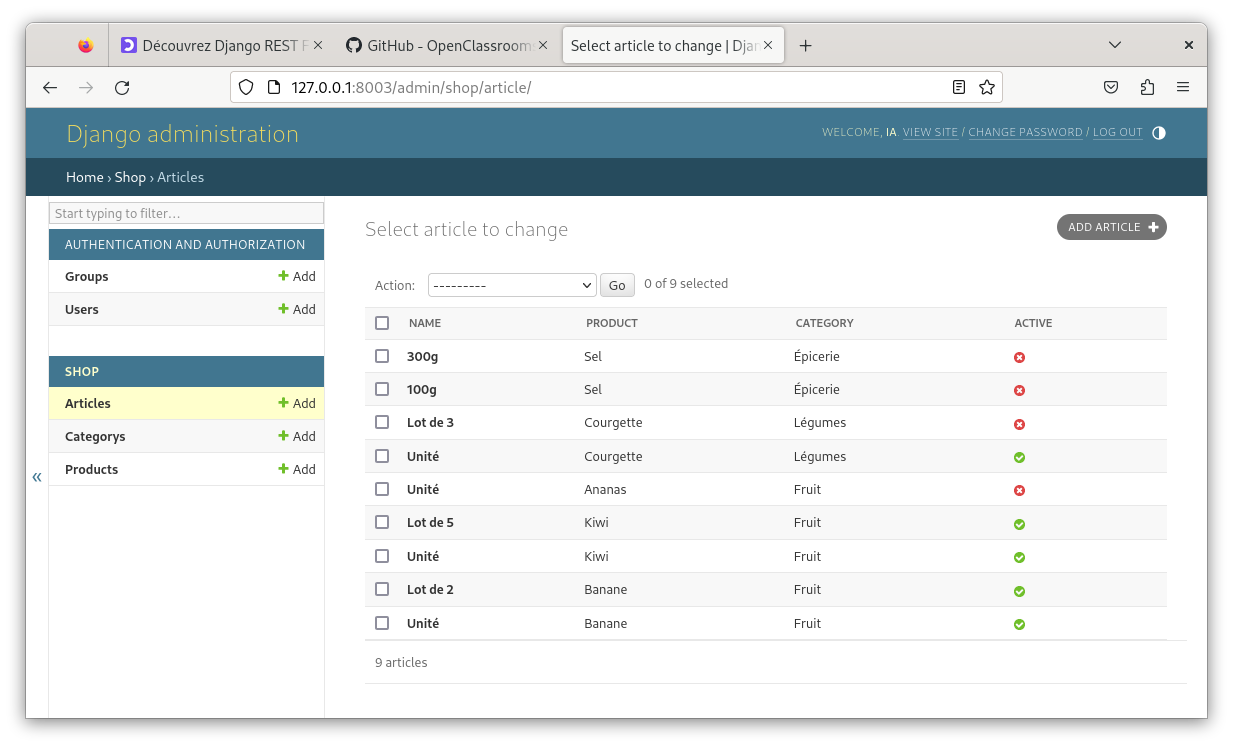
\includegraphics[width=10cm]{images/image04.png}
\end{center}

\subsection{Installation des dépendances}
Pour le moment, {\color{monOrange}create-vue} a déclaré toutes les dépendances et les configurations nécessaires en suivant vos options. Aucune dépendance {\tt JavaScript} n'a encore été installée par {\tt npm}. Pour les installer, il suffit d'ouvrir un terminal et d'aller dans le dossier de votre application, par exemple :
\begin{minted}[
mathescape,
framesep=2mm,
baselinestretch=1.2,
fontsize=\footnotesize,
bgcolor=LightGray,
%linenos
]{bash}
cd dymaproject
\end{minted}

Et ensuite de lancer l'installation des dépendances :
\begin{minted}[
mathescape,
framesep=2mm,
baselinestretch=1.2,
fontsize=\footnotesize,
bgcolor=LightGray,
%linenos
]{bash}
npm install
\end{minted}

\subsection{Utilisation du linter}
Un linter est un outil d'analyse de code qui permet de détecter les erreurs et les problèmes de syntaxe. La configuration du linter, en l'occurrence {\tt ESLint} est dans le fichier {\tt .eslintrc.cjs} :
\begin{minted}[
mathescape,
framesep=2mm,
baselinestretch=1.2,
fontsize=\footnotesize,
bgcolor=LightGray,
%linenos
]{javascript}
/* eslint-env node */
require('@rushstack/eslint-patch/modern-module-resolution')

module.exports = {
  root: true,
  'extends': [
    'plugin:vue/vue3-essential',
    'eslint:recommended',
    '@vue/eslint-config-typescript',
    '@vue/eslint-config-prettier/skip-formatting'
  ],
  parserOptions: {
    ecmaVersion: 'latest'
  }
}
\end{minted}

{\color{monOrange} create-vue} a donc automatiquement créé la bonne configuration du linter pour une utilisation avec {\tt Vue.js}. Pour exécuter le linter avec la configuration faites :

\begin{minted}[
mathescape,
framesep=2mm,
baselinestretch=1.2,
fontsize=\footnotesize,
bgcolor=LightGray,
%linenos
]{bash}
npm run lint
\end{minted}     

Cela exécutera le script {\tt lint} déclaré dans le fichier {\tt package.json}. Pour l'instant il y a bien sûr aucune indication car nous n'avons pas commencé à coder ! Mais exécuter cette commande de temps en temps lors du développement permet d'éviter certaines erreurs et de suivre les recommandations pour les bonnes pratiques en matière de syntaxe (appelées coding style).

\subsection{Lancer le serveur de développement}
Pour lancer le serveur de développement il suffit d'exécuter le script dev :
\begin{minted}[
mathescape,
framesep=2mm,
baselinestretch=1.2,
fontsize=\footnotesize,
bgcolor=LightGray,
%linenos
]{bash}
npm run dev
\end{minted} 

Cela va en fait exécuter {\color{monOrange}vite} qui va lancer son serveur de développement. Vous pourrez ainsi accéder à l'application {\tt Vue.js} dans votre navigateur à l'adresse {\color{monOrange} http://localhost:5173/}.

\begin{center}
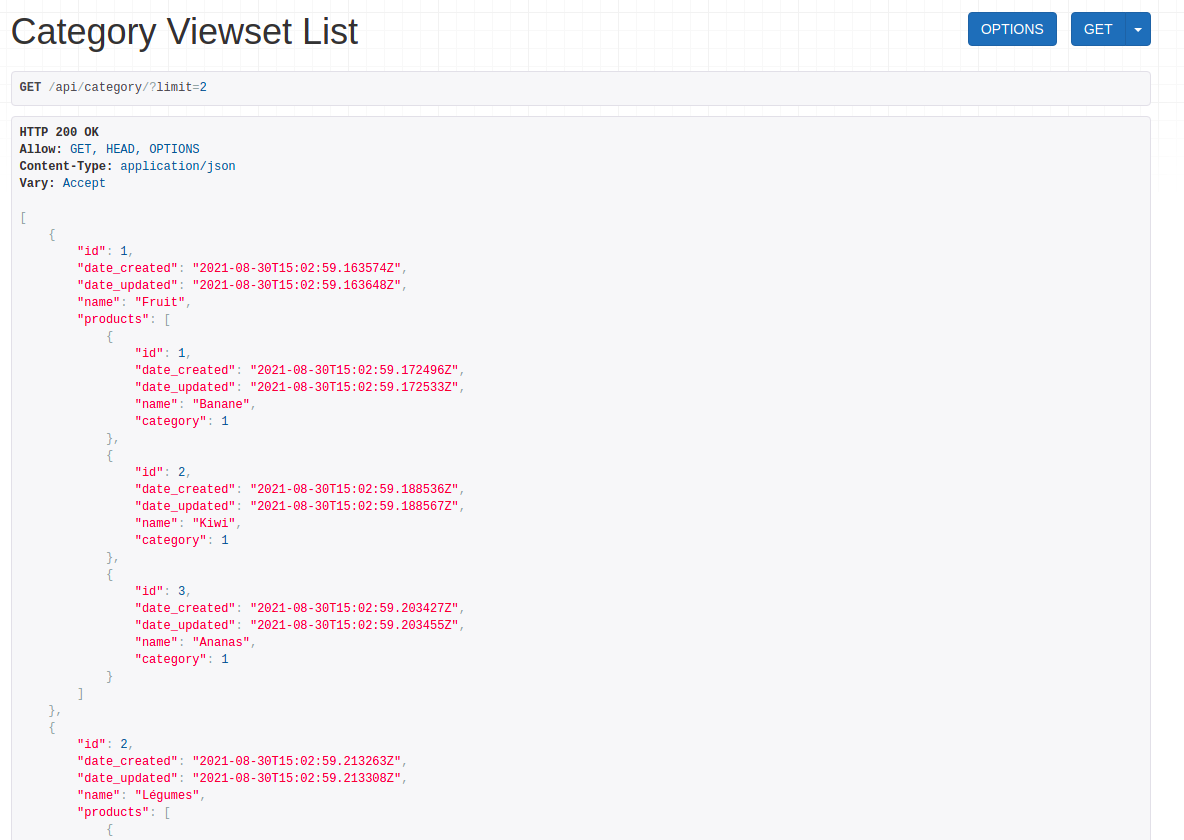
\includegraphics[width=10cm]{images/image13.png}
\end{center}

%%%%%%%%%%%%%%%%%%%%%%%%%%%%%%%%%%%%%%%%%%%%%%%%%%%%%%%%%%%%%%%%%
\section{Architecture initiale}
\subsection{Architecture initiale d'un projet généré par create-vue}
L'architecture initiale du projet généré est la suivante :
\begin{center}
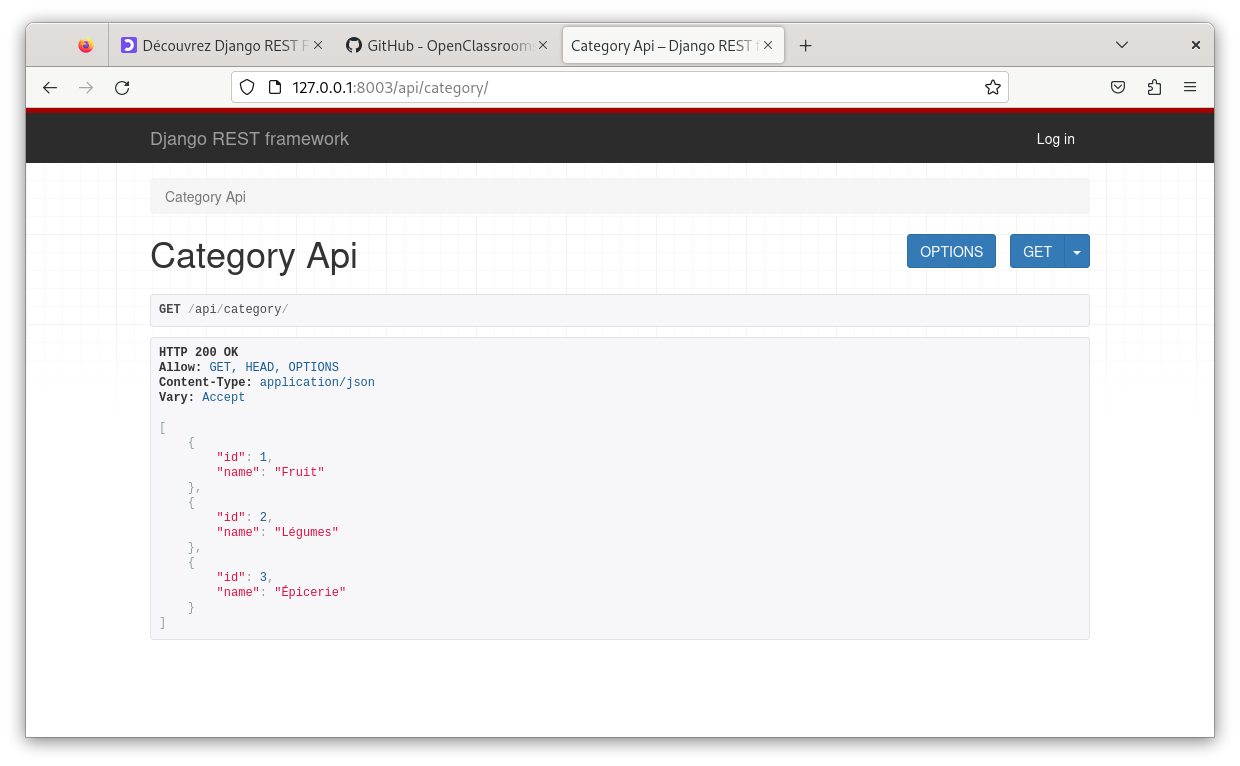
\includegraphics[width=3cm]{images/image05.png}
\end{center}

\subsection{Détail des fichiers et des dossiers}
\begin{itemize}
\item {\tt vite.config.js} : fichier de configuration de Vite.
\item {\tt tsconfig.node.json} : fichier de configuration de Vite pour pouvoir utiliser TypeScript. Vous pouvez retirer vitest, cypress, playwright de la propriété types car nous ne les utiliserons pas pour le moment :


\begin{minted}[
mathescape,
framesep=2mm,
baselinestretch=1.2,
fontsize=\footnotesize,
bgcolor=LightGray,
%linenos
]{javascript}
{
  "extends": "@vue/tsconfig/tsconfig.node.json",
  "include": ["vite.config.*"],
  "compilerOptions": {
    "composite": true,
    "types": ["node"]
  }
}
\end{minted} 
\item {\tt tsconfig.json} : fichier de configuration de TypeScript. Toutes les applications utilisant TypeScript ont ce fichier. Il permet de configurer notamment les options pour transpiler le TypeScript en JavaScript.
\item {\tt README.md} : décrit brièvement les différentes commandes possibles et la configuration recommandée de l'éditeur VS Code.
\item {\tt package.json} et {\tt package-lock.json} : ces fichiers {\tt JSON} permettent de décrire le projet et surtout de détailler les dépendances et leurs versions requises pour l'utiliser. Il décrit également les scripts pouvant être lancés avec {\color{monOrange}npm run}.
\end{itemize}
Les scripts disponibles sont :
\begin{itemize}
\item {\color{blue} dev} : qui permet de lancer le serveur de développement de {\color{monOrange} Vite} en local.
\item  {\color{blue} build} : qui permet de construire la version de l'application optimisée pour la production.
\item  {\color{blue} preview}  : qui permet de visualiser la version de production en local (par exemple avant de la mettre réellement en production sur des serveurs).
\item  {\color{blue} typecheck}  : qui permet de vérifier les types du code {\color{monOrange} TypeScript} sans transpiler le {\color{monOrange} TypeScript} en {\tt JavaScript}.
\item  {\color{blue} lint}  : qui permet d'exécuter {\color{monOrange} ESLint} avec les bonnes options.
\item  {\color{blue} index.html } : template {\tt HTML} qui sera envoyé au navigateur.
\item  {\color{blue} env.d.ts}  : fichier qui permet de charger des types supplémentaires pour utiliser {\color{monOrange} TypeScript} avec {\color{monOrange} Vue.js}.
\item  {\color{blue} .gitignore}  : permet de lister les fichiers qui ne doivent pas être pris en compte par {\color{monOrange} Git}.

\item  {\color{blue} .eslintrc}  : fichier de configuration de {\color{monOrange} ESLint} que nous avons déjà expliqué.
\item  {\color{blue} src } : dossier qui contient les fichiers sources de votre application (d'où le nom {\color{monOrange} src} pour source).
\item  {\color{blue} public}  : dossier qui contient les fichiers qui n'ont pas besoin d'être traité par {\color{monOrange} Vite} ou par aucun outil et qui sont directement envoyés par le serveur au navigateur.
\item  {\color{blue} src/main.ts}  : il s'agit du point d'entrée de notre application. Nous expliquerons plus loin dans le cours la fonction {\tt createApp()} ainsi que {\tt \$mount}. Sachez simplement que nous importons notre composant racine {\color{monOrange} App} et créons l'instance racine de l'application ici.
\item  {\color{blue} src/App.vue}  : il s'agit du composant référencé dans {\color{monOrange} main.ts} qui constitue la racine des vues de notre application. Il s'agit du premier composant rendu, et de lui découle les rendus de tous les autres composants. Nous étudierons la structure des composants dans une prochaine leçon.
\item  {\color{blue} src/components}  : dossier qui contient les composants de notre application {\color{monOrange} Vue}.
\item  {\color{blue} src/components/HelloWorld.vue}  : sous-composant de {\color{monOrange} App.vue}.
\item  {\color{blue} src/assets}  : dossier contenant les ressources de l'application comme les images, le {\tt CSS} etc.
\item  {\color{blue} node\_modules}  : contient toutes les dépendances installées par {\color{monOrange} npm}.
\end{itemize}

%%%%%%%%%%%%%%%%%%%%%%%%%%%%%%%%%%%%%%%%%%%%%%%%%%%%%%%%%%%%%%%%%%%%%%%%%


\section{Comment fonctionne Vue ?}
Nous allons voir les fichiers par ordre logique. Le navigateur reçoit en premier l'{\color{monOrange}index.html}.

\subsection{Le fichier {\color{monOrange}index.html}}
Le fichier index.html est ce que le navigateur va lire en premier :
\begin{minted}[
mathescape,
framesep=2mm,
baselinestretch=1.2,
fontsize=\footnotesize,
bgcolor=LightGray,
%linenos
]{html}
<!DOCTYPE html>
<html lang="en">
  <head>
    <meta charset="UTF-8" />
    <link rel="icon" href="/favicon.ico" />
    <meta name="viewport" content="width=device-width, initial-scale=1.0" />
    <title>Vite App</title>
  </head>
  <body>
    <div id="app"></div>
    <script type="module" src="/src/main.ts"></script>
  </body>
</html>
\end{minted} 

Notez bien qu'il y a une {\tt div} conteneur avec l'{\color{monOrange}id app}. Notez également que le fichier src/main.ts est chargé comme un module {\tt JavaScript}. Le navigateur demande donc ce module au serveur.

\subsection{Le fichier {\color{monOrange}src/main.ts}}
Le fichier {\color{monOrange}main.ts} est le point d'entrée de l'application car c'est le premier fichier {\tt JavaScript} chargé par le navigateur.

Note : le fichier est en {\color{monOrange}.ts} car c'est un fichier {\tt TypeScript} mais il sera transpilé par Vite en {\tt JavaScript} que ce soit pour le développement ou la production. En effet, le navigateur ne comprend que le langage {\tt JavaScript} et pas le {\tt TypeScript}.
\begin{minted}[
mathescape,
framesep=2mm,
baselinestretch=1.2,
fontsize=\footnotesize,
bgcolor=LightGray,
%linenos
]{javascript}
import { createApp } from "vue";
import App from "./App.vue";

createApp(App).mount("#app");
\end{minted} 

{\tt import App from "./App.vue";} permet d'importer le composant {\color{monOrange}App} que nous verrons juste après. {\tt createApp()} permet de créer une instance de votre application {\color{monOrange}Vue.js}. Elle prend en argument, le composant racine, c'est-à-dire le premier composant de votre application qui aura d'autres composants enfants.

{\tt mount()} permet de monter l'application instanciée par {\tt createApp()} dans un conteneur qui est identifié par un sélecteur {\tt CSS}. Ici, cela signifie que le composant racine {\color{monOrange}App} sera monté sur le conteneur dont l'{\color{monOrange}id} est {\color{monOrange}app} :
\begin{minted}[
mathescape,
framesep=2mm,
baselinestretch=1.2,
fontsize=\footnotesize,
bgcolor=LightGray,
%linenos
]{html}
<div id="app"></div>
\end{minted} 

Le composant sera ainsi affiché (on dit plus souvent rendu) dans ce conteneur.

\subsection{Le fichier {\color{monOrange}src/App.vue}}
Le fichier {\tt App.vue} est le composant racine. C'est le premier composant de l'application qui est chargé et instancié par {\tt createApp()}. Ce composant est le sommet de ce qu'on appelle l'arbre des composants : à savoir l'organisation hiérarchique des composants de l'application. Une application a des dizaines voir des centaines de composants qui sont organisés en arbre à partir du composant racine :
\begin{center}
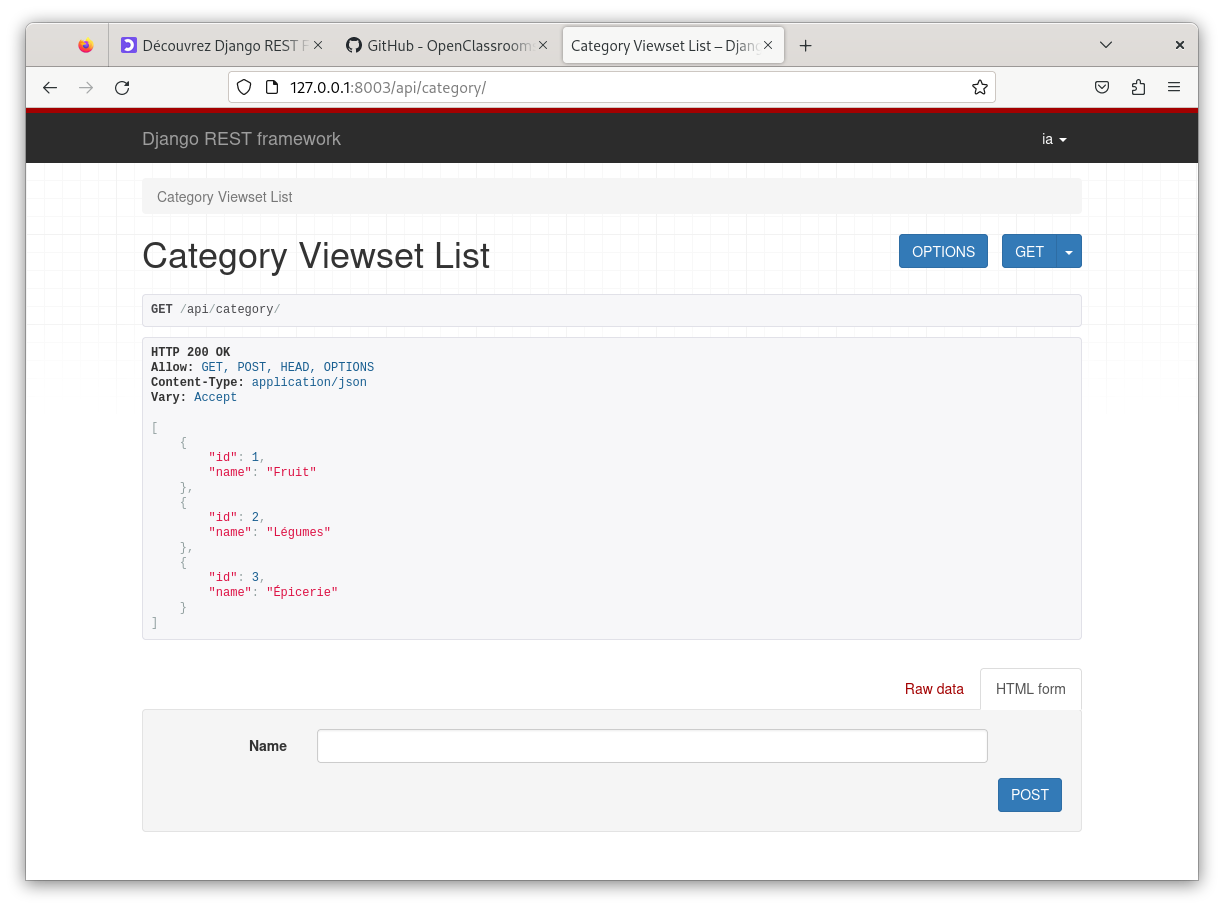
\includegraphics[width=12cm]{images/image06.png}
\end{center}

Remarquez déjà que le composant {\color{monOrange}App.vue} est constitué de trois parties : {\tt template, script} et {\tt style}. Nous étudierons bientôt les composants en détail.

\subsection{Aller plus loin sur le fonctionnement de Vue.js : le {\color{monOrange}DOM virtuel}}
Nous allons d'abord effectuer quelques rappels avant d'approfondir le fonctionnement de Vue.js.
\subsubsection{Le DOM (Document Object Model)}
Le {\tt DOM} permet de passer du {\tt HTML} à un grand objet document qui est un arbre regroupant tous les éléments déclarés en {\tt HTML}. Autrement dit, lorsque le navigateur reçoit le {\tt HTML} de la page, il va le parser (c'est-à-dire l'analyser) et le transformer en {\tt DOM} grâce à des algorithmes. Ainsi, les attributs {\tt HTML} deviennent automatiquement des propriétés des objets du {\tt DOM}. Par exemple :
\begin{minted}[
mathescape,
framesep=2mm,
baselinestretch=1.2,
fontsize=\footnotesize,
bgcolor=LightGray,
%linenos
]{html}
<body id="page">
\end{minted} 

Devient un nœud sur l'objet document qui sera un objet body contenant une propriété id contenant la valeur page.

Il existe plusieurs types de noeuds :
\begin{center}
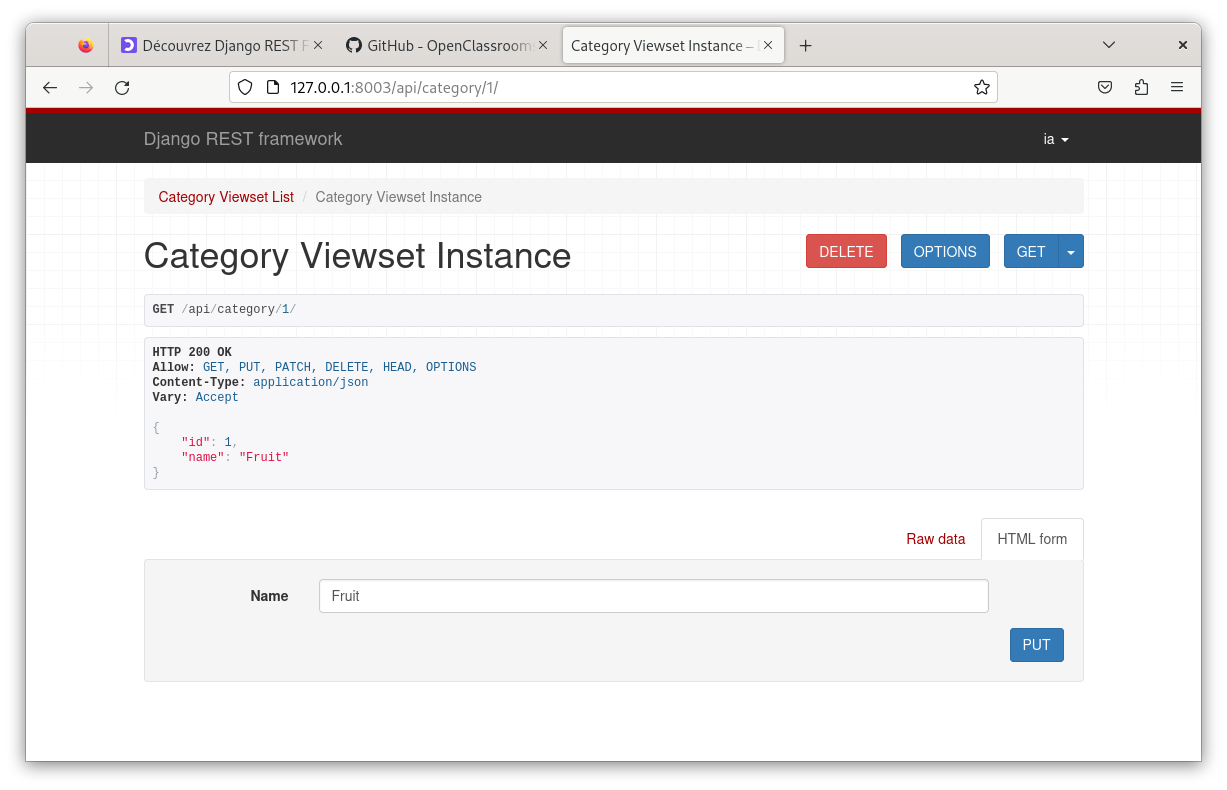
\includegraphics[width=15cm]{images/image07.png}
\end{center}

\subsubsection{Le DOM virtuel}
Dans les applications Web modernes, il peut y avoir des centaines ou des milliers de nœuds sur lesquels sont enregistrés de nombreux gestionnaires d'événements. En conséquence, de très nombreuses mises à jour du {\tt DOM} doivent être réalisées. Or, ces mises à jour sont très coûteuses en performance car plus le {\tt DOM} est grand, plus les recherches et les changements sont coûteux. {\color{monOrange}Vue.js} utilise donc un {\tt DOM} virtuel (appelé {\tt VDOM}) qui est une représentation du {\tt DOM} en {\tt JavaScript}. Le {\tt DOM } virtuel n'est donc qu'un simple, immense, objet {\tt JavaScript} :
\begin{minted}[
mathescape,
framesep=2mm,
baselinestretch=1.2,
fontsize=\footnotesize,
bgcolor=LightGray,
%linenos
]{javascript}
const vnode = {
  type: 'div',
  props: {
    id: 'hello'
  },
  children: [
    /* plein de vnodes */
  ]
}
\end{minted} 

Les noeuds du DOM virtuels sont appelés des noeuds virtuels ou {\color{monOrange}vnode} (pour virtual node). {\color{monOrange}Vue.js} va transformer le {\tt VDOM} en {\tt DOM} pour que le navigateur puisse afficher la page. Ce processus est appelé le montage (mount en anglais).

Lorsque des mises à jour sur la page doivent intervenir, le {\tt DOM} virtuel est modifié avant que les modifications sur le {\tt DOM} ne soient effectuées. Le {\tt DOM} virtuel est une représentation légère du {\tt DOM} en {\tt JavaScript} qui peut être utilisée par des algorithmes très performants de comparaison des différences entre {\tt DOM} virtuel et {\tt DOM}.

Dès lors que le {\tt DOM} doit être modifié, un patch est appliqué par {\color{monOrange}Vue.js} de manière extrêmement optimisée pour ne réaliser que les changements absolument nécessaires. Par exemple, si aucune valeur affichée ne change, alors aucune mise à jour du {\tt DOM} n'est déclenchée ce qui économise beaucoup en performance.

En résumé, {\color{monOrange}Vue.js} va créer au départ un {\tt DOM} virtuel puis le convertir en {\tt DOM HTML} pour l'affichage lors du montage. Lorsque des changements interviennent, par exemple un événement survient, les changements affectant le {\tt DOM} virtuel sont analysés par des algorithmes et seuls les changements ayant un effet sur l'affichage sont propagés au {\tt DOM} lors de la phase de mise à jour (patch ou diffing en anglais). Ainsi, seules les insertions, les modifications et les suppressions d'éléments {\tt HTML} absolument nécessaires sont effectuées, ce qui permet un énorme gain de performance.

%%%%%%%%%%%%%%%%%%%%%%%%%%%%%%%%%%%%%%%%%%%%%%%%%%%%%%%%%%%

\section{Les API composition et options}
{\color{monOrange}Vue.js} propose deux API pour écrire des composants {\color{monOrange}Vue} : l'API options et l'API composition.
\begin{itemize}
\item L'API options est l'API originelle qui existe depuis la première version du {\color{monOrange}framework}.
\item L'API composition est l'API avec laquelle {\color{monOrange}Vue} a été réécrite pour la version 3. C'est la nouvelle API qui est aujourd'hui recommandée et celle que nous verrons dans la formation.
\end{itemize}
\subsection{L'API options}
Dans l'ancienne API options, la logique du composant est définie dans un objet comportant des options comme {\tt data}, {\tt methods} ou {\tt mounted} par exemple. Les propriétés sont définies sur l'objet {\tt this} disponible dans les options.

Nous ne détaillerons pas plus car ce n'est pas l'API que nous utiliserons. Nous la présentons uniquement pour que vous puissiez la reconnaître lorsque vous la rencontrez. Voici à quoi ressemble un composant écrit avec l'API options :
\begin{minted}[
mathescape,
framesep=2mm,
baselinestretch=1.2,
fontsize=\footnotesize,
bgcolor=LightGray,
%linenos
]{html}
<script>
export default {
  data() {
    return {
      count: 0
    }
  },
  methods: {
    increment() {
      this.count++
    }
  },
  mounted() {
    console.log(`La valeur initiale est ${this.count}.`)
  }
}
</script>

<template>
  <button @click="increment">Valeur du compteur : {{ count }}</button>
</template>
\end{minted} 

\subsection{L'API composition}
Avec l'API composition nous définissons la logique d'un composant en important des fonctions. Voilà le même exemple avec la nouvelle API :
\begin{minted}[
mathescape,
framesep=2mm,
baselinestretch=1.2,
fontsize=\footnotesize,
bgcolor=LightGray,
%linenos
]{html}
<script setup>
import { ref, onMounted } from 'vue'

const count = ref(0)
function increment() {
  count.value++
}

onMounted(() => {
  console.log(`La valeur initiale est ${count.value}.`)
})
</script>

<template>
  <button @click="increment">Valeur du compteur : {{ count }}</button>
</template>
\end{minted} 

\subsection{Les {\color{monOrange}Single-File Components} (SFC)}
Les SFC sont des composants écrits dans des fichiers qui terminent par l'extension {\color{monOrange}.vue}. Un SFC comporte la logique du composant (partie script en {\tt JavaScript/TypeScript}), le template (en {\tt HTML}) et le style (en {\tt CSS} ou {\tt Sass}).

Il est fortement recommandé d'utiliser les SFC pour écrire des composants {\color{monOrange}Vue.js}. C'est d'ailleurs ce que nous utiliserons tout le long de la formation.

%%%%%%%%%%%%%%%%%%%%%%%%%%%%%%%%%%%%%%%%%%%%%%%%%%%%%%%

\section{Création d'un composant}
\subsection{Passer en mode {\color{monOrange}Take Over}}
L'extension {\color{monOrange}Volar} est plus performante pour gérer l'utilisation de {\tt TypeScript} avec {\color{monOrange}Vue.js}. Aussi, il faut configurer l'éditeur {\tt VS Code} pour lui dire que nous utilisons {\color{monOrange}Volar}.

Pour ce faire, aller sur l'onglet {\tt Extensions de VS Code}. Recherchez {\tt @builtin typescript}. Cliquez sur {\tt TypeScript and JavaScript Language Features}. Cliquez sur {\tt Désactiver (espace de travail)}. Cela désactivera uniquement pour ce projet. Cliquez ensuite sur Rechargement requis.

\subsection{Utilisation du mode {\color{monOrange}strict} de {\color{monOrange}TypeScript}}
Pour activer l'option {\color{monOrange}strict} du compilateur {\tt TypeScript} modifiez le fichier {\tt tsconfig.json} :
\begin{minted}[
mathescape,
framesep=2mm,
baselinestretch=1.2,
fontsize=\footnotesize,
bgcolor=LightGray,
%linenos
]{javascript}
{
  "extends": "@vue/tsconfig/tsconfig.web.json",
  "include": ["env.d.ts", "src/**/*", "src/**/*.vue"],
  "compilerOptions": {
    "strict": true,
    "baseUrl": ".",
    "paths": {
      "@/*": ["./src/*"]
    }
  },
  "references": [
    {
      "path": "./tsconfig.node.json"
    }
  ]
}
\end{minted} 

Cette option permet d'activer de nombreuses configurations plus strictes pour le contrôle des types par le compilateur. Cela permet d'améliorer sa capacité à détecter des erreurs.

\subsection{Création du premier composant}
Commençons par supprimer les composants mis en place automatiquement par {\color{monOrange}create-vue} pour la page de présentation lors du lancement de l'application. 
\begin{enumerate}
\item Supprimez tous les fichiers et les dossiers dans {\tt src/components/}.
\item Supprimez le contenu, mais pas le fichier de {\tt src/App.vue}.
\end{enumerate}

Comme nous l'avons vu, un composant {\color{blue} monofichier} (SFC, pour Single-file component) est un fichier {\color{blue} .vue} dont le nom est par convention en {\tt PascalCase}. Un composant monofichier a donc un template qui comporte le {\tt HTML}, une partie script qui comporte le JavaScript et une partie style qui comporte le {\tt CSS}. Voici l'exemple minimal de la vidéo :
\begin{minted}[
mathescape,
framesep=2mm,
baselinestretch=1.2,
fontsize=\footnotesize,
bgcolor=LightGray,
%linenos
]{html}
<template>
    <h1>Bonjour {{name}}</h1>
</template>

<script setup lang="ts">
    const name = 'Jean';
</script>

<style></style>
\end{minted} 

%\subsection{Exemple exécutable}
%Vous pouvez aussi directement utiliser ce code exécutable. N'hésitez pas à l'ouvrir dans un nouvel onglet :

%%%%%%%%%%%%%%%%%%%%%%%%%%%%%%%%%%%%%%%%%%%%%%%%%%%%%%

\section{Vue.js sans Vite}
\subsection{Utiliser {\color{monOrange}Vue.js} sans {\color{monOrange}Vite}}
Créez un dossier projet-vue.

Dans ce dossier, créez un fichier index.html :
\begin{minted}[
mathescape,
framesep=2mm,
baselinestretch=1.2,
fontsize=\footnotesize,
bgcolor=LightGray,
%linenos
]{html}
<!DOCTYPE html>
<html lang="en">
  <head>
    <meta charset="UTF-8" />
    <meta http-equiv="X-UA-Compatible" content="IE=edge" />
    <meta name="viewport" content="width=device-width, initial-scale=1.0" />
    <title>Document</title>
    <script src="https://unpkg.com/vue@3"></script>
  </head>
  <body>
    <div id="app">
      <h1>Bonjour {{ name }}</h1>
    </div>

    <script>
      Vue.createApp({
        setup() {
          const name = 'test';
          return {
            name,
          };
        },
      }).mount('#app');
    </script>
  </body>
</html>
\end{minted} 

Ici, nous n'utilisons que la librairie {\color{monOrange}Vue.js} sans {\color{monOrange}Vite} et sans aucune autre librairie. 
\begin{itemize}
\item Il n'y a aucune étape de {\tt build}, nous ne pouvons pas utiliser Sass, TypeScript etc.

\item Il n'y a pas de minification du code et pleins d'avantages apportés par {\color{monOrange}Vite}.
\end{itemize}
Cet exemple permet simplement de montrer comment utiliser {\color{monOrange}Vue.js} seul mais dans toute la formation nous n'utiliserons pas du tout cette méthode car il est impossible d'écrire une application complexe comme cela. Cette manière de faire peut être utile pour par exemple gérer une barre de recherche sur une application avec {\color{monOrange}Symfony} côté serveur.

	\chapter{Intéragir avec le DOM}
	\section{Introduction aux directives}
\subsection{Les directives}
Les directives sont des attributs spéciaux avec le préfixe {\color{monOrange}v-}. L'objectif d'une directive est d'appliquer de manière réactive des effets au {\tt DOM} lorsque la valeur de son expression change. Les directives natives sont les suivantes :
\begin{itemize}
\item v-text (qui équivaut à {{ }})
\item v-bind
\item v-html
\item v-once
\item v-show
\item v-if
\item v-else
\item v-else-if
\item v-for
\item v-on
\item v-model
\item v-pre
\item v-cloak
\item v-slot
\item v-memo
\end{itemize}

Il est également possible, comme nous l'étudierons, de créer ses propres directives {\color{monOrange}Vue}. Commençons par la directive la plus simple v-text.

\subsection{La directive {\color{monOrange}v-text} et l'interpolation de texte}
La directive {\color{monOrange}v-text} permet de mettre à jour le contenu de la propriété textContent de l'élément {\tt HTML}. La directive prend en argument la propriété déclarée sur le composant dont la valeur doit être utilisée. On appelle cela l'interpolation de texte. Par exemple, s'il existe une propriété message sur le composant dans la partie script, alors nous pouvons utiliser la directive de cette manière côté template :
\begin{minted}[
mathescape,
framesep=2mm,
baselinestretch=1.2,
fontsize=\footnotesize,
bgcolor=LightGray,
%linenos
]{html}
<span v-text="message"></span>
\end{minted}

La propriété {\color{blue}textContent} de l'élément {\tt span} sera alors remplacé par la valeur de la propriété {\tt message}. Comme lier une propriété est extrêmement courant, il existe une forme raccourcie appelée la notation moustache (de part sa forme), utilisant deux paires d'accolades :
\begin{minted}[
mathescape,
framesep=2mm,
baselinestretch=1.2,
fontsize=\footnotesize,
bgcolor=LightGray,
%linenos
]{html}
<span>{{message}}</span>
\end{minted}

Est du sucre syntaxique pour :
\begin{minted}[
mathescape,
framesep=2mm,
baselinestretch=1.2,
fontsize=\footnotesize,
bgcolor=LightGray,
%linenos
]{html}
<span v-text="message"></span>
\end{minted}

Note : en programmation, on appelle sucre syntaxique une syntaxe plus concise ou plus élégante qui est remplacée automatiquement par le code complet et donne le même résultat qu'une expression plus longue.

\subsection{Utilisation d'expression JavaScript}
Avec {\color{monOrange}Vue.js} il est possible d'utiliser toute expression {\tt JavaScript} valide comme argument d'une directive. Voici un exemple avec un ternaire :
\begin{minted}[
mathescape,
framesep=2mm,
baselinestretch=1.2,
fontsize=\footnotesize,
bgcolor=LightGray,
%linenos
]{javascript}
{{ condition ? 'Oui' : 'Non' }}
\end{minted}
Autre exemple :
\begin{minted}[
mathescape,
framesep=2mm,
baselinestretch=1.2,
fontsize=\footnotesize,
bgcolor=LightGray,
%linenos
]{javascript}
{{ message.reverse().toUpperCase() }}
\end{minted}

Encore un autre :
\begin{minted}[
mathescape,
framesep=2mm,
baselinestretch=1.2,
fontsize=\footnotesize,
bgcolor=LightGray,
%linenos
]{html}
<h1>Bonjour {{ `${prenom.toLowerCase()} ${nom.toUpperCase()}`}}</h1>
\end{minted}

Nous verrons énormément d'exemples au cours de la formation.

%Exemple exécutable
%Vous pouvez aussi directement utiliser ce code exécutable. N'hésitez pas à l'ouvrir dans un nouvel onglet :

\section{Directive {\color{monOrange}v-html}}
La directive {\color{monOrange}v-html} permet de mettre à jour l'attribut {\color{monOrange}innerHTML} d'un élément. Le contenu sera inséré comme du HTML simple.

Attention ! Le rendu dynamique de HTML sur votre site Web peut être très dangereux car il peut facilement conduire à des attaques {\tt XSS}. Utilisez uniquement {\color{monOrange}v-html} sur un contenu sûr et jamais sur du contenu fourni par l'utilisateur. Voici un exemple :
\begin{minted}[
mathescape,
framesep=2mm,
baselinestretch=1.2,
%fontsize=\footnotesize,
bgcolor=LightGray,
%linenos
]{html}
<p>Contenu HTML: <span v-html="varHtml"></span></p>
\end{minted}

%Exemple exécutable
%Vous pouvez aussi directement utiliser ce code exécutable. N'hésitez pas à l'ouvrir dans un nouvel onglet :

\section{Liaison de propriété avec v-bind}
La directive v-bind permet d'associer dynamiquement un attribut à une propriété.
\subsection{Syntaxe de base}
Elle prend en argument l'attribut auquel la propriété est liée. Ainsi par exemple :
\begin{minted}[
mathescape,
framesep=2mm,
baselinestretch=1.2,
%fontsize=\footnotesize,
bgcolor=LightGray,
%linenos
]{html}
<a v-bind:href="url"></a>
\end{minted}

L'attribut href de l'ancre est liée ici à la valeur de la variable url grâce à l'utilisation de la directive v-bind.

\subsection{Syntaxe raccourcie}
Comme cette directive est extrêmement utilisée, il existe une forme raccourcie :
\begin{minted}[
mathescape,
framesep=2mm,
baselinestretch=1.2,
%fontsize=\footnotesize,
bgcolor=LightGray,
%linenos
]{html}
<a :href="url"></a>
\end{minted}
C'est cette forme que nous utiliserons dans la formation et qui est recommandée.
\subsection{Utilisation sur des attributs booléens}
Les attributs booléens sont les attributs pour lesquels la simple présence de l'attribut représente la valeur true et leur absence la valeur false. Il y en a 26 différents.

Des exemples sont : disabled, checked, multiple, readonly, selected, hidden etc. Lorsque la directive v-bind est utilisée sur un attribut booléen, le comportement est le suivant : si la variable liée vaut true alors l'attribut sera ajouté par Vue.js automatiquement, si la variable vaut false alors l'attribut sera retiré. Par exemple :

\begin{minted}[
mathescape,
framesep=2mm,
baselinestretch=1.2,
%fontsize=\footnotesize,
bgcolor=LightGray,
%linenos
]{html}
<button :disabled="isButtonDisabled">Button</button>
\end{minted}

Si isButtonDisabled vaut true alors l'attribut disabled sera ajouté par Vue.js sur le DOM, s'il vaut false il sera enlevé.

\subsection{Utilisation sur plusieurs attributs}
La directive v-bind peut être utilisée pour lier un objet contenant des paires nom-valeur d'attribut. Exemple :
\begin{minted}[
mathescape,
framesep=2mm,
baselinestretch=1.2,
%fontsize=\footnotesize,
bgcolor=LightGray,
%linenos
]{html}
<div v-bind="{ id: propriété, 'autre-attribut': autrePropriété }"></div>
\end{minted}

Ainsi, si nous avons côté script :
\begin{minted}[
mathescape,
framesep=2mm,
baselinestretch=1.2,
%fontsize=\footnotesize,
bgcolor=LightGray,
%linenos
]{javascript}
const objet = {
  id: 'container',
  class: 'container'
}
\end{minted}

Nous pouvons lier cet objet avec la directive v-bind :
\begin{minted}[
mathescape,
framesep=2mm,
baselinestretch=1.2,
%fontsize=\footnotesize,
bgcolor=LightGray,
%linenos
]{html}
<div v-bind="objet"></div>
\end{minted}

Attention ! Dans ce cas la notation raccourcie n'est pas possible.
\subsection{Utilisation avec class et style}
Lorsqu'elle est utilisée avec les attributs class ou style, la directive v-bind peut prendre un tableau ou un objet en argument de cette façon :
\begin{minted}[
mathescape,
framesep=2mm,
baselinestretch=1.2,
%fontsize=\footnotesize,
bgcolor=LightGray,
%linenos
]{html}
<div :style="{ fontSize: size + 'px' }"></div>
\end{minted}
Ou :
\begin{minted}[
mathescape,
framesep=2mm,
baselinestretch=1.2,
%fontsize=\footnotesize,
bgcolor=LightGray,
%linenos
]{html}
<div :class="[classA, classB]"></div>
\end{minted}

Nous verrons des exemples dans la formation.

\subsection{Utilisation avec un attribut dynamique}
Vous pouvez utiliser une liaison dynamique également sur l'attribut avec cette syntaxe :
\begin{minted}[
mathescape,
framesep=2mm,
baselinestretch=1.2,
%fontsize=\footnotesize,
bgcolor=LightGray,
%linenos
]{html}
<button :[clé]="valeur"></button>
\end{minted}
Ici l'attribut peut être modifié dynamiquement en modifiant la valeur de la variable clé.

%Exemple exécutable
%Vous pouvez aussi directement utiliser ce code exécutable. N'hésitez pas à l'ouvrir dans un nouvel onglet :

\section{Utilisation de fonction dans les liaisons}
Comme nous l'avons vu, il est possible d'utiliser des expressions {\tt JavaScript} dans les templates. Nous pouvons donc invoquer des fonctions. Il est donc courant de voir :
\begin{minted}[
mathescape,
framesep=2mm,
baselinestretch=1.2,
%fontsize=\footnotesize,
bgcolor=LightGray,
%linenos
]{html}
<span :title="toTitleCase(titre)">
  {{ formatDate(date) }}
</span>
\end{minted}

Ici, nous utilisons deux invocations de fonction. L'une avec {\color{monOrange}v-bind} et l'autre avec {\color{monOrange}v-text}. Nous verrons de nombreux exemples au cours de la formation car c'est très courant.

%Exemple exécutable
%Vous pouvez aussi directement utiliser ce code exécutable. N'hésitez pas à l'ouvrir dans un nouvel onglet :

\section{Notions de base TypeScript}
\subsection{Les types statiques}
{\color{monOrange}TypeScript} permet de tout taper statiquement : vos variables, vos fonctions (arguments, valeur de retour) et vos classes. Le langage ne vous force pas à taper, ce qui vous laisse totalement libre de le faire ou non et ainsi d'adopter progressivement le typage statique en fonction de votre apprentissage.

\subsection{L'inférence de types}
{\color{monOrange}TypeScript}  va détecter automatiquement le type de votre variable en regardant la valeur qui lui est assignée. Nous reviendrons en détails sur cette fonctionnalité très pratique, mais elle permet sans aucune ligne supplémentaire d'avoir ce résultat :
\begin{minted}[
mathescape,
framesep=2mm,
baselinestretch=1.2,
%fontsize=\footnotesize,
bgcolor=LightGray,
%linenos
]{javascript}
const obj = { width: 1, height: 2 };
const aire = obj.width * obj.heigth;
// Property 'heigth' does not exist on type '{ width: number; height: number; }'. Did you mean // 'height'?
\end{minted}

Ici {\color{monOrange}TypeScript}  a détecté qu'aucune propriété {\tt heigth} n'existait sur objet vous invite à vérifier que vous n'avez pas fait une erreur. Magique, non ?

\subsection{Les types}
Comme son nom l'indique et comme nous l'avons vu {\color{monOrange}TypeScript}  est avant tout un langage pour taper. Il est possible de taper absolument tout comme nous le verrons : que ce soit les variables mais aussi les retours de fonction ou des situations encore plus complexes.

Typer au début peut sembler fastidieux : il faut ajouter un peu de code à chaque fois. Mais les bénéfices se remarquent très vite et dans cet ordre souvent :
\begin{enumerate}
\item  Vous aurez moins de bugs lors de l'exécution car beaucoup auront été signalés lors de la compilation : typo dans les noms, erreurs dans les conditions, dans les arguments passés, dans les retours de fonction etc.

\item   {\color{blue} VS} Code vous fournira avec un survol de la souris plein d'informations sur vos fonctions : quels arguments sont attendus etc, et vous gagnerez un temps fou grâce à l'autocomplétion (car  {\color{monOrange}TypeScript}  aura toutes les propriétés sur vos objets etc).

\item   Lorsque vous serez sur un projet à plusieurs, vous pourrez lire et comprendre beaucoup plus vite le code des autres développeurs car vous verrez facilement ce que prend et ce que retourne chaque fonction, quels sont les types acceptés par chaque variable etc.

\end{enumerate}
Une fois les premiers jours, où cela semblera être une surcouche embêtante, passée, vous ne pourrez plus faire sans !

\subsection{Les types primitifs}
Nous allons commencer par les types les plus basiques : les primitifs !

Pour préciser un type en  {\color{monOrange}TypeScript}  nous utilisons la plupart du temps (nous verrons en détails les autres cas) cette syntaxe :
\begin{minted}[
mathescape,
framesep=2mm,
baselinestretch=1.2,
%fontsize=\footnotesize,
bgcolor=LightGray,
%linenos
]{javascript}
variable: type;
\end{minted}

Il est possible de simplement taper une variable sans rien assigner ou de taper et assigner directement :
\begin{minted}[
mathescape,
framesep=2mm,
baselinestretch=1.2,
%fontsize=\footnotesize,
bgcolor=LightGray,
%linenos
]{javascript}
variable: type;
variable: type = x;
\end{minted}

\subsubsection{Les chaînes de caractères :string}
Les chaînes de caractères en {\color{monOrange}TypeScript}  comprennent exactement comme en {\tt JavaScript} les guillemets simples ou doubles et les accents graves ( {\tt backticks}) :
\begin{minted}[
mathescape,
framesep=2mm,
baselinestretch=1.2,
%fontsize=\footnotesize,
bgcolor=LightGray,
%linenos
]{javascript}
let prenom: string = "Jean";
prenom = 'Paul';
prenom = `Patrick`;
\end{minted}

\subsubsection{Les nombres :number}
Tous les nombres valides en {\tt JavaScript} le sont en {\color{monOrange}TypeScript} :
\begin{minted}[
mathescape,
framesep=2mm,
baselinestretch=1.2,
%fontsize=\footnotesize,
bgcolor=LightGray,
%linenos
]{javascript}
let decimal: number = 42;
let flottant: number = 42.22;
let hexadecimal: number = 0x2A;
let binaire: number = 0b101010;
let octal: number = 0o52;
\end{minted}

\subsubsection{Les booléens :boolean}
Le type {\tt boolean} n'accepte que {\tt true} ou {\tt false}:
\begin{minted}[
mathescape,
framesep=2mm,
baselinestretch=1.2,
%fontsize=\footnotesize,
bgcolor=LightGray,
%linenos
]{javascript}
let actif: boolean;
actif = true;
actif = false;
\end{minted}

\subsection{Le type any}
Il est possible de ne pas connaître le type de variables. Ces valeurs peuvent provenir d'un contenu dynamique, par exemple de l'utilisateur ou d'une bibliothèque tierce.

Il est également possible que vous souhaitiez taper plus tard votre fonction ou variable ou que vous soyez en train de convertir un fichier {\tt JavaScript} en {\color{monOrange}TypeScript} et que vous mettiez les types peu à peu.

Dans ces cas, nous souhaitons désactiver la vérification de type. Pour ce faire, nous les étiquetons avec le type {\color{blue}any}.
\begin{minted}[
mathescape,
framesep=2mm,
baselinestretch=1.2,
%fontsize=\footnotesize,
bgcolor=LightGray,
%linenos
]{javascript}
let pasSur: any = 4;
pasSur = 'en fait une string';
\end{minted}

Lorsque vous commencez en {\color{monOrange}TypeScript} vous aurez tendance à beaucoup trop utiliser {\color{blue} any}. A chaque fois que vous ne saurez pas trop le type vous mettrez {\color{blue} any}. Au début ce n'est pas très grave mais il faut vous forcer à faire l'effort de tout bien typer pour garder les bénéfices de l'usage de  {\color{monOrange}TypeScript}. Nous vous recommandons de ne quasiment jamais utiliser {\color{blue} any} sauf dans les cas vus ci-dessus.

\subsection{Le type {\color{monOrange}object}}
Le type {\color{monOrange}objet} permet simplement de représenter le type {\color{blue}non primitif} : tout ce qui n'est pas {\tt number, string, boolean, bigint, symbol, null} ou {\tt undefined}. Cela peut donc être un tableau, un objet littéral, etc.
\begin{minted}[
mathescape,
framesep=2mm,
baselinestretch=1.2,
%fontsize=\footnotesize,
bgcolor=LightGray,
%linenos
]{javascript}
let monObj: object;
monObj = {};
\end{minted}

Notez que {\color{monOrange}object} et {\color{monOrange}{}} sont deux manières de typer un objet, nous pouvons écrire :
\begin{minted}[
mathescape,
framesep=2mm,
baselinestretch=1.2,
%fontsize=\footnotesize,
bgcolor=LightGray,
%linenos
]{javascript}
let monObj: {};
monObj = {};
\end{minted}

\subsection{Le type {\color{monOrange}array}}
Il y a deux syntaxes en {\tt TypeScript} pour taper les {\color{monOrange}tableaux} . En {\tt TypeScript} un tableau est un tableau {\tt JavaScript} contenant un nombre indéfini d'éléments . Première possibilité :
\begin{minted}[
mathescape,
framesep=2mm,
baselinestretch=1.2,
%fontsize=\footnotesize,
bgcolor=LightGray,
%linenos
]{javascript}
type[];
\end{minted}

Où type est le type des éléments contenus dans un tableau. Il est possible d'accepter par exemple que les nombres :
\begin{minted}[
mathescape,
framesep=2mm,
baselinestretch=1.2,
%fontsize=\footnotesize,
bgcolor=LightGray,
%linenos
]{javascript}
let liste: number[] = [1, 2, 3];
\end{minted}
Tous les types :
\begin{minted}[
mathescape,
framesep=2mm,
baselinestretch=1.2,
%fontsize=\footnotesize,
bgcolor=LightGray,
%linenos
]{javascript}
let liste: any[] = [1, true, {}];
\end{minted}

\subsection{Qu'est-ce qu'une {\color{monOrange}interface} ?}
Une {\color{monOrange}interface} est un contrat qui définit la forme qui doit prendre un objet {\tt JavaScript} (objets littéraires, classes et fonctions) . Il est important de noter qu'une {\color{monOrange}interface} n'est pas compilée : aucun code {\tt JavaScript} ne sera créé à partir de l'interface. Elle sert uniquement pour l' IDE, c'est-à-dire pour {\color{blue}VS Code}, (auto-complétions et erreurs de types) et lors de la compilation.

\subsubsection{Notre première interface}
Prenons un premier exemple avec un objet :
\begin{minted}[
mathescape,
framesep=2mm,
baselinestretch=1.2,
%fontsize=\footnotesize,
bgcolor=LightGray,
%linenos
]{javascript}
interface User {
    prenom: string;
}
\end{minted}

Ici, notre objet {\color{monOrange}User} doit obligatoirement avoir une propriété {\color{blue}prenom} contenant une chaîne de caractères. Ensuite nous pouvons utiliser l' interface pour taper par exemple un paramètre d'une fonction :
\begin{minted}[
mathescape,
framesep=2mm,
baselinestretch=1.2,
%fontsize=\footnotesize,
bgcolor=LightGray,
%linenos
]{javascript}
function printUser(user: User) {
    console.log(user.prenom);
}
\end{minted}

Ici, la fonction {\color{blue}printUser} doit recevoir en argument un objet respectant l' interface {\color{monOrange}User} . Par exemple :
\begin{minted}[
mathescape,
framesep=2mm,
baselinestretch=1.2,
%fontsize=\footnotesize,
bgcolor=LightGray,
%linenos
]{javascript}
let paul = {prenom: 'Paul'};
printUser(paul);
\end{minted}

Attention ! Lorsque vous tapez le paramètre de cette manière {\tt user: User} , cela revient à dire que le paramètre doit au moins avoir le ou les propriétés de l'interface {\color{blue}User} et donc avoir une propriété {\tt prenom}.

En revanche, lorsque vous tapez un objet avec une interface, il faut que l'objet respecte exactement l'interface . C'est-à-dire qu'il doit avoir exactement les propriétés définies, ni plus ni moins. Voici un exemple pour bien comprendre :
\begin{minted}[
mathescape,
framesep=2mm,
baselinestretch=1.2,
%fontsize=\footnotesize,
bgcolor=LightGray,
%linenos
]{javascript}
interface User {
    prenom: string;
}

function printUser(user: User) {
    console.log(user.prenom);
}

const paul = {prenom: 'Paul', nom: 'Dupont'};

printUser(paul); // Cela fonctionne car paul a au moins une propriété nom

const jean: User = {prenom: 'Jean', nom: 'Duprey'}; // Erreur
\end{minted}

Dans le cas de l'objet {\color{blue} Jean}, {\tt TypeScript} nous signalons l'erreur suivante : {\bf Type '{ prenom: string; nom: string; }' is not assignable to type 'User'. Object literal may only specify known properties, and 'nom' does not exist in type 'User'}.

Autrement dit, il se plaint car {\color{blue} Jean} a une propriété {\tt nom} qui ne respecte pas le contrat imposé par l' interface {\color{monOrange} User}.

\subsubsection{Les propriétés optionnelles avec?}
Il est possible de définir des propriétés optionnelles comme nous l'avons vu pour les arguments de fonction en utilisant {\color{monOrange} ?}. Ces propriétés sont également utilisables dans les interfaces.
\begin{minted}[
mathescape,
framesep=2mm,
baselinestretch=1.2,
%fontsize=\footnotesize,
bgcolor=LightGray,
%linenos
]{javascript}
interface User {
  prenom: string;
  nom?: string;
}
\end{minted}

Ici, nous établissons comme contrat que les objets qui respecteront l' {\color{monOrange}interface User} auront obligatoirement une propriété {\tt prenom} contenant une chaîne de caractères, et une propriété optionnelle {\tt nom}, qui si elle existe, devra également contenir une chaîne de caractères. En outre, les propriétés optionnelles permettent l'autocomplétion et l'autocorrection.

\subsection{Les unions de type}
Les unions de type permettent de combiner deux ou plusieurs types et s'utilisent avec {\color{monOrange}|} . Les unions s'utilisent dans toutes les situations.

\subsubsection{Unions de type et variables}
Prenons un premier exemple :
\begin{minted}[
mathescape,
framesep=2mm,
baselinestretch=1.2,
%fontsize=\footnotesize,
bgcolor=LightGray,
%linenos
]{javascript}
let uneVar: string | number;}
\end{minted}

Ici, nous effectuons une union entre les types de chaîne de caractères et de nombres. La variable pourra ainsi recevoir l'un des deux types.

\subsubsection{Unions de type et fonctions}
Vous pouvez également taper les paramètres des fonctions en utilisant des unions :
\begin{minted}[
mathescape,
framesep=2mm,
baselinestretch=1.2,
%fontsize=\footnotesize,
bgcolor=LightGray,
%linenos
]{javascript}
function ajouter(a: string | number, b: string | number) {
  return Number(a) + Number(b);
}
\end{minted}

Ici par exemple, notre fonction peut ajouter des nombres et des chaînes de caractères. Nous voulons donc utiliser des unions pour les paramètres de la fonction. Vous pouvez également taper les retours de fonctions en utilisant des unions :
\begin{minted}[
mathescape,
framesep=2mm,
baselinestretch=1.2,
%fontsize=\footnotesize,
bgcolor=LightGray,
%linenos
]{javascript}
function ajouter(isAdmin: boolean): string | void {
  if (isAdmin) {
    return 'secret';
  } else {
    return;
  }
}
\end{minted}


%Exemple exécutable
%Vous pouvez également utiliser directement ce code exécutable. N'hésitez pas à l'ouvrir dans un nouvel onglet :

\section{Les événements natifs}
\subsection{La gestion des événements}
L'objectif de la gestion des événements est de pouvoir réagir à un évènement. Les événements HTML sont des événements qui se produisent suite aux interactions de l'utilisateur avec son clavier, sa souris ou alors à la modification d'éléments du DOM:
\begin{itemize}
\item {\em modification de l'objet {\color{monOrange}window}} : par exemple la page est fini d'être chargé
\item {\em modification d'un formulaire }: par exemple lorsqu'un champion est invalide
\item {\em interactions clavier ou souris }: par exemple une pression de toucher
\item {\em événements relatifs à un média (vidéo, audio) }: par exemple lorsqu'une vidéo finie
\item {\em événements relatifs au glisser-déposer }: par exemple lorsqu'un élément a été glissé
\end{itemize}

Lorsqu'il {\color{monOrange}Vue.js} est appliqué sur une page, HTML il peut réagir à ces événements.

\subsubsection{L'approche de {\color{monOrange}Vue.js}}
Dans {\color{monOrange}Vue.js} les écouteurs sont déclarés dans le HTML. Pourquoi cette approche ?
\begin{enumerate}
\item  permet de voir directement dans le HTML où se situent les écouteurs d'événement et à quel élément ils sont attachés.
\item  permet de ne pas avoir à mettre des sélecteurs et des écouteurs latéraux JavaScript offrant ainsi la possibilité de n'avoir que la logique dans le JavaScript et de pouvoir mieux tester.
\item  Lorsqu'un composant est détruit, tous les écouteurs sont également retirés automatiquement.
\end{enumerate}

\subsubsection{{\color{monOrange}v-on}: écouter des événements du DOM}
La directive {\color{monOrange}v-on} permet d'écouter des événements et d'attacher un gestionnaire d'événement à un évènement . Le type d'événement est déterminé par l'argument qui est passé à {\color{monOrange}v-on}, ainsi par exemple : {\tt v-on:keyup} permet d'écouter l'événement du relâchement d'une touche du clavier.

\subsubsection{Le raccourci@}
{\color{monOrange}v-on} peut être remplacé par un raccourci : {\color{monOrange}@}.
\begin{minted}[
mathescape,
framesep=2mm,
baselinestretch=1.2,
%fontsize=\footnotesize,
bgcolor=LightGray,
%linenos
]{html}
<button @click="direBonjour">Dire bonjour</button>
\end{minted}

Ici un {\color{monOrange}clic} sur le bouton va déclencher la fonction {\tt direBonjour()} du composant. Autrement dit, l'événement {\color{monOrange}click} va exécuter le gestionnaire d'événement {\tt direBonjour()}.

\subsubsection{L'objet {\color{monOrange}event} reçu}
Le gestionnaire d'événement reçoit automatiquement l'événement du DOM en argument . Par exemple :
\begin{minted}[
mathescape,
framesep=2mm,
baselinestretch=1.2,
%fontsize=\footnotesize,
bgcolor=LightGray,
%linenos
]{html}
<template>
  <button @click="direBonjour">Dire bonjour</button>
</template>

<script setup lang="ts">
function direBonjour(event: MouseEvent)
{
    console.log(event);
}
</script>
\end{minted}
Notez que nous typons l'événement comme un {\color{monOrange}MouseEvent} pour pouvoir accéder à toutes les propriétés et méthodes par autocomplétion.

\subsubsection{Passer un argument à un gestionnaire d'événement}
Notez que vous pouvez passer un argument à un gestionnaire d'événement, dans ce cas l'événement sera disponible en deuxième argument . Il faut passer {\color{monOrange}\$event} en deuxième argument au gestionnaire d'événement pour pouvoir y accéder dans la fonction :
\begin{minted}[
mathescape,
framesep=2mm,
baselinestretch=1.2,
%fontsize=\footnotesize,
bgcolor=LightGray,
%linenos
]{html}
<template>
  <button @click="direBonjour('Salut', $event)">Dire bonjour</button>
</template>

<script setup lang="ts">
function direBonjour(arg: string, event: MouseEvent)
{
    console.log(arg);
    console.log(event);
}
</script>
\end{minted}

\subsection{L'assertion {\color{monOrange}TypeScript} avec {\color{monOrange}as}}
Dans certains cas, vous aurez besoin de signaler {\color{monOrange}TypeScript} que vous êtes sûr d'un type et qu'il n'a pas à s'en préoccuper. Autrement dit, vous lui désignez un type et vous l'obligez à le respecter, c'est ce qu'on appelle l'assertion. L'assertion doit être manipulée avec prudence car vous perdez le bénéfice du contrôle de type avant l'exécution. Pour l'assertion il faut utiliser :
\begin{minted}[
mathescape,
framesep=2mm,
baselinestretch=1.2,
%fontsize=\footnotesize,
bgcolor=LightGray,
%linenos
]{javascript}
as type
\end{minted}
Par exemple :
\begin{minted}[
mathescape,
framesep=2mm,
baselinestretch=1.2,
%fontsize=\footnotesize,
bgcolor=LightGray,
%linenos
]{javascript}
let maVar: any = "Une chaîne";

let longueur: number = (maVar as string).length;
\end{minted}
Ici nous avons forçons {\color{monOrange}TypeScript} à reconnaître {\tt maVar} comme étant une chaîne de caractères pour pouvoir utiliser l'autocomplétion et la propriété {\tt length}. Le plus souvent nous souhaitons utiliser une interface HTML comme dans la vidéo, afin d'obtenir les bonnes propriétés et les bonnes méthodes. En effet, TypeScriptne peut pas connaître l'élément du DOM HTML et il faut donc le lui préciser. Vous verrez donc asla plupart du temps dans ce cas.

%Exemple exécutable
%Vous pouvez également utiliser directement ce code exécutable. N'hésitez pas à l'ouvrir dans un nouvel onglet :


%%%%%%%%%%%%%%%%%%%%%%%%%%%%%%%%%%%%%%%%%%%%%%%%%%%%%%%%%%%%%%
\section{Les modificateurs d'événements}
\subsection{Les modificateurs d'événements ( {\color{monOrange}event modifiers})}
Les modificateurs d'événements permettent de modifier des événements avant qu'ils soient gérés dans les gestionnaires d'événements. Ils sont très pratiques pour deux raisons : premièrement, ils permettent aux gestionnaires de ne s'occuper que de la logique et deuxièmement, de raccourcir et simplifier la syntaxe. {\color{monOrange}Vue.js} proposer huit modificateurs d'évènements :
\begin{itemize}
\item {\color{blue} .stop}: {\tt verserevent.stopPropagation()}
\item {\color{blue} .prevent} {\tt  event.preventDefault()}
\item {\color{blue} .self} pour ne déclencher l'événement que s'il est envoyé de cet élément
\item {\color{blue} .once} pour ne déclencher l'événement qu'une seule fois
\item {\color{blue} .passive} pour ajouter {\tt le mode passif}
\item {\color{blue} .capture} pour ajouter l'écouteur d'événement en mode {\tt capture}
\end{itemize}
Il s'utilise de cette manière :
\begin{minted}[
mathescape,
framesep=2mm,
baselinestretch=1.2,
%fontsize=\footnotesize,
bgcolor=LightGray,
%linenos
]{html}
<button type="submit" @click.prevent="calculer">Calculer</button>
\end{minted}

\subsection{Touches de contrôle ( {\color{monOrange}key modifiers})}
{\color{monOrange}Vue.js} facilite grandement la gestion des événements claviers et souris, il fournit ainsi de nombreuses méthodes afin de réagir à ces événements. Par exemple pour réagir à la touche entrée :
\begin{minted}[
mathescape,
framesep=2mm,
baselinestretch=1.2,
%fontsize=\footnotesize,
bgcolor=LightGray,
%linenos
]{html}
<input @keyup.13="submit"> // en utilisant le code de la touche
<input @keyup.enter="submit"> // en utilisant l’alias proposé par Vue
\end{minted}
La liste des alias proposés par Vue pour le clavier est la suivante :
\begin{itemize}
\item {\color{blue} .enter}
\item {\color{blue} .tab}
\item {\color{blue} .delete}
\item {\color{blue} .esc}
\item {\color{blue} .space}
\item {\color{blue} .up}
\item {\color{blue} .down}
\item {\color{blue} .left}
\item {\color{blue} .right}
\item {\color{blue} .ctrl}
\item {\color{blue} .alt}
\item {\color{blue} .shift}
\item {\color{blue} .meta}( (équivaut à cmd ou touche windows) )
\end{itemize}
Pour la souris :
\begin{itemize}
\item {\color{blue} .left}
\item {\color{blue}.right}
\item {\color{blue}.middle}
\end{itemize}
Exemple exécutable
Vous pouvez également utiliser directement ce code exécutable. N'hésitez pas à l'ouvrir dans un nouvel onglet :


	
	\chapter{Rendre les composants réactifs}
	\section{Introduction à la réactivité}
\subsection{La réactivité avec {\color{monOrange}Vue.js}}
Avec {\color{monOrange}Vue.js} les composants sont réactifs. Cela signifie que lorsque vous modifiez des objets JavaScript utilisés dans le template, {\color{monOrange}Vue.js} va automatiquement mettre à jour la vue . {\color{monOrange}Vue.js} met à disposition une API permettant de créer des objets réactifs et de mettre à jour automatiquement le DOM lorsqu'ils sont modifiés. C'est ce que nous allons étudier dans ce chapitre.

\subsection{Fonctionnement de la réactivité avec {\color{monOrange}Vue.js}}
Il n'est pas possible de suivre directement l'accès et l'écriture dans à des variables en JavaScript. Ce qu'il est possible de faire est d'intercepter l'accès et l'écriture à des objets JavaScript. A partir de la version 3 de {\color{monOrange}Vue.js}, des {\bf proxys} JavaScript sont utilisés pour réagir à l'accès et à l'écriture d'objets en utilisant des getters et des setters.

Le {\bf Proxy} est un objet JavaScript qui réagit à différents événements, comme par exemple le changement de valeur d'une propriété. Vous n'aurez pas à utiliser vous-même directement des proxies.

%Exemple exécutable deProxy
%Vous pouvez directement utiliser ce code exécutable. N'hésitez pas à l'ouvrir dans un nouvel onglet pour le modifier ou mieux voir :

\section{La fonction reactive()}
\subsection{La fonction {\color{monOrange}reactive()}}
Avec {\color{monOrange}Vue.js}, nous pouvons créer des objets, tableaux, {\color{monOrange}Maps} et {\color{monOrange}Sets} réactifs avec la fonction {\tt reactive()}. Par exemple :
\begin{minted}[
mathescape,
framesep=2mm,
baselinestretch=1.2,
%fontsize=\footnotesize,
bgcolor=LightGray,
%linenos
]{javascript}
import { reactive } from 'vue'

const state = reactive({ compteur: 0 });
\end{minted}

Nous avons créé un objet réactif avec une propriété {\color{monOrange}compteur} initialisée à 0. Par convention, on utilise {\color{monOrange}state} pour état pour stocker les objets réactifs d'un composant.
{\em 
L'état {\color{monOrange}state} d'un composant est l'état des données de sa partie logique et qui peuvent changer au cours du temps en réaction à des changements.
}
Comme nous l'avons vu dans la leçon précédente, la fonction {\tt reactive()} va en fait utiliser des {\tt Proxies} JavaScript pour pouvoir réagir aux accès et aux modifications des objets réactifs.

Retenez bien que seul le proxy est réactif (l'objet retourné par la fonction {\tt reactive()}. Si vous modifiez un objet directement sans passer par la fonction {\tt reactive()}, il ne se passera rien. C'est pour cette raison qu'on déclare souvent un objet {\color{monOrange}state} avec tous les objets réactifs du composant. Une fois un objet rendu réactif, les modifications seront automatiquement propagées au template et rendues par Vue.js !

\subsection{Mise à jour du DOM}
Comme nous l'avons vu, lorsque vous modifiez un ou plusieurs objets réactifs, le DOM est mis à jour automatiquement. Ces mises à jour sont appliquées à chaque {\color{monOrange}tick} (le nom vient simplement du déplacement de la trotteuse d'une montre), c'est-à-dire à chaque nouveau cycle de mise à jour des composants.

Ce système est mis en place par {\color{monOrange}Vue.js} pour s'assurer que chaque composant n'est mis à jour qu'une seule fois pendant chaque cycle de mise à jour, peu importe le nombre de modifications effectuées. Cela permet de meilleures performances. Il est possible d'exécuter une action spécifique à chaque mise à jour du DOM en utilisant la fonction {\tt nextTick()} et en lui passant une fonction de rappel :
\begin{minted}[
mathescape,
framesep=2mm,
baselinestretch=1.2,
%fontsize=\footnotesize,
bgcolor=LightGray,
%linenos
]{javascript}
import { nextTick } from 'vue'

function incCompteur() {
  state.compteur++
  nextTick(() => {
    // le DOM a été mis à jour
  })
}
\end{minted}
Ici, dans la fonction passée à {\tt nextTick()} nous sommes sûr que le DOM a été mis à jour et que la nouvelle valeur du compteur est bien affichée. Essayez l'exemple interactif pour bien comprendre la réactivité avant de passer à la leçon suivante.

\subsection{Limitation de la fonction {\color{monOrange}reactive()}}
La fonction {\color{monOrange}reactive()} ne peut pas rendre une valeur primitive réactive :
\begin{minted}[
mathescape,
framesep=2mm,
baselinestretch=1.2,
%fontsize=\footnotesize,
bgcolor=LightGray,
%linenos
]{javascript}
const state = reactive({ compteur: 0 })

let n = state.compteur
n++
\end{minted}

Cela ne fonctionnera pas car JavaScript passe les valeurs primitives par valeur et non par référence. Cela signifie qu'avec ce code, n contiendra la valeur 0 et non la référence vers la propriété {\color{monOrange}reactive compteur}. {\tt n++} modifiera donc seulement $n$ et pas {\tt state.compteur} et aucune mise à jour ne sera déclenchée ! Nous verrons dans la prochaine leçon qu'il faut dans ce cas utiliser la fonction {\tt ref()}.

%Exemple exécutable
%Vous pouvez directement utiliser ce code exécutable. N'hésitez pas à l'ouvrir dans un nouvel onglet pour le modifier ou mieux voir :

\section{La fonction ref()}
\subsection{La fonction ref()}
{\color{monOrange}Vue.js} met à disposition la fonction {\color{monOrange}ref} qui permet de créer des variables réactives contenant tout type de valeur, y compris des primitives. Par exemple
\begin{minted}[
mathescape,
framesep=2mm,
baselinestretch=1.2,
%fontsize=\footnotesize,
bgcolor=LightGray,
%linenos
]{javascript}
import { ref } from 'vue'

const compteur = ref(0);
\end{minted}
{\color{monOrange}ref()} prend en la valeur en argument et va en fait tout simplement créer un objet contenant une propriété {\tt value} avec la valeur passée. Cela permet de contourner le problème que nous avions vu dans la leçon précédente : compteur contient donc bien un objet et celui-ci est passé par référence. Nous pouvons donc le modifier et {\color{monOrange}Vue.js} pourra intercepter les changements pour effectuer les mises à jour nécessaires. Pour modifier la valeur, il faut modifier la propriété value automatiquement créée :
\begin{minted}[
mathescape,
framesep=2mm,
baselinestretch=1.2,
%fontsize=\footnotesize,
bgcolor=LightGray,
%linenos
]{javascript}
compteur.value++
\end{minted}
Si vous modifiez, compteur il ne se passera rien. En revanche, côté {\color{monOrange}template}, vous n'avez pas besoin d'utiliser {\tt compteur.value}. {\color{monOrange}Vue.js} va automatiquement accéder à la propriété {\tt .value} pour les variables réactives créées avec {\color{monOrange}ref()}.

\subsection{Accès automatique aux propriétés réactives}
Lorsque vous créez une propriété réactive avec {\color{monOrange}ref()} sur un objet réactif (créé avec {\tt reactive()} , {\color{monOrange}Vue.js} va automatiquement utiliser le {\tt .value} pour vous lorsque vous essayez de modifier ou d'accéder à cette propriété :
\begin{minted}[
mathescape,
framesep=2mm,
baselinestretch=1.2,
%fontsize=\footnotesize,
bgcolor=LightGray,
%linenos
]{javascript}
import {ref, reactive} from 'vue'
let compteur = ref(0);
const state = reactive({
  compteur
})

console.log(state.compteur) // 0
state.compteur = 2
console.log(state.compteur) // 2
\end{minted}
Ici nous n'avons donc pas besoin de faire {\tt state.compteur.value = 2}. mais directement {\tt state.compteur = 2}. {\color{monOrange}Vue.js} s'en charge pour nous.

\subsection{Rappels sur l'inférence de type {\color{monOrange}TypeScript}}
Comme nous l'avons vu, l'inférence de type permet de déduire le type de vos assignations. Par exemple :
\begin{minted}[
mathescape,
framesep=2mm,
baselinestretch=1.2,
%fontsize=\footnotesize,
bgcolor=LightGray,
%linenos
]{javascript}
let x = 42;
\end{minted}

Par l'inférence de type, {\color{monOrange}TypeScript} déclare implicitement que la variable est de type {\tt number}, vous ne pourrez donc pas lui assigner une chaîne de caractères plus tard dans votre code. Ce type d'inférence se produit lors des assignations de variable, lors de la déclaration de paramètres par défaut pour des fonctions et pour les retours de fonctions.

C'est cette fonctionnalité qui pousse les débutants à mettre {\color{monOrange}any} partout car le compilateur va se plaindre d'assignation successible de types différents sans que vous ayez indiqué que la variable pouvait avoir plusieurs types.

%Exemple exécutable
%Vous pouvez directement utiliser ce code exécutable. N'hésitez pas à l'ouvrir dans un nouvel onglet pour le modifier ou mieux voir :

\section{La fonction computed()}
\subsection{La fonction {\color{monOrange}computed()}}
Nous avions vu qu'il était possible de mettre toute expression JavaScript côté template, par exemple :
\begin{minted}[
mathescape,
framesep=2mm,
baselinestretch=1.2,
%fontsize=\footnotesize,
bgcolor=LightGray,
%linenos
]{html}
<p>Est majeur :</p>
<span>{{ personne.age >= 18 ? 'Oui' : 'Non' }}</span>
\end{minted}
Cependant, dès qu'il y a de la logique incluant des données réactives il est recommandé d'utiliser des propriétés calculées ({\color{monOrange}computed properties}). Voici un exemple de propriété calculée utilisant la fonction {\tt computed()} :
\begin{minted}[
mathescape,
framesep=2mm,
baselinestretch=1.2,
%fontsize=\footnotesize,
bgcolor=LightGray,
%linenos
]{html}
<script setup lang="ts">
import { reactive, computed } from 'vue'

const personne = reactive({
  name: 'Jean Dupont',
  age: 27
})

const estMajeur = computed(() => personne.age >= 18 ? 'Oui' : 'Non' );
</script>
\end{minted}
La fonction {\tt computed()}  attend en argument une fonction de rappel qui retourne la valeur calculée. La fonction retourne une référence calculée ({\color{monOrange}computed ref}). Il est possible, comme pour toutes les {\color{monOrange}refs}, d'accéder à la valeur de la propriété en utilisant {\tt value}. Ici par exemple en faisant {\tt estMajeur.value}. Mais comme pour les autres {\color{monOrange}refs}, l'accès à la propriété {\tt value} est automatique côté template. C'est pour cette raison que nous pouvons directement faire :
\begin{minted}[
mathescape,
framesep=2mm,
baselinestretch=1.2,
%fontsize=\footnotesize,
bgcolor=LightGray,
%linenos
]{html}
<span>{{ estMajeur }}</span>
\end{minted}
Une propriété calculée suit automatiquement le changement de ses dépendances réactives. Cela signifie que {\color{monOrange}Vue.js} sait quelles propriétés réactives sont utilisées pour déterminer la valeur de la propriété calculée.

Lorsque l'une des valeurs des propriétés réactives changent, {\color{monOrange}Vue.js} déclenche le calcul de la propriété calculée automatiquement. Lorsqu'aucune dépendance change, {\color{monOrange}Vue.js} retourne la valeur pré-calculée qui est gardée en cache. Ce mécanisme permet de maintenir la réactivité des propriétés calculées tout en optimisant les performances.

A noter qu'il ne faut pas effectuer de modification du DOM ou effectuer des actions asynchrones dans une propriété calculée, elles ne sont pas prévues pour cela !

%Exemple exécutable
%Vous pouvez directement utiliser ce code exécutable. N'hésitez pas à l'ouvrir dans un nouvel onglet pour le modifier ou mieux voir :


\subsection{Les propriétés calculées avec accès en écriture}
Par défaut, les propriétés calculées prennent un seul argument : une fonction {\tt getter} qui va calculer la propriété à retourner. Il est cependant possible de créer une propriété calculée avec un accès en écriture. Cette fonctionnalité est vraiment avancée, et vous pouvez donc sauter cette partie et y revenir plus tard lorsque vous en aurez besoin. Pour créer une telle propriété calculée, il faut lui passer en argument un objet avec une méthode {\tt get()} (pour l'accès) et une méthode {\tt set()} (pour l'écriture) :
\begin{minted}[
mathescape,
framesep=2mm,
baselinestretch=1.2,
%fontsize=\footnotesize,
bgcolor=LightGray,
%linenos
]{html}
<script setup>
import { ref, computed } from 'vue'

const prenom = ref('Jean')
const nom = ref('Dupont')

const nomComplet = computed({
  get() {
    return `${prenom.value} ${nom.value}`
  },
  set(nouvelleValeur) {
    [prenom.value, nom.value] = nouvelleValeur.split(' ')
  }
})
nomComplet.value = 'Francis Lapierre'
</script>
\end{minted}
Avec cette fonctionnalité vous pouvez ainsi modifier {\tt nomComplet}. Encore une fois, vous rencontrerez rarement cette fonctionnalité.



\section{La directive v-model}
\subsection{La directive v-model}
La directive {\color{monOrange}v-model} permet de créer une liaison dans les deux sens (entre partie {\color{blue} template} et partie {\color{blue} script}). Elle peut être utilisée sur :
\begin{itemize}
\item les {\color{monOrange} input}
\item les {\color{monOrange} select}
\item les {\color{monOrange} textarea}
\item les composants
\end{itemize}

Prenons un exemple pour lier une propriété à la valeur d'un input :
\begin{minted}[
mathescape,
framesep=2mm,
baselinestretch=1.2,
%fontsize=\footnotesize,
bgcolor=LightGray,
%linenos
]{html}
<input
:value="text"
@input="event => text = event.target.value">
\end{minted}
Ici nous lions la valeur du champ avec la directive {\color{monOrange}v-bind} à la propriété {\color{monOrange}text } (sens {\tt script} vers {\tt template}). Et nous lions l'événement {\color{monOrange}input} avec la directive {\color{monOrange}v-on} pour que la valeur de la propriété {\tt text} soit égale à la valeur du champ lorsque l'utilisateur le modifie (événement {\tt input}). C'est dans le sens {\tt template} vers {\tt script}.

Étant donné que cette liaison bidirectionnelle est très courante, {\color{monOrange}Vue.js} mets à disposition la directive {\color{monOrange}v-model} qui permet de faire exactement la même chose mais avec une syntaxe beaucoup plus concise et élégante :
\begin{minted}[
mathescape,
framesep=2mm,
baselinestretch=1.2,
%fontsize=\footnotesize,
bgcolor=LightGray,
%linenos
]{html}
<input v-model="text">
\end{minted}

Nous la verrons plus en détail dans le chapitre sur les formulaires.

%Exemple exécutable
%Vous pouvez directement utiliser ce code exécutable. N'hésitez pas à l'ouvrir dans un nouvel onglet pour le modifier ou mieux voir :


\section{La fonction watch()}
\subsection{Les {\color{monOrange}Watchers}}
Lorsque nous avons besoin d'effectuer des actions asynchrones ou des effets de bord ({\color{monOrange}side effects}) lorsque des propriétés réactives changent, il n'est pas possible d'utiliser des propriétés calculées. Par exemple, lorsque nous avons besoin d'effectuer une requête HTTP pour récupérer des données supplémentaires, ou encore lorsque nous avons besoin de modifier le DOM.

{\em La fonction {\color{monOrange}watch()} permet de déclencher l'exécution d'une fonction si une ou plusieurs propriétés réactives enregistrées comme dépendances sont modifiées.}

\subsection{Les sources ou dépendances de la fonction {\color{monOrange}watch()}}
Le premier argument est le ou les dépendances à enregistrer, elles sont appelées les sources de la fonction {\color{monOrange}watch()} : Cela peut être une seule propriété réactive, enregistrée en dépendance :
\begin{minted}[
mathescape,
framesep=2mm,
baselinestretch=1.2,
%fontsize=\footnotesize,
bgcolor=LightGray,
%linenos
]{javascript}
watch(prop, (nouvelleVal) => {
  console.log(`prop vaut ${nouvelleVal}`)
})
\end{minted}
Cela peut être une fonction getter comme pour une propriété calculée :
\begin{minted}[
mathescape,
framesep=2mm,
baselinestretch=1.2,
%fontsize=\footnotesize,
bgcolor=LightGray,
%linenos
]{javascript}
watch(
  () => prop1.value + prop2.value,
  (somme) => {
    console.log(`La somme de x + y est ${somme}`)
  }
)
\end{minted}
Ou encore un tableau de plusieurs propriétés réactives :
\begin{minted}[
mathescape,
framesep=2mm,
baselinestretch=1.2,
%fontsize=\footnotesize,
bgcolor=LightGray,
%linenos
]{javascript}
watch([prop1, () => prop2.value], ([nouvelleValProp1, nouvelleValProp2]) => {
  console.log(`prop1 vaut ${nouvelleValProp1} et prop2 vaut ${nouvelleValProp2}`)
})
\end{minted}
Attention à bien passer une propriété réactive et non une primitive ! Pour les mêmes raisons qu'évoquées dans les leçons précédentes, il faut veiller à passer une référence et non une valeur ! Par exemple, cela ne fonctionnera pas car nous passons la valeur 0 en source :
\begin{minted}[
mathescape,
framesep=2mm,
baselinestretch=1.2,
%fontsize=\footnotesize,
bgcolor=LightGray,
%linenos
]{javascript}
const obj = reactive({ compteur: 0 })

watch(obj.compteur, (compteur) => {
  console.log(`Le compteur vaut: ${compteur}`);
})
\end{minted}
Dans ce cas utilisez un getter car les fonctions sont passées par référence et ce sera la fonction getter qui sera enregistrée en source et non plus la valeur primitive 0 :
\begin{minted}[
mathescape,
framesep=2mm,
baselinestretch=1.2,
%fontsize=\footnotesize,
bgcolor=LightGray,
%linenos
]{javascript}
watch(
  () => obj.compteur,
  (compteur) => {
    console.log(`Le compteur vaut: ${compteur}`);
  }
)
\end{minted}
\subsection{La fonction de rappel de la fonction {\color{monOrange}watch()}}
La fonction de rappel est la fonction passée en deuxième argument. Elle reçoit la nouvelle valeur de la source en argument. Si un tableau de sources est passé en premier argument, alors la fonction de rappel recevra un tableau de nouvelles valeurs dans le même ordre :
\begin{minted}[
mathescape,
framesep=2mm,
baselinestretch=1.2,
%fontsize=\footnotesize,
bgcolor=LightGray,
%linenos
]{javascript}
watch([prop1, prop2], ([nouvelleValProp1, nouvelleValProp2]) => {
  console.log(`prop1 vaut ${nouvelleValProp1} et prop2 vaut ${nouvelleValProp2}`)
})
\end{minted}
Passons maintenant aux exemples.

%Exemple exécutable de la vidéo
%Vous pouvez directement utiliser ce code exécutable. N'hésitez pas à l'ouvrir dans un nouvel onglet pour le modifier ou mieux voir :


\subsection{Deuxième exemple}
Prenons un second exemple avec une requête HTTP.

\subsubsection{Commençons par la partie {\color{monOrange}template}}
Ici nous utilisons une double liaison de données avec la directive {\color{monOrange}v-model} pour récupérer la question posée par l'utilisateur dans le champ. Nous affichons la réponse avec la notation raccourcie de la directive v-text et avec la directive {\color{monOrange}v-bind} liée à la propriété {\color{monOrange}src} d'une image.

\subsubsection{Pour la partie {\color{monOrange}scripte}}
Dans la partie script nous avons simplement une variable réactive contenant la question posée et qui va être utilisée comme source de la fonction {\color{monOrange}watch()}. Ainsi, dès que la valeur de la variable question changera, la fonction de rappel de watch() sera exécutée. Nous avons également un objet réactif contenant le texte de la réponse ({\tt yes} ou {\tt no}) et l'image GIF correspondante.

Analysons la fonction watch() :
\begin{minted}[
mathescape,
framesep=2mm,
baselinestretch=1.2,
%fontsize=\footnotesize,
bgcolor=LightGray,
%linenos
]{javascript}
watch(question, async (newQuestion, oldQuestion) => {
  if (newQuestion.includes('?')) {
    reponse.res = 'Requête en cours...';
    try {
      const res = await fetch('https://yesno.wtf/api');
      const resJSON = await res.json();
      reponse.res = resJSON.answer;
      reponse.image = resJSON.image;
    } catch (error) {
      reponse.res = `Erreur : ${error}`;
    }
  }
});
\end{minted}
La source de la fonction {\color{monOrange}watch} est la variable réactive {\color{monOrange}question}. La fonction de rappel reçoit la nouvelle valeur de la propriété et l'ancienne. Si la nouvelle valeur de {\color{monOrange}question} contient un point d'interrogation, nous considérons que la question posée par l'utilisateur est complète et nous envoyons une requête HTTP à une API.

L'API retourne aléatoirement {\tt yes} ou {\tt no} avec une image GIF amusante. Nous assignons le retour de l'API à notre objet réactif {\color{monOrange}reponse}. Dès que l'une des propriétés de reponse change, alors {\color{monOrange}Vue} met à jour le {\color{monOrange}template} automatiquement et affiche la réponse et l'image s'il n'y a pas d'erreur. S'il y a une erreur, il affichera simplement la valeur de l'erreur.

\section{La fonction watchEffect()}
\subsection{La fonction {\color{monOrange}watchEffect()}}
La fonction {\color{monOrange}watch()} est paresseuse ({\color{monOrange}lazy}), cela signifie que la fonction de rappel passée en deuxième argument ne sera exécutée que si les sources sont modifiées. Dans certains cas, vous voulez que la fonction de rappel soit exécutée dès le chargement du composant, par exemple pour récupérer des données initiales.

La fonction {\color{monOrange}fetch()} permet d'exécuter immédiatement la fonction de rappel, appelée effet, et d'enregistrer automatiquement toutes les propriétés réactives utilisées comme étant des sources. Lorsque ces propriétés réactives enregistrées comme dépendances, seront modifiées, la fonction de rappel de {\color{monOrange}watchEffect()} sera automatiquement ré-exécutée.

\subsection{Différences entre {\color{monOrange}watch} et {\color{monOrange}watchEffect()}}
La fonction {\color{monOrange}watch()} : n'enregistre en sources (ou dépendances) que celles explicitement passées en premier argument. Elle n'enregistre pas automatiquement les propriétés réactives utilisées dans la fonction de rappel. La fonction de rappel ne s'exécute que si au moins une source change.

La fonction {\color{monOrange}watchEffect()} : enregistre automatiquement toutes les propriétés réactives, utilisées dans la fonction de rappel passée en premier argument, comme des dépendances. La fonction de rappel est exécutée une première fois dès le chargement puis à chaque fois qu'une des propriétés réactives utilisées dans la fonction de rappel sont modifiées.

\subsection{Ordre d'exécution}
Lorsque vous modifiez des propriétés réactives, {\color{monOrange}Vue.js} peut devoir modifier le DOM (si les propriétés réactives sont utilisées côté {\tt template}) et devoir exécuter vos {\color{monOrange}watchers} (si les propriétés réactives sont enregistrées comme des sources / dépendances dans des {\color{monOrange}watch()} et/ou des {\color{monOrange}watchEffect()}).

Par défaut, {\color{monOrange}Vue.js} va d'abord exécuter vos {\color{monOrange}watchers} avant de mettre à jour le DOM. Cela veut dire que dans les fonctions de rappel de vos {\color{monOrange}watchers}, le DOM sera dans l'état avant la modification des propriétés réactives. Il faut y penser si vous utilisez le DOM dans les {\color{monOrange}watchers}.

Si vous voulez que des {\color{monOrange}watchers} soient exécutées après la mise à jour du DOM, il suffit d'utiliser la propriété flush: {\color{monOrange}'post'} :
\begin{minted}[
mathescape,
framesep=2mm,
baselinestretch=1.2,
%fontsize=\footnotesize,
bgcolor=LightGray,
%linenos
]{javascript}
watch(source, fonctionDeRappel, {
  flush: 'post'
})

watchEffect(fonctionDeRappel, {
  flush: 'post'
})
\end{minted}
%Exemple exécutable de la vidéo
%Vous pouvez directement utiliser ce code exécutable. N'hésitez pas à l'ouvrir dans un nouvel onglet pour le modifier ou mieux voir :



	\chapter{Le style et les classes}
	\section{Introduction et portée des styles}
\subsection{Comportement par défaut}
Par défaut, tout le CSS est global car il est réuni dans le {\color{monOrange}bundle} par {\color{monOrange}Vite}. Si vous définissez des classes à l'intérieur des balises {\tt <style>}, ces classes s'appliqueront donc à tous vos composants.

\subsection{L'attribut {\color{monOrange}scoped}}
L'attribut {\color{monOrange}scoped} permet d'encapsuler le CSS d'un composant monofichier ({\color{monOrange}SFC}) en ajoutant, grâce à PostCSS un attribut unique (par exemple data-v-29e5g83) à l'élément en compilant par exempl {\color{monOrange}.ma-classe} en {\color{monOrange}.ma-classe[data-v-29e5g83]}.

Cette encapsulation est effectuée automatiquement par {\color{monOrange}Vite}. Vous n'avez rien à faire d'autre que d'ajouter l'attribut {\color{monOrange}scoped}. Pour utiliser {\color{monOrange}scoped}, il suffit de l'ajouter sur la balise style de votre composant monofichier :
\begin{minted}[
mathescape,
framesep=2mm,
baselinestretch=1.2,
%fontsize=\footnotesize,
bgcolor=LightGray,
%linenos
]{html}
<style scoped>
  .ma-classe {
  }
</style>
\end{minted}

%Exemple exécutable de la vidéo
%Vous pouvez directement utiliser ce code exécutable. N'hésitez pas à l'ouvrir dans un nouvel onglet pour le modifier ou mieux voir :

\section{La liaison de classes}
\subsection{La liaison de classes}
Nous avons vu qu'il était possible de lier une ou plusieurs classes à l'attribut {\color{monOrange}class} en utilisant la directive {\color{monOrange}v-bind}. Pour permettre une utilisation très flexible, {\color{monOrange}Vue.js} permet plus de syntaxes lorsque nous utilisons {\color{monOrange}v-bind} avec les classes ou les styles.

Bien sûr la liaison n'a de sens que si les classes sont réactives suivant la valeur de propriétés. Sinon il suffit d'écrire les classes en dur côté {\color{monOrange}template}. Nous allons récapituler toutes les syntaxes possibles.

\subsubsection{Liaison avec des objets}
La première syntaxe permet d'utiliser un objet :
\begin{minted}[
mathescape,
framesep=2mm,
baselinestretch=1.2,
%fontsize=\footnotesize,
bgcolor=LightGray,
%linenos
]{html}
<div :class="{ actif: estActif }"></div>
\end{minted}
La classe {\color{monOrange}actif} sera ajoutée si la propriété {\tt estActif} vaut {\tt true} :
\begin{minted}[
mathescape,
framesep=2mm,
baselinestretch=1.2,
%fontsize=\footnotesize,
bgcolor=LightGray,
%linenos
]{javascript}
const estActif = ref(true)
\end{minted}
Si la propriété réactive passe à {\tt false}, la classe sera automatiquement retirée.

\subsubsection{Combinaison de l'attribut {\color{monOrange}class} et d'une liaison {\color{monOrange}:class}}
Vous pouvez combiner sans problème l'attribut {\color{monOrange}class} avec une liaison avec la directive {\color{monOrange}v-bind} en utilisant {\color{monOrange}:class} :
\begin{minted}[
mathescape,
framesep=2mm,
baselinestretch=1.2,
%fontsize=\footnotesize,
bgcolor=LightGray,
%linenos
]{html}
<div
  class="classe1"
  :class="{ active: isActive, error: hasError }"
></div>
\end{minted}
Ici nous aurons quoiqu'il arrive la {\tt classe1}.
\begin{itemize}
\item La classe {\color{monOrange}active} sera ajoutée si la propriété {\color{monOrange}isActive} vaut {\tt true}.
\item La classe {\color{monOrange}error} sera ajoutée si la propriété {\color{monOrange}hasError} vaut {\tt true}.
\end{itemize}
Dans tous les cas, Vue.js créera la div sur le DOM avec un seul attribut classe, par exemple :
\begin{minted}[
mathescape,
framesep=2mm,
baselinestretch=1.2,
%fontsize=\footnotesize,
bgcolor=LightGray,
%linenos
]{html}
<div class="classe1 isActive hasError"></div>
\end{minted}

\subsubsection{Utilisation d'un objet réactif}
Vous pouvez utiliser un objet réactif côté {\color{monOrange}script} pour la liaison avec l'attribut {\color{monOrange}class} :
\begin{minted}[
mathescape,
framesep=2mm,
baselinestretch=1.2,
%fontsize=\footnotesize,
bgcolor=LightGray,
%linenos
]{javascript}
const mesClasses = reactive({
  active: true,
  error: false,
  classeX: false
});
\end{minted}
Il suffit ensuite de le passer à {\color{monOrange}v-bind} :
\begin{minted}[
mathescape,
framesep=2mm,
baselinestretch=1.2,
%fontsize=\footnotesize,
bgcolor=LightGray,
%linenos
]{html}
<div :class="mesClasses"></div>
\end{minted}

\subsubsection{Utilisation d'une propriété calculée}
Vous pouvez même utiliser une propriété calculée :
\begin{minted}[
mathescape,
framesep=2mm,
baselinestretch=1.2,
%fontsize=\footnotesize,
bgcolor=LightGray,
%linenos
]{javascript}
const mesClasses = computed(() => ({
  active: isActive.value && !error.value,
  error: error.value && error.value.type === 'fatal'
}))
\end{minted}


\subsubsection{Utilisation d'un tableau de classes}
Vous pouvez utiliser un tableau de classes :
\begin{minted}[
mathescape,
framesep=2mm,
baselinestretch=1.2,
%fontsize=\footnotesize,
bgcolor=LightGray,
%linenos
]{html}
<div :class="[classe1, classe2]"></div>
\end{minted}

%Exemple exécutable de la vidéo
%Vous pouvez directement utiliser ce code exécutable. N'hésitez pas à l'ouvrir dans un nouvel onglet pour le modifier ou mieux voir :

\section{La liaison de styles}
\subsection{Liaison de styles}
Passons maintenant aux différentes syntaxes possibles pour les liaisons de style.

\subsubsection{Liaison avec des objets}
La première syntaxe permet d'utiliser un objet :
\begin{minted}[
mathescape,
framesep=2mm,
baselinestretch=1.2,
%fontsize=\footnotesize,
bgcolor=LightGray,
%linenos
]{html}
<div :style="{ color: activeColor, fontSize: fontSize + 'px' }"></div>
\end{minted}

Avec côté {\color{monOrange}script} :
\begin{minted}[
mathescape,
framesep=2mm,
baselinestretch=1.2,
%fontsize=\footnotesize,
bgcolor=LightGray,
%linenos
]{javascript}
const activeColor = ref('red')
const fontSize = ref(30)
\end{minted}

\subsubsection{Utilisation des propriétés CSS natives}
Vous pouvez également utiliser directement les noms des propriétés CSS en utilisant des guillemets simples :
\begin{minted}[
mathescape,
framesep=2mm,
baselinestretch=1.2,
%fontsize=\footnotesize,
bgcolor=LightGray,
%linenos
]{html}
<div :style="{ 'font-size': fontSize + 'px' }"></div>
\end{minted}

\subsubsection{Utilisation d'un objet réactif}
Vous pouvez utiliser un objet réactif côté script pour la liaison avec l'attribut {\color{monOrange}style} :
\begin{minted}[
mathescape,
framesep=2mm,
baselinestretch=1.2,
%fontsize=\footnotesize,
bgcolor=LightGray,
%linenos
]{javascript}
const mesStyles = reactive({
  color: 'red',
  fontSize: '13px'
})
\end{minted}
Et côté {\color{monOrange}template} :
\begin{minted}[
mathescape,
framesep=2mm,
baselinestretch=1.2,
%fontsize=\footnotesize,
bgcolor=LightGray,
%linenos
]{html}
<div :style="mesStyles"></div>
\end{minted}

\subsubsection{Utilisation d'un tableau}
Vous pouvez enfin utiliser un tableau :
\begin{minted}[
mathescape,
framesep=2mm,
baselinestretch=1.2,
%fontsize=\footnotesize,
bgcolor=LightGray,
%linenos
]{html}
<div :style="[stylesDeBase, stylesParticuliers]"></div>
\end{minted}
Ici les styles contenus dans l'objet {\color{monOrange}stylesDeBase} seront appliqués. Ensuite les styles contenus dans l'objet {\color{monOrange}stylesParticuliers} seront fusionnés. Si certaines propriétés sont dans les deux objets, les valeurs du dernier objet écraseront les valeurs précédentes.

Autrement dit, si par exemple il y a {\tt color:'red'} dans {\color{monOrange}stylesDeBase} et {\tt color:'blue'} dans {\color{monOrange}stylesParticuliers}. La valeur de la propriété {\tt color} sera {\tt blue}.

%Exemple exécutable de la vidéo
%Vous pouvez directement utiliser ce code exécutable. N'hésitez pas à l'ouvrir dans un nouvel onglet pour le modifier ou mieux voir :

\section{Utilisation de {\color{monOrange}Sass}}
L'utilisation de {\color{monOrange}Sass} avec {\color{monOrange}Vite} et {\color{monOrange}Vue.js} est extrêmement simple. Il suffit d'installer {\color{monOrange}sass} :
\begin{minted}[
mathescape,
framesep=2mm,
baselinestretch=1.2,
%fontsize=\footnotesize,
bgcolor=LightGray,
%linenos
]{bash}
npm add -D sass
\end{minted}
Et dans les composants {\color{monOrange}SFC} de préciser, comme pour {\color{monOrange}TypeScript} côté {\color{monOrange}template}, que les styles sont écrits en {\color{monOrange}Sass} :
\begin{minted}[
mathescape,
framesep=2mm,
baselinestretch=1.2,
%fontsize=\footnotesize,
bgcolor=LightGray,
%linenos
]{html}
<template>
  <h1><span>Bonjour</span> le monde !</h1>
</template>

<script setup lang="ts"></script>

<style scoped lang="scss">
h1 {
  color: red;
  span {
    color: blue;
  }
}
</style>
\end{minted}

%Exemple exécutable de la vidéo
%Vous pouvez directement utiliser ce code exécutable. N'hésitez pas à l'ouvrir dans un nouvel onglet pour le modifier ou mieux voir :


	\chapter{Les directives structurelles}
	\section{Affichage conditionnel avec les directives v-if, v-else et v-else-if}
\subsection{La directive {\color{monOrange}v-if}}
La directive {\color{monOrange}v-if} permet d'afficher ou non un bloc conditionnellement.
\begin{minted}[
mathescape,
framesep=2mm,
baselinestretch=1.2,
%fontsize=\footnotesize,
bgcolor=LightGray,
%linenos
]{html}
<h1 v-if="condition1 && condition2">
	Affiché si condition1 et condition2 valent true
</h1>
\end{minted}
Autrement dit, elle permet d'insérer dynamiquement sur le DOM un bloc d'un ou plusieurs éléments HTML si une ou plusieurs conditions est/sont remplie(s), et de les enlever du DOM dans le cas contraire.

{\color{monOrange}v-if} doit forcément être utilisé sur un élément. Si vous voulez l'utiliser sur un ensemble d'éléments HTML de même niveau, il faut les imbriquer dans un template qui est un élément invisible (il ne sera pas inséré sur le DOM).
\begin{minted}[
mathescape,
framesep=2mm,
baselinestretch=1.2,
%fontsize=\footnotesize,
bgcolor=LightGray,
%linenos
]{html}
<template v-if="condition">
  <h1>Titre</h1>
  <p>Paragraphe 1</p>
  <p>Paragraphe 2</p>
</template>
\end{minted}

\subsection{La directive {\color{monOrange}v-else}}
Comme son nom l'indique, {\color{monOrange}v-else} permet d'afficher un bloc alternatif si la condition passée à {\color{monOrange}v-if} n'est pas remplie. L'élément sur lequel est attaché {\color{monOrange}v-else} doit être immédiatement après l'élément auquel est attaché un {\color{monOrange}v-if}.
\begin{minted}[
mathescape,
framesep=2mm,
baselinestretch=1.2,
%fontsize=\footnotesize,
bgcolor=LightGray,
%linenos
]{html}
<button @click="condition = !condition">Toggle</button>

<h1 v-if="condition">Condition vaut true</h1>
<h1 v-else>Condition vaut false</h1>
\end{minted}

\subsection{La directive {\color{monOrange}v-else-if}}
{\color{monOrange}v-else-if} permet d'afficher un bloc alternatif si la condition de {\color{monOrange}v-if} n'est pas remplie. Il est possible de chaîner les {\color{monOrange}v-else-if} :
\begin{minted}[
mathescape,
framesep=2mm,
baselinestretch=1.2,
%fontsize=\footnotesize,
bgcolor=LightGray,
%linenos
]{html}
<template>
  <input type="text" v-model="letter" />
  <h1 v-if="letter === 'A'">A</h1>
  <h1 v-else-if="letter === 'B'">B</h1>
  <h1 v-else-if="letter === 'C'">C</h1>
  <h1 v-else>Autre</h1>
</template>

<script setup lang="ts">
import { ref } from 'vue';

const letter = ref('');
</script>

<style scoped lang="scss"></style>
\end{minted}

%Exemple exécutable de la vidéo
%Vous pouvez directement utiliser ce code exécutable. N'hésitez pas à l'ouvrir dans un nouvel onglet pour le modifier ou mieux voir :

%%%%%%%%%%%%%%%%%%%%%%%%%%%%%%%%%%%%%%%%%%%%%%%%
\section{Les directives v-show et v-pre}
\subsection{La directive {\color{monOrange}v-show}}
La directive {\color{monOrange}v-show} est très similaire à la directive {\color{monOrange}v-if}. Elle permet également d'afficher conditionnellement un élément. L'usage est identique et nous n'allons donc pas nous y attarder :

\begin{verbatim}

Visible !

\end{verbatim}

\subsection{Quelle est la différence avec la directive {\color{monOrange}v-if} ?}
\begin{itemize}
\item {\color{monOrange}v-if} permet d'insérer ou de supprimer un élément du DOM suivant une condition.
\item {\color{monOrange}v-show} permet d'afficher ou de ne pas afficher un élément suivant une condition.
\end{itemize}
 {\color{monOrange}v-show} agit en fait sur la propriété CSS display de l'élément. L'élément est donc toujours présent sur le DOM et rendu dès l'affichage de la page. Cependant, il est affiché ou non suivant que la condition est remplie. Il est à noter que {\color{monOrange}v-show} ne peut pas être utilisée avec {\color{monOrange}template} ou avec {\color{monOrange}v-else} et {\color{monOrange}v-else-if}.

\subsection{Quand est-il recommandé d'utiliser {\color{monOrange}v-if} et {\color{monOrange}v-show} ?}
Il faut utiliser {\color{monOrange}v-show} lorsqu'un élément sera affiché puis non affiché de manière répétée. En effet, le coût en performances de rendre visible et de cacher un élément est faible. Il n'y a pas de manipulation du DOM mais seulement la modification d'une propriété CSS.

A l'inverse, il vaut mieux utiliser {\color{monOrange}v-if} si un élément sera affiché ou non suivant une condition et que cela ne changera pas après l'affichage de la page. En effet, contrairement à v-show, si la condition n'est pas remplie, l'élément ne sera pas inséré sur le DOM et cela coûtera donc moins cher en termes de performances.

\subsection{La directive {\color{monOrange}v-pre}}
La directive {\color{monOrange}v-pre} permet de sauter la compilation par {\color{monOrange}Vue.js} pour un élément. Cela sert très rarement et uniquement pour afficher des syntaxes {\color{monOrange}Vue.js} sans les compiler, par exemple :
\begin{minted}[
mathescape,
framesep=2mm,
baselinestretch=1.2,
%fontsize=\footnotesize,
bgcolor=LightGray,
%linenos
]{html}
<span v-pre>{{ Cela sera affiché tel quel }}</span>
\end{minted}

%Exemple exécutable de la vidéo
%Vous pouvez directement utiliser ce code exécutable. N'hésitez pas à l'ouvrir dans un nouvel onglet pour le modifier ou mieux voir :

\section{La directive v-for}
\subsection{Syntaxe de la directive {\color{monOrange}v-for}}
{\color{monOrange}v-for} est une directive permettant d'afficher une liste d'éléments contenus dans un itérable (par exemple un tableau).

La syntaxe de {\color{monOrange}v-for} est la suivante : {\tt v-for="element in elements"}. Vous pouvez également utiliser l'opérateur {\color{monOrange}of} à la place de {\color{monOrange}in}, cela ne fait aucune différence. {\color{monOrange}elements} étant le tableau contenant une liste d'éléments.

\subsection{Accès à l'index de l'élément dans le tableau}
La directive {\color{monOrange}v-for} permet de nous donner très facilement accès à l'index de l'élément dans le tableau. La syntaxe est la suivante : {\tt v-for="(element, index) in elements"}. Par exemple :
\begin{minted}[
mathescape,
framesep=2mm,
baselinestretch=1.2,
%fontsize=\footnotesize,
bgcolor=LightGray,
%linenos
]{html}
<li v-for="(elem, index) in elements">
  {{ index }} - {{ elem }}
</li>
\end{minted}
Avec un tableau côté script :
\begin{minted}[
mathescape,
framesep=2mm,
baselinestretch=1.2,
%fontsize=\footnotesize,
bgcolor=LightGray,
%linenos
]{javascript}
const elements = ref([22, 12, 17]);
\end{minted}

\subsection{Itérer sur les propriétés d'un objet}
Vous pouvez également utiliser {\color{monOrange}v-for} pour itérer sur les propriétés d'un objet. Si vous utilisez un seul alias, comme dans l'exemple suivant {\color{monOrange}valeur}, vous aurez accès aux valeurs de l'objet : {\tt v-for="valeur in objet"}.
\begin{itemize}
\item Si vous en utilisez deux, vous aurez accès aux valeurs et aux clés : {\color{monOrange}(valeur, clé)}.
\item Si vous en utilisez trois, vous aurez également accès aux index : {\color{monOrange}(valeur, clé, index)}.
\end{itemize}

\begin{minted}[
mathescape,
framesep=2mm,
baselinestretch=1.2,
%fontsize=\footnotesize,
bgcolor=LightGray,
%linenos
]{javascript}
const monObjet = reactive({
  titre: 'Boucler sur des listes en Vue',
  auteur: 'Dyma',
  date: '2023-04-10'
})
\end{minted}
Et côté template :
\begin{minted}[
mathescape,
framesep=2mm,
baselinestretch=1.2,
%fontsize=\footnotesize,
bgcolor=LightGray,
%linenos
]{html}
<ul>
  <li v-for="valeur in monObjet">
    {{ valeur }}
  </li>
</ul>
\end{minted}
Vous pouvez également imbriquer un {\color{monOrange}v-for} dans un autre {\color{monOrange}v-for} et utiliser l'affectation par décomposition JavaScript :
\begin{minted}[
mathescape,
framesep=2mm,
baselinestretch=1.2,
%fontsize=\footnotesize,
bgcolor=LightGray,
%linenos
]{html}
<template>
  <ul>
    <li v-for="({ prenom, notes }, index) of utilisateurs">
      {{ `${index} : ${prenom}` }}
      <span v-for="note in notes">{{ note }} / </span>
    </li>
  </ul>
</template>

<script setup lang="ts">
import { reactive } from 'vue';

const utilisateurs = reactive([
  { prenom: 'Jean', notes: [14, 15, 18] },
  { prenom: 'Paul', notes: [12, 10, 8] },
  { prenom: 'Pierre', notes: [3, 15, 18] },
]);
</script>
\end{minted}
N'hésitez pas à revoir l'affectation par décomposition dans la formation JavaScript si ce n'est pas clair pour vous.

\subsection{Itérer sur un nombre}
Avec {\color{monOrange}v-for} vous pouvez également itérer sur un nombre pour créer un intervalle ({\color{monOrange}range}) :
\begin{minted}[
mathescape,
framesep=2mm,
baselinestretch=1.2,
%fontsize=\footnotesize,
bgcolor=LightGray,
%linenos
]{html}
<span v-for="n in 10">{{ n }}</span>
\end{minted}
A noter que la première itération commence à 1 et non pas 0 !.

\subsection{Utilisation d'un élément template}
Comme pour la directive {\color{monOrange}v-if}, vous pouvez utiliser l'élément invisible {\color{monOrange}template} pour itérer sur plusieurs éléments HTML de même niveau :
\begin{minted}[
mathescape,
framesep=2mm,
baselinestretch=1.2,
%fontsize=\footnotesize,
bgcolor=LightGray,
%linenos
]{html}
<ul>
  <template v-for="elem in elements">
    <li>{{ elem }}</li>
    <li> test </li>
  </template>
</ul>
\end{minted}

%Exemple exécutable de la vidéo
%Vous pouvez directement utiliser ce code exécutable. N'hésitez pas à l'ouvrir dans un nouvel onglet pour le modifier ou mieux voir :


\section{Directive v-for, détection des changements et combinaison avec v-if}
\subsection{Utilisation combinée des directives {\color{monOrange}v-if} et de {\color{monOrange}v-for}}
Lors d'une utilisation combinée sur un même élément HTML, {\color{monOrange}v-if} est prioritaire sur {\color{monOrange}v-for}. Concrètement cela veut dire que {\color{monOrange}v-if} n'a pas accès aux variables fournies par {\color{monOrange}v-for} (c'est-à-dire aux éléments itérés). Pour cette raison, {\color{monOrange}Vue.js} recommande officiellement de ne pas utiliser {\color{monOrange}v-if} et {\color{monOrange}v-for} sur un même élément. Si vous avez besoin de les cumuler, utilisez par exemple un élément invisible {\color{monOrange}template} :
\begin{minted}[
mathescape,
framesep=2mm,
baselinestretch=1.2,
%fontsize=\footnotesize,
bgcolor=LightGray,
%linenos
]{html}
<template v-for="todo in todos">
  <li v-if="!todo.done">
    {{ todo.name }}
  </li>
</template>
\end{minted}
Ici seules les {\color{monOrange}todos} dont la propriété {\color{monOrange}done} vaut {\tt false} seront affichées.

\subsection{Optimisation des performances}
Par défaut, lorsque {\color{monOrange}Vue.js} met à jour une liste d'éléments utilisant {\color{monOrange}v-for}, il utilise une stratégie de mise à jour des valeurs.

Autrement dit, {\color{monOrange}Vue.js} ne va pas effectuer des manipulations du DOM coûteuses en performance en déplaçant les éléments du DOM. Il va mettre à jour la valeur des éléments du DOM sans le déplacer.

Par défaut, {\color{monOrange}Vue} utilise l'index de l'élément pour savoir si la valeur est affichée au bon index. Cette stratégie par défaut est efficace, mais ne convient que lorsque le rendu de la liste ne repose pas sur l'état de composants enfants ou sur l'état temporaire du DOM (par exemple sur la valeur de champs que l'utilisateur peut manipuler). Dans ces cas là, il faut utiliser l'attribut key pour donner un identifiant invariant à chaque élément afin que Vue.js puisse correctement suivre et mettre à jour les bons éléments sur le DOM :
\begin{minted}[
mathescape,
framesep=2mm,
baselinestretch=1.2,
%fontsize=\footnotesize,
bgcolor=LightGray,
%linenos
]{html}
<div v-for="elem in elements" :key="elem.id">
</div>
\end{minted}
Le plus souvent on utilise un identifiant unique provenant d'une base de données.Mais cela peut être toute autre propriété, il faut simplement qu'elle soit unique :
\begin{minted}[
mathescape,
framesep=2mm,
baselinestretch=1.2,
%fontsize=\footnotesize,
bgcolor=LightGray,
%linenos
]{html}
<template v-for="todo in todos" :key="todo.name">
  <li>{{ todo.name }}</li>
</template>
\end{minted}
Il est recommandé d'utiliser l'attribut {\color{monOrange}key} dès que vous avez une propriété unique pour différencier vos éléments. Les performances seront meilleures pour le rendu et les mises à jour des listes sur le DOM.

Pour comprendre, remarquez dans cet exemple comment les bons éléments sont supprimés du DOM sans avoir à réafficher tous les autres éléments, c'est une très bonne optimisation :


\subsection{La détection des changements des tableaux}
En JavaScript, les tableaux et les objets sont passés par référence et non par valeur, il peut de ce fait avoir un problème de détection des changements dans les fonctions et les frameworks JavaScript.

Pour y remédier, {\color{monOrange}Vue.js} ajoute une surcouche aux principales méthodes de mutation d'un tableau afin qu'elles déclenchent la mise à jour du {\color{monOrange}template} suite à l'utilisation d'une de ces méthodes sur un tableau.

Les méthodes pour lesquelles une surcouche est présente sont :
\begin{itemize}
\item {\color{blue} push()}
\item {\color{blue} pop()}
\item {\color{blue} shift()}
\item {\color{blue} unshift()}
\item {\color{blue} splice()}
\item {\color{blue} sort()}
\item {\color{blue} reverse()}
\end{itemize}

L'exemple précédent fonctionne parfaitement car nous utilisons {\color{monOrange}splice()} qui déclenche une mise à jour lorsque nous supprimons un élément de la liste. Certaines méthodes ne modifient pas les tableaux mais retournent de nouveaux tableaux : ce sont toutes les méthodes de programmation fonctionnelle en JavaScript, par exemple {\color{monOrange} map(), filter(), concat(), slice()} etc.

Dans ce cas, il faut réassigner la valeur du tableau pour que {\color{monOrange}Vue.js} puisse détecter le changement.

Dans cet exemple, cela ne fonctionne pas lorsque vous supprimez une tâche car {\color{monOrange}Vue.js} ne peut pas détecter les changements : Décommentez la ligne dans la fonction {\tt suppTodo()} pour que cela fonctionne.

%Exemple exécutable de la vidéo
%Vous pouvez directement utiliser ce code exécutable. N'hésitez pas à l'ouvrir dans un nouvel onglet pour le modifier ou mieux voir :

%%%%%%%%%%%%%%%%%%%%%%%%%%%%%%%%%%%%%%%%%%%%%%%%%%%%%%%%
\section{Les directives v-once et v-memo}
\subsection{La directive {\color{monOrange}v-once}}
La directive {\color{monOrange}v-once} permet de rendre un élément une seule fois et de ne plus le mettre à jour ensuite. Autrement dit, après le premier rendu par {\color{monOrange}Vue.js}, les éléments sur lesquels sont appliqués la directive {\color{monOrange}v-once} sont considérés comme étant du contenu statique. Cette directive permet d'optimiser les performances, par exemple sur un composant contenant des composants étant mis à jour très souvent et d'autres composants n'ayant pas besoin d'être mis à jour. Par exemple :
\begin{minted}[
mathescape,
framesep=2mm,
baselinestretch=1.2,
%fontsize=\footnotesize,
bgcolor=LightGray,
%linenos
]{html}
<ul>
  <li v-for="i in list" v-once>{{i}}</li>
</ul>
<enfant1></enfant1>
\end{minted}
Ici nous supposons que cette liste ne sera pas mise à jour après l'affichage, mais qu'un composant enfant est mis à jour fréquemment. Dans ce cas, {\color{monOrange}v-once} permet de ne pas devoir mettre à jour la liste à chaque fois.

\subsection{La directive v-memo}
La directive {\color{monOrange}v-memo} est assez proche de la logique de {\color{monOrange}computed()} : elle permet de suivre des dépendances et de mettre à jour un ou plusieurs éléments du DOM uniquement si ces dépendances sont mises à jour.
\begin{minted}[
mathescape,
framesep=2mm,
baselinestretch=1.2,
%fontsize=\footnotesize,
bgcolor=LightGray,
%linenos
]{html}
<div v-memo="[valeurA, valeurB, valeurC]">
  ...
</div>
\end{minted}
Ici, la {\color{monOrange}div} et tous les éléments imbriqués, ne seront mis à jour que si {\color{monOrange}valeurA, valeurB} et/ou {\color{monOrange}valeurC} sont modifiées.

%Exemple exécutable de la vidéo
%Vous pouvez directement utiliser ce code exécutable. N'hésitez pas à l'ouvrir dans un nouvel onglet pour le modifier ou mieux voir :




	\chapter{Les bases des composants}
	\section{Introduction aux composants}
\subsection{Les composants}
Nous avions déjà commencé à aborder les composants : ils permettent de créer des briques d'{\color{monOrange}UI} réutilisables et indépendantes. Nous avions également vu qu'ils étaient organisés de façon hiérarchique en arbre de composants.

Le composant au sommet de l'arbre étant le composant racine ({\color{monOrange}root} en anglais). Ce schéma montre que l'interface utilisateur de gauche est découpée en plusieurs composants : un composant pour l'en-tête, un composant pour la partie principale à gauche et un composant pour la partie droite :

\begin{center}
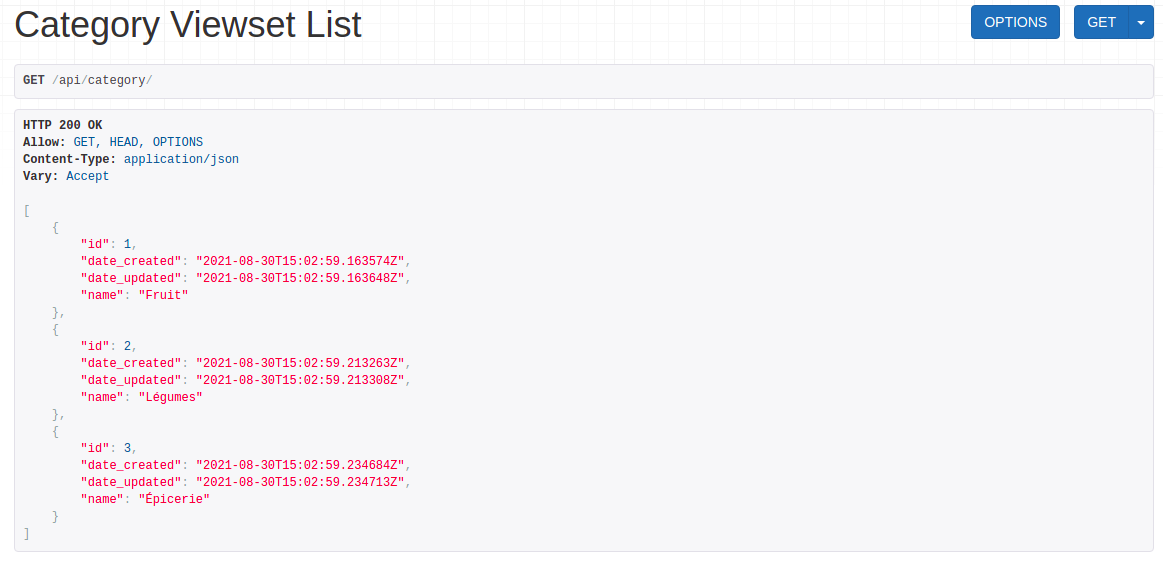
\includegraphics[width=10cm]{images/image08.png}
\end{center}

Remarquez que des composants sont réutilisés plusieurs fois : un composant {\color{monOrange}Article} pour les deux articles affichés et un composant {\color{monOrange}Item} pour les trois informations affichées à droite.

\subsection{Syntaxe des composants}
Nous avons vu que les fichiers des composants étaient écrits en {\color{monOrange}PascalCase} et devaient terminer par l'extension {\color{monOrange}.vue}.

Cette syntaxe permet de créer des composants monofichiers ({\color{monOrange}SFCs}) avec une partie {\color{monOrange}template}, une partie script et une partie style. Cette syntaxe est rendue possible grâce à {\color{monOrange}Vite} et plus précisément au {\color{monOrange}plugin Vue} qui va transformer les {\color{monOrange}SFCs} lors d'une étape de {\color{monOrange}build}.

\subsection{Utiliser des composants enfants}
Pour utiliser un composant enfant dans un composant parent, il suffit d'importer le ou les composants dans la partie {\color{monOrange}script} et de les utiliser dans la partie {\color{monOrange}template}.

La syntaxe recommandée pour utiliser un composant enfant est {\tt <ComposantEnfant />}. Cela permet de distinguer en un coup d'œil les composants {\color{monOrange}Vue.js} des éléments HTML. Dans notre exemple, nous aurions par exemple dans le composant {\color{monOrange}Root }:
\begin{minted}[
mathescape,
framesep=2mm,
baselinestretch=1.2,
%fontsize=\footnotesize,
bgcolor=LightGray,
%linenos
]{html}
<script setup>
import Header from './Header.vue';
import Main from './Main.vue';
import Aside from './Aside.vue';
</script>

<template>
  <Header />
  <Main />
  <Aside />
</template>
\end{minted}
Les composants sont automatiquement exportés grâce à l'utilisation de l'attribut {\color{monOrange}setup} sur les balises {\color{monOrange}scripts}. Aussi, il n'y a rien à exporter manuellement dans les composants enfants.

%Exemple exécutable de la vidéo
%Vous pouvez directement utiliser ce code exécutable. N'hésitez pas à l'ouvrir dans un nouvel onglet pour le modifier ou mieux voir :

\section{Composants locaux et globaux}
\subsection{Enregistrement des composants}
Tous les composants {\color{monOrange}Vue.js} ont besoin d'être enregistrés pour que {\color{monOrange}Vue} puisse savoir où les chercher lorsque vous les utilisez. Il est possible d'enregistrer les composants soit localement, soit globalement.

\subsection{Enregistrement global}
Pour enregistrer des composants globalement, il faut modifier le fichier {\color{monOrange}main.ts} et utiliser la méthode {\color{monOrange}component()} sur l'instance retournée par {\color{monOrange}createApp()} :
\begin{minted}[
mathescape,
framesep=2mm,
baselinestretch=1.2,
%fontsize=\footnotesize,
bgcolor=LightGray,
%linenos
]{javascript}
import { createApp } from 'vue';
import App from './App.vue';
import ComponentA from './'ComponentA'.vue';
import ComponentB from './'ComponentB'.vue';
import ComponentC from './'ComponentC'.vue';


const app = createApp(App);

app
  .component('ComponentA', ComponentA)
  .component('ComponentB', ComponentB)
  .component('ComponentC', ComponentC)

app.mount('#app');
\end{minted}
Le premier argument est le nom à donner au composant dans l'application et le deuxième argument est le composant lui-même qui est importé depuis le fichier où il est situé. Ces composants peuvent être utilisés par n'importe quel composant de votre application, d'où le nom d'enregistrement global. Il existe cependant deux problèmes à l'enregistrement global :
\begin{enumerate}
\item  Le {\color{monOrange}tree-shaking} n'est pas possible. Le {\color{monOrange}tree-shaking} permet d'enlever automatiquement du {\color{monOrange}build} les composants qui ne sont pas utilisés.
\item La relation entre les composants devient difficilement maintenable. Le fait de déclarer tous les composants au même endroit rend difficile le fait de retrouver un composant enfant utilisé dans un composant. Nous n'avons en effet pas accès au chemin dans la partie {\color{monOrange}script} du composant parent. Il faut regarder pour chaque composant dans le fichier {\color{monOrange}main.ts} où il est déclaré. Pour les grandes applications, cela devient rapidement illisible.
\end{enumerate}
\subsection{Enregistrement local}
Les composants enregistrés localement sont disponibles uniquement dans le composant qui les importe. Il est donc nécessaire d'importer le même composant enfant dans tous les composants parents qui l'utilisent. Mais c'est beaucoup plus clair de cette manière : vous savez en un coup d'œil quels composants enfants sont utilisés par un composant en regardant ses imports.

Avant l'apparition de la syntaxe {\color{monOrange}script setup} dans la version {\color{monOrange}3.2}, les composants enregistrés localement devaient être enregistrés comme ceci :
\begin{minted}[
mathescape,
framesep=2mm,
baselinestretch=1.2,
%fontsize=\footnotesize,
bgcolor=LightGray,
%linenos
]{javascript}
import ComponentA from './ComponentA.vue'

export default {
  components: {
    ComponentA
  },
  setup() {
    // ...
  }
}
\end{minted}
Aujourd'hui c'est beaucoup plus simple :
\begin{minted}[
mathescape,
framesep=2mm,
baselinestretch=1.2,
%fontsize=\footnotesize,
bgcolor=LightGray,
%linenos
]{html}
<script setup>
import ComponentA from './ComponentA.vue'
</script>
\end{minted}
Le composant est automatiquement enregistré localement !

%Exemple exécutable de la vidéo
%Vous pouvez directement utiliser ce code exécutable. N'hésitez pas à l'ouvrir dans un nouvel onglet pour le modifier ou mieux voir :


\section{Les props}
\subsection{Communications entre les composants}
Nous avons vu dans les chapitres précédents comment utiliser des composants : comment les définir, comment les instancier, comment fonctionne une architecture en arbre de composants monofichiers etc. Mais il reste un problème : comment faire passer des données le long de notre arbre de composants ?

Comment communiquer des données d'un composant parent vers un composant enfant et d'un composant enfant vers un composant parent ? C'est ce que nous allons voir maintenant.

\subsection{Utilisation des attributs {\color{monOrange}props}}
Vous pouvez passer des valeurs dans le sens parent $\to$ enfant en utilisant des {\color{monOrange}props}. Nous allons partir d'un exemple simple pour bien comprendre.

Supposons que nous avons deux composants : {\color{monOrange}Parent.vue} et {\color{monOrange}Enfant.vue}. Voici notre composant {\color{monOrange}Enfant.vue} :
\begin{minted}[
mathescape,
framesep=2mm,
baselinestretch=1.2,
%fontsize=\footnotesize,
bgcolor=LightGray,
%linenos
]{html}
<template>
  <h3>{{ prenom }}</h3>
</template>

<script setup>
const props = defineProps(['prenom']);
console.log(props.prenom);
</script>
\end{minted}
La fonction {\color{monOrange}defineProps()} permet de déclarer les propriétés récupérées sur le composant enfant depuis le composant parent. Ici nous récupérons {\color{monOrange}prenom}. Elles sont directement utilisables sur le {\color{monOrange}template} et nous pouvons les récupérer dans la partie {\color{monOrange}script} en déclarant une variable {\color{monOrange}props}. Dans notre composant {\color{monOrange}Parent.vue} :
\begin{minted}[
mathescape,
framesep=2mm,
baselinestretch=1.2,
%fontsize=\footnotesize,
bgcolor=LightGray,
%linenos
]{html}
<template>
    <Enfant prenom="Paul" />
</template>

<script>
import Enfant from './Enfant.vue';
</script>
\end{minted}
Nous passons de la donnée de manière unidirectionnelle de {\color{monOrange}Parent.vue} vers {\color{monOrange}Enfant.vue}. Pour ce faire, nous utilisons simplement un attribut {\color{monOrange}prenom} et lui donnons pour l'instant une valeur fixe. Nous pouvons définir n'importe quel attribut personnalisé de cette manière, du moment qu'il n'entre pas en collision avec le nom de d'un attribut HTML natif (par exemple {\color{monOrange}style}).

Il ne faut jamais modifier une {\color{monOrange}props} dans un composant enfant. Nous verrons comment passer des données du composant enfant vers le composant parent.

\subsection{Utilisation d'une liaison dynamique}
Nous souhaitons maintenant que les données que nous passons soient liées de manière dynamique. C'est-à-dire que nous voulons que le composant enfant puisse recevoir la nouvelle valeur de l'attribut que nous lui passons depuis le composant parent lorsqu'elle change. Pour ce faire il suffit d'utiliser la directive {\color{monOrange}v-bind} :
\begin{minted}[
mathescape,
framesep=2mm,
baselinestretch=1.2,
%fontsize=\footnotesize,
bgcolor=LightGray,
%linenos
]{html}
<template>
    <Enfant :prenom="prenom" />
</template>

<script>
import Enfant from './Enfant.vue';
import { ref } from 'vue';

const prenom = ref('Jean');
</script>
\end{minted}
Nous définissons une variable réactive sur notre composant parent {\color{monOrange}prenom}. Nous utilisons la directive {\color{monOrange}v-bind} pour lier cette propriété réactive à la {\color{monOrange}prop} passée au composant enfant.

\subsection{Typage des propriétés props}
Nous avons vu que nous pouvions utiliser sur le composant enfant une fonction {\color{monOrange}defineProps()} et lui passer un tableau avec le nom des {\color{monOrange}props} que nous passons depuis le composant parent. Pour plus de sécurité lors du développement, nous pouvons typer les propriétés sur {\color{monOrange}props} afin de définir le type de valeur attendu.

Les types possibles sont {\color{monOrange}String, Number, Boolean, Array, Object, Function, Date} et {\color{monOrange}Symbol}. Par exemple, pour notre attribut {\color{monOrange}prenom} nous souhaitons que ce dernier soit de type {\color{monOrange}String}. Nous allons donc typer la {\color{monOrange}props} en utilisant un objet au lieu d'un tableau dans la fonction {\color{monOrange}defineProps()} sur le composant enfant :
\begin{minted}[
mathescape,
framesep=2mm,
baselinestretch=1.2,
%fontsize=\footnotesize,
bgcolor=LightGray,
%linenos
]{html}
…
const props = defineProps({
  prenom: String,
});
</script>
...
\end{minted}
Si la valeur de {\color{monOrange}prenom} passée n'est pas de type {\color{monOrange}String}, alors {\color{monOrange}Vue} nous affichera un message d'erreur dans la console JavaScript de notre navigateur. En outre, grâce à {\color{monOrange}Volar} et {\color{monOrange}TypeScript} nous aurons l'auto-complétion des {\color{monOrange}props} et le contrôle des types. Vous pouvez également typer une propriété en permettant plusieurs types, par exemple {\color{monOrange}[String, Number]} :
\begin{minted}[
mathescape,
framesep=2mm,
baselinestretch=1.2,
%fontsize=\footnotesize,
bgcolor=LightGray,
%linenos
]{html}
<script>
//…
const props = defineProps({
  prenom: [String, Number],
});
</script>
...
\end{minted}
Dans ce cas, cette propriété pourra être une chaîne de caractères ou un nombre.

\subsubsection{Utilisation d'un objet pour plus d'options de type}
Vous pouvez également utiliser un objet pour accéder à plus d'options de typage et à des validateurs : Vous pouvez rendre un attribut obligatoire avec {\color{monOrange}required} :
\begin{minted}[
mathescape,
framesep=2mm,
baselinestretch=1.2,
%fontsize=\footnotesize,
bgcolor=LightGray,
%linenos
]{html}
<script>
//…
const props = defineProps({
  prenom: {
        type: String,
        required: true
    }
});
</script>
\end{minted}
Vous pouvez attribuer une valeur par défaut à un attribut :
\begin{minted}[
mathescape,
framesep=2mm,
baselinestretch=1.2,
%fontsize=\footnotesize,
bgcolor=LightGray,
%linenos
]{html}
<script>
//…
const props = defineProps({
  prenom: {
        type: String,
        required: true,
        default: 'Jean'
    }
});
</script>
\end{minted}

\subsubsection{Valeur par défaut des propriétés {\color{monOrange}props} de type {\color{monOrange}Object}}
Si vous souhaitez passer un objet comme donnée depuis un composant parent à un composant enfant, vous pouvez utiliser les mêmes fonctionnalités, cependant vous devrez effectuer une adaptation. La raison est toujours la même : les objets et les tableaux sont passés par référence et non par valeur en JavaScript. Il est donc nécessaire d'utiliser des fonctions pour fabriquer de nouveaux objets pour chaque instance. Dans le cas contraire, le même objet serait utilisé pour toutes les instances d'un composant enfant. Il faut donc utiliser une fonction pour définir une valeur par défaut à notre objet :
\begin{minted}[
mathescape,
framesep=2mm,
baselinestretch=1.2,
%fontsize=\footnotesize,
bgcolor=LightGray,
%linenos
]{javascript}
titre: {
      type: Object,
      default() {
        return { title: 'Mon super titre' }
      }
},
\end{minted}

\subsection{Nommage des {\color{monOrange}props}}
Si vos noms de {\color{monOrange}props} sont longs, il est recommandé d'utiliser côté composant parent le {\color{monOrange}kebab-case} :
\begin{minted}[
mathescape,
framesep=2mm,
baselinestretch=1.2,
%fontsize=\footnotesize,
bgcolor=LightGray,
%linenos
]{html}
<Enfant une-longue-prop="test" />
\end{minted}
Côté composant enfant il faut utiliser le {\color{monOrange}camelCase} pour récupérer la {\color{monOrange}prop} :
\begin{minted}[
mathescape,
framesep=2mm,
baselinestretch=1.2,
%fontsize=\footnotesize,
bgcolor=LightGray,
%linenos
]{html}
<script setup lang="ts">
defineProps({
  uneLongueProp: String
})
</script>
\end{minted}

\subsection{Passer des types statiques autres que des chaînes de caractères}
Pour passer des {\color{monOrange}props} statiques autre que des chaînes de caractères, il faut utiliser {\color{monOrange}v-bind} :
\begin{minted}[
mathescape,
framesep=2mm,
baselinestretch=1.2,
%fontsize=\footnotesize,
bgcolor=LightGray,
%linenos
]{html}
<Enfant :nombre="42" :booleen="false" />
\end{minted}
De même pour les tableaux ou les objets :
\begin{minted}[
mathescape,
framesep=2mm,
baselinestretch=1.2,
%fontsize=\footnotesize,
bgcolor=LightGray,
%linenos
]{html}
<Enfant :tableau="[5, 2, 1]" />
\end{minted}

\subsection{Passer un objet de {\color{monOrange}props}}
Si vous avez de nombreuses {\color{monOrange}props} vous pouvez passer un objet en utilisant la notation longue de {\color{monOrange}v-bind} :
\begin{minted}[
mathescape,
framesep=2mm,
baselinestretch=1.2,
%fontsize=\footnotesize,
bgcolor=LightGray,
%linenos
]{html}
<script>
const objet = {
  id: 1,
  title: 'Un titre'
};
</script>

<template>
  <Enfant v-bind="objet" />
</template>
\end{minted}

%Exemple exécutable de la vidéo
%Vous pouvez directement utiliser ce code exécutable. N'hésitez pas à l'ouvrir dans un nouvel onglet pour le modifier ou mieux voir :

%%%%%%%%%%%%%%%%%%%%%%%%%%%%%%%%%%%%%%%%%%%%%%%%%%%%%%%%%%%

\section{Validation des props et utilisation de TypeScript}
\subsection{Utilisation des validateurs}
Vous pouvez créer un validateur personnalisé pour la valeur de votre attribut. Celui-ci doit être une fonction prenant en paramètre la valeur de l'attribut et doit tester cette valeur puis retourner un booléen :
\begin{minted}[
mathescape,
framesep=2mm,
baselinestretch=1.2,
%fontsize=\footnotesize,
bgcolor=LightGray,
%linenos
]{javascript}
defineProps({
  title: {
    type: String,
    validator(value) {
      return value.length > 2;
    }
  }
}
\end{minted}

\subsection{Notation raccourcie pour les booléens}
Les {\color{monOrange}props} de type booléen ont une notation raccourcie. Par exemple si vous définissez sur le composant enfant :
\begin{minted}[
mathescape,
framesep=2mm,
baselinestretch=1.2,
%fontsize=\footnotesize,
bgcolor=LightGray,
%linenos
]{javascript}
defineProps({
  available: Boolean
})
\end{minted}
Vous pouvez directement passer le {\color{monOrange}prop} de cette manière côté parent :
\begin{minted}[
mathescape,
framesep=2mm,
baselinestretch=1.2,
%fontsize=\footnotesize,
bgcolor=LightGray,
%linenos
]{html}
<Enfant available />
\end{minted}

\subsection{Les génériques TypeScript}
Les génériques sont une fonctionnalité de {\color{monOrange}TypeScript} permettant une grande flexibilité combinée à une sécurité du typage. Lorsque vous débutez avec {\color{monOrange}TypeScript} vous rencontrez deux travers :
\begin{enumerate}
\item Trop typer en {\color{monOrange}any}. Cela vous donne une grande flexibilité mais vous perdez totalement en sécurité et en autocomplétion.

\item Tout typer correctement sans utiliser de génériques. Cela conférera à votre code la sécurité et l'autocomplétion permise par le typage fort mais vous perdrez en flexibilité, ce qui provoque beaucoup de duplications et de lourdes dans votre code.
\end{enumerate}


En résumé, l'objectif des génériques est de permettre d'utiliser des éléments (fonctions, classes, interfaces etc) qui peuvent fonctionner avec une diversité de types tout en conservant l'utilité de {\color{monOrange}TypeScript}, à savoir la sécurité et l'autocomplétion. Nous allons donner deux exemples de types génériques utilisés nativement.

\subsubsection{Le typage des tableaux}
Nous avons vu comment typer des tableaux pour qu'ils n'acceptent qu'un seul type en faisant :
\begin{minted}[
mathescape,
framesep=2mm,
baselinestretch=1.2,
%fontsize=\footnotesize,
bgcolor=LightGray,
%linenos
]{javascript}
const tableau: string[] = ['Des', 'chaînes', 'de', 'caractères'];
\end{minted}
La notation alternative est :
\begin{minted}[
mathescape,
framesep=2mm,
baselinestretch=1.2,
%fontsize=\footnotesize,
bgcolor=LightGray,
%linenos
]{javascript}
const tableau: Array<string> = ['Des', 'chaînes', 'de', 'caractères'];
\end{minted}
Si vous passez la souris sur {\color{monOrange}Array} vous verrez {\tt interface Array<T>}. Cela signifie que {\color{monOrange}Array} prend en fait un argument appelé {\color{monOrange}T} par convention pour type. L'interface {\tt Array<T>} utilise donc un type générique, nous pouvons passer n'importe quel type comme argument et le tableau devra comporter le type défini. Exemple avec une union de types :
\begin{minted}[
mathescape,
framesep=2mm,
baselinestretch=1.2,
%fontsize=\footnotesize,
bgcolor=LightGray,
%linenos
]{javascript}
const tableau: Array<string | boolean> = ['Des', 'chaînes', 'de', 'caractères', true];
\end{minted}
Autre exemple en utilisant une {\color{monOrange}interface} :
\begin{minted}[
mathescape,
framesep=2mm,
baselinestretch=1.2,
%fontsize=\footnotesize,
bgcolor=LightGray,
%linenos
]{javascript}
interface User {
  name: string;
}

const tableau: Array<User> = [{name: 'Paul'}, {name: 'Jean'}];
\end{minted}
Vous commencez à percevoir l'idée de générique : nous passons en argument n'importe quel type à l'interface {\tt Array<T>}, et {\color{monOrange}TypeScript} nous obligera à le respecter.

\subsubsection{Autre exemple : les promesses}
Prenons un exemple avec une promesse :
\begin{minted}[
mathescape,
framesep=2mm,
baselinestretch=1.2,
%fontsize=\footnotesize,
bgcolor=LightGray,
%linenos
]{javascript}
let condition: boolean;

const promesse = new Promise((resolve, reject) => {
  if (condition) {
    resolve(42)
  } else {
    reject('Erreur');
  }
});
\end{minted}
Dans {\color{monOrange}VS Code}, si vous passez la souris sur la constante, vous aurez {\tt Promise<unknown>}. Ici, {\color{monOrange}TypeScript} utilise également un générique pour typer la valeur remboursée par la promesse. Autrement dit, il utilise une {\tt interface Promise<T>}, et donc les génériques. Ici, il ne peut pas détecter le type par inférence et préciser donc que la valeur retournée est de type inconnu : {\color{monOrange}unknown}. En revanche, si nous passons un argument, {\color{monOrange}TypeScript} saura que les valeurs retournées dans les promesses seront du type spécifié :
\begin{minted}[
mathescape,
framesep=2mm,
baselinestretch=1.2,
%fontsize=\footnotesize,
bgcolor=LightGray,
%linenos
]{javascript}
let condition: boolean;

const promesse: Promise<number | string> = new Promise((resolve, reject) => {
  if (condition) {
    resolve(42)
  } else {
    reject('Erreur');
  }
});
\end{minted}
Ici, nous indiquons à {\color{monOrange}TypeScript} les valeurs retournées dans la promesse ce qui permet la sécurité et l'autocomplétion. A savoir que si vous essayez d'utiliser par exemple une méthode disponible sur les tableaux ou les objets sur la valeur de retour, {\color{monOrange}TypeScript} vous renverra une erreur. Par exemple :
\begin{minted}[
mathescape,
framesep=2mm,
baselinestretch=1.2,
%fontsize=\footnotesize,
bgcolor=LightGray,
%linenos
]{javascript}
let condition: boolean;

const promesse: Promise<number | string> = new Promise((resolve, reject) => {
  if (condition) {
    resolve(42)
  } else {
    reject('Erreur');
  }
});

promesse.then((val) => {
  val.map()
})
\end{minted}
Ici, vous aurez une erreur {\color{red}Property 'map' does not exist on type 'string | number'}.

De même, {\color{monOrange}VS Code} vous proposera en autocomplétion sur {\color{monOrange}val} les méthodes et propriétés partagées par les types nombre et chaînes de caractères. Si vous mettiez {\tt Promise<any>}, {\color{monOrange}TypeScript} ne feriez plus de contrôle sur les valeurs de retour, sur les méthodes que l'on tente d'accéder etc.
\begin{minted}[
mathescape,
framesep=2mm,
baselinestretch=1.2,
%fontsize=\footnotesize,
bgcolor=LightGray,
%linenos
]{javascript}
let condition: boolean;

const promesse: Promise<any> = new Promise((resolve, reject) => {
  if (condition) {
    resolve(42)
  } else {
    reject('Erreur');
  }
});

promesse.then((val) => {
  val.map()
})
\end{minted}
Ici aucun problème lors de la compilation et dans {\color{monOrange}VS Code}, pourtant l'accès à la méthode {\color{monOrange}map()} provoquera une erreur lors de l' ;exécution.

\subsection{Utilisation de {\color{monOrange}TypeScript} avec les {\color{monOrange}props}}
Vous pouvez également utiliser la syntaxe {\color{monOrange}TypeScript} au lieu de passer un objet à {\color{monOrange}props}, dans ce cas on utilise un type générique
\begin{minted}[
mathescape,
framesep=2mm,
baselinestretch=1.2,
%fontsize=\footnotesize,
bgcolor=LightGray,
%linenos
]{html}
<script setup lang="ts">
defineProps<{
  prenom?: string
  age?: number
}>()
</script>
\end{minted}
Remarquez que nous utilisons un type générique et non plus un argument passé à {\color{monOrange}defineProps()}. Le plus souvent nous utiliserons des {\color{monOrange}interfaces} de cette manière ;
\begin{minted}[
mathescape,
framesep=2mm,
baselinestretch=1.2,
%fontsize=\footnotesize,
bgcolor=LightGray,
%linenos
]{html}
<script setup lang="ts">
interface Props {
  prenom: string
  age?: number
}

const props = defineProps<Props>()
</script>
\end{minted}

%Exemple exécutable de la vidéo
%Vous pouvez directement utiliser ce code exécutable. N'hésitez pas à l'ouvrir dans un nouvel onglet pour le modifier ou mieux voir :

%%%%%%%%%%%%%%%%%%%%%%%%%%%%%%%%%%%%%%%%%%%%%%%%%%%%%%%%%%%%%%

\section{Les événements}
\subsection{Communiquer des composants enfants vers les composants parents}
Nous allons maintenant nous intéresser au sens de communication inverse : des composants enfants vers les composants parents. Pour communiquer dans ce sens, nous utilisons les événements personnalisés. Il faut déclarer l'événement sur le composant enfant et l'écouter sur le composant parent. Dans le {\color{monOrange}template} du composant parent, nous enregistrons l'écoute d'un événement personnalisé avec la directive {\color{monOrange}v-on} :
\begin{minted}[
mathescape,
framesep=2mm,
baselinestretch=1.2,
%fontsize=\footnotesize,
bgcolor=LightGray,
%linenos
]{javascript}
<Enfant
  ...
  @un-evenement="gestionnaire"
 />
\end{minted}
Dans la partie {\color{monOrange}script} du composant enfant, nous déclarons l'événement avec {\color{monOrange}defineEmits()} :
\begin{minted}[
mathescape,
framesep=2mm,
baselinestretch=1.2,
%fontsize=\footnotesize,
bgcolor=LightGray,
%linenos
]{javascript}
const emit = defineEmits(['un-evenement']);
\end{minted}
Nous pouvons émettre l'événement côté {\color{monOrange}script} en utilisant :
\begin{minted}[
mathescape,
framesep=2mm,
baselinestretch=1.2,
%fontsize=\footnotesize,
bgcolor=LightGray,
%linenos
]{javascript}
emit('un-evenement');
\end{minted}

\subsection{Émettre des événements sans utiliser defineEmits()}
Côté composant enfant, vous pouvez émettre directement des événements sans passer par {\color{monOrange}defineEmits()}, en utilisant {\tt \$emit()} dans le {\color{monOrange}template} :
\begin{minted}[
mathescape,
framesep=2mm,
baselinestretch=1.2,
%fontsize=\footnotesize,
bgcolor=LightGray,
%linenos
]{html}
<button @click="$emit('unEvenement')">Cliquer</button>
\end{minted}
Il faut utiliser le {\color{monOrange}camelCase} pour le nom de l'événement. Côté composant, parent, cela ne change pas, nous utilisons {\color{monOrange}v-on} pour écouter l'événement écrit en {\color{monOrange}kebab-case} :
\begin{minted}[
mathescape,
framesep=2mm,
baselinestretch=1.2,
%fontsize=\footnotesize,
bgcolor=LightGray,
%linenos
]{html}
<Enfant @un-evenement="gestionnaire" />
\end{minted}
\subsection{Passer des arguments}
Vous pouvez passer des arguments lors de l'émission d'un événement. Il suffit de les passer en argument dans le composant enfant :
\begin{minted}[
mathescape,
framesep=2mm,
baselinestretch=1.2,
%fontsize=\footnotesize,
bgcolor=LightGray,
%linenos
]{html}
<button @click="$emit('unEvenement', 42, 'unEvenement')">Cliquer</button>
\end{minted}
Côté composant parent vous pouvez les récupérer dans le gestionnaire d'événement :
\begin{minted}[
mathescape,
framesep=2mm,
baselinestretch=1.2,
%fontsize=\footnotesize,
bgcolor=LightGray,
%linenos
]{html}
<Enfant @un-evenement="gestionnaire" />
\end{minted}
Par exemple :
\begin{minted}[
mathescape,
framesep=2mm,
baselinestretch=1.2,
%fontsize=\footnotesize,
bgcolor=LightGray,
%linenos
]{javascript}
function gestionnaire(arg1, arg2) {
  console.log(arg1, arg2);
}
\end{minted}

\subsection{Validation des évenements}
Comme pour les {\color{monOrange}props}, il est possible de valider les événements, même si c'est assez peu utilisé. Par exemple :
\begin{minted}[
mathescape,
framesep=2mm,
baselinestretch=1.2,
%fontsize=\footnotesize,
bgcolor=LightGray,
%linenos
]{html}
<script setup>
const emit = defineEmits({
  submit: ({ email, password }) => {
    if (email && password) {
      return true;
    } else {
      return false;
    }
  }
})

function submitForm(email, password) {
  emit('submit', { email, password })
}
</script>
\end{minted}
Ici notre événement {\color{monOrange}submit} prend en argument un objet  {\color{monOrange}\{ email, password \}}. La fonction de validation définie dans {\color{monOrange}defineEmits()} reçoit cet argument dans une fonction de rappel. Cette fonction de rappel retourne {\color{monOrange}true} si l'événement est valide et false sinon. Ici, il est considéré que l'événement est valide si {\color{monOrange}email} et {\color{monOrange}password} sont définis.

{\em Nous ne détaillerons pas davantage car ce type de validation est très rarement utilisé, et seulement en développement. Nous verrons comment valider des formulaires plus tard}.

\subsection{Syntaxe recommandée : utilisation de {\color{monOrange}defineEmits} avec {\color{monOrange}TypeScript}}
Dans la suite de la formation nous utiliserons ce qui est recommandé par {\color{monOrange}Vue} officiellement : déclarer explicitement les événements utilisés avec {\color{monOrange}defineEmits()} en utilisant {\color{monOrange}TypeScript}. Comme pour les {\color{monOrange}props}, il suffit de passer un générique à la fonction pour déclarer les types des événements utilisés :
\begin{minted}[
mathescape,
framesep=2mm,
baselinestretch=1.2,
%fontsize=\footnotesize,
bgcolor=LightGray,
%linenos
]{javascript}
const emit = defineEmits<{
  (e: 'change', id: number): void;
  (e: 'update', value: string): void;
}>()
\end{minted}

Ici nous déclarons un événement {\color{monOrange}change} qui contient un argument {\color{monOrange}id} de type {\color{monOrange}number} et un événement {\color{monOrange}update} qui contient un argument {\color{monOrange}value} de type chaîne de caractères.

%Exemple exécutable de la vidéo
%Vous pouvez directement utiliser ce code exécutable. N'hésitez pas à l'ouvrir dans un %nouvel onglet pour le modifier ou mieux voir :

%%%%%%%%%%%%%%%%%%%%%%%%%%%%%%%%%%%%%%%%%%%%%%%%%%%%%%

\section{Le cycle de vie d'un composant}
\subsection{Le cycle de vie des composants}
Les composants {\color{monOrange}Vue.js} passent par différents stades de leur initialisation, à l'affichage sur le DOM, puis à leurs mises à jour et enfin à leur destruction et enlèvement du DOM.
\begin{center}
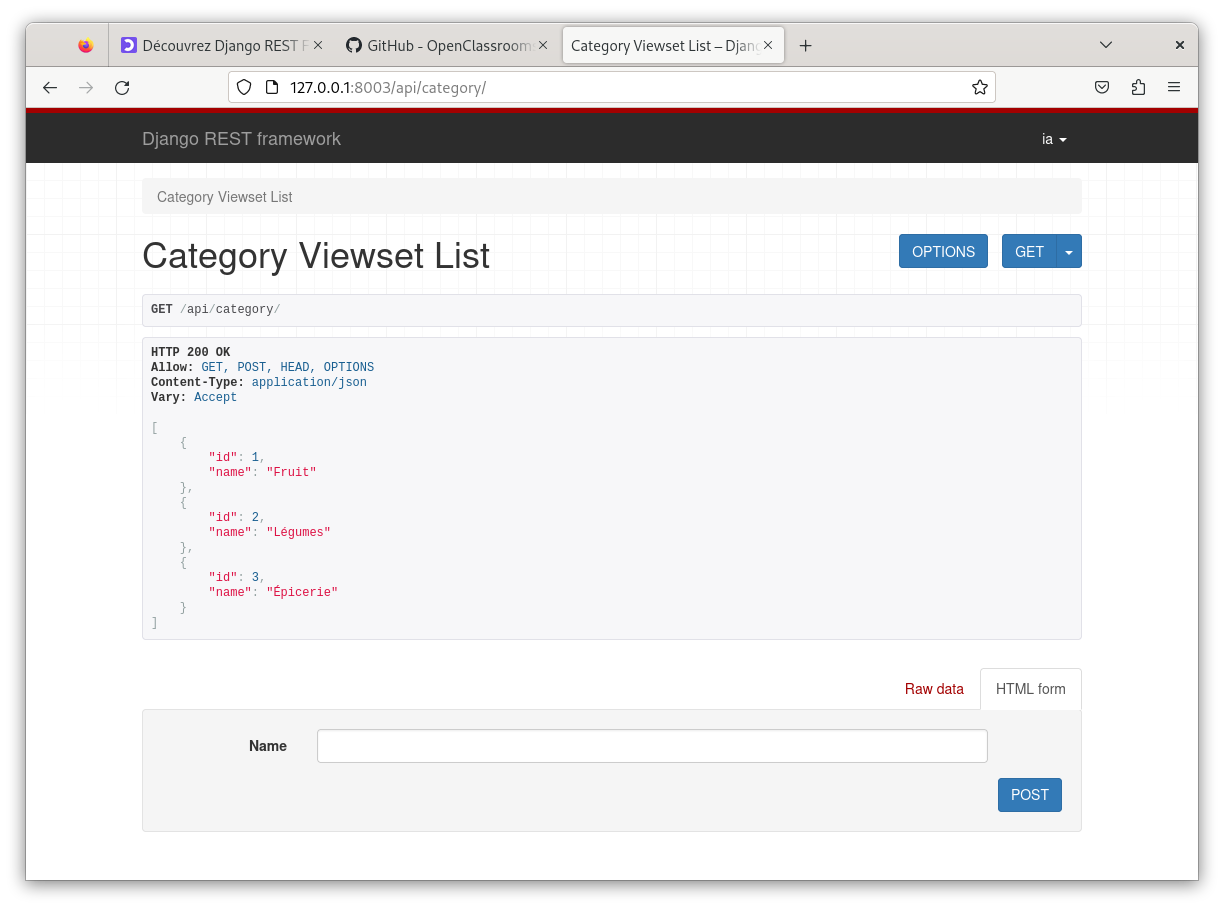
\includegraphics[width=10cm]{images/image09.png}
\end{center}

Lors de ces étapes de leur cycle, des fonctions peuvent être appelées pour effectuer des tâches. Ces fonctions sont appelées des {\color{monOrange}lifecycle hooks} (littéralement des accroches du cycle de vie).

Les {\color{monOrange}hooks} les plus utilisés sont :
\begin{itemize}
\item {\color{monOrange}onMounted()} : appelée juste après que le composant soit monté (donc lorsque le composant et ses descendants sont affichés sur le DOM).

\item {\color{monOrange}onUpdated()} : appelée lorsque le composant a été mis à jour et qu'un changement sur le DOM a été effectué.

\item {\color{monOrange}onUnmounted()} : appelée après que tous les effets réactifs aient été stoppés et lorsque le composant va être retiré du DOM. On l'utilise pour faire des opérations de nettoyage.
\end{itemize}
Les autres hooks sont :
\begin{itemize}
\item {\color{monOrange}onBeforeMount()} : qui est appelée lorsque le composant a été initialisé (notamment son état réactif) mais lorsqu'aucun élément n'a encore été créé sur le DOM.

\item {\color{monOrange}onBeforeUpdate()} : appelée juste avant que le composant n'ait mis à jour son DOM suite à un changement de son état réactif.

\item {\color{monOrange}onBeforeUnmount()} : appelée lorsque le composant est encore fonctionnel mais va être détruit.

\item {\color{monOrange}onErrorCaptured()} : appelée lorsqu'une erreur se propage depuis un composant enfant.

\end{itemize}

Nous verrons les autres {\color{monOrange}hooks} qui ont des cas avancés d'utilisations : {\color{monOrange} onRenderTracked(), onRenderTriggered(), onActivated(), onDeactivated() et onServerPrefetch()}. Ils sont relatifs au développement, aux composants {\color{monOrange}keepalive} et au {\color{monOrange}SSR}.

\subsection{Utiliser un {\color{monOrange}hook}}
Pour utiliser un hook c'est très simple, il suffit d'utiliser la fonction de {\color{monOrange}hook} adéquate et de lui passer une fonction de rappel contenant les tâches à exécuter lorsque l'état est atteint :
\begin{minted}[
mathescape,
framesep=2mm,
baselinestretch=1.2,
%fontsize=\footnotesize,
bgcolor=LightGray,
%linenos
]{html}
<script setup>
import { onMounted } from 'vue'

onMounted(() => {
  console.log('Le composant est présent sur le DOM.')
})
</script>
\end{minted}

%Exemple exécutable de la vidéo
%Vous pouvez directement utiliser ce code exécutable. N'hésitez pas à l'ouvrir dans un nouvel onglet pour le modifier ou mieux voir :

%%%%%%%%%%%%%%%%%%%%%%%%%%%%%%%%%%%%%%%%%%%%%%%%%%%%%%%%%%%%%%%%

\section{Les références de template}
\subsection{Les références de {\color{monOrange}templates}}
Parfois, vous voudrez accéder directement à un élément du DOM pour effectuer des opérations particulières. Dans ce cas, {\color{monOrange}Vue.js} propose de créer une référence côté {\color{monOrange}template} avec l'attribut {\color{monOrange}ref }:
\begin{minted}[
mathescape,
framesep=2mm,
baselinestretch=1.2,
%fontsize=\footnotesize,
bgcolor=LightGray,
%linenos
]{html}
<input ref="input">
\end{minted}
L'élément du DOM référencé devient alors accessible depuis le {\color{monOrange}script} :
\begin{minted}[
mathescape,
framesep=2mm,
baselinestretch=1.2,
%fontsize=\footnotesize,
bgcolor=LightGray,
%linenos
]{html}
<script setup>
import { ref, onMounted } from 'vue';

const input = ref(null);

onMounted(() => {
  input.value.focus();
})
</script>
\end{minted}
Le code précédent récupère le champ en utilisant la référence déclarée et va ensuite utiliser la méthode {\color{monOrange}focus()} permettant de cibler l'élément. Nous sommes sûr que le champ a été créé sur le DOM, car nous utilisons le {\color{monOrange}hook onMounted()} que nous avons vu dans la leçon précédente. Nous sommes obligé d'utiliser le {\color{monOrange}hook onMounted()} car nous manipulons un élément du DOM et il faut donc que celui-ci soit créé sur le DOM avant que nous y accédions.

\subsection{Utilisation des {\color{monOrange}refs} avec {\color{monOrange}v-for}}
Lorsque nous utilisons {\color{monOrange}ref} avec la directive {\color{monOrange}v-for}, il faut que la référence côté {\color{monOrange}script} contienne un tableau qui contiendra les éléments :
\begin{minted}[
mathescape,
framesep=2mm,
baselinestretch=1.2,
%fontsize=\footnotesize,
bgcolor=LightGray,
%linenos
]{html}
<script setup>
import { ref, onMounted } from 'vue';

const list = ref([1, 2, 3, 4]);

const itemRefs = ref([]);

onMounted(() => console.log(itemRefs.value));
</script>

<template>
  <ul>
    <li v-for="item in list" ref="itemRefs">
      {{ item }}
    </li>
  </ul>
</template>
\end{minted}

\subsection{Utilisation des {\color{monOrange}refs} avec des composants}
L'attribut {\color{monOrange}ref} peut également être utilisé sur les composants enfants. Par exemple :
\begin{minted}[
mathescape,
framesep=2mm,
baselinestretch=1.2,
%fontsize=\footnotesize,
bgcolor=LightGray,
%linenos
]{html}
<script setup>
import { ref, onMounted } from 'vue';
import Enfant from './Enfant.vue';

const enfant = ref(null);

onMounted(() => {
  // enfant.value contient l'élément Enfant
});
</script>

<template>
  <Enfant ref="enfant" />
</template>
\end{minted}
Attention ! Il n'est pas possible par défaut d'accéder aux propriétés des composants enfants en utilisant une référence car ces propriétés sont privées par défaut. Il faut exposer, avec {\color{monOrange}defineExpose()}, les propriétés auxquelles vous souhaitez accéder dans le composant parent, depuis le composant enfant :
\begin{minted}[
mathescape,
framesep=2mm,
baselinestretch=1.2,
%fontsize=\footnotesize,
bgcolor=LightGray,
%linenos
]{html}
<script setup>
import { ref } from 'vue';

const a = 21;
const b = ref(42);

defineExpose({
  a,
  b
})
</script>
\end{minted}
En utilisant {\color{monOrange}defineExpose()} nous rendons accessibles les deux variables depuis le composant parent qui peut ensuite les récupérer sur {\color{monOrange}enfant.value : enfant.value.a et enfant.value.b}.

\subsection{Utilisation de {\color{monOrange}TypeScript}}
Bien entendu, il faut également typer avec {\color{monOrange}TypeScript} les références. Nous allons voir comment le faire.

\subsubsection{Typer les références contenant des éléments HTML}
Les références doivent être typées avec une union de types entre {\color{monOrange}null} et le type d'élément HTML contenu dans la {\color{monOrange}ref}. Par exemple, pour un champ :
\begin{minted}[
mathescape,
framesep=2mm,
baselinestretch=1.2,
%fontsize=\footnotesize,
bgcolor=LightGray,
%linenos
]{html}
<script setup lang="ts">
import { ref, onMounted } from 'vue';

const el = ref<HTMLInputElement | null>(null);

onMounted(() => {
  el.value?.focus();
});
</script>

<template>
  <input ref="el" />
</template>
\end{minted}
Ici nous passons en type générique {\tt <HTMLInputElement | null>} à {\color{monOrange}ref()} pour lui indiquer que la référence peut être null (lorsque l'élément n'est pas encore sur le DOM) ou alors un élément de type {\color{monOrange}HTMLInputElement}. Notez également qu'il faut indiquer que la référence est null lors de l'initialisation du composant en passant null comme valeur initiale à {\color{monOrange}ref()}.

{\em L'opérateur de chaînage optionnel ?. est un opérateur JavaScript qui permet de lire la valeur d'une propriété sans avoir à valider expressément que chaque référence dans la chaîne n'est ni {\color{monOrange}null} ni {\color{monOrange}undefined}.}

Ici nous avons besoin d'utiliser cet opérateur car {\color{monOrange}el} est {\color{monOrange}null} avant le montage du composant sur le DOM. La référence peut également être null dans d'autres cas, par exemple en utilisant la directive {\color{monOrange}v-if} et si la condition n'est pas remplie.

\subsubsection{Typer les références contenant des composants}
Pour les composants, il faut typer de cette manière :
\begin{minted}[
mathescape,
framesep=2mm,
baselinestretch=1.2,
%fontsize=\footnotesize,
bgcolor=LightGray,
%linenos
]{html}
<script setup lang="ts">
import Enfant from './Enfant.vue';

const modal = ref<InstanceType<typeof Enfant> | null>(null);

const openModal = () => {
  modal.value?.open();
};
</script>
\end{minted}
\begin{itemize}
\item {\tt typeof }: permet de récupérer le type d'un élément, ici le type du composant enfant.

\item {\tt InstanceType} : permet de créer un type à partir d'un type d'une instance de fonction constructrice.

\item {\tt ref<InstanceType<typeof Enfant> | null>} : nous récupérons l'instance du composant, récupérons son type avec {\color{monOrange}typeof}, construisons le type de la fonction constructrice du composant à partir de cette instance du composant. Nous indiquons également que la référence peut être {\color{monOrange}null}.

\end{itemize}
%Exemple exécutable de la vidéo
%Vous pouvez directement utiliser ce code exécutable. N'hésitez pas à l'ouvrir dans un nouvel onglet pour le modifier ou mieux voir :

%%%%%%%%%%%%%%%%%%%%%%%%%%%%%%%%%%%%%%%%%%%%%%%%%%%%%%%%%%%

\section{Utilisation des liaisons et des directives sur les composants}
\subsection{Utilisation des classes sur les composants}
Lorsque vous utilisez l'attribut {\color{monOrange}class} avec un composant enfant, ces classes seront ajoutées sur l'élément racine, c'est-à-dire l'élément imbriquant tous les autres éléments du {\color{monOrange}template} du composant enfant. Par exemple, si le composant enfant a pour {\color{monOrange}template} :
\begin{minted}[
mathescape,
framesep=2mm,
baselinestretch=1.2,
%fontsize=\footnotesize,
bgcolor=LightGray,
%linenos
]{html}
<div class="classe1">
  <p>Bonjour !</p>
</div>
\end{minted}
Et que nous utilisons l'attribut {\color{monOrange}class} dans le {\color{monOrange}template} du composant parent, sur le composant enfant :
\begin{minted}[
mathescape,
framesep=2mm,
baselinestretch=1.2,
%fontsize=\footnotesize,
bgcolor=LightGray,
%linenos
]{html}
<Enfant class="classe2" />
\end{minted}
{\color{monOrange}Vue.js} résolvera les classes en les fusionnant :
\begin{minted}[
mathescape,
framesep=2mm,
baselinestretch=1.2,
%fontsize=\footnotesize,
bgcolor=LightGray,
%linenos
]{html}
<div class="classe1 classe2">
  <p>Bonjour !</p>
</div>
\end{minted}
Attention ! Si le composant enfant n'a pas d'élément racine imbriquant les autres éléments du {\color{monOrange}template}, il faudra utiliser la valeur spéciale {\color{monOrange}\$attrs.class} mise à disposition par {\color{monOrange}Vue.js}. Ainsi, nous devrons faire :
\begin{minted}[
mathescape,
framesep=2mm,
baselinestretch=1.2,
%fontsize=\footnotesize,
bgcolor=LightGray,
%linenos
]{html}
<p :class="$attrs.class">Bonjour </p>
<span>C'est le template du composant enfant</span>
\end{minted}
Ici nous disons à {\color{monOrange}Vue.js} d'appliquer les classes définies dans le composant parent sur l'élément paragraphe. C'est tout à fait logique : {\color{monOrange}Vue.js} ne sait pas où appliquer les classes si nous ne lui indiquons pas, et donc par défaut il ne va rien appliquer.

\subsection{Utilisation de la directive {\color{monOrange}v-for} avec des composants}
La directive {\color{monOrange}v-for} est utilisable directement sur tout composant :
\begin{minted}[
mathescape,
framesep=2mm,
baselinestretch=1.2,
%fontsize=\footnotesize,
bgcolor=LightGray,
%linenos
]{html}
<Composant v-for="item in items" :key="item.id" />
\end{minted}
Pour passer des données au composant enfant, il faut utiliser la liaison de données avec {\color{monOrange}v-bind} :
\begin{minted}[
mathescape,
framesep=2mm,
baselinestretch=1.2,
%fontsize=\footnotesize,
bgcolor=LightGray,
%linenos
]{html}
<Composant v-for="(item, index) in items" :item="item" :index="index" :key="item.id"  />
\end{minted}

\subsection{Utilisation de la directive {\color{monOrange}v-if} avec des composants}
Il n'y a rien de particulier pour la directive {\color{monOrange}v-if} que vous pouvez appliquer sur tous les composants :
\begin{minted}[
mathescape,
framesep=2mm,
baselinestretch=1.2,
%fontsize=\footnotesize,
bgcolor=LightGray,
%linenos
]{html}
<Composant v-if="active" />
\end{minted}

%Exemple exécutable de la vidéo
%Vous pouvez directement utiliser ce code exécutable. N'hésitez pas à l'ouvrir dans un nouvel onglet pour le modifier ou mieux voir :

	\chapter{Projet Boutique - partie 1}
	\section{Initialisation du projet}
\subsection{Initialisation du projet}
Placez-vous où vous voulez pour créer le nouveau projet en ouvrant un terminal. Par exemple dans HOME :
\begin{minted}[
mathescape,
framesep=2mm,
baselinestretch=1.2,
%fontsize=\footnotesize,
bgcolor=LightGray,
%linenos
]{bash}
cd
\end{minted}
Créez un nouveau projet {\color{monOrange}Vue.js} :
\begin{minted}[
mathescape,
framesep=2mm,
baselinestretch=1.2,
%fontsize=\footnotesize,
bgcolor=LightGray,
%linenos
]{bash}
npm init vue@latest
\end{minted}
\begin{enumerate}
\item Par défaut, le nom est prérempli avec {\color{monOrange}vue-project} mais vous pouvez bien sûr le changer par exemple par {\color{monOrange}boutique}.
\item  La deuxième question est sur l'utilisation de {\color{monOrange}TypeScript} :
\begin{minted}[
mathescape,
framesep=2mm,
baselinestretch=1.2,
%fontsize=\footnotesize,
bgcolor=LightGray,
%linenos
]{html}
Add TypeScript? … No / Yes
\end{minted}
Comme nous l'avons vu, choisissez oui.
\item Ensuite répondez non pour JSX. Nous n'utiliserons par JSX qui est un langage de {\color{monOrange}template React}.
\item Répondez non pour {\color{monOrange}Vue Router, Pinia, Vitest} et {\color{monOrange}Cypress} car nous les verrons plus tard dans la formation.
\item Répondez oui à {\color{monOrange}ESLint}, qui permet de contrôler la qualité du code et répondez oui à {\color{monOrange}Prettier} pour le formatage du code.
\end{enumerate}

Vous devez en être là :
\begin{center}
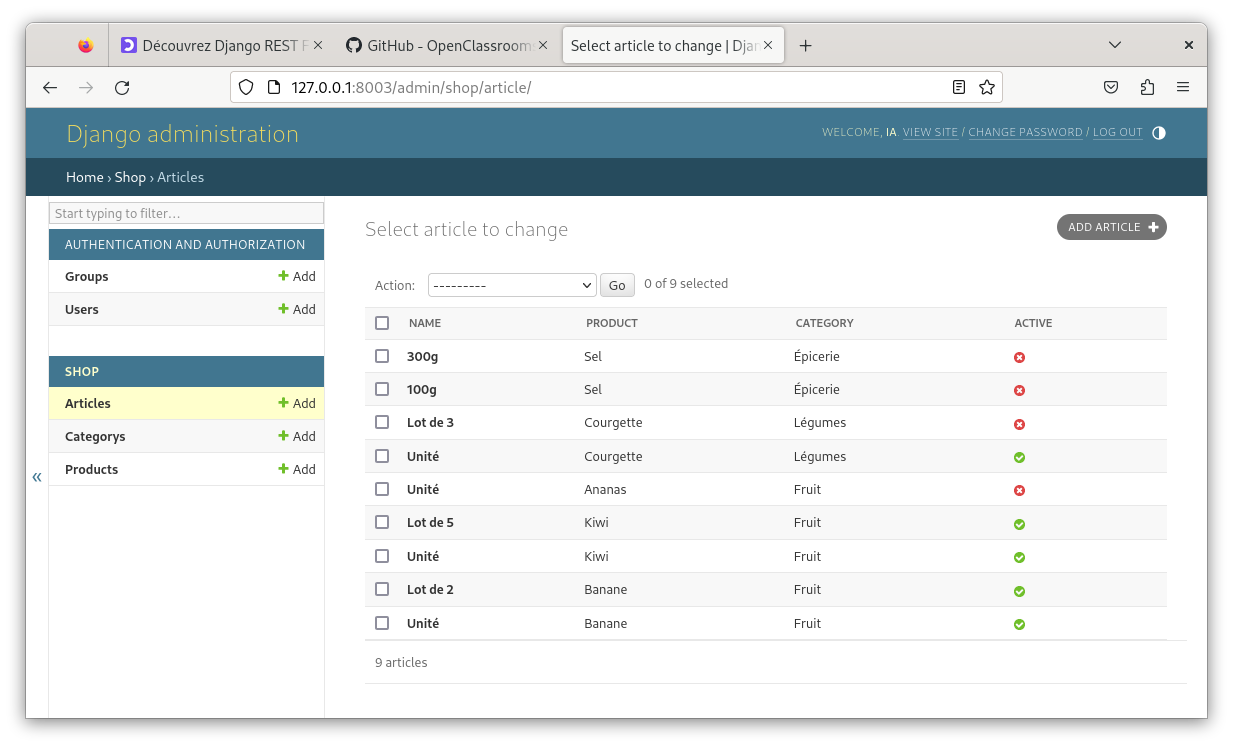
\includegraphics[width=10cm]{images/image04.png}
\end{center}

Allez dans le dossier :
\begin{minted}[
mathescape,
framesep=2mm,
baselinestretch=1.2,
%fontsize=\footnotesize,
bgcolor=LightGray,
%linenos
]{bash}
cd boutique
\end{minted}
Bien sûr adaptez {\color{monOrange}boutique} avec le nom que vous avez donné au projet.

Installez les dépendances :
\begin{minted}[
mathescape,
framesep=2mm,
baselinestretch=1.2,
%fontsize=\footnotesize,
bgcolor=LightGray,
%linenos
]{bash}
npm install
\end{minted}
Ouvrez {\color{monOrange}VS Code} et chargez le projet :
\begin{minted}[
mathescape,
framesep=2mm,
baselinestretch=1.2,
%fontsize=\footnotesize,
bgcolor=LightGray,
%linenos
]{bash}
code .
\end{minted}

\subsection{Inclusion d'une police}
Nous modifions {\color{monOrange}index.html} pour charger une police depuis {\color{monOrange}Google API} :
\begin{minted}[
mathescape,
framesep=2mm,
baselinestretch=1.2,
%fontsize=\footnotesize,
bgcolor=LightGray,
%linenos
]{html}
<!DOCTYPE html>
<html lang="fr">
  <head>
    <meta charset="UTF-8" />
    <link rel="icon" href="/favicon.ico" />
    <meta name="viewport" content="width=device-width, initial-scale=1.0" />
    <title>Vite App</title>
    <link rel="preconnect" href="https://fonts.googleapis.com" />
    <link rel="preconnect" href="https://fonts.gstatic.com" crossorigin />
    <link
      href="https://fonts.googleapis.com/css2?family=Roboto:wght@400;500;700&display=swap"
      rel="stylesheet"
    />
  </head>
  <body>
    <div id="app"></div>
    <script type="module" src="/src/main.ts"></script>
  </body>
</html>
\end{minted}

\subsection{Modification de {\color{monOrange}App.vue}}
Nous enlevons tout le code par défaut et ajoutons l'utilisation de {\color{monOrange}scss} :
\begin{minted}[
mathescape,
framesep=2mm,
baselinestretch=1.2,
%fontsize=\footnotesize,
bgcolor=LightGray,
%linenos
]{html}
<script setup lang="ts"></script>

<template>
  <h1>Bonjour le monde !</h1>
</template>

<style lang="scss">
@use './assets/base.scss' as *;
</style>
\end{minted}
\begin{center}
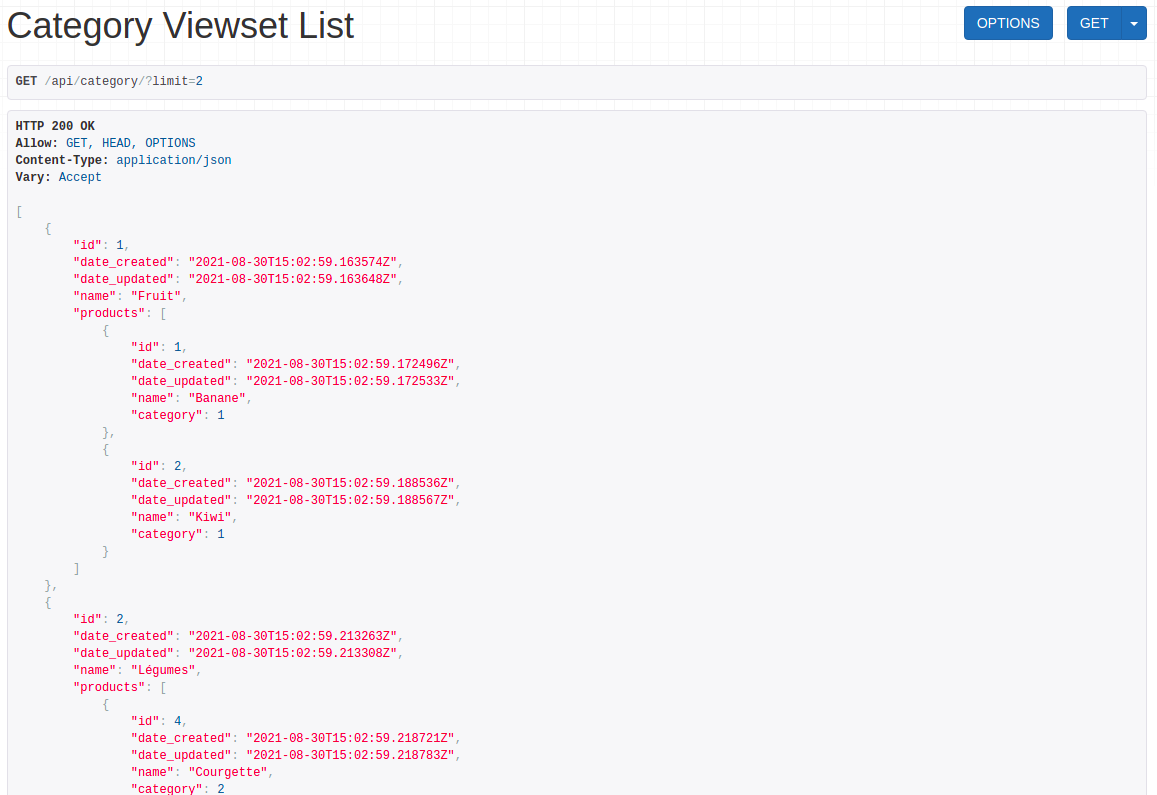
\includegraphics[width=10cm]{images/image14.png}
\end{center}
\subsection{Installation de {\color{monOrange}Sass}}
Installez Sass en dépendance de développement :
\begin{minted}[
mathescape,
framesep=2mm,
baselinestretch=1.2,
%fontsize=\footnotesize,
bgcolor=LightGray,
%linenos
]{bash}
npm i -D sass
\end{minted}

\subsection{Modification de {\color{monOrange}assets/base.css}}
Renommez le fichier {\color{monOrange}base.css} en {\color{monOrange}base.scss} car nous utilisons {\color{monOrange}Sass} et mettez pour le moment :
\begin{minted}[
mathescape,
framesep=2mm,
baselinestretch=1.2,
%fontsize=\footnotesize,
bgcolor=LightGray,
%linenos
]{scss}
:root {
  --font-family: 'Roboto', sans-serif;
}

body {
  font-family: var(--font-family);
}
\end{minted}

\subsection{Installation de l'extension pour navigateur {\color{monOrange}Vue}}
Installez l'extension Chrome pour Vue.js ou l'extension Firefox suivant votre navigateur.

Le nom de l'extension est Vue.js devtools.

\subsection{Extensions pour {\color{monOrange}Visual Studio Code}}
Vérifiez dans extensions sur VS Code que vous avez bien installé Volar et Volar TypeScript.

Vérifiez que l'extension {\color{monOrange}@builtin typescript} est bien désactivée pour le {\color{monOrange}workspace}.

%Exemple exécutable de la vidéo
%Vous pouvez directement utiliser ce code exécutable. N'hésitez pas à l'ouvrir dans un nouvel onglet pour le modifier ou mieux voir :

%%%%%%%%%%%%%%%%%%%%%%%%%%%%%%%%%%%%%%%%%%%%%%%%%%%%%%%%%%

\section{Mise en place du style}
\subsection{Modification deassets/base.scss}
Utilisez le style de base suivant :
\begin{minted}[
mathescape,
framesep=2mm,
baselinestretch=1.2,
fontsize=\footnotesize,
bgcolor=LightGray,
%linenos
]{scss}
:root {
  --primary-1: #3498db;
  --primary-2: #2980b9;
  --danger-1: #e74c3c;
  --danger-2: #c0392b;
  --success-1: #2ecc71;
  --success-2: #27ae60;
  --gray-1: #f6f6f6;
  --gray-2: #ddd;
  --gray-3: #34495e;
  --text-color: #444;
  --text-primary-color: #ffffff;

  --border: 1px solid var(--gray-2);
  --border-radius: 4px;

  --font-family: 'Roboto', sans-serif;
}
// reset
* {
  box-sizing: border-box;
}
h1,h2,h3,h4 {
  margin: 0;
}
ul {
  list-style: none;
  padding: 0;
}
img {
  max-width: 100%;
}
a {
  color: var(--text-color);
  text-decoration: none;
}
body {
  min-height: 100vh;
  padding: 0;
  margin: 0;
  font-family: var(--font-family);
  color: var(--text-color);
  background-color: var(--gray-1);
}
// flex
.d-flex {  display: flex; }
.flex-row {  flex-direction: row; }
.flex-column { flex-direction: column; }
.justify-content-center {  justify-content: center; }
.align-items-center {  align-items: center; }
.flex-fill {  flex: 1 1 auto; }
// padding
.p-10 {  padding: 10px; }
.p-20 {  padding: 20px; }
.p-30 {  padding: 30px; }
// margin
.m-10 {  margin: 10px; }
.m-20 {  margin: 20px; }
.m-30 {  margin: 30px; }
\end{minted}

Si vous ne maîtrisez pas certaines propriétés, n'hésitez pas à revoir les chapitres correspondants dans la formation HTML \& CSS.

\subsection{Création du fichier assets/debug.scss}
Créez les classes pour le débug plus facile du CSS :
\begin{minted}[
mathescape,
framesep=2mm,
baselinestretch=1.2,
fontsize=\footnotesize,
bgcolor=LightGray,
%linenos
]{css}
.b1 {  background-color: red; }
.b2 {  background-color: blue; }
.b3 {  background-color: yellow; }
.b4 {  background-color: green; }
.b5 {  background-color: purple; }
\end{minted}

Photocopieuse
\subsection{Modification de App.vue}
N'oubliez pas de modifier App.vue pour l'importer :
\begin{minted}[
mathescape,
framesep=2mm,
baselinestretch=1.2,
%fontsize=\footnotesize,
bgcolor=LightGray,
%linenos
]{html}
<script setup lang="ts"></script>

<template>
  <h1>Bonjour le monde !</h1>
</template>

<style lang="scss">
@use './assets/base.scss' as *;
@use './assets/debug.scss' as *;
</style>
\end{minted}

%Exemple exécutable de la vidéo
%Vous pouvez directement utiliser ce code exécutable. N'hésitez pas à l'ouvrir dans un nouvel onglet pour le modifier ou mieux voir :

%%%%%%%%%%%%%%%%%%%%%%%%%%%%%%%%%%%%%%%%%%%%%%%%%%%%%%%%%%%%%%

\section{Mise en page globale}
\subsection{Création de l'architecture}
Créez un dossier {\color{monOrange}components} dans le dossier {\color{monOrange}src}.

Dans ce dossier, créez les fichiers {\color{monOrange}Footer.vue, Header.vue, Shop.vue} et {\color{monOrange}Cart.vue}.

\subsubsection{Composant {\color{monOrange}Footer.vue}}
Mettez dans le composant :
\begin{minted}[
mathescape,
framesep=2mm,
baselinestretch=1.2,
fontsize=\footnotesize,
bgcolor=LightGray,
%linenos
]{html}
<script setup lang="ts"></script>

<template>
  <footer>
    <h1>Footer</h1>
  </footer>
</template>

<style lang="scss" scoped></style>
\end{minted}

\subsubsection{Composant {\color{monOrange}Header.vue}}
Mettez dans le composant :
\begin{minted}[
mathescape,
framesep=2mm,
baselinestretch=1.2,
fontsize=\footnotesize,
bgcolor=LightGray,
%linenos
]{html}
<script setup lang="ts"></script>

<template>
  <header>
    <h1>Header</h1>
  </header>
</template>

<style lang="scss" scoped></style>
\end{minted}

\subsubsection{Composant {\color{monOrange}Shop.vue}}
Mettez dans le composant :
\begin{minted}[
mathescape,
framesep=2mm,
baselinestretch=1.2,
fontsize=\footnotesize,
bgcolor=LightGray,
%linenos
]{html}
<script setup lang="ts"></script>

<template>
  <div>
    <h1>Shop</h1>
  </div>
</template>

<style lang="scss" scoped></style>
\end{minted}

\subsubsection{Composant {\color{monOrange}Cart.vue}}
Mettez dans le composant :
\begin{minted}[
mathescape,
framesep=2mm,
baselinestretch=1.2,
fontsize=\footnotesize,
bgcolor=LightGray,
%linenos
]{html}
<script setup lang="ts"></script>

<template>
  <div>
    <h1>Cart</h1>
  </div>
</template>

<style lang="scss" scoped></style>
\end{minted}

Notez que nous utilisons {\color{monOrange}scoped} pour limiter la portée des styles déclarés dans ces composants.

\subsubsection{Modification de {\color{monOrange}App.vue}}
Modifications de notre composant racine pour importer et utiliser les composants que nous avons créés :
\begin{minted}[
mathescape,
framesep=2mm,
baselinestretch=1.2,
fontsize=\footnotesize,
bgcolor=LightGray,
%linenos
]{html}
<script setup lang="ts">
import TheHeader from './components/Header.vue';
import TheFooter from './components/Footer.vue';
import Shop from './components/Shop.vue';
import Cart from './components/Cart.vue';
</script>

<template>
  <div class="app-container">
    <TheHeader class="header b1" />
    <Shop class="shop b2" />
    <Cart class="cart b3" />
    <TheFooter class="footer b4" />
  </div>
</template>

<style lang="scss">
@use './assets/base.scss' as *;
@use './assets/debug.scss' as *;

.app-container {
  min-height: 100vh;
  display: grid;
  grid-template-areas: 'header header' 'shop cart' 'footer footer';
  grid-template-columns: 75% 25%;
  grid-template-rows: 48px auto 48px;
}
.header {  grid-area: header; }
.shop {  grid-area: shop; }
.cart {  grid-area: cart; }
.footer {  grid-area: footer; }
</style>
\end{minted}

{\em Nous utilisons une grille {\color{monOrange}CSS}, n'hésitez pas à revoir le chapitre sur les grilles dans la formation {\color{monOrange}CSS}}.

\begin{center}
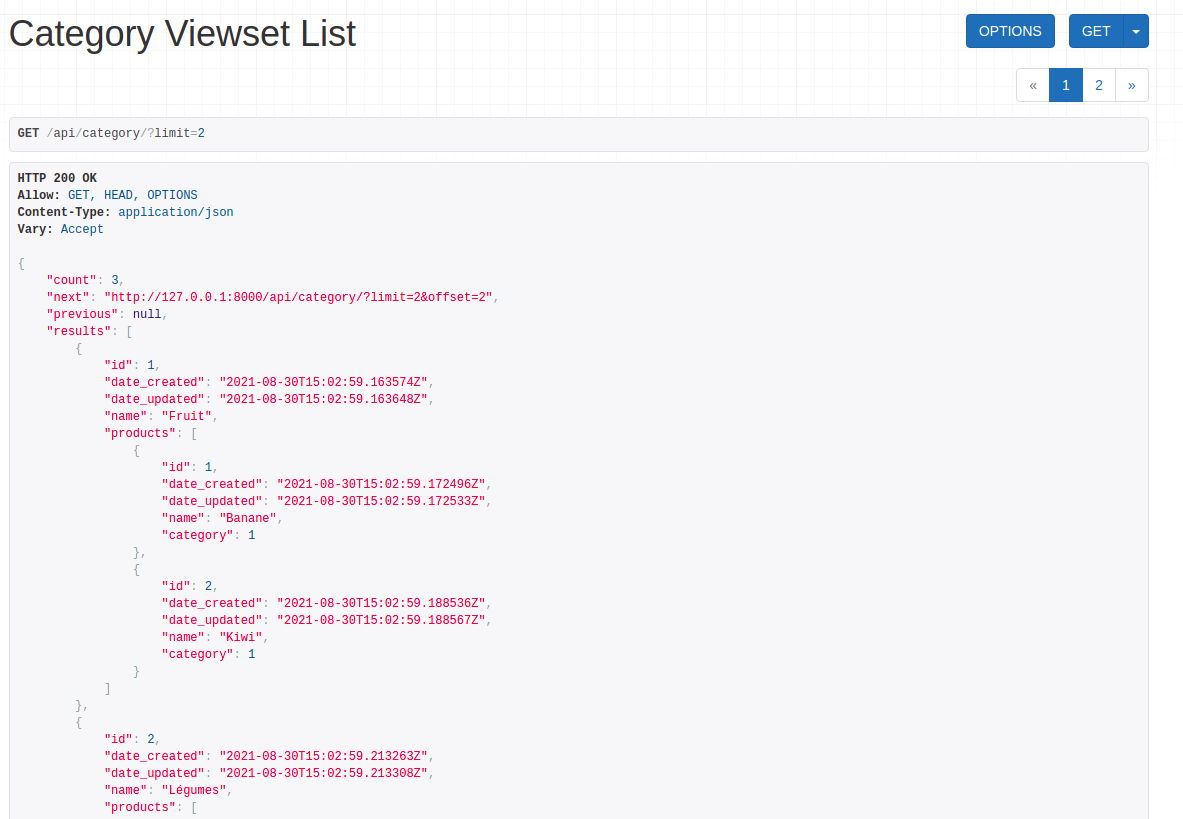
\includegraphics[width=15cm]{images/image15.png}
\end{center}
%Exemple exécutable de la vidéo
%Vous pouvez directement utiliser ce code exécutable. N'hésitez pas à l'ouvrir dans un nouvel onglet pour le modifier ou mieux voir :

%%%%%%%%%%%%%%%%%%%%%%%%%%%%%%%%%%%%%%%%%%%%%%%%%%%%%%%%%%%%

\section{Mise en page boutique et panier}
\subsection{Architecture}
Dans le dossier components créez un dossier Cart et un dossier Shop.

Déplacez le composant Cart.vue dans Cart et Shop.vue dans Shop.

Commencez à jour les chemins d'imports dans App.vue :
\begin{minted}[
mathescape,
framesep=2mm,
baselinestretch=1.2,
fontsize=\footnotesize,
bgcolor=LightGray,
%linenos
]{html}
<script setup lang="ts">
import TheHeader from './components/Header.vue';
import TheFooter from './components/Footer.vue';
import Shop from './components/Shop/Shop.vue';
import Cart from './components/Cart/Cart.vue';
</script>
\end{minted}

Dans le dossier Cart, créez les composants CartProductList.vue et CartProduct.vue.

Même choisi dans le dossier Shop, créé deux composants ShopProductList.vue et ShopProduct.vue.

\subsection{Modification de {\color{monOrange}Shop.vue}}
Nous allons importer et utiliser les nouveaux composants relatifs à la liste des produits :
\begin{minted}[
mathescape,
framesep=2mm,
baselinestretch=1.2,
fontsize=\footnotesize,
bgcolor=LightGray,
%linenos
]{html}
<script setup lang="ts">
import ShopProductList from './ShopProductList.vue';
</script>

<template>
  <div>
    <ShopProductList />
  </div>
</template>

<style lang="scss" scoped></style>
\end{minted}
Dans ce composant nous plaçons le composant qui va être responsable de gérer la liste des produits.

\subsection{Modification de ShopProductList.vue}
Dans ce composant nous allons utiliser plusieurs instances de notre composant ShopProduct et les disposer en utilisant une grille CSS :
\begin{minted}[
mathescape,
framesep=2mm,
baselinestretch=1.2,
fontsize=\footnotesize,
bgcolor=LightGray,
%linenos
]{html}
<script setup lang="ts">
import ShopProduct from './ShopProduct.vue';
</script>

<template>
  <div class="grid p-20">
    <ShopProduct />
    <ShopProduct />
    <ShopProduct />
    <ShopProduct />
    <ShopProduct />
    <ShopProduct />
    <ShopProduct />
    <ShopProduct />
    <ShopProduct />
  </div>
</template>

<style lang="scss" scoped>
.grid {
  display: grid;
  grid-template-columns: 1fr 1fr 1fr 1fr;
  grid-auto-rows: 300px;
  gap: 20px;
}
</style>
\end{minted}

\subsection{Modification de ShopProduct.vue}
Dans ce composant nous affichons juste un titre pour le moment :
\begin{minted}[
mathescape,
framesep=2mm,
baselinestretch=1.2,
fontsize=\footnotesize,
bgcolor=LightGray,
%linenos
]{html}
<script setup lang="ts"></script>

<template>
  <div class="b5">
    <h1>Shop Product</h1>
  </div>
</template>

<style lang="scss" scoped></style>
\end{minted}

\subsection{Modification de Cart.vue}
Dans ce composant nous utilisons le composant CartProductList responsable de gérer l'affichage des produits du panier :
\begin{minted}[
mathescape,
framesep=2mm,
baselinestretch=1.2,
fontsize=\footnotesize,
bgcolor=LightGray,
%linenos
]{html}
<script setup lang="ts">
import CartProductList from './CartProductList.vue';
</script>

<template>
  <div class="p-20">
    <h2 class="mb-10">Panier</h2>
    <CartProductList />
  </div>
</template>

<style lang="scss" scoped></style>
\end{minted}

N'oubliez pas de modifier assets/base.scss pour ajouter la classe mb-10 :
\begin{minted}[
mathescape,
framesep=2mm,
baselinestretch=1.2,
fontsize=\footnotesize,
bgcolor=LightGray,
%linenos
]{html}
.mb-10 {
  margin-bottom: 10px;
}
\end{minted}

\subsection{Modification de CartProductList.vue}
Dans ce composant nous allons utiliser plusieurs instances du composant CartProduct qui sont les produits dans le panier.

Nous utilisons des boîtes flexibles pour positionner les produits.
\begin{minted}[
mathescape,
framesep=2mm,
baselinestretch=1.2,
fontsize=\footnotesize,
bgcolor=LightGray,
%linenos
]{html}
<script setup lang="ts">
import CartProduct from './CartProduct.vue';
</script>

<template>
  <div class="d-flex flex-column">
    <CartProduct />
    <CartProduct />
    <CartProduct />
    <CartProduct />
    <CartProduct />
    <CartProduct />
  </div>
</template>

<style lang="scss" scoped></style>
\end{minted}

\subsection{Modification de CartProduct.vue}
Dans ce composant nous affichons pour le moment simplement un titre :
\begin{minted}[
mathescape,
framesep=2mm,
baselinestretch=1.2,
fontsize=\footnotesize,
bgcolor=LightGray,
%linenos
]{html}
<script setup lang="ts"></script>

<template>
  <div class="mb-10 b5">
    <h1>Product</h1>
  </div>
</template>

<style lang="scss" scoped></style>
\end{minted}
\begin{center}
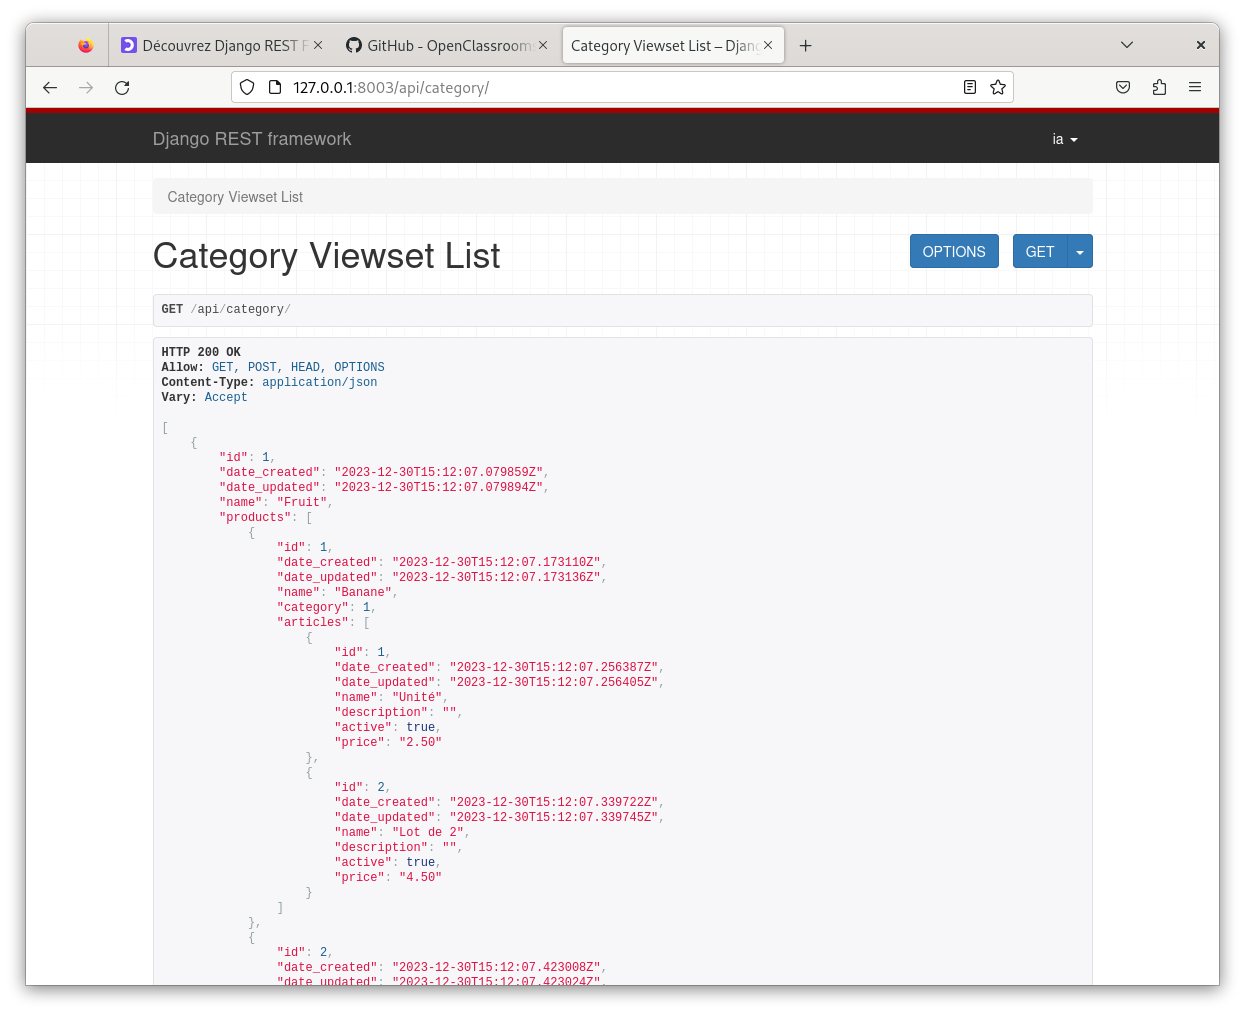
\includegraphics[width=12cm]{images/image16.png}
\end{center}
%Exemple exécutable de la vidéo
%Vous pouvez directement utiliser ce code exécutable. N'hésitez pas à l'ouvrir dans un nouvel onglet pour le modifier ou mieux voir :

%%%%%%%%%%%%%%%%%%%%%%%%%%%%%%%%%%%%%%%%%%%%%%%%%%%%%%%%%%%%%%

\section{Mise en page du header et du footer}
\subsection{Modification deassets/base.scss}
Ajoutez les classes utilitaires dont nous aurons besoin :
\begin{minted}[
mathescape,
framesep=2mm,
baselinestretch=1.2,
fontsize=\footnotesize,
bgcolor=LightGray,
%linenos
]{css}
.px-20 {
  padding-left: 20px;
  padding-right: 20px;
}
.p-30 { padding: 30px; }
// margin
.m-10 { margin: 10px; }
.mb-10 { margin-bottom: 10px; }
.mr-10 { margin-right: 10px; }
.mr-20 {  margin-right: 20px; }
\end{minted}

\subsection{Modification de Header.vue}
Nous mettons en place notre header :
\begin{minted}[
mathescape,
framesep=2mm,
baselinestretch=1.2,
fontsize=\footnotesize,
bgcolor=LightGray,
%linenos
]{html}
<script setup lang="ts"></script>

<template>
  <header class="px-20 d-flex flex-row align-items-center">
    <a href="#" class="d-flex flex-row align-items-center mr-20">
      <img src="../assets/logo.svg" />
      <span class="logo">Dyma</span>
    </a>
    <ul class="d-flex flex-row flex-fill">
      <li class="mr-10">
        <a href="#">Boutique</a>
      </li>
      <li>
        <a href="#">Admin</a>
      </li>
    </ul>
    <ul class="d-flex flex-row">
      <li class="mr-10">
        <a href="#">Inscription</a>
      </li>
      <li>
        <a href="#">Connexion</a>
      </li>
    </ul>
  </header>
</template>

<style lang="scss" scoped>
header {
  background-color: var(--primary-1);
  a {
    color: var(--text-primary-color);
    img {
      width: 20px;
      margin-right: 5px;
    }
    .logo {
      font-weight: 700;
      font-size: 20px;
    }
  }
}
</style>
\end{minted}

\subsection{Modification de Footer.vue}
Nous mettons en place notre footer :
\begin{minted}[
mathescape,
framesep=2mm,
baselinestretch=1.2,
fontsize=\footnotesize,
bgcolor=LightGray,
%linenos
]{html}
<script setup lang="ts"></script>

<template>
  <footer class="d-flex flex-row justify-content-center align-items-center">
    <p>Copyright © 2014-2022 Dyma</p>
  </footer>
</template>

<style lang="scss" scoped>
footer {
  background-color: var(--gray-3);
  color: var(--text-primary-color);
}
</style>
\end{minted}
\begin{center}
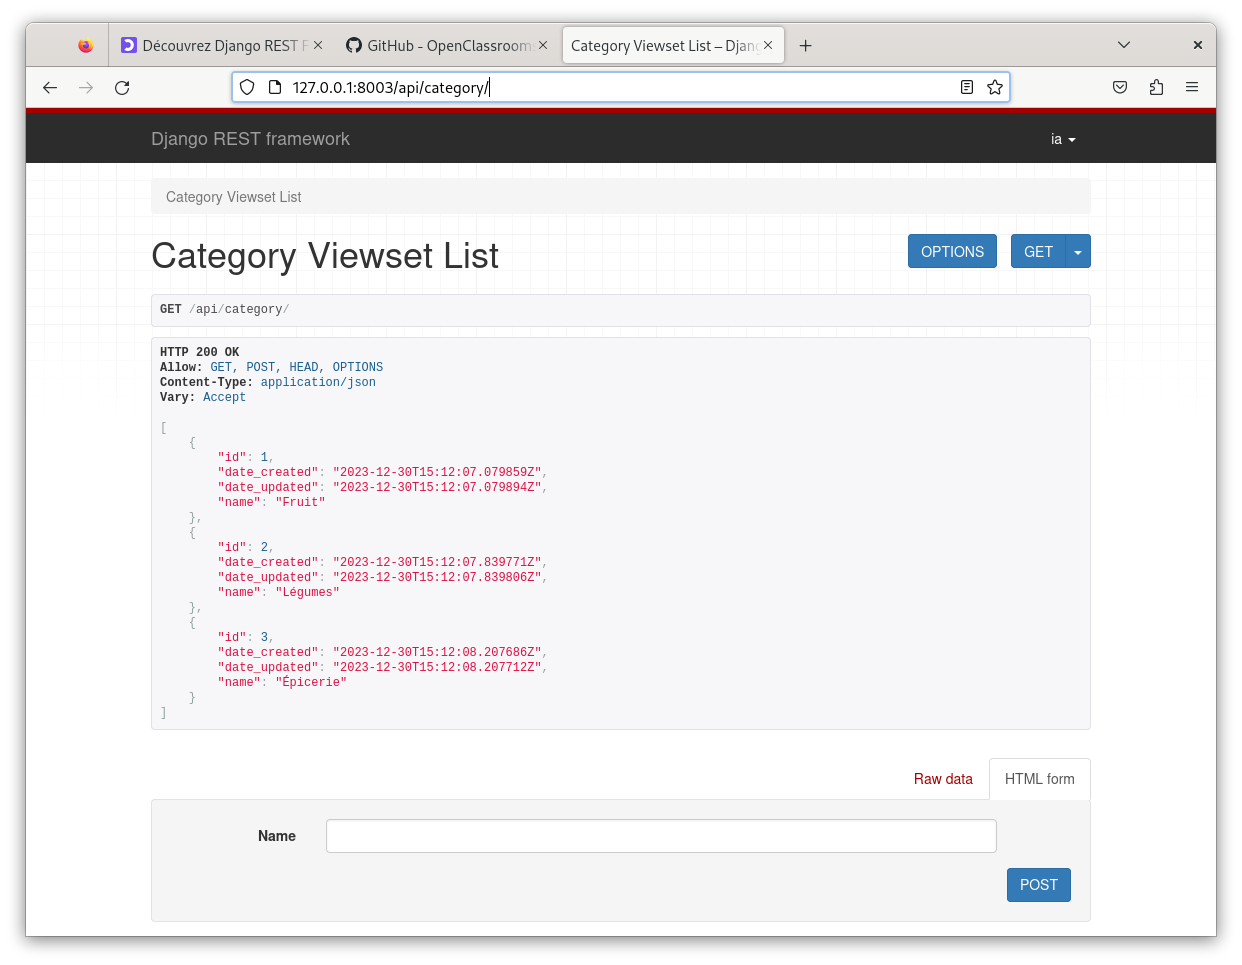
\includegraphics[width=15cm]{images/image17.png}
\end{center}
%Exemple exécutable de la vidéo
%Vous pouvez directement utiliser ce code exécutable. N'hésitez pas à l'ouvrir dans un nouvel onglet pour le modifier ou mieux voir :

%%%%%%%%%%%%%%%%%%%%%%%%%%%%%%%%%%%%%%%%%%%%%%%%%%%%%%%%%%%

\section{Mise en page de la partie Shop}
\subsection{Modification de {\color{monOrange}ShopProduct.vue}}
Nous mettons pour le moment les détails du produit en dur :
\begin{minted}[
mathescape,
framesep=2mm,
baselinestretch=1.2,
fontsize=\footnotesize,
bgcolor=LightGray,
%linenos
]{html}
<script setup lang="ts"></script>

<template>
  <div class="product d-flex flex-column">
    <div class="product-image"></div>
    <div class="p-10 d-flex flex-column">
      <h4>Macbook Pro</h4>
      <p>Performances exceptionnelles avec la puce M1 Pro ou M1</p>
      <div class="d-flex flex-row align-items-center">
        <strong class="flex-fill">Prix : 1500€</strong>
        <button class="btn btn-primary">Ajouter au panier</button>
      </div>
    </div>
  </div>
</template>

<style lang="scss" scoped>
.product {
  background-color: #ffffff;
  border: var(--border);
  border-radius: var(--border-radius);
  &-image {
    border-top-right-radius: var(--border-radius);
    border-top-left-radius: var(--border-radius);
    background-image: url('https://media.ldlc.com/r1600/ld/products/00/05/82/01/LD0005820198_1.jpg');
    background-size: cover;
    background-position: center;
    height: 250px;
  }
}
</style>
\end{minted}

Photocopieuse
\subsection{Classes pour les boutons}
Modifiez {\color{monOrange}assets/base.scss} pour ajouter les classes pour nos boutons :
\begin{minted}[
mathescape,
framesep=2mm,
baselinestretch=1.2,
fontsize=\footnotesize,
bgcolor=LightGray,
%linenos
]{scss}
// buttons

.btn {
  padding: 8px 15px;
  border: 0;
  border-radius: var(--border-radius);
  cursor: pointer;
  font-weight: 500;
  transition: background-color 0.2s;
}

.btn-primary {
  background-color: var(--primary-1);
  color: var(--text-primary-color);
  &:hover {
    background-color: var(--primary-2);
  }
}

.btn-danger {
  background-color: var(--danger-1);
  color: var(--text-primary-color);
  &:hover {
    background-color: var(--danger-2);
  }
}
\end{minted}
\begin{center}
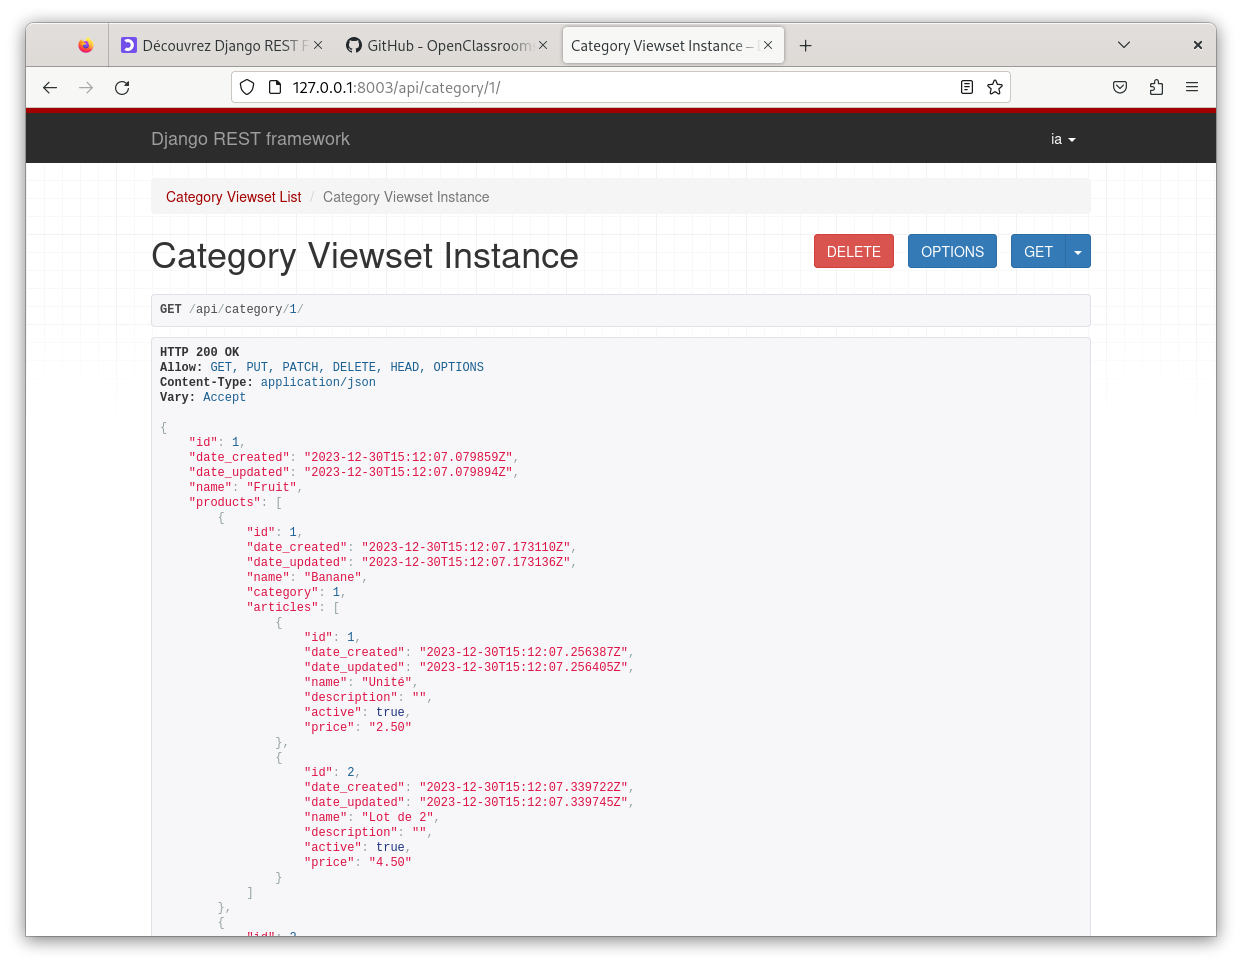
\includegraphics[width=15cm]{images/image18.png}
\end{center}
%Exemple exécutable de la vidéo
%Vous pouvez directement utiliser ce code exécutable. N'hésitez pas à l'ouvrir dans un nouvel onglet pour le modifier ou mieux voir :

%%%%%%%%%%%%%%%%%%%%%%%%%%%%%%%%%%%%%%%%%%%%%%%%%%%%%%%%%%%%%%%%

\section{Mise en place du panier}
\subsection{Modification de {\color{monOrange}CartProduct.vue}}
Nous mettons en place en dur le produit du panier pour terminer la mise en page :
\begin{minted}[
mathescape,
framesep=2mm,
baselinestretch=1.2,
fontsize=\footnotesize,
bgcolor=LightGray,
%linenos
]{html}
<script setup lang="ts"></script>

<template>
  <div class="mb-10 p-10 d-flex flex-row align-items-center product">
    <strong class="flex-fill mr-10">Macbook Pro</strong>
    <span class="mr-10">Prix : 1500€</span>
    <button class="btn btn-danger">Supprimer</button>
  </div>
</template>

<style lang="scss" scoped>
.product {
  border: var(--border);
  border-radius: var(--border-radius);
  background-color: var(--gray-1);
}
</style>
\end{minted}

\subsection{Modification de {\color{monOrange}App.vue}}
Nous modifions légèrement la classe {\color{monOrange}cart} :
\begin{minted}[
mathescape,
framesep=2mm,
baselinestretch=1.2,
fontsize=\footnotesize,
bgcolor=LightGray,
%linenos
]{html}
<style lang="scss">
@use './assets/base.scss' as *;
@use './assets/debug.scss' as *;

.app-container {
  min-height: 100vh;
  display: grid;
  grid-template-areas: 'header header' 'shop cart' 'footer footer';
  grid-template-columns: 75% 25%;
  grid-template-rows: 48px auto 48px;
}
.header {
  grid-area: header;
}
.shop {
  grid-area: shop;
}
.cart {
  grid-area: cart;
  border-left: var(--border);
  background-color: white;
}
.footer {
  grid-area: footer;
}
</style> 
\end{minted}

\begin{center}
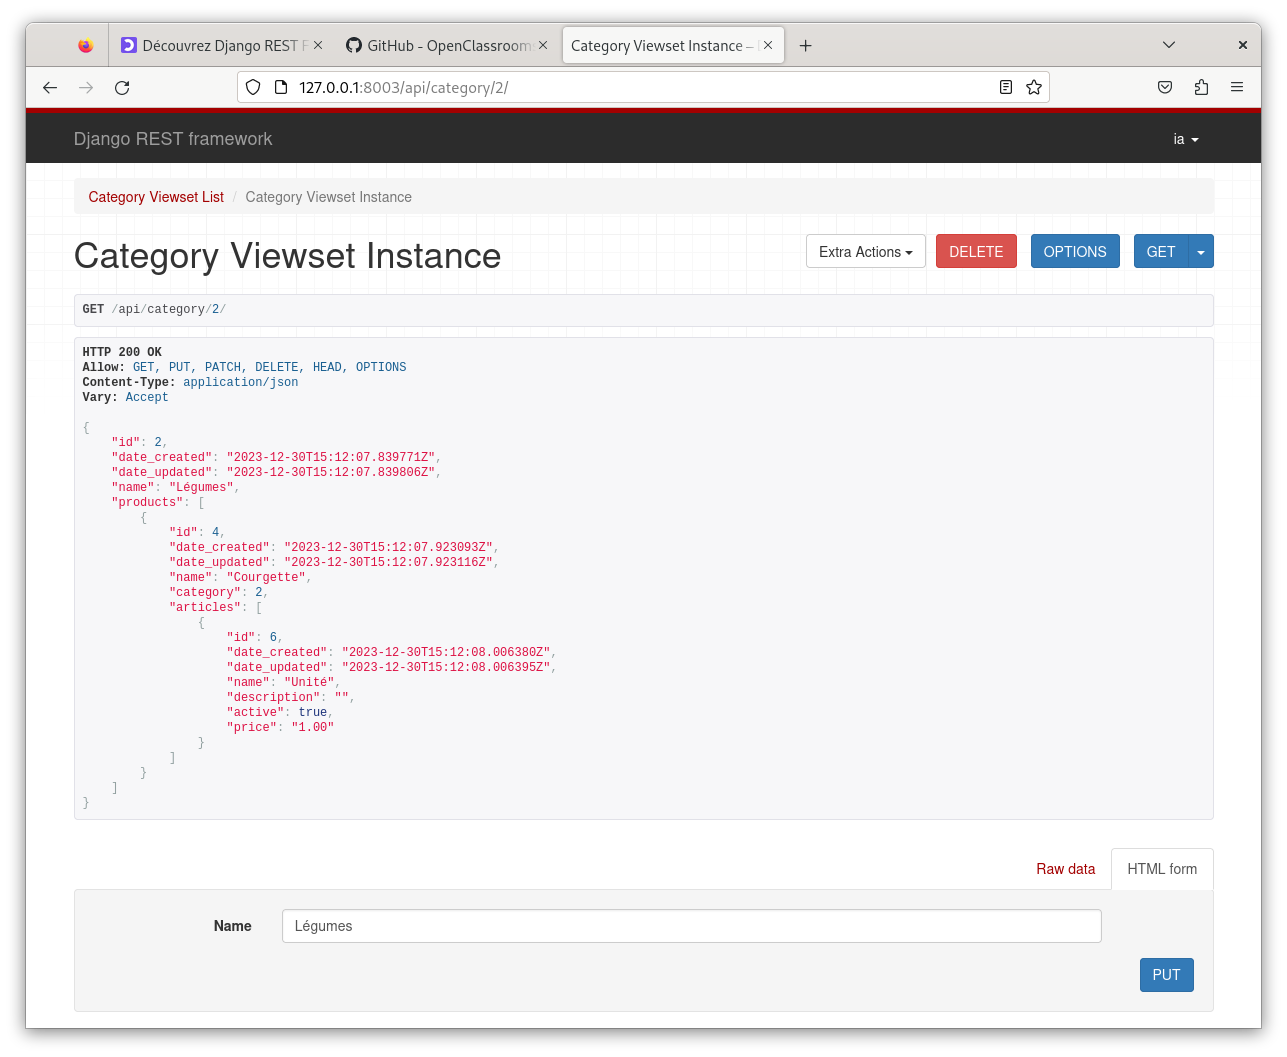
\includegraphics[width=15cm]{images/image19.png}
\end{center}
%Exemple exécutable de la vidéo
%Vous pouvez directement utiliser ce code exécutable. N'hésitez pas à l'ouvrir dans un nouvel onglet pour le modifier ou mieux voir :
%%%%%%%%%%%%%%%%%%%%%%%%%%%%%%%%%%%%%%%%%%%%%%%%%%%%%%
\section{Utilisation des props pour les produits}
\subsection{Création des interfaces}
Créez un dossier interfaces dans src.

Créer dans ce dossier un fichier Product.interface.ts :
\begin{minted}[
mathescape,
framesep=2mm,
baselinestretch=1.2,
fontsize=\footnotesize,
bgcolor=LightGray,
%linenos
]{javascript}
export interface ProductInterface {
    title: string;
    image: string;
    price: number;
    description: string;
}
\end{minted}
\subsection{Données en dur}
En attendant d'avancer plus dans le projet et d'utiliser des requêtes HTTP pour récupérer les produits, nous allons mettre les données en dur.

Pour ce faire, créez un dossier data dans src.

Dans ce dossier, créez un fichier product.ts :
\begin{minted}[
mathescape,
framesep=2mm,
baselinestretch=1.2,
fontsize=\footnotesize,
bgcolor=LightGray,
%linenos
]{javascript}
export default [
  {
    id: 1,
    image: 'src/assets/images/macbookpro.PNG',
    title: 'Macbook Pro',
    description:
      'Lorem ipsum dolor sit amet consectetur adipisicing edolor tempore ipsam cum ipsum reiciendis',
    price: 1500,
  },
  {
    id: 2,
    image: 'src/assets/images/levono.PNG',
    title: 'Levono Pro',
    description:
      'Lorem ipsum dolor sit amet consectetur adipisicing edolor tempore ipsam cum ipsum reiciendis',
    price: 2300,
  },
  {
    id: 3,
    image: 'src/assets/images/rider.PNG',
    title: 'Rider',
    description:
      'Lorem ipsum dolor sit amet consectetur adipisicing edolor tempore ipsam cum ipsum reiciendis',
    price: 1200,
  },
  {
    id: 4,
    image: 'src/assets/images/ldlc.PNG',
    title: 'LDLC benolo',
    description:
      'Lorem ipsum dolor sit amet consectetur adipisicing edolor tempore ipsam cum ipsum reiciendis',
    price: 4500,
  },
  {
    id: 5,
    image: 'src/assets/images/asus.PNG',
    title: 'Asus gamer',
    description:
      'Lorem ipsum dolor sit amet consectetur adipisicing edolor tempore ipsam cum ipsum reiciendis',
    price: 3755,
  },
  {
    id: 6,
    image: 'src/assets/images/rog.PNG',
    title: 'Rog desktop',
    description:
      'Lorem ipsum dolor sit amet consectetur adipisicing edolor tempore ipsam cum ipsum reiciendis',
    price: 2452,
  },
  {
    id: 7,
    image: 'src/assets/images/msi.PNG',
    title: 'MSI play',
    description:
      'Lorem ipsum dolor sit amet consectetur adipisicing edolor tempore ipsam cum ipsum reiciendis',
    price: 1478,
  },
  {
    id: 8,
    image: 'src/assets/images/pad.PNG',
    title: 'Think pad',
    description:
      'Lorem ipsum dolor sit amet consectetur adipisicing edolor tempore ipsam cum ipsum reiciendis',
    price: 899,
  },
];
\end{minted}
\subsection{Modification de App.vue}
Dans le composant racine, nous allons importer les données et les typer dans une propriété réactive.

Nous allons ensuite les passer à notre composant enfant Shop en utilisant une liaison de données avec v-bind.
\begin{minted}[
mathescape,
framesep=2mm,
baselinestretch=1.2,
fontsize=\footnotesize,
bgcolor=LightGray,
%linenos
]{html}
<script setup lang="ts">
import TheHeader from './components/Header.vue';
import TheFooter from './components/Footer.vue';
import Shop from './components/Shop/Shop.vue';
import Cart from './components/Cart/Cart.vue';
import data from './data/product';

import { reactive } from 'vue';
import type { ProductInterface } from './interfaces';
const products = reactive<ProductInterface[]>(data);
</script>

<template>
  <div class="app-container">
    <TheHeader class="header" />
    <Shop :products="products" class="shop" />
    <Cart class="cart" />
    <TheFooter class="footer" />
  </div>
</template>

<style lang="scss">
@use './assets/base.scss' as *;
@use './assets/debug.scss' as *;

.app-container {
  min-height: 100vh;
  display: grid;
  grid-template-areas: 'header header' 'shop cart' 'footer footer';
  grid-template-columns: 75% 25%;
  grid-template-rows: 48px auto 48px;
}
.header {
  grid-area: header;
}
.shop {
  grid-area: shop;
}
.cart {
  grid-area: cart;
  border-left: var(--border);
  background-color: white;
}
.footer {
  grid-area: footer;
}
</style>
\end{minted}
{\tt reactive<ProductInterface[]>(data)} : nous passons en type générique un tableau de produits qui doivent respecter l'interface {\color{monOrange}ProductInterface}. Nous initialisons la propriété réactive avec nos données contenues dans {\color{monOrange}data}.

\subsection{Modification de {\color{monOrange}Shop.vue}}
Dans le composant {\color{monOrange}Shop.vue}, nous définissons la {\color{monOrange}prop} reçue depuis le composant parent grâce à {\color{monOrange}defineProps}, à savoir la liste de tous les produits.

Nous typons la {\color{monOrange}props} en passant le type générique {\tt  \{ products: ProductInterface[] \}} : cela signifie que nous recevons un objet contenant une propriété {\color{monOrange}products} qui a pour valeur un tableau contenant des {\color{monOrange}ProductInterface}.

Nous repassons ensuite la {\color{monOrange}prop} reçue plus bas dans l'arbre :
\begin{minted}[
mathescape,
framesep=2mm,
baselinestretch=1.2,
fontsize=\footnotesize,
bgcolor=LightGray,
%linenos
]{html}
<script setup lang="ts">
import type { ProductInterface } from '@/interfaces';
import ShopProductList from './ShopProductList.vue';

defineProps<{
  products: ProductInterface[];
}>();
</script>

<template>
  <div>
    <ShopProductList :products="products" />
  </div>
</template>

<style lang="scss" scoped></style>
\end{minted}
\subsection{Modification de {\color{monOrange}ShopProductList.vue}}
Dans le composant {\color{monOrange}ShopProductList}, nous récupérons également la {\color{monOrange}prop} que nous typons comme dans le composant parent {\color{monOrange}Shop}.

Cette fois, nous utilisons la directive {\color{monOrange}v-for} pour boucler sur les produits et nous utilisons une liaison de propriété pour passer le produit à chaque instance du composant {\color{monOrange}ShopProduct}.
\begin{minted}[
mathescape,
framesep=2mm,
baselinestretch=1.2,
fontsize=\footnotesize,
bgcolor=LightGray,
%linenos
]{html}
<script setup lang="ts">
import type { ProductInterface } from '@/interfaces';
import ShopProduct from './ShopProduct.vue';
defineProps<{
  products: ProductInterface[];
}>();
</script>

<template>
  <div class="grid p-20">
    <ShopProduct v-for="product of products" :product="product" />
  </div>
</template>

<style lang="scss" scoped>
.grid {
  display: grid;
  grid-template-columns: 1fr 1fr 1fr 1fr;
  grid-auto-rows: 400px;
  gap: 20px;
}
</style>
\end{minted}
\subsection{Modification de {\color{monOrange}ShopProduct.vue}}
Dans le composant {\color{monOrange}ShopProduct}, nous récupérons le produit en {\color{monOrange}props} et nous utilisons la notation raccourcie de la directive {\color{monOrange}v-text} pour afficher les différentes propriétés du produit.
\begin{minted}[
mathescape,
framesep=2mm,
baselinestretch=1.2,
fontsize=\footnotesize,
bgcolor=LightGray,
%linenos
]{scss}
<script setup lang="ts">
import type { ProductInterface } from '@/interfaces';
defineProps<{
  product: ProductInterface;
}>();
</script>

<template>
  <div class="product d-flex flex-column">
    <div
      class="product-image"
      :style="{ backgroundImage: `url(${product.image})` }"
    ></div>
    <div class="p-10 d-flex flex-column">
      <h4>{{ product.title }}</h4>
      <p>{{ product.description }}</p>
      <div class="d-flex flex-row align-items-center">
        <strong class="flex-fill">Prix : {{ product.price }}€</strong>
        <button class="btn btn-primary">Ajouter au panier</button>
      </div>
    </div>
  </div>
</template>

<style lang="scss" scoped>
.product {
  background-color: #ffffff;
  border: var(--border);
  border-radius: var(--border-radius);
  &-image {
    border-top-right-radius: var(--border-radius);
    border-top-left-radius: var(--border-radius);
    background-size: cover;
    background-position: center;
    height: 250px;
  }
}
</style>
\end{minted} 
\begin{center}
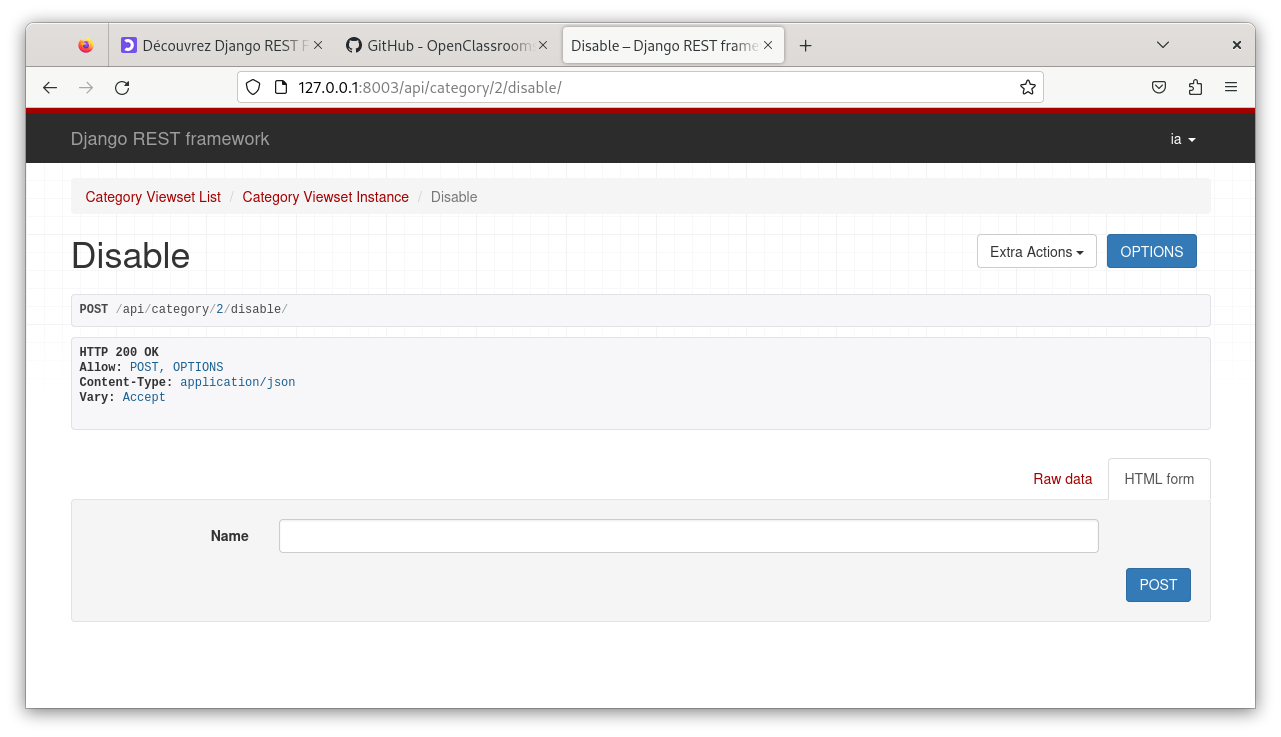
\includegraphics[width=15cm]{images/image20.png}
\end{center}
%Exemple exécutable de la vidéo
%Vous pouvez directement utiliser ce code exécutable. N'hésitez pas à l'ouvrir dans un nouvel onglet pour le modifier ou mieux voir :

%%%%%%%%%%%%%%%%%%%%%%%%%%%%%%%%%%%%%%%%%%%%%%%%%%%%%%%%%%%%%%%

\section{Ajout d'un produit dans le panier}
\subsection{Logique à mettre en place}
De la même manière que nous faisons descendre la liste de produits dans l'arbre des composants dans cet ordre {\tt App $\to$ Shop $\to$ ShopProductList $\to$ ShopProduct}, nous souhaitons maintenant propager de l'information dans ce sens :
\begin{center}
{\tt  ShopProduct $\to$ ShopProductList $\to$ Shop $\to$ App}.
\end{center}

En effet, nous souhaitons que lorsqu'un utilisateur clique sur le bouton d'ajout au panier dans un composant {\color{monOrange}ShopProduct}, que cet événement remonte le long de l'arbre des composants et qu'il puisse nous informer sur quel produit l'utilisateur souhaite ajouter.

Pour ce faire, nous allons utiliser un événement personnalisé, qui contiendra l'{\color{monOrange}id} du produit à ajouter au panier. Cet événement sera émis depuis le composant {\color{monOrange}ShopProduct} concerné, puis sera réémis par {\color{monOrange}ShopProductList} puis par {\color{monOrange}Shop}.

Une fois que l'événement est arrivé au composant {\color{monOrange}App}, nous pourrons utiliser l'{\color{monOrange}id} du produit pour l'ajouter au panier. En effet, dans notre composant {\color{monOrange}App} nous centralisons les informations relatives au panier et aux produits.

\subsection{Modification de {\color{monOrange}App.vue}}
Dans le composant racine, nous modifions notre propriété réactive pour ajouter une propriété {\color{monOrange}cart} contenant les produits du panier. Nous initialisons le panier avec un tableau vide.

Nous créons une fonction {\color{monOrange}addProductToCart()} qui va permettre d'ajouter un produit dans le panier en utilisant son id unique. La logique est simple : nous récupérons le produit à l'aide de son id depuis la propriété réactive {\color{monOrange}state}, ensuite nous vérifions qu'il n'est pas déjà dans le panier, et enfin nous l'ajoutons au panier.

Notez bien que nous utilisons {\color{monOrange}\{ ...product \}} pour créer une copie de l'objet qui ne soit pas un {\color{monOrange}Proxy} vers l'objet du produit contenu dans la propriété réactive.

rappelez-vous en effet que les propriétés réactives contiennent des {\color{monOrange}Proxys} vers les objets que nous passons.

De cette manière, nous obtenons un nouvel objet qui a une nouvelle référence et qui est totalement différent de l'objet dans la propriété réactive.

Nous créons également un événement personnalisé {\color{monOrange}@add-product-to-cart} qui va déclencher la fonction {\color{monOrange}addProductToCart()} lorsqu'il est reçu. Ici, {\color{monOrange}addProductToCart()} est donc le gestionnaire pour cet événement.

Notez bien que l'événement personnalisé est en {\color{monOrange}kebab-case}.
\begin{minted}[
mathescape,
framesep=2mm,
baselinestretch=1.2,
fontsize=\footnotesize,
bgcolor=LightGray,
%linenos
]{html}
<script setup lang="ts">
import TheHeader from './components/Header.vue';
import TheFooter from './components/Footer.vue';
import Shop from './components/Shop/Shop.vue';
import Cart from './components/Cart/Cart.vue';
import data from './data/product';

import { reactive } from 'vue';
import type { ProductInterface } from './interfaces';

const state = reactive<{
  products: ProductInterface[];
  cart: ProductInterface[];
}>({
  products: data,
  cart: [],
});

function addProductToCart(productId: number): void {
  const product = state.products.find((product) => product.id === productId);
  if (product && !state.cart.find((product) => product.id === productId)) {
    state.cart.push({ ...product });
  }
}
</script>

<template>
  <div class="app-container">
    <TheHeader class="header" />
    <Shop
      :products="state.products"
      @add-product-to-cart="addProductToCart"
      class="shop"
    />
    <Cart class="cart" />
    <TheFooter class="footer" />
  </div>
</template>

<style lang="scss">
@use './assets/base.scss' as *;
@use './assets/debug.scss' as *;

.app-container {
  min-height: 100vh;
  display: grid;
  grid-template-areas: 'header header' 'shop cart' 'footer footer';
  grid-template-columns: 75% 25%;
  grid-template-rows: 48px auto 48px;
}
.header {
  grid-area: header;
}
.shop {
  grid-area: shop;
}
.cart {
  grid-area: cart;
  border-left: var(--border);
  background-color: white;
}
.footer {
  grid-area: footer;
}
</style>
\end{minted}
\subsection{Modification de {\color{monOrange}Shop.vue}}
Ici nous ajoutons la directive {\color{monOrange}v-on} pour écouter l'événement {\color{monOrange}add-product-to-cart} lorsqu'il est émis par le composant {\color{monOrange}ShopProductList}

Nous ne faisons que le retransmettre en démontrant un événement avec {\color{monOrange}defineEmits} qui est identique à celui reçu.

L'événement qui va être retransmis est {\color{monOrange}addProductToCart} (notez bien le {\color{monOrange}camelCase}) et il contient un seul argument qui est le {\color{monOrange}productId} de type {\color{monOrange}number}.
\begin{minted}[
mathescape,
framesep=2mm,
baselinestretch=1.2,
fontsize=\footnotesize,
bgcolor=LightGray,
%linenos
]{html}
<script setup lang="ts">
import type { ProductInterface } from '@/interfaces';
import ShopProductList from './ShopProductList.vue';

defineProps<{
  products: ProductInterface[];
}>();

const emit = defineEmits<{
  (e: 'addProductToCart', productId: number): void;
}>();
</script>

<template>
  <div>
    <ShopProductList
      @add-product-to-cart="emit('addProductToCart', $event)"
      :products="products"
    />
  </div>
</template>

<style lang="scss" scoped></style>
\end{minted}
%$
\subsection{Modification de {\color{monOrange}ShopProductList.vue}}
Même logique, nous ne faisons que retransmettre l'événement provenant du composant {\color{monOrange}ShopProduct} vers le composant {\color{monOrange}Shop} :
\begin{minted}[
mathescape,
framesep=2mm,
baselinestretch=1.2,
fontsize=\footnotesize,
bgcolor=LightGray,
%linenos
]{html}
<script setup lang="ts">
import type { ProductInterface } from '@/interfaces';
import ShopProduct from './ShopProduct.vue';

defineProps<{
  products: ProductInterface[];
}>();

const emit = defineEmits<{
  (e: 'addProductToCart', productId: number): void;
}>();
</script>

<template>
  <div class="grid p-20">
    <ShopProduct
      @add-product-to-cart="emit('addProductToCart', $event)"
      v-for="product of products"
      :product="product"
    />
  </div>
</template>

<style lang="scss" scoped>
.grid {
  display: grid;
  grid-template-columns: 1fr 1fr 1fr 1fr;
  grid-auto-rows: 400px;
  gap: 20px;
}
</style>
\end{minted}
%$
\subsection{Modification de {\color{monOrange}ShopProduct.vue}}
La logique est la suivante :

{\color{monOrange}@click} : Ici nous créons une liaison d'événement avec {\color{monOrange}v-on} sur l'événement {\color{monOrange}click} sur le bouton d'ajout au panier.

{\tt const emit = defineEmits<{ (e: 'addProductToCart', productId: number): void; }>();} : Nous créons un événement personnalisé {\tt 'addProductToCart'} qui va contenir un seul argument : le {\color{monOrange}productId}.

{\tt @click="emit('addProductToCart', product.id)"} : Nous l'émettons avec {\color{monOrange}emit()} lors d'un clic sur le bouton. Le premier argument est le nom de l'événement en {\color{monOrange}camelCase} et le deuxième argument est l'{\color{monOrange}id} du produit. Voici le code du composant :
\begin{minted}[
mathescape,
framesep=2mm,
baselinestretch=1.2,
fontsize=\footnotesize,
bgcolor=LightGray,
%linenos
]{html}
<script setup lang="ts">
import type { ProductInterface } from '@/interfaces';

defineProps<{
  product: ProductInterface;
}>();

const emit = defineEmits<{
  (e: 'addProductToCart', productId: number): void;
}>();
</script>

<template>
  <div class="product d-flex flex-column">
    <div
      class="product-image"
      :style="{ backgroundImage: `url(${product.image})` }"
    ></div>
    <div class="p-10 d-flex flex-column">
      <h4>{{ product.title }}</h4>
      <p>{{ product.description }}</p>
      <div class="d-flex flex-row align-items-center">
        <strong class="flex-fill">Prix : {{ product.price }}€</strong>
        <button
          class="btn btn-primary"
          @click="emit('addProductToCart', product.id)"
        >
          Ajouter au panier
        </button>
      </div>
    </div>
  </div>
</template>

<style lang="scss" scoped>
.product {
  background-color: #ffffff;
  border: var(--border);
  border-radius: var(--border-radius);
  &-image {
    border-top-right-radius: var(--border-radius);
    border-top-left-radius: var(--border-radius);
    background-size: cover;
    background-position: center;
    height: 250px;
  }
}
</style>
\end{minted}
%$
\begin{center}
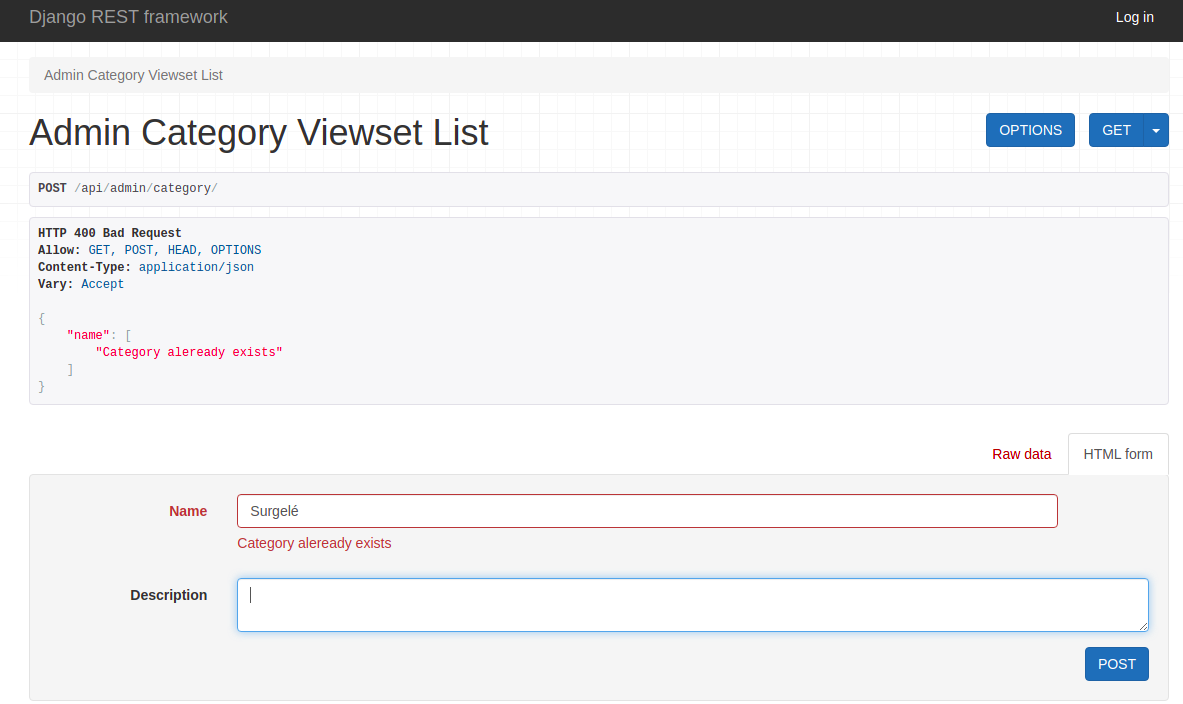
\includegraphics[width=15cm]{images/image21.png}
\end{center}
%Exemple exécutable de la vidéo
%Vous pouvez directement utiliser ce code exécutable. N'hésitez pas à l'ouvrir dans un nouvel onglet pour le modifier ou mieux voir :

%%%%%%%%%%%%%%%%%%%%%%%%%%%%%%%%%%%%%%%%%%%%%%%%%%%%%%%%

\section{Affichage et suppression pour la partie panier}
\subsection{Logique à mettre en place}
De la même manière que précédemment pour la partie {\color{monOrange}Shop}, nous souhaitons faire descendre l'information du contenu du panier le long de l'arbre des composants de cette manière :
\begin{center}
{\tt App $\to$ Cart $\to$ CartProductList $\to$ CartProduct}.
\end{center}
De cette manière, nous pourrons afficher le contenu du panier. Nous allons simplement utiliser une {\color{monOrange}prop} sur les différents niveaux de composants pour passer cette information.

Nous souhaitons également faire remonter l'information dans le sens inverse lorsque l'utilisateur clique sur le bouton "Supprimer" d'un élément du panier :

\begin{center}
{\tt CartProduct $\to$ CartProductList $\to$ Cart $\to$ App}.
\end{center}
Pour ce faire, nous allons utiliser un événement personnalisé, qui contiendra l'{\color{monOrange}id} du produit à supprimer du panier. Cet événement sera émis depuis le composant {\color{monOrange}CartProduct} concerné, puis sera réémis par {\color{monOrange}CartProductList} puis par {\color{monOrange}Cart}.

Une fois que l'événement sera arrivé au composant {\color{monOrange}App}, nous pourrons utiliser l'{\color{monOrange}id} du produit pour le supprimer du panier. La logique est donc similaire à celle utilisée pour la partie {\color{monOrange}Shop}.

\subsection{Modification de {\color{monOrange}App.vue}}
Dans {\color{monOrange}App.vue} :
\begin{minted}[
mathescape,
framesep=2mm,
baselinestretch=1.2,
fontsize=\footnotesize,
bgcolor=LightGray,
%linenos
]{html}
<script setup lang="ts">
import TheHeader from './components/Header.vue';
import TheFooter from './components/Footer.vue';
import Shop from './components/Shop/Shop.vue';
import Cart from './components/Cart/Cart.vue';
import data from './data/product';

import { reactive } from 'vue';
import type { ProductInterface } from './interfaces';

const state = reactive<{
  products: ProductInterface[];
  cart: ProductInterface[];
}>({
  products: data,
  cart: [],
});

function addProductToCart(productId: number): void {
  const product = state.products.find((product) => product.id === productId);
  if (product && !state.cart.find((product) => product.id === productId)) {
    state.cart.push({ ...product });
  }
}

function removeProductFromCart(productId: number): void {
  state.cart = state.cart.filter((product) => product.id !== productId);
}
</script>

<template>
  <div class="app-container">
    <TheHeader class="header" />
    <Shop
      :products="state.products"
      @add-product-to-cart="addProductToCart"
      class="shop"
    />
    <Cart
      :cart="state.cart"
      class="cart"
      @remove-product-from-cart="removeProductFromCart"
    />
    <TheFooter class="footer" />
  </div>
</template>

<style lang="scss">
@use './assets/base.scss' as *;
@use './assets/debug.scss' as *;

.app-container {
  min-height: 100vh;
  display: grid;
  grid-template-areas: 'header header' 'shop cart' 'footer footer';
  grid-template-columns: 75% 25%;
  grid-template-rows: 48px auto 48px;
}
.header {
  grid-area: header;
}
.shop {
  grid-area: shop;
}
.cart {
  grid-area: cart;
  border-left: var(--border);
  background-color: white;
}
.footer {
  grid-area: footer;
}
</style>
\end{minted}
Nous définissons une fonction {\color{monOrange}removeProductFromCart()} pour supprimer un article du panier lorsque nous recevons l'événement {\color{monOrange}removeProductFromCart}.
\begin{itemize}
\item {\tt @remove-product-from-cart="removeProductFromCart"} : nous écoutons l'événement {\color{monOrange}remove-product-from-cart} et enregistrons la fonction {\color{monOrange}removeProductFromCart()} comme gestionnaire d'événement.

Notez bien que nous n'utilisons pas de parenthèses avec {\color{monOrange}removeProductFromCart}. En JavaScript cela signifie que nous passons la fonction avec tous les arguments récupérés.

Notez également bien que l'événement côté {\color{monOrange}template} est en {\color{monOrange}kebab-case} ({\tt remove-product-from-cart}) et qu'il soit être en {\color{monOrange}camelCase} côté script ({\tt removeProductFromCart}).

\item {\tt :cart="state.cart" }: nous passons le contenu du panier avec une {\color{monOrange}props} au composant {\color{monOrange}Cart}.
\end{itemize}
\subsection{Modification de {\color{monOrange}Cart.vue}}
Voici le composant {\color{monOrange}Cart.vue} :
\begin{minted}[
mathescape,
framesep=2mm,
baselinestretch=1.2,
fontsize=\footnotesize,
bgcolor=LightGray,
%linenos
]{html}
<script setup lang="ts">
import CartProductList from './CartProductList.vue';
import type { ProductInterface } from '@/interfaces';

const props = defineProps<{
  cart: ProductInterface[];
}>();

const emit = defineEmits<{
  (e: 'removeProductFromCart', productId: number): void;
}>();
</script>

<template>
  <div class="p-20">
    <h2 class="mb-10">Panier</h2>
    <CartProductList
      :cart="cart"
      @remove-product-from-cart="emit('removeProductFromCart', $event)"
    />
  </div>
</template>

<style lang="scss" scoped></style>
\end{minted}
Il ne fait que transmettre dans un sens une {\color{monOrange}prop} et dans l'autre un événement. Vous pouvez le voir comme un "relais" des informations dans les deux sens.
%$
\subsection{Modification de {\color{monOrange}CartProductList.vue}}
Voici le composant :
\begin{minted}[
mathescape,
framesep=2mm,
baselinestretch=1.2,
fontsize=\footnotesize,
bgcolor=LightGray,
%linenos
]{html}
<script setup lang="ts">
import CartProduct from './CartProduct.vue';
import type { ProductInterface } from '@/interfaces';

const props = defineProps<{
  cart: ProductInterface[];
}>();

const emit = defineEmits<{
  (e: 'removeProductFromCart', productId: number): void;
}>();
</script>

<template>
  <div class="d-flex flex-column">
    <CartProduct
      v-for="product of cart"
      :product="product"
      @remove-product-from-cart="emit('removeProductFromCart', $event)"
    />
  </div>
</template>

<style lang="scss" scoped></style>
\end{minted}
Même chose, ce composant rapporte les informations dans les deux sens à chaque instance du composant {\color{monOrange}CartProduct}. Pour rappel, il y a un composant {\color{monOrange}CartProduct} pour chaque produit grâce à la directive {\color{monOrange}v-for}.
%$
\subsection{Modification de {\color{monOrange}CartProduct}}
Voici le composant :
\begin{minted}[
mathescape,
framesep=2mm,
baselinestretch=1.2,
fontsize=\footnotesize,
bgcolor=LightGray,
%linenos
]{html}
<script setup lang="ts">
import type { ProductInterface } from '@/interfaces';

defineProps<{
  product: ProductInterface;
}>();

const emit = defineEmits<{
  (e: 'removeProductFromCart', productId: number): void;
}>();
</script>

<template>
  <div class="mb-10 p-10 d-flex flex-row align-items-center product">
    <strong class="mr-10">{{ product.title }}</strong>
    <span class="mr-10">Prix : {{ product.price }}€</span>
    <button
      class="btn btn-danger"
      @click="emit('removeProductFromCart', product.id)"
    >
      Supprimer
    </button>
  </div>
</template>

<style lang="scss" scoped>
.product {
  border: var(--border);
  border-radius: var(--border-radius);
  background-color: var(--gray-1);
}
</style>
\end{minted}
Le composant émet un événement {\color{monOrange}removeProductFromCart} lorsque l'utilisateur clique sur le bouton de suppression d'un article du panier.

L'événement contient l'{\color{monOrange}id} unique du produit à supprimer.

Il affiche les informations du produit contenues dans la {\color{monOrange}prop} reçue.

%Exemple exécutable de la vidéo
%Vous pouvez directement utiliser ce code exécutable. N'hésitez pas à l'ouvrir dans un nouvel onglet pour le modifier ou mieux voir :
\begin{center}
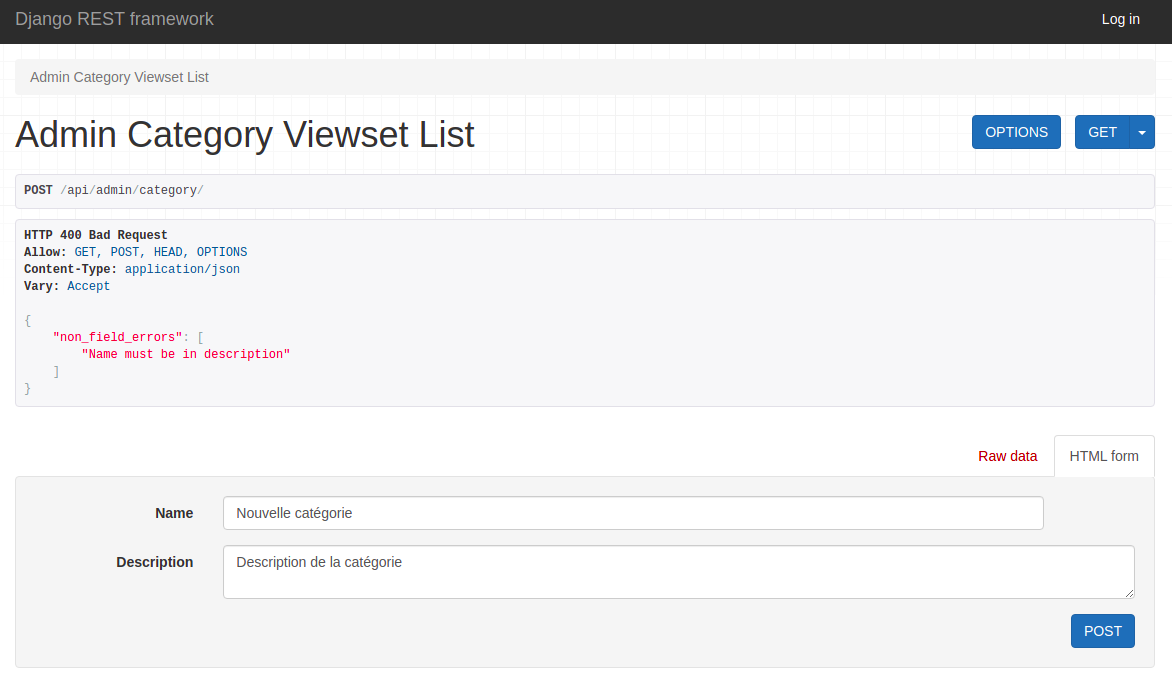
\includegraphics[width=15cm]{images/image22.png}
\end{center}
%%%%%%%%%%%%%%%%%%%%%%%%%%%%%%%%%%%%%%%%%%%%%%%%%%%%%%%%%%%%%%%

\section{Gestion des quantités}
\subsection{Création de l'interface {\color{monOrange}ProductCartInterface.ts}}
Dans le dossier {\color{monOrange}src/interfaces} crée le fichier {\color{monOrange}ProductCart.interface.ts} :
\begin{minted}[
mathescape,
framesep=2mm,
baselinestretch=1.2,
fontsize=\footnotesize,
bgcolor=LightGray,
%linenos
]{javascript}
import type { ProductInterface } from "./Product.interface";

export interface ProductCartInterface extends ProductInterface {
    quantity: number;
}
\end{minted}
La nouvelle interface étend simplement l'interface {\color{monOrange}ProductInterface} en ajoutant une propriété pour la quantité.

\subsection{Création d'un {\color{monOrange}index} pour les interfaces}
Créer un fichier {\color{monOrange}src/interfaces/index.ts} :
\begin{minted}[
mathescape,
framesep=2mm,
baselinestretch=1.2,
fontsize=\footnotesize,
bgcolor=LightGray,
%linenos
]{javascript}
export * from './Product.interface';
export * from './ProductCart.interface';
\end{minted}
Cela permet simplement de simplifier les importations des interfaces dans nos composants.

\subsection{Modification de {\color{monOrange}CartProduct.vue}}
Nous utilisons notre nouvelle interface et nous affichons la quantité de chaque produit dans le panier :
\begin{minted}[
mathescape,
framesep=2mm,
baselinestretch=1.2,
fontsize=\footnotesize,
bgcolor=LightGray,
%linenos
]{html}
<script setup lang="ts">
import type { ProductCartInterface } from '@/interfaces';

defineProps<{
  product: ProductCartInterface;
}>();

const emit = defineEmits<{
  (e: 'removeProductFromCart', productId: number): void;
}>();
</script>

<template>
  <div class="mb-10 p-10 d-flex flex-row align-items-center product">
    <strong class="mr-10">{{ product.title }}</strong>
    <span class="flex-fill mr-10">x {{ product.quantity }}</span>
    <span class="mr-10">Prix : {{ product.price }}€</span>
    <button
      class="btn btn-danger"
      @click="emit('removeProductFromCart', product.id)"
    >
      Supprimer
    </button>
  </div>
</template>

<style lang="scss" scoped>
.product {
  border: var(--border);
  border-radius: var(--border-radius);
  background-color: var(--gray-1);
}
</style>
\end{minted}
\subsection{Modification de {\color{monOrange}CartProductList.vue} et {\color{monOrange}Cart.vue}}
Utilisez la nouvelle interface :
\begin{minted}[
mathescape,
framesep=2mm,
baselinestretch=1.2,
fontsize=\footnotesize,
bgcolor=LightGray,
%linenos
]{javascript}
import type { ProductCartInterface } from '@/interfaces';

const props = defineProps<{
  cart: ProductCartInterface[];
}>();
\end{minted}
\subsection{Modification de {\color{monOrange}App.vue}}
Nous gérons maintenant l'incrémentation ou la décrémentation de la quantité lors de l'ajout ou de la suppression d'un élément du panier.

Voici le composant :
\begin{minted}[
mathescape,
framesep=2mm,
baselinestretch=1.2,
fontsize=\footnotesize,
bgcolor=LightGray,
%linenos
]{html}
<script setup lang="ts">
import TheHeader from './components/Header.vue';
import TheFooter from './components/Footer.vue';
import Shop from './components/Shop/Shop.vue';
import Cart from './components/Cart/Cart.vue';
import data from './data/product';

import { reactive } from 'vue';
import type { ProductInterface } from './interfaces';
import type { ProductCartInterface } from './interfaces';

const state = reactive<{
  products: ProductInterface[];
  cart: ProductCartInterface[];
}>({
  products: data,
  cart: [],
});

function addProductToCart(productId: number): void {
  const product = state.products.find((product) => product.id === productId);
  if (product) {
    const productInCart = state.cart.find(
      (product) => product.id === productId
    );
    if (productInCart) {
      productInCart.quantity++;
    } else {
      state.cart.push({ ...product, quantity: 1 });
    }
  }
}
function removeProductFromCart(productId: number): void {
  const productFromCart = state.cart.find(
    (product) => product.id === productId
  );
  if (productFromCart?.quantity === 1) {
    state.cart = state.cart.filter((product) => product.id !== productId);
  } else {
    productFromCart.quantity--;
  }
}
</script>

<template>
  <div class="app-container">
    <TheHeader class="header" />
    <Shop
      :products="state.products"
      @add-product-to-cart="addProductToCart"
      class="shop"
    />
    <Cart
      :cart="state.cart"
      class="cart"
      @remove-product-from-cart="removeProductFromCart"
    />
    <TheFooter class="footer" />
  </div>
</template>

<style lang="scss">
@use './assets/base.scss' as *;
@use './assets/debug.scss' as *;

.app-container {
  min-height: 100vh;
  display: grid;
  grid-template-areas: 'header header' 'shop cart' 'footer footer';
  grid-template-columns: 75% 25%;
  grid-template-rows: 48px auto 48px;
}
.header {
  grid-area: header;
}
.shop {
  grid-area: shop;
}
.cart {
  grid-area: cart;
  border-left: var(--border);
  background-color: white;
}
.footer {
  grid-area: footer;
}
</style>
\end{minted}
%Exemple exécutable de la vidéo
%Vous pouvez directement utiliser ce code exécutable. N'hésitez pas à l'ouvrir dans un nouvel onglet pour le modifier ou mieux voir :
\begin{center}
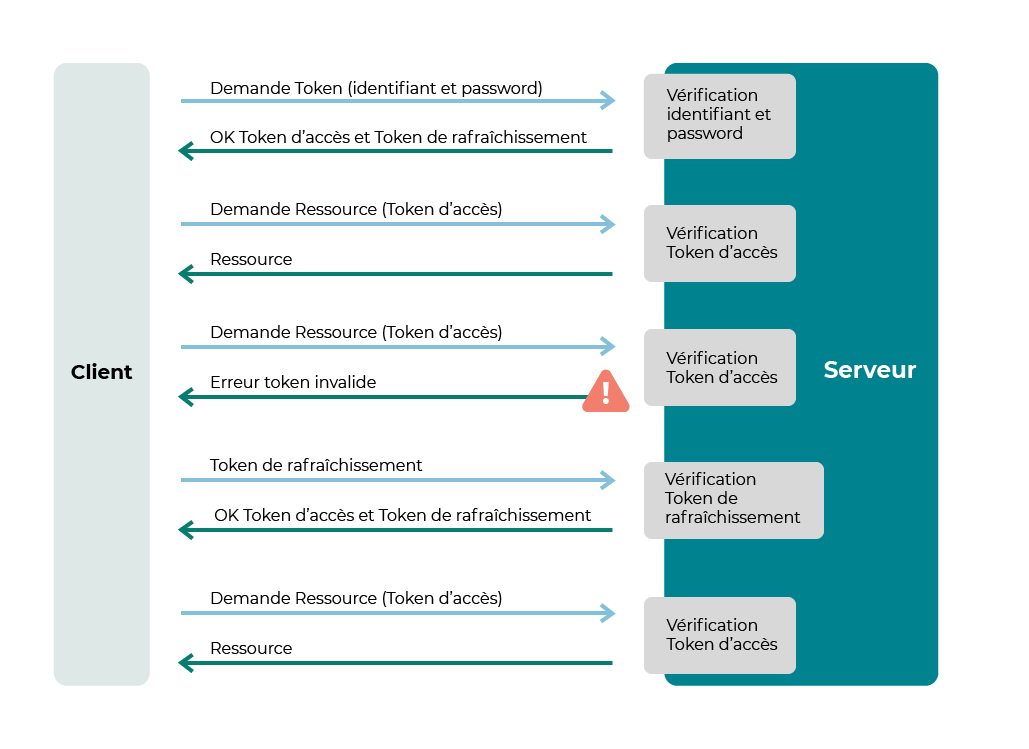
\includegraphics[width=15cm]{images/image23.png}
\end{center}
%%%%%%%%%%%%%%%%%%%%%%%%%%%%%%%%%%%%%%%%%%%%%%%%%%%%%%%%%%%%%%%%

\section{Affichage du total et affichage initial du panier}
\subsection{Création dossier pour les styles}
Dans le dossier {\color{monOrange}assets}, créez un dossier {\color{monOrange}scss} et placez-y les fichiers {\color{monOrange}base.scss} et {\color{monOrange}debug.scss}. N'oubliez pas de modifier en conséquence les importations dans {\color{monOrange}App.vue} :
\begin{minted}[
mathescape,
framesep=2mm,
baselinestretch=1.2,
fontsize=\footnotesize,
bgcolor=LightGray,
%linenos
]{html}
<style lang="scss">
@use './assets/scss/base.scss' as *;
@use './assets/scss/debug.scss' as *;
\end{minted}

\subsection{Ajout d'une classe}
Dans le fichier {\color{monOrange}base.scss}, ajoutez la classe suivante :
\begin{minted}[
mathescape,
framesep=2mm,
baselinestretch=1.2,
fontsize=\footnotesize,
bgcolor=LightGray,
%linenos
]{scss}
.btn-success {
    background-color: var(--success-1);
    color: var(--text-primary-color);
    &:hover {
        background-color: var(--success-2);
    }
}
\end{minted}
\subsection{Modification de {\color{monOrange}Cart.vue}}
Nous utilisons une propriété utilisée pour calculer le total du panier :
\begin{minted}[
mathescape,
framesep=2mm,
baselinestretch=1.2,
fontsize=\footnotesize,
bgcolor=LightGray,
%linenos
]{html}
<script setup lang="ts">
import type { ProductCartInterface } from '@/interfaces';
import { computed } from 'vue';
import CartProductList from './CartProductList.vue';
const props = defineProps<{
  cart: ProductCartInterface[];
}>();
const totalPrice = computed(() =>
  props.cart.reduce((acc, product) => acc + product.price * product.quantity, 0)
);
const emit = defineEmits<{
  (e: 'removeProductFromCart', productId: number): void;
}>();
</script>

<template>
  <div class="p-20 d-flex flex-column">
    <h2 class="mb-10">Panier</h2>
    <CartProductList
      class="flex-fill"
      :cart="cart"
      @remove-product-from-cart="emit('removeProductFromCart', $event)"
    />
    <button class="btn btn-success">Commander ({{ totalPrice }}€)</button>
  </div>
</template>

<style lang="scss" scoped></style>
\end{minted} 
\subsection{Modification de {\color{monOrange}App.vue}}
Nous utilisons une propriété exploitée pour calculer pour savoir si le panier est vide ou non. Si le panier est vide, nous n'affichons pas le composant panier grâce à la directive {\color{monOrange}v-if}. Nous utilisons également une liaison de classe avec la directive {\color{monOrange}v-bind} pour appliquer la classe {\color{monOrange}gridEmpty} si le panier est vide. Cette classe permet de modifier simplement la grille {\color{monOrange}CSS}.
\begin{minted}[
mathescape,
framesep=2mm,
baselinestretch=1.2,
fontsize=\footnotesize,
bgcolor=LightGray,
%linenos
]{html}
<script setup lang="ts">
import TheHeader from './components/Header.vue';
import TheFooter from './components/Footer.vue';
import Shop from './components/Shop/Shop.vue';
import Cart from './components/Cart/Cart.vue';
import data from './data/product';

import { computed, reactive } from 'vue';
import type { ProductInterface } from './interfaces';
import type { ProductCartInterface } from './interfaces';

const state = reactive<{
  products: ProductInterface[];
  cart: ProductCartInterface[];
}>({
  products: data,
  cart: [],
});

function addProductToCart(productId: number): void {
  const product = state.products.find((product) => product.id === productId);
  if (product) {
    const productInCart = state.cart.find(
      (product) => product.id === productId
    );
    if (productInCart) {
      productInCart.quantity++;
    } else {
      state.cart.push({ ...product, quantity: 1 });
    }
  }
}

function removeProductFromCart(productId: number): void {
  const productFromCart = state.cart.find(
    (product) => product.id === productId
  );
  if (productFromCart?.quantity === 1) {
    state.cart = state.cart.filter((product) => product.id !== productId);
  } else {
    productFromCart.quantity--;
  }
}

const cartEmpty = computed(() => state.cart.length === 0);
</script>

<template>
  <div
    class="app-container"
    :class="{
      gridEmpty: cartEmpty,
    }"
  >
    <TheHeader class="header" />
    <Shop
      :products="state.products"
      @add-product-to-cart="addProductToCart"
      class="shop"
    />
    <Cart
      v-if="!cartEmpty"
      :cart="state.cart"
      class="cart"
      @remove-product-from-cart="removeProductFromCart"
    />
    <TheFooter class="footer" />
  </div>
</template>

<style lang="scss">
@use './assets/base.scss' as *;
@use './assets/debug.scss' as *;

.app-container {
  min-height: 100vh;
  display: grid;
  grid-template-areas: 'header header' 'shop cart' 'footer footer';
  grid-template-columns: 75% 25%;
  grid-template-rows: 48px auto 48px;
}

.gridEmpty {
  grid-template-areas: 'header' 'shop' 'footer';
  grid-template-columns: 100%;
}

.header {
  grid-area: header;
}

.shop {
  grid-area: shop;
}

.cart {
  grid-area: cart;
  border-left: var(--border);
  background-color: white;
}

.footer {
  grid-area: footer;
}
</style>
\end{minted}
%Exemple exécutable de la vidéo
%Vous pouvez directement utiliser ce code exécutable. N'hésitez pas à l'ouvrir dans un nouvel onglet pour le modifier ou mieux voir :

\begin{center}
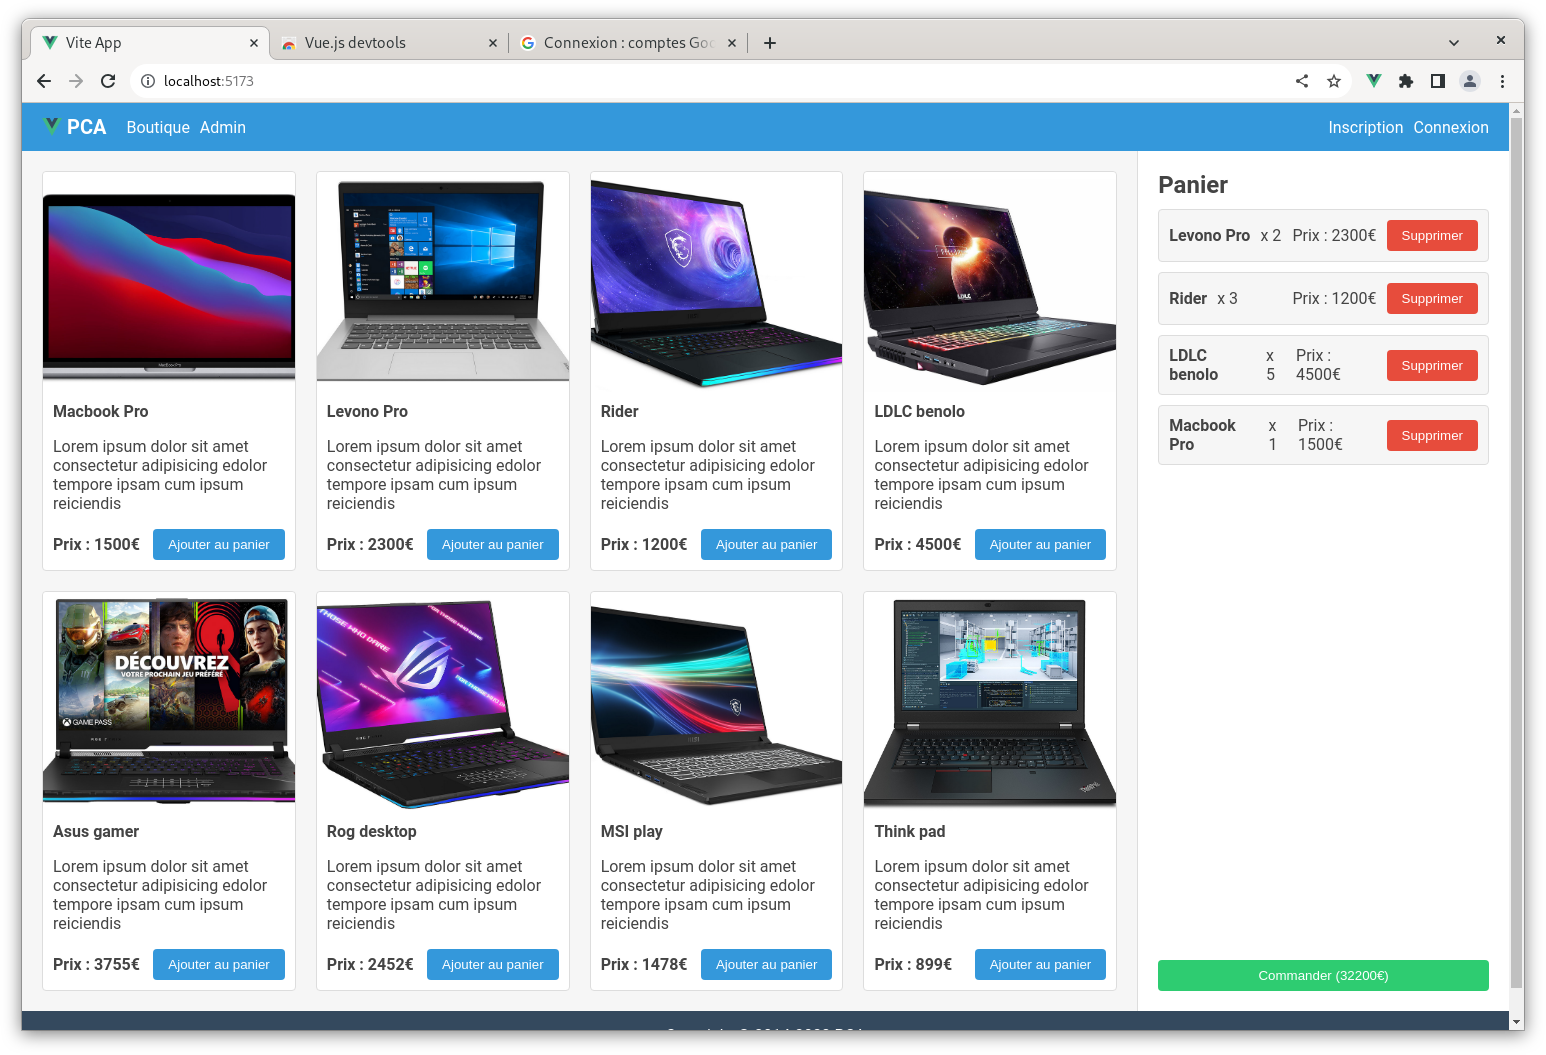
\includegraphics[width=15cm]{images/image24.png}
\end{center}
	\chapter{Projet Boutique - partie 2}
	\section{ Introduction et objectifs}
\subsection{Objectifs}
Nous repartons du projet où nous l'avons laissé. Nous allons ajouter des filtres pour notre boutique : une barre de recherche, un filtre par prix et un filtre par catégorie.

\subsection{Création de l'interface pour nos filtres}
Dans le dossier {\tt interfaces}, créez le fichier {\tt Filters.interface.ts} :
\begin{minted}[
mathescape,
framesep=2mm,
baselinestretch=1.2,
fontsize=\footnotesize,
bgcolor=LightGray,
%linenos
]{javascript}
export type Category = 'gamer' | 'desktop' | 'streaming' | 'all';

export interface FiltersInterface {
  search: string;
  priceRange: [number, number];
  category: Category;
}
\end{minted}
Modifiez ensuite les {\color{monOrange}exports} de l'{\tt index} :
\begin{minted}[
mathescape,
framesep=2mm,
baselinestretch=1.2,
fontsize=\footnotesize,
bgcolor=LightGray,
%linenos
]{javascript}
export * from './Product.interface';
export * from './ProductCart.interface';
export * from './Filters.interface';
\end{minted}
\subsection{Modification de {\color{monOrange}App.vue}}
Nous modifions le {\color{monOrange}state} réactif de notre composant racine, en ajoutant une propriété qui contient les filtres en cours. Nous avons des filtres sélectionnés par défaut contenus dans {\tt DEFAULT\_FILTERS}.
\begin{minted}[
mathescape,
framesep=2mm,
baselinestretch=1.2,
fontsize=\footnotesize,
bgcolor=LightGray,
%linenos
]{javascript}
<script setup lang="ts">
import TheHeader from './components/Header.vue';
import TheFooter from './components/Footer.vue';
import Shop from './components/Shop/Shop.vue';
import Cart from './components/Cart/Cart.vue';
import data from './data/product';
import { DEFAULT_FILTERS } from './data/filters';
import { computed, reactive } from 'vue';
import type {
  FiltersInterface,
  ProductCartInterface,
  ProductInterface,
} from './interfaces';

const state = reactive<{
  products: ProductInterface[];
  cart: ProductCartInterface[];
  filters: FiltersInterface;
}>({
  products: data,
  cart: [],
  filters: DEFAULT_FILTERS,
});
// …
\end{minted}
\subsection{Création du fichier {\tt data/filters.ts}}
Nous exportons nos filtres par défaut dans une constante :
\begin{minted}[
mathescape,
framesep=2mm,
baselinestretch=1.2,
fontsize=\footnotesize,
bgcolor=LightGray,
%linenos
]{javascript}
import type { FiltersInterface } from '../interfaces';

export const DEFAULT_FILTERS: FiltersInterface = {
  search: '',
  priceRange: [0, 10000],
  category: 'all',
};
\end{minted}
\subsection{Modification de l'interface Product}
Modifiez le fichier {\tt interfaces/ProductInterface.ts} pour ajouter une propriété {\color{monOrange}category} :
\begin{minted}[
mathescape,
framesep=2mm,
baselinestretch=1.2,
fontsize=\footnotesize,
bgcolor=LightGray,
%linenos
]{javascript}
import type { Category } from './Filters.interface';

export interface ProductInterface {
  id: number;
  title: string;
  image: string;
  price: number;
  description: string;
  category: Category;
}
\end{minted}
\subsection{Modification de data/products}
Il faut ajouter ensuite une catégorie à nos produits en dur :
\begin{minted}[
mathescape,
framesep=2mm,
baselinestretch=1.2,
fontsize=\footnotesize,
bgcolor=LightGray,
%linenos
]{javascript}
import type { ProductInterface } from "@/interfaces";

export default [
    {
        id: 1,
        image: 'src/assets/images/macbookpro.PNG',
        title: 'Macbook Pro',
        description: 'Lorem ipsum dolor sit amet consectetur adipisicing edolor tempore ipsam cum ipsum reiciendis',
        price: 1500,
        category: 'desktop'
    },
    {
        id: 2,
        image: 'src/assets/images/levono.PNG',
        title: 'Levono Pro',
        description: 'Lorem ipsum dolor sit amet consectetur adipisicing edolor tempore ipsam cum ipsum reiciendis',
        price: 2300,
        category: 'desktop'
    },
    {
        id: 3,
        image: 'src/assets/images/rider.PNG',
        title: 'Rider',
        description: 'Lorem ipsum dolor sit amet consectetur adipisicing edolor tempore ipsam cum ipsum reiciendis',
        price: 1200,
        category: 'gamer'
    },
    {
        id: 4,
        image: 'src/assets/images/ldlc.PNG',
        title: 'LDLC benolo',
        description: 'Lorem ipsum dolor sit amet consectetur adipisicing edolor tempore ipsam cum ipsum reiciendis',
        price: 4500,
        category: 'streaming'
    },
    {
        id: 5,
        image: 'src/assets/images/asus.PNG',
        title: 'Asus gamer',
        description: 'Lorem ipsum dolor sit amet consectetur adipisicing edolor tempore ipsam cum ipsum reiciendis',
        price: 3755,
        category: 'gamer'
    },
    {
        id: 6,
        image: 'src/assets/images/rog.PNG',
        title: 'Rog desktop',
        description: 'Lorem ipsum dolor sit amet consectetur adipisicing edolor tempore ipsam cum ipsum reiciendis',
        price: 2452,
        category: 'streaming'
    },
    {
        id: 7,
        image: 'src/assets/images/msi.PNG',
        title: 'MSI play',
        description: 'Lorem ipsum dolor sit amet consectetur adipisicing edolor tempore ipsam cum ipsum reiciendis',
        price: 1478,
        category: 'gamer'
    },
    {
        id: 8,
        image: 'src/assets/images/pad.PNG',
        title: 'Think pad',
        description: 'Lorem ipsum dolor sit amet consectetur adipisicing edolor tempore ipsam cum ipsum reiciendis',
        price: 899,
        category: 'desktop'
    },
] as ProductInterface[]
\end{minted}
Code de la vidéo
Voici le code de la vidéo :

%%%%%%%%%%%%%%%%%%%%%%%%%%%%%%%%%%%%%%%%%%%%%%%%%%%%%%%%%%%%%%%%%%%%%

\section{Préparation pour le filtrage des produits}
\subsection{Modification de ShopProductList.vue}
Nous ajoutons une {\color{monOrange}key} pour la directive {\color{monOrange}v-for} afin d'optimiser les performances de mise à jour des produits :
\begin{minted}[
mathescape,
framesep=2mm,
baselinestretch=1.2,
fontsize=\footnotesize,
bgcolor=LightGray,
%linenos
]{html}
<script setup lang="ts">
import type { ProductInterface } from '@/interfaces';
import ShopProduct from './ShopProduct.vue';

defineProps<{
  products: ProductInterface[];
}>();

const emit = defineEmits<{
  (e: 'addProductToCart', productId: number): void;
}>();
</script>

<template>
  <div class="grid p-20">
    <ShopProduct
      @add-product-to-cart="emit('addProductToCart', $event)"
      v-for="product of products"
      :product="product"
      :key="product.id"
    />
  </div>
</template>

<style lang="scss" scoped>
.grid {
  display: grid;
  grid-template-columns: 1fr 1fr 1fr 1fr;
  grid-auto-rows: 400px;
  gap: 20px;
}
</style>
\end{minted}
%$
\subsection{Modification de Filters.interface.ts}
Nous allons ajouter une interface {\tt FilterUpdate} :
\begin{minted}[
mathescape,
framesep=2mm,
baselinestretch=1.2,
fontsize=\footnotesize,
bgcolor=LightGray,
%linenos
]{javascript}
export type Category = 'gamer' | 'desktop' | 'streaming' | 'all';

export interface FiltersInterface {
  search: string;
  priceRange: [number, number];
  category: Category;
}

export interface FilterUpdate {
  search?: string;
  priceRange?: [number, number];
  category?: Category;
}
\end{minted}
{\tt FilterUpdate} contiendra le filtre appliqués par l'utilisateur à chaque fois qu'il modifie un filtre. Ainsi par exemple, s'il modifie l'intervalle de prix, l'objet contiendra {\tt priceRange} uniquement. Même chose s'il effectue une recherche, nous aurons la propriété {\color{monOrange}search} uniquement. C'est pour cette raison que toutes les propriétés sont optionnelles avec {\color{monOrange}?}.

\subsection{Modification de {\tt App.vue}}
Nous filtrons les produits à afficher en fonction de toutes les options des filtres que nous allons mettre en place en utilisant une propriété calculée. Nous écoutons l'événement que nous allons émettre lorsque l'utilisateur modifiera un filtre et nous modifions l'état des filtres en fonction de l'événement reçu.
\begin{minted}[
mathescape,
framesep=2mm,
baselinestretch=1.2,
fontsize=\footnotesize,
bgcolor=LightGray,
%linenos
]{html}
<script setup lang="ts">
import TheHeader from './components/Header.vue';
import TheFooter from './components/Footer.vue';
import Shop from './components/Shop/Shop.vue';
import Cart from './components/Cart/Cart.vue';
import data from './data/product';
import { computed, reactive } from 'vue';
import type {
  FiltersInterface,
  ProductCartInterface,
  ProductInterface,
  FilterUpdate,
} from './interfaces';
import { DEFAULT_FILTERS } from './data/filters';

const state = reactive<{
  products: ProductInterface[];
  cart: ProductCartInterface[];
  filters: FiltersInterface;
}>({
  products: data,
  cart: [],
  filters: { ...DEFAULT_FILTERS },
});

function addProductToCart(productId: number): void {
  const product = state.products.find((product) => product.id === productId);
  if (product) {
    const productInCart = state.cart.find(
      (product) => product.id === productId
    );
    if (productInCart) {
      productInCart.quantity++;
    } else {
      state.cart.push({ ...product, quantity: 1 });
    }
  }
}

function removeProductFromCart(productId: number): void {
  const productFromCart = state.cart.find(
    (product) => product.id === productId
  );
  if (productFromCart?.quantity === 1) {
    state.cart = state.cart.filter((product) => product.id !== productId);
  } else {
    productFromCart.quantity--;
  }
}

function updateFilter(filterUpdate: FilterUpdate) {
  if (filterUpdate.search !== undefined) {
    state.filters.search = filterUpdate.search;
  } else if (filterUpdate.priceRange) {
    state.filters.priceRange = filterUpdate.priceRange;
  } else if (filterUpdate.category) {
    state.filters.category = filterUpdate.category;
  } else {
    state.filters = { ...DEFAULT_FILTERS };
  }
}

const cartEmpty = computed(() => state.cart.length === 0);

const filteredProducts = computed(() => {
  return state.products.filter((product) => {
    if (
      product.title
        .toLocaleLowerCase()
        .startsWith(state.filters.search.toLocaleLowerCase()) &&
      product.price >= state.filters.priceRange[0] &&
      product.price <= state.filters.priceRange[1] &&
      (product.category === state.filters.category ||
        state.filters.category === 'all')
    ) {
      return true;
    } else {
      return false;
    }
  });
});
</script>

<template>
  <div
    class="app-container"
    :class="{
      gridEmpty: cartEmpty,
    }"
  >
    <TheHeader class="header" />
    <Shop
      @update-filter="updateFilter"
      :products="filteredProducts"
      @add-product-to-cart="addProductToCart"
      class="shop"
    />
    <Cart
      v-if="!cartEmpty"
      :cart="state.cart"
      class="cart"
      @remove-product-from-cart="removeProductFromCart"
    />
    <TheFooter class="footer" />
  </div>
</template>
\end{minted}
Notez bien que nous passons maintenant la propriété calculée {\tt filteredProducts} à notre composant Shop et non plus les produits du {\color{monOrange}state}.

Notez également que {\tt \{ ...DEFAULT\_FILTERS \} } permet de créer un nouvel objet différent lors de la réinitialisation des filtres pour ne pas avoir le même objet que dans le {\color{monOrange}state}.

\subsection{Code de la vidéo}
Voici le code de la vidéo :

%%%%%%%%%%%%%%%%%%%%%%%%%%%%%%%%%%%%%%%%%%%%%%%%%%%%%%%%%%%%%%%%%%%%%
\section{Création du composant ShopFilters}
\subsection{Création du composantShopFilters}
Dans le dossier {\tt src/shop} créez le fichier {\tt ShopFilters.vue}. Ce sera le composant responsable des filtres de l’application.

\subsection{Modification deApp.vue}
Nous passons en {\color{monOrange}prop} les filtres à notre composant {\color{monOrange}Shop} pour que celui-ci puisse les passer ensuite au composant responsable des filtres.
\begin{minted}[
mathescape,
framesep=2mm,
baselinestretch=1.2,
fontsize=\footnotesize,
bgcolor=LightGray,
%linenos
]{html}
<template>
  <div
    class="app-container"
    :class="{
      gridEmpty: cartEmpty,
    }"
  >
    <TheHeader class="header" />
    <Shop
      @update-filter="updateFilter"
      :products="filteredProducts"
      :filters="state.filters"
      @add-product-to-cart="addProductToCart"
      class="shop"
    />
    <!-- ..... -->
\end{minted}
\subsection{Modification de Shop.vue}
Nous modifions le composant {\tt Shop.vue} qui va recevoir en {\color{monOrange}prop} les filtres depuis le composant {\tt App.vue}. Il les repasse ensuite au composant {\tt ShopFilters}. Il va également ré-émettre l'événement {\tt updateFilter} qu'il va recevoir du composant {\tt ShopFilters} pour mettre à jour le filtre modifié par l'utilisateur. Ici il ne fait donc que transmettre l'événement et les {\color{monOrange}props} dans les deux sens entre {\tt App.vue} et {\tt ShopFilters}.
\begin{minted}[
mathescape,
framesep=2mm,
baselinestretch=1.2,
fontsize=\footnotesize,
bgcolor=LightGray,
%linenos
]{html}
<script setup lang="ts">
import type {
  FiltersInterface,
  ProductInterface,
  FilterUpdate,
} from '../../interfaces';
import ShopProductList from './ShopProductList.vue';
import ShopFilters from './ShopFilters.vue';

defineProps<{
  products: ProductInterface[];
  filters: FiltersInterface;
}>();

const emit = defineEmits<{
  (e: 'addProductToCart', productId: number): void;
  (e: 'updateFilter', updateFilter: FilterUpdate): void;
}>();
</script>

<template>
  <div class="d-flex flex-row">
    <ShopFilters
      :filters="filters"
      @update-filter="emit('updateFilter', $event)"
      class="shop-filter"
    />
    <ShopProductList
      class="flex-fill"
      @add-product-to-cart="emit('addProductToCart', $event)"
      :products="products"
    />
  </div>
</template>

<style lang="scss" scoped>
.shop-filter {
  flex: 0 0 200px;
}
</style>
\end{minted}
\subsection{Modification de {\tt ShopFilters.vue}}
Nous mettons en place le composant en créant le premier filtre pour la recherche par nom de produit. Lorsque l'utilisateur tape dans le champ de la recherche, il va émettre un événement {\tt updateFilter} avec la valeur du champ.
\begin{minted}[
mathescape,
framesep=2mm,
baselinestretch=1.2,
fontsize=\footnotesize,
bgcolor=LightGray,
%linenos
]{html}
<script setup lang="ts">
import type { FiltersInterface, FilterUpdate } from '../../interfaces';
defineProps<{
  filters: FiltersInterface;
}>();
const emit = defineEmits<{
  (e: 'updateFilter', filterUpdate: FilterUpdate): void;
}>();
</script>

<template>
  <div class="p-20 d-flex flex-column">
    <section class="mb-20">
      <h3 class="mb-10">Rechercher</h3>
      <input
        :value="filters.search"
        @input="emit('updateFilter', { search: ($event.target as HTMLInputElement).value })"
        type="text"
        placeholder="Rechercher"
      />
    </section>
  </div>
</template>

<style lang="scss" scoped></style>
\end{minted}

% $%Code de la vidéo 
%Voici le code de la vidéo :

\begin{center}
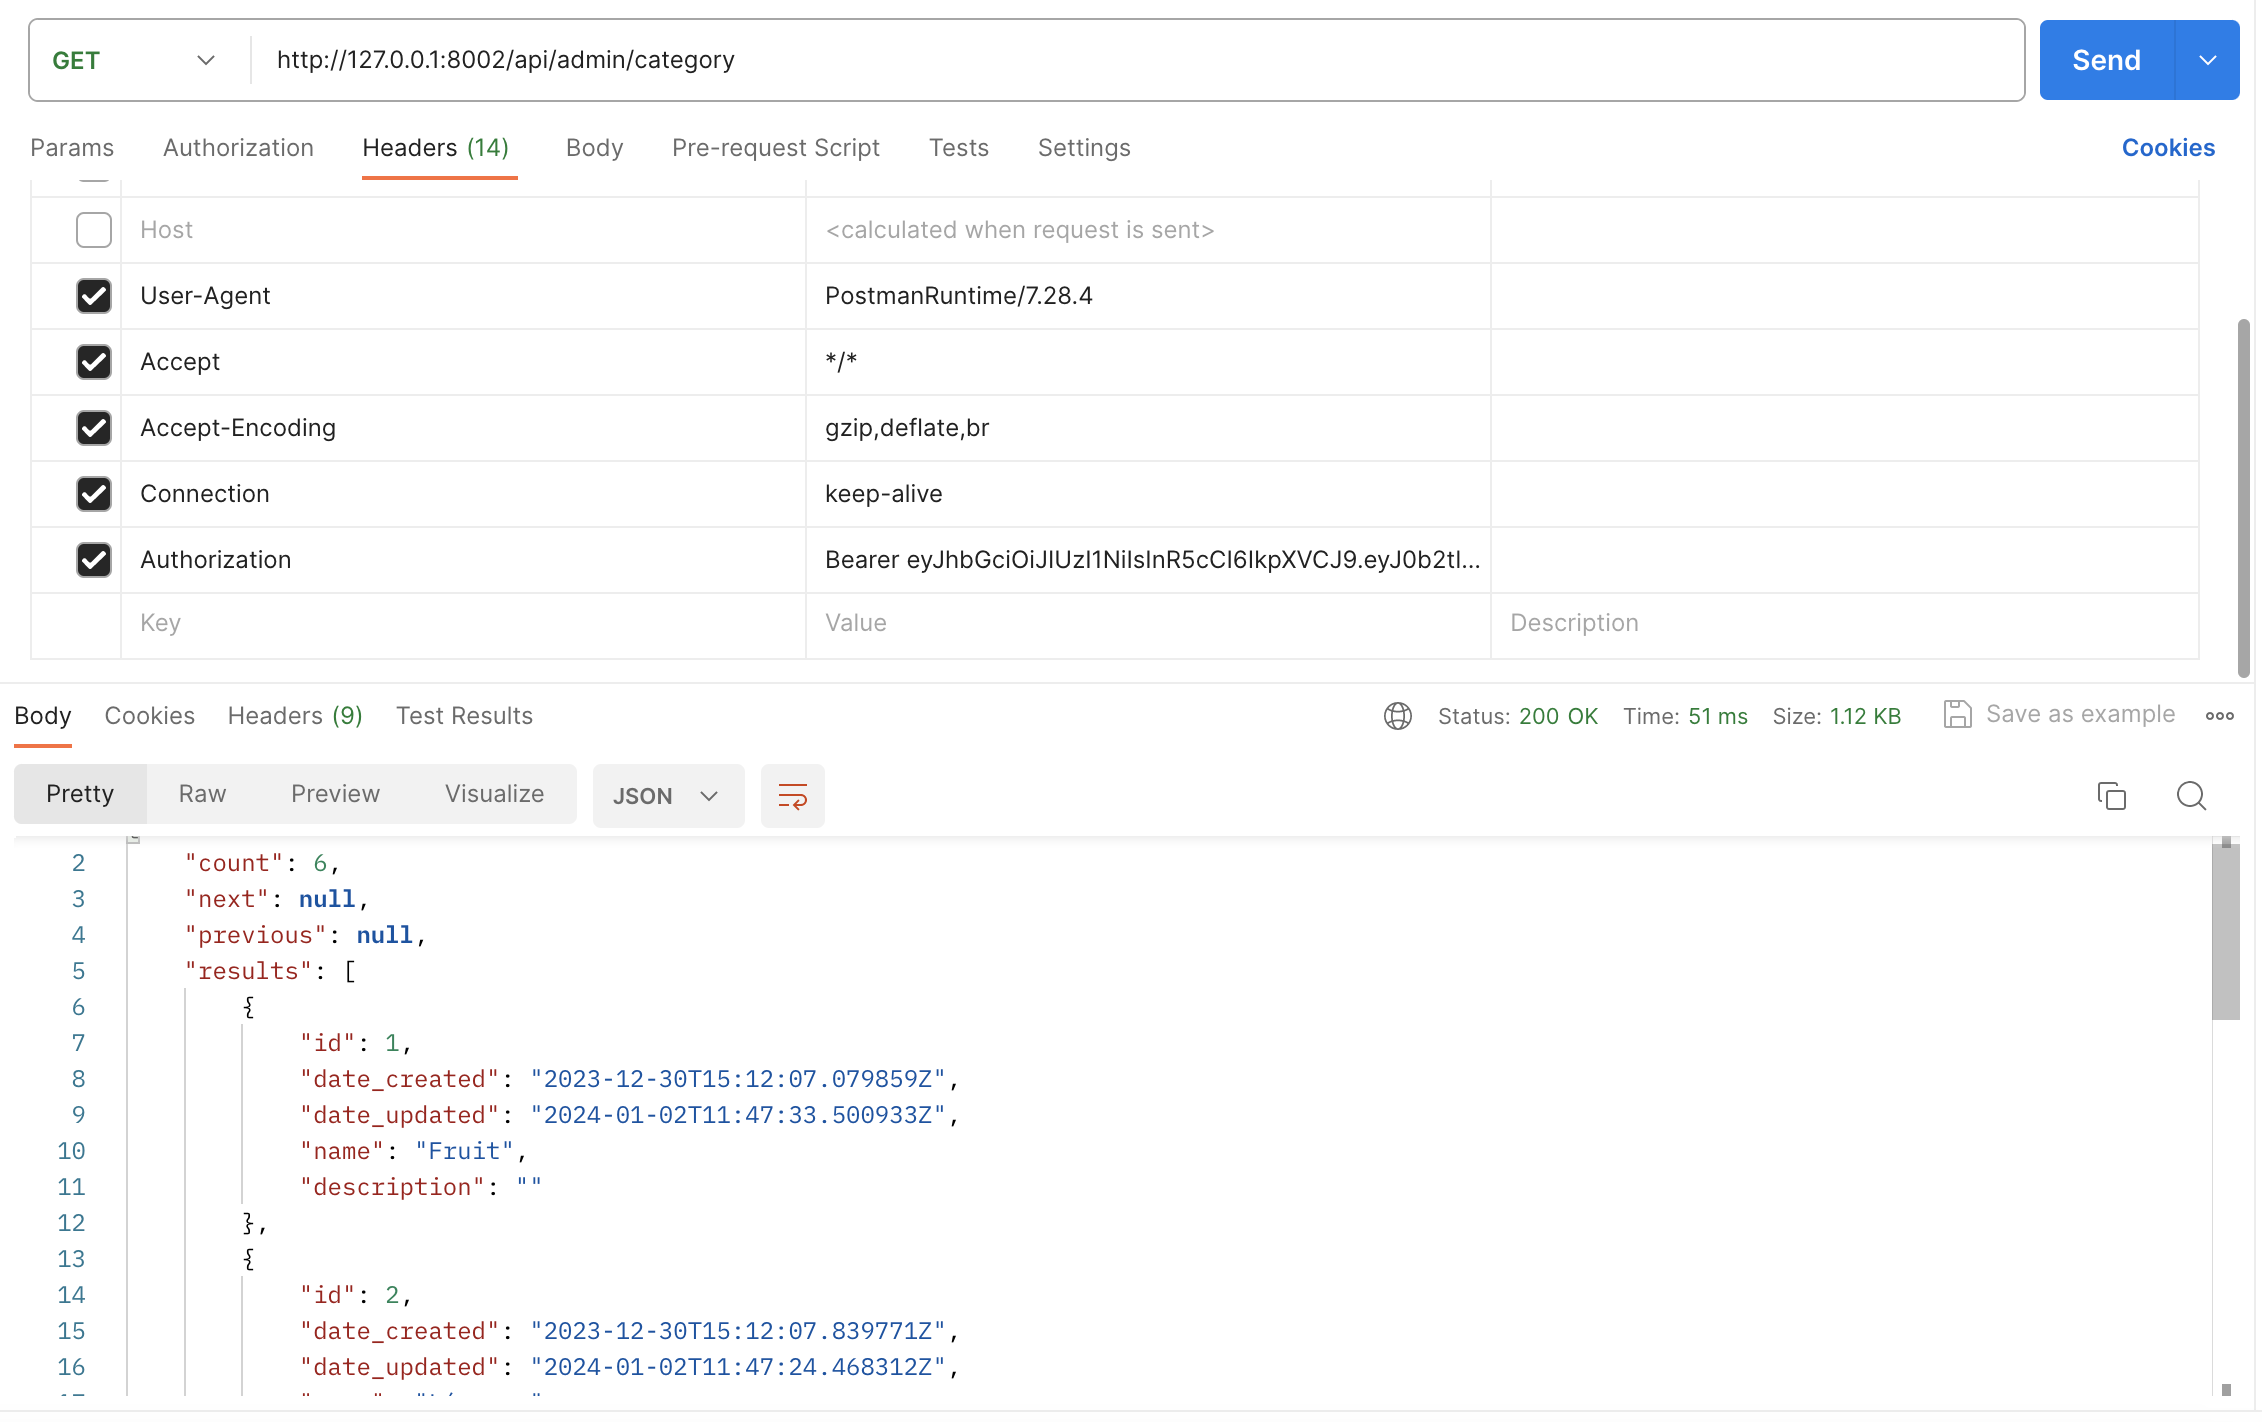
\includegraphics[width=15cm]{images/image25.png}
\end{center}
%%%%%%%%%%%%%%%%%%%%%%%%%%%%%%%%%%%%%%%%%%%%%%%%%%%%%%%%%%%%%%%%%%%%%

\section{Filtrer les produits par prix}
\subsection{Modification de {\tt ShopFilters.vue}}
Nous ajoutons le filtre par intervalles de prix :
\begin{minted}[
mathescape,
framesep=2mm,
baselinestretch=1.2,
fontsize=\footnotesize,
bgcolor=LightGray,
%linenos
]{html}
<script setup lang="ts">
import type { FiltersInterface, FilterUpdate } from '../../interfaces';
defineProps<{
  filters: FiltersInterface;
}>();
const emit = defineEmits<{
  (e: 'updateFilter', filterUpdate: FilterUpdate): void;
}>();
</script>

<template>
  <div class="p-20 d-flex flex-column">
    <section class="mb-20">
      <h3 class="mb-10">Rechercher</h3>
      <input
        :value="filters.search"
        @input="emit('updateFilter', { search: ($event.target as HTMLInputElement).value })"
        type="text"
        placeholder="Rechercher"
      />
    </section>
    <section class="mb-20">
      <h3 class="mb-10">Trier par prix</h3>
      <div
        class="mb-5"
        v-for="priceRange of ([[0, 10000], [800, 1000], [1000, 1500], [1500, 2000], [2000, 10000]] as [number, number][])"
      >
        <input
          :checked="filters.priceRange[0] === priceRange[0]"
          type="radio"
          @input="emit('updateFilter', { priceRange })"
          name="priceRange"
          :id="priceRange[0].toString()"
        />
        <label :for="priceRange[0].toString()">
          {{
            priceRange[0] === 0
              ? 'Tous les prix'
              : priceRange[0] === 2000
              ? 'Plus de 2000€'
              : `Entre ${priceRange[0]}€ et ${priceRange[1]}€`
          }}
        </label>
      </div>
    </section>
  </div>
</template>

<style lang="scss" scoped></style>
\end{minted}

%$
\begin{itemize}
\item {\color{monOrange} as [number, number][]:} permet de préciser à TypeScriptque nous avons bien un tableau contenant des tableaux avec exactement deux éléments de type nombre.

\item {\color{monOrange} v-for="priceRange of:} permet d'itérer sur l'ensemble des intervalles de prix.

\item {\color{monOrange} :checked="filters.priceRange[0] === priceRange[0]":} nous cochons l'élément uniquement si la valeur minimale de l'intervalle contenue dans les filtres passés est la même que la valeur minimale de l'intervalle de l'itération en cours.

\item {\color{monOrange} @input="emit('updateFilter', { priceRange })": } permet d'émettre l'événement de mise à jour des filtres avec en valeur un objet contenant une propriété qui a en clé le filtre à modifier et en valeur l'intervalle sélectionné.

\item {\color{monOrange} :id="priceRange[0].toString()":} nous nous servions de la valeur Inférieure de l'intervalle comme identifiant HTMLunique.

\end{itemize}
\subsection{Code de la vidéo}
Voici le code de la vidéo :

\begin{center}
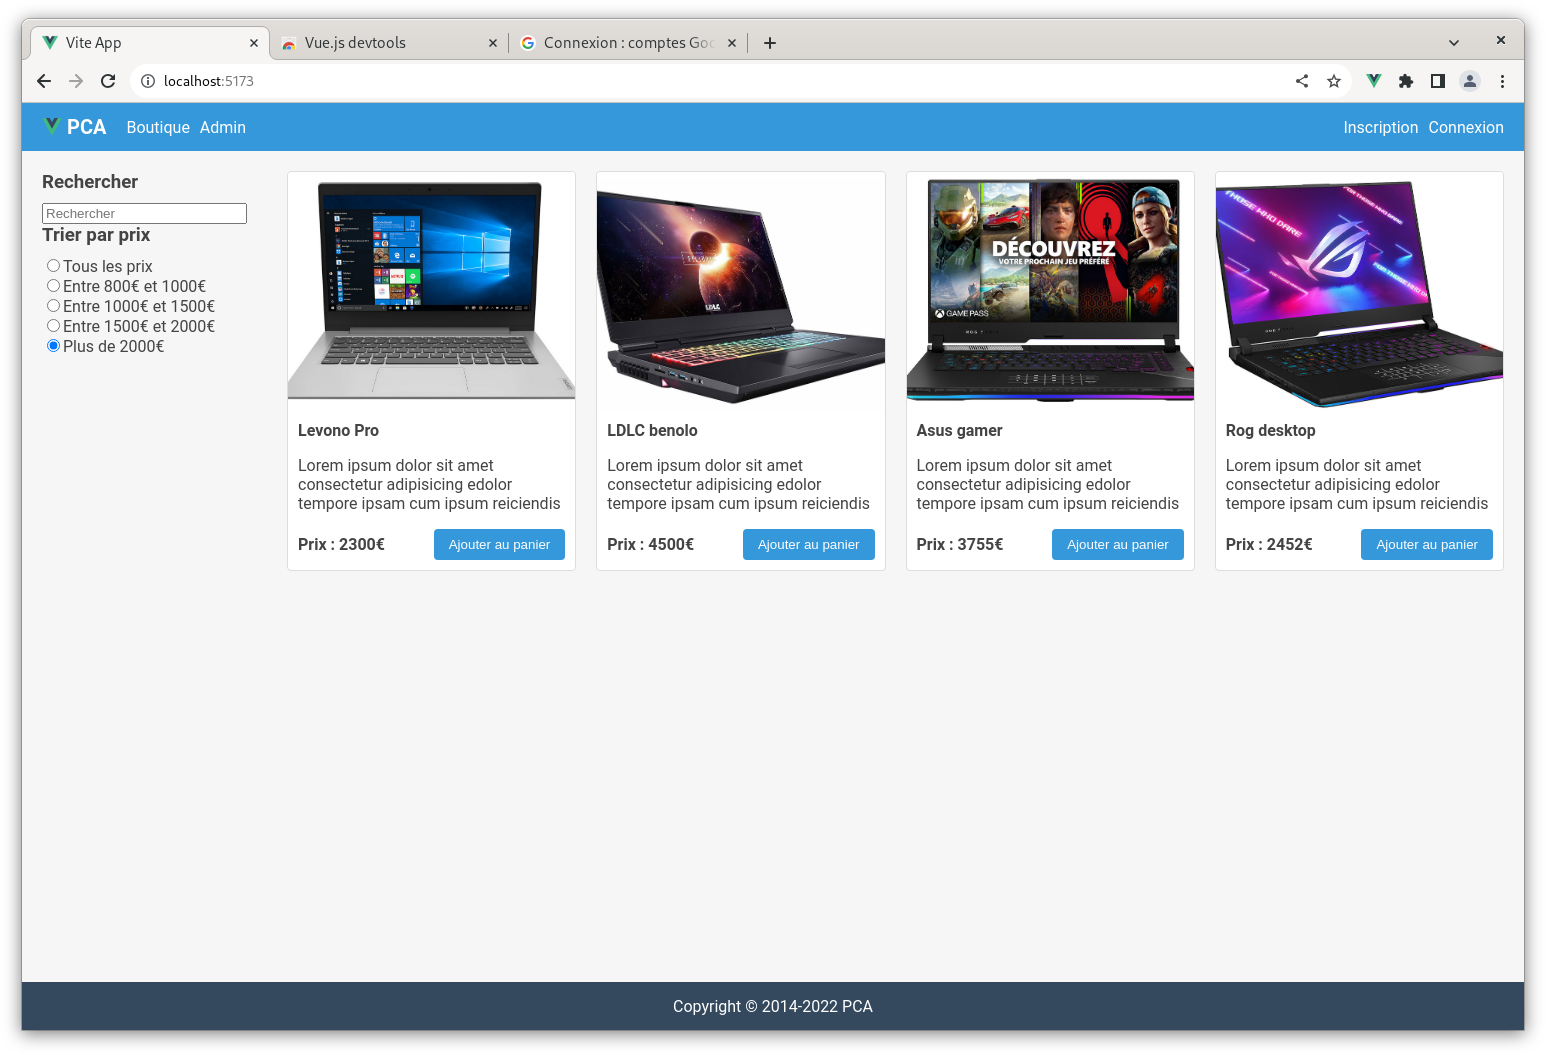
\includegraphics[width=15cm]{images/image26.png}
\end{center}

%%%%%%%%%%%%%%%%%%%%%%%%%%%%%%%%%%%%%%%%%%%%%%%%%%%%%%%%%%%%%%%%%%%%%%%
\section{Filtrer les produits par catégorie}
\subsection{Modification de {\tt ShopFilters.vue}}
Nous ajoutons le filtre par catégorie :
\begin{minted}[
mathescape,
framesep=2mm,
baselinestretch=1.2,
fontsize=\footnotesize,
bgcolor=LightGray,
%linenos
]{html}
<script setup lang="ts">
import type {
  FiltersInterface,
  FilterUpdate,
  Category,
} from '../../interfaces';
defineProps<{
  filters: FiltersInterface;
}>();
const emit = defineEmits<{
  (e: 'updateFilter', filterUpdate: FilterUpdate): void;
}>();
</script>

<template>
  <div class="p-20 d-flex flex-column">
    <section class="mb-20">
      <h3 class="mb-10">Rechercher</h3>
      <input
        :value="filters.search"
        @input="emit('updateFilter', { search: ($event.target as HTMLInputElement).value })"
        type="text"
        placeholder="Rechercher"
      />
    </section>
    <section class="mb-20">
      <h3 class="mb-10">Trier par prix</h3>
      <div
        class="mb-5"
        v-for="priceRange of ([[0, 10000], [800, 1000], [1000, 1500], [1500, 2000], [2000, 10000]] as [number, number][])"
      >
        <input
          :checked="filters.priceRange[0] === priceRange[0]"
          type="radio"
          @input="emit('updateFilter', { priceRange })"
          name="priceRange"
          :id="priceRange[0].toString()"
        />
        <label :for="priceRange[0].toString()">
          {{
            priceRange[0] === 0
              ? 'Tous les prix'
              : priceRange[0] === 2000
              ? 'Plus de 2000€'
              : `Entre ${priceRange[0]}€ et ${priceRange[1]}€`
          }}
        </label>
      </div>
    </section>
    <section class="mb-20 flex-fill">
      <h3 class="mb-10">Trier par categories</h3>
      <p
        class="category"
        :class="{ selected: filters.category === category }"
        v-for="category in (['all', 'desktop', 'gamer', 'streaming'] as Category[])"
        @click="emit('updateFilter', { category })"
      >
        {{ category }}
      </p>
    </section>
  </div>
</template>

<style lang="scss" scoped>
.category {
  font-size: 14px;
  line-height: 18px;
  cursor: pointer;
  &:hover {
    text-decoration: underline;
  }
}
.selected {
  font-weight: bold;
  text-decoration: underline;
}
</style>
\end{minted}

%$
{\color{monOrange} :class="{ selected: filters.category === category }":} permet d'ajouter la classe {\tt selected} si la catégorie sélectionnée dans la {\color{monOrange} props} {\tt filters} est celle de l'itération en cours.

\subsection{Code de la vidéo}
Voici le code de la vidéo :
\begin{center}
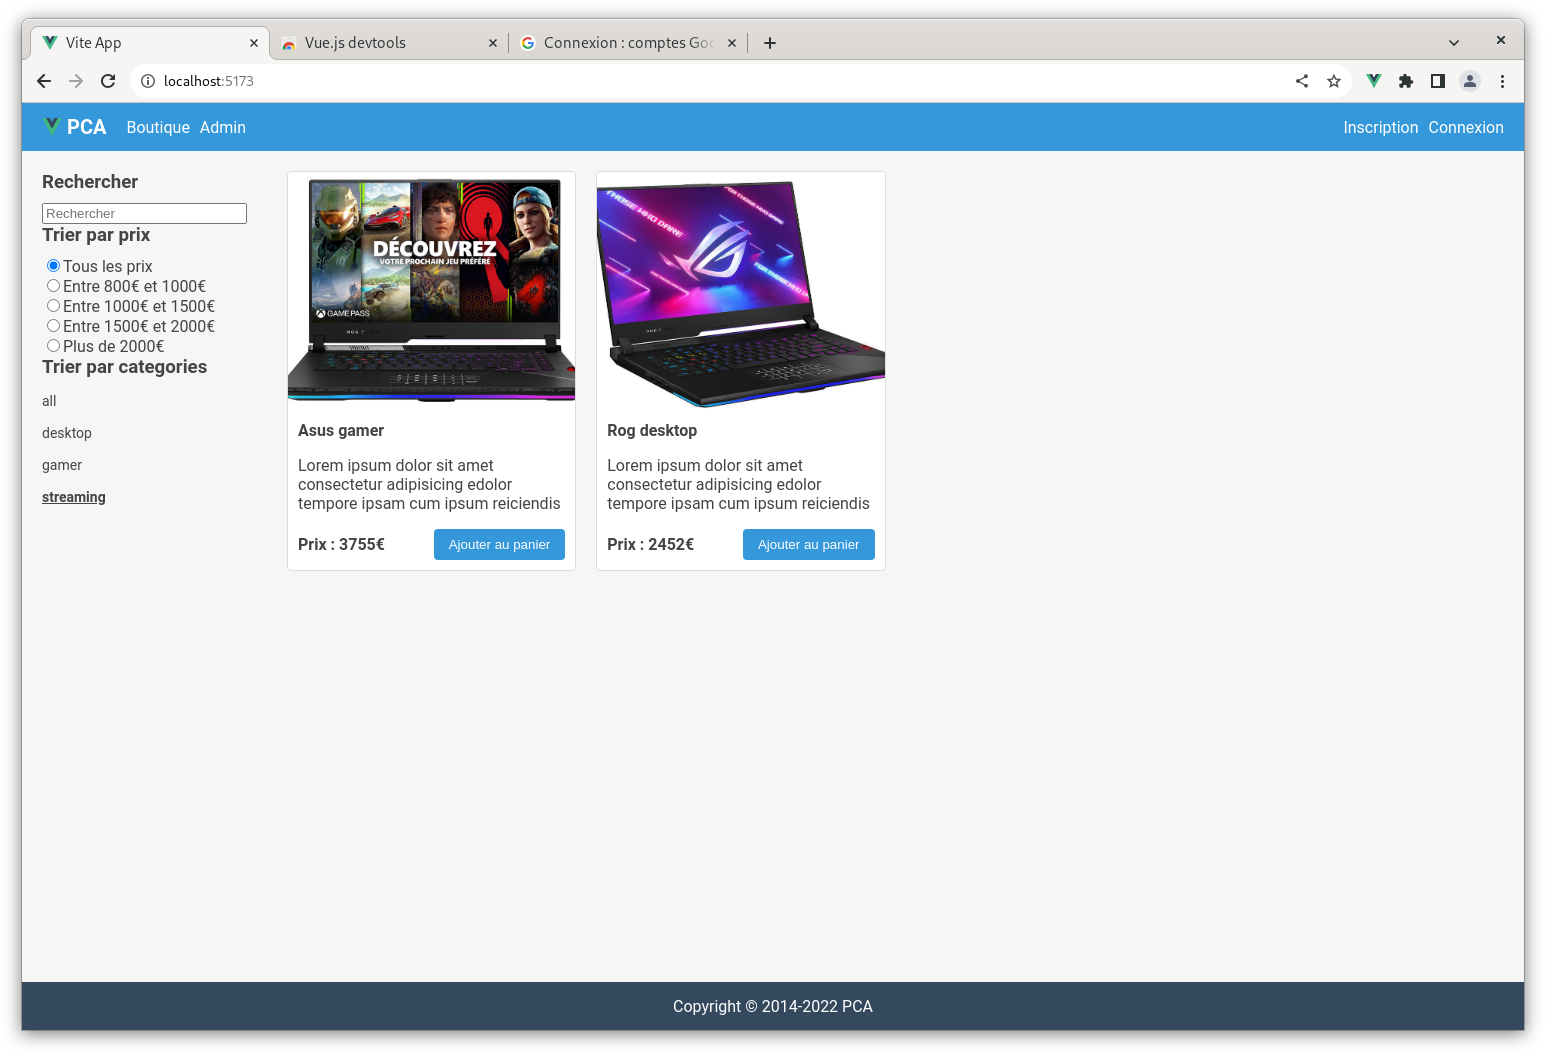
\includegraphics[width=15cm]{images/image27.png}
\end{center}
%%%%%%%%%%%%%%%%%%%%%%%%%%%%%%%%%%%%%%%%%%%%%%%%%%%%%%%%%%%%%%%%%%%%%%%

\section{Reset des filtres}
\subsection{Modification de {\tt ShopFilters.vue}}
Nous ajoutons la reset des filtres et l'affichage du nombre de résultat :
\begin{minted}[
mathescape,
framesep=2mm,
baselinestretch=1.2,
fontsize=\footnotesize,
bgcolor=LightGray,
%linenos
]{html}
<script setup lang="ts">
import type {
  FiltersInterface,
  FilterUpdate,
  Category,
} from '../../interfaces';
defineProps<{
  filters: FiltersInterface;
  nbrOfProducts: number;
}>();
const emit = defineEmits<{
  (e: 'updateFilter', filterUpdate: FilterUpdate): void;
}>();
</script>

<template>
  <div class="p-20 d-flex flex-column">
    <section class="mb-20">
      <h3 class="mb-10">Rechercher</h3>
      <input
        :value="filters.search"
        @input="emit('updateFilter', { search: ($event.target as HTMLInputElement).value })"
        type="text"
        placeholder="Rechercher"
      />
    </section>
    <section class="mb-20">
      <h3 class="mb-10">Trier par prix</h3>
      <div
        class="mb-5"
        v-for="priceRange of ([[0, 10000], [800, 1000], [1000, 1500], [1500, 2000], [2000, 10000]] as [number, number][])"
      >
        <input
          :checked="filters.priceRange[0] === priceRange[0]"
          type="radio"
          @input="emit('updateFilter', { priceRange })"
          name="priceRange"
          :id="priceRange[0] + ''"
        />
        <label :for="priceRange[0] + ''">
          {{
            priceRange[0] === 0
              ? 'Tous les prix'
              : priceRange[0] === 2000
              ? 'Plus de 2000€'
              : `Entre ${priceRange[0]}€ et ${priceRange[1]}€`
          }}
        </label>
      </div>
    </section>
    <section class="mb-20 flex-fill">
      <h3 class="mb-10">Trier par categories</h3>
      <p
        class="category"
        :class="{ selected: filters.category === category }"
        v-for="category in (['all', 'desktop', 'gamer', 'streaming'] as Category[])"
        @click="emit('updateFilter', { category })"
      >
        {{ category }}
      </p>
    </section>
    <small class="mb-5">
      Nombre de résultats:
      <strong>{{ nbrOfProducts }}</strong>
    </small>
    <button class="btn btn-danger" @click="emit('updateFilter', {})">
      Supprimer les filtres
    </button>
  </div>
</template>

<style lang="scss" scoped>
.category {
  font-size: 14px;
  line-height: 18px;
  cursor: pointer;
  &:hover {
    text-decoration: underline;
  }
}
.selected {
  font-weight: bold;
  text-decoration: underline;
}
</style>

\end{minted}

% $
\subsection{Modification de {\tt Shop.vue}}
Il ne faut pas oublier de modifier le composant {\color{monOrange} Shop} pour passer en {\color{monOrange} prop} le nombre de résultats :
\begin{minted}[
mathescape,
framesep=2mm,
baselinestretch=1.2,
fontsize=\footnotesize,
bgcolor=LightGray,
%linenos
]{html}
<script setup lang="ts">
import type {
  FiltersInterface,
  ProductInterface,
  FilterUpdate,
} from '../../interfaces';
import ShopProductList from './ShopProductList.vue';
import ShopFilters from './ShopFilters.vue';

defineProps<{
  products: ProductInterface[];
  filters: FiltersInterface;
}>();

const emit = defineEmits<{
  (e: 'addProductToCart', productId: number): void;
  (e: 'updateFilter', updateFilter: FilterUpdate): void;
}>();
</script>

<template>
  <div class="d-flex flex-row">
    <ShopFilters
      :filters="filters"
      :nbr-of-products="products.length"
      @update-filter="emit('updateFilter', $event)"
      class="shop-filter"
    />
    <ShopProductList
      class="flex-fill"
      @add-product-to-cart="emit('addProductToCart', $event)"
      :products="products"
    />
  </div>
</template>

<style lang="scss" scoped>
.shop-filter {
  flex: 0 0 200px;
}
</style>
\end{minted}
Code de la vidéo
Voici le code de la vidéo :
\begin{center}
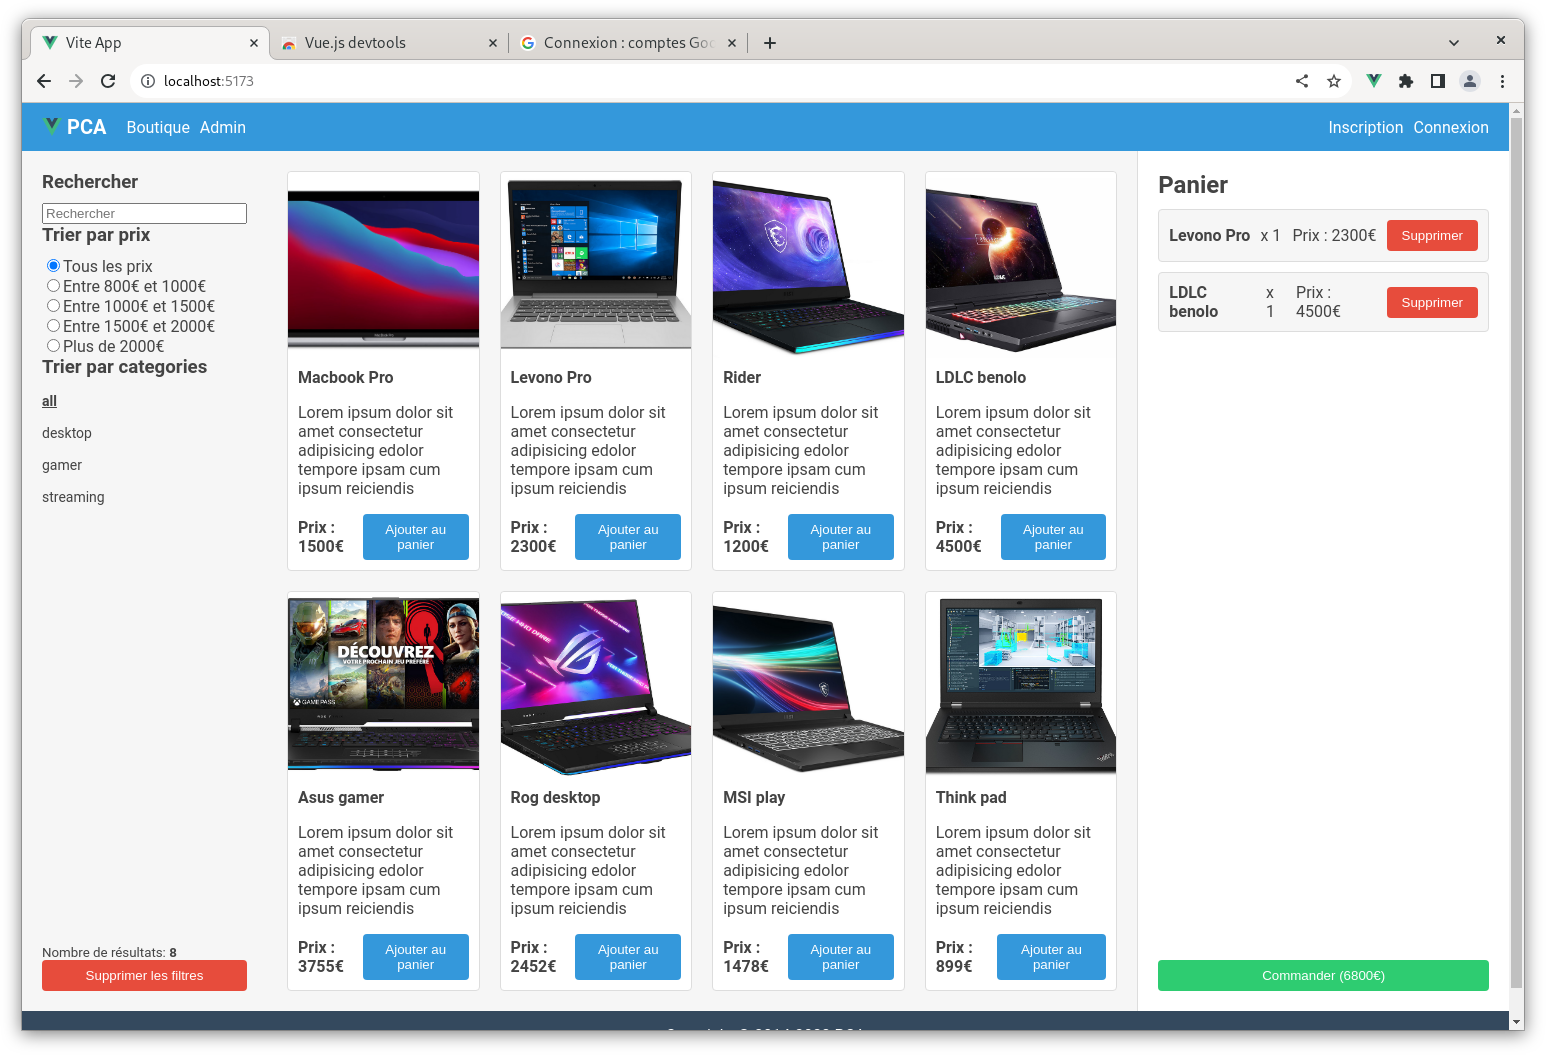
\includegraphics[width=15cm]{images/image28.png}
\end{center}

	\chapter{Les fonctionnalités avancées des composants}
	\section{Introduction au chapitre}
\subsection{Objectifs du chapitre}
Nous allons voir comment utiliser {\color{monOrange}v-model} sur les composants. Nous allons étudier les cascades d'attributs, les {\color{monOrange}slots}, l'injection avec {\color{monOrange}Provide} et {\color{monOrange}Inject}.

Nous verrons également des fonctions utilitaires permettant de transformer des objets réactifs en références. Enfin, nous verrons les composants asynchrones.

\subsection{Code de la vidéo}
Pour rappel, la directive {\color{monOrange}v-model} équivaut à l'utilisation de {\color{monOrange}v-bind} sur l'attribut value et de l'utilisation de {\color{monOrange}v-on} sur l'événement input. Voici l'équivalent de {\color{monOrange}v-model} :


%%%%%%%%%%%%%%%%%%%%%%%%%%%%%%%%%%%%%%%%%%%%%%%%%%%%%%%%%%%%%

\section{Utilisation de la directive v-model sur des composants}
\subsection{Fonctionnement de {\color{monOrange}v-model} avec un composant}
Lorsque vous utilisez {\color{monOrange}v-model} sur un composant enfant :
\begin{minted}[
mathescape,
framesep=2mm,
baselinestretch=1.2,
%fontsize=\footnotesize,
bgcolor=LightGray,
%linenos
]{html}
<Enfant v-model="uneProp" />
\end{minted}
Cela revient en fait exactement à :
\begin{minted}[
mathescape,
framesep=2mm,
baselinestretch=1.2,
fontsize=\footnotesize,
bgcolor=LightGray,
%linenos
]{html}
<Enfant
  :modelValue="uneProp"
  @update:modelValue="val => uneProp = val"
/>
\end{minted}
Cela signifie que dans le composant enfant il faut émettre un événement {\color{monOrange}update:modelValue} et déclarer une {\color{monOrange}prop modelValue} :
\begin{minted}[
mathescape,
framesep=2mm,
baselinestretch=1.2,
fontsize=\footnotesize,
bgcolor=LightGray,
%linenos
]{html}
<script setup>
defineProps<{
  modelValue: string;
}>();
defineEmits<{
  (e: 'update:modelValue', value: string);
}>();
</script>

<template>
  <input
    :value="modelValue"
    @input="$emit('update:modelValue', $event.target.value)"
  />
</template>
\end{minted}
\subsection{Changer le nom de la {\color{monOrange}prop} et de l'événement}
Comme nous venons de le voir, par défaut, la {\color{monOrange}prop} reçue par le composant enfant est {\color{monOrange}modelValue} et l'événement qu'il doit ressentir est {\color{monOrange}update:modelValue}. Il est possible de modifier le nom en passant un argument à {\color{monOrange}v-model} :
\begin{minted}[
mathescape,
framesep=2mm,
baselinestretch=1.2,
fontsize=\footnotesize,
bgcolor=LightGray,
%linenos
]{html}
<Enfant v-model:unNom="uneProp" />
\end{minted}
Vous pouvez ensuite utiliser ce nom dans le composant enfant :
\begin{minted}[
mathescape,
framesep=2mm,
baselinestretch=1.2,
fontsize=\footnotesize,
bgcolor=LightGray,
%linenos
]{html}
<script setup>
defineProps<{
  unNom: string;
}>();
defineEmits<{
  (e: 'update:unNom', value: string);
}>();
</script>

<template>
  <input
    type="text"
    :value="unNom"
    @input="$emit('update:unNom', $event.target.value)"
  />
</template>
\end{minted}
\subsection{Utiliser plusieurs directives {\color{monOrange}v-model}}
Vous pouvez sans problème utiliser plusieurs directives v-model sur un composant :
\begin{minted}[
mathescape,
framesep=2mm,
baselinestretch=1.2,
fontsize=\footnotesize,
bgcolor=LightGray,
%linenos
]{html}
<Enfant v-model:une-prop="uneProp" v-model:une-autre-prop="uneAUtreProp" />
\end{minted}
Par exemple :
\begin{minted}[
mathescape,
framesep=2mm,
baselinestretch=1.2,
fontsize=\footnotesize,
bgcolor=LightGray,
%linenos
]{html}
<Modal v-model:prenom="prenom" v-model:nom="nom" />
\end{minted}
Et nous aurions dans le composant enfant :
\begin{minted}[
mathescape,
framesep=2mm,
baselinestretch=1.2,
fontsize=\footnotesize,
bgcolor=LightGray,
%linenos
]{html}
<template>
  <input
    type="text"
    :value="prenom"
    @input="$emit('update:prenom', $event.target.value)"
  />
  <input
    type="text"
    :value="nom"
    @input="$emit('update:nom', $event.target.value)"
  />
</template>

<script setup lang="ts">
defineProps<{
  prenom: string;
  nom: string;
}>();

defineEmits<{
  (e: 'update:prenom', value: string);
  (e: 'update:nom', value: string);
}>();
</script>

<style scoped lang="scss"></style>
\end{minted}
Voici l'exemple exécutable :


\subsection{Utiliser des modificateurs}
Vous pouvez utiliser des modificateurs personnalisés ou définis par {\color{monOrange}Vue.js}, comme par exemple {\color{monOrange}trim, number} etc. Par exemple, pour supprimer les espaces possibles avant ou après :
\begin{minted}[
mathescape,
framesep=2mm,
baselinestretch=1.2,
fontsize=\footnotesize,
bgcolor=LightGray,
%linenos
]{html}
<Modal v-model:prenom.trim="prenom" v-model:nom.trim="nom" />
\end{minted}
Pour utiliser un modificateur personnalisé, il faut utiliser côté parent :
\begin{minted}[
mathescape,
framesep=2mm,
baselinestretch=1.2,
fontsize=\footnotesize,
bgcolor=LightGray,
%linenos
]{html}
<Modal v-model:prenom="prenom" v-model:nom.exemple="nom" />
\end{minted}
Et côté enfant :
\begin{minted}[
mathescape,
framesep=2mm,
baselinestretch=1.2,
fontsize=\footnotesize,
bgcolor=LightGray,
%linenos
]{html}
<template>
  <input
    type="text"
    :value="prenom"
    @input="$emit('update:prenom', $event.target.value)"
  />
  <input
    type="text"
    :value="nom"
    @input="emitName"
  />
</template>

<script setup lang="ts">
defineProps<{
  prenom: string;
  nom: string;
  nameModifiers?: { [s: string]: boolean };
}>();

defineEmits<{
  (e: 'update:prenom', value: string);
  (e: 'update:nom', value: string);
}>();

function emitName(event) {
  let value = (event.target as HTMLInputElement).value;
  if (props.modelModifiers.exemple) {
    // Modifier la valeur comme on souhaite si le modificateur est présent :
    value = value.toUpperCase();
  }
  emit('update:modelValue', value);
}
</script>

<style scoped lang="scss"></style>
\end{minted}
\subsection{Code de la vidéo}
Pour rappel, la directive {\color{monOrange}v-model} équivaut à l'utilisation de {\color{monOrange}v-bind} sur l'attribut value et de l'utilisation de {\color{monOrange}v-on} sur l'événement {\color{monOrange}input}. Voici l'équivalent de {\color{monOrange}v-model} :

%%%%%%%%%%%%%%%%%%%%%%%%%%%%%%%%%%%%%%%%%%%%%%%%%%%%%%%%%%%%%%%


\section{Cascade d'attributs}
\subsection{Les attributs en cascade}
{\em Les attributs en cascade sont rarement utilisés, vous pouvez passer rapidement pour une première approche de {\color{monOrange}Vue.js} et y revenir plus tard.}

Un attribut en cascade est un attribut ou un écouteur d'événement déclaré avec {\color{monOrange}v-on} qui est passé à un composant sans être déclaré précisé, c'est-à- dire sans utiliser de {\color{monOrange}props}. Par exemple, si nous avons le composant enfant :
\begin{minted}[
mathescape,
framesep=2mm,
baselinestretch=1.2,
fontsize=\footnotesize,
bgcolor=LightGray,
%linenos
]{html}
<template>
  <h1>Hello</h1>
</template>
\end{minted}
Et que nous déclarons un attribut sur celui-ci dans le composant parent :
\begin{minted}[
mathescape,
framesep=2mm,
baselinestretch=1.2,
fontsize=\footnotesize,
bgcolor=LightGray,
%linenos
]{html}
<template>
  <Enfant class="large" />
</template>
\end{minted}
Le composant enfant rendu sur le DOM sera :
\begin{minted}[
mathescape,
framesep=2mm,
baselinestretch=1.2,
fontsize=\footnotesize,
bgcolor=LightGray,
%linenos
]{html}
<h1 class="large">Hello</h1>
\end{minted}
\subsection{Fusionnement d'attributs}
Comme vu précédemment, si le composant enfant a déjà un attribut déclaré, les valeurs seront fusionnées. En reprenant l'exemple avec l'attribut {\color{monOrange}class} :
\begin{minted}[
mathescape,
framesep=2mm,
baselinestretch=1.2,
fontsize=\footnotesize,
bgcolor=LightGray,
%linenos
]{html}
<template>
  <h1 class="titre">Hello</h1>
</template>
\end{minted}
Et dans le composant parent :
\begin{minted}[
mathescape,
framesep=2mm,
baselinestretch=1.2,
fontsize=\footnotesize,
bgcolor=LightGray,
%linenos
]{html}
<template>
  <Enfant class="large" />
</template>
\end{minted}
Nous aurons :
\begin{minted}[
mathescape,
framesep=2mm,
baselinestretch=1.2,
fontsize=\footnotesize,
bgcolor=LightGray,
%linenos
]{html}
<h1 class="titre large">Hello</h1>
\end{minted}
\subsection{Ecouteurs déclarés avec {\color{monOrange}v-on}}
C'est exactement le même principe avec les écouteurs d'événements déclarés en utilisant {\color{monOrange}v-on}. Si le {\color{monOrange}template} du composant parent est :
\begin{minted}[
mathescape,
framesep=2mm,
baselinestretch=1.2,
fontsize=\footnotesize,
bgcolor=LightGray,
%linenos
]{html}
<template>
  <Enfant @click="onClick" />
</template>
<script>
function onClick() {
  console.log("clic");
}
</script>
\end{minted}
L'écouteur sera placé automatiquement sur l'élément racine du composant enfant. Un clic sur le composant enfant déclenchera donc le gestionnaire déclaré dans le composant parent. A noter que si l'élément racine du composant enfant a déjà un ou plusieurs gestionnaires d'événements déclarés, ils seront également exécutés. Cela ne les remplacera pas.

\subsection{Utilisation de {\color{monOrange}\$attrs} côté {\color{monOrange}template}}
{\color{monOrange}Vue} met à disposition automatiquement une propriété {\color{monOrange}\$attrs} que vous pouvez utiliser dans le {\color{monOrange}template} du composant enfant. Elle contient tous les attributs et les écouteurs d'événements passés en cascade. C'est par exemple utile si le composant enfant n'a pas d'élément racine, pour décider de placer les attributs reçus sur un élément particulier :
\begin{minted}[
mathescape,
framesep=2mm,
baselinestretch=1.2,
fontsize=\footnotesize,
bgcolor=LightGray,
%linenos
]{html}
<template>
  <h1>Hello</h1>
  <h2 v-bind="$attrs">Hello 2</h2>
</template>
\end{minted}
\subsection{Utilisation de {\color{monOrange}useAttrs()} côté {\color{monOrange}script}}
Il est également possible d'accéder aux attributs en utilisant {\color{monOrange}useAttrs()} cîoté {\color{monOrange}script} :
\begin{minted}[
mathescape,
framesep=2mm,
baselinestretch=1.2,
fontsize=\footnotesize,
bgcolor=LightGray,
%linenos
]{html}
<script setup>
  
import { useAttrs } from 'vue';

const attrs = useAttrs();
</script>
\end{minted}
\subsection{Désactivation du passage automatique des attributs}
Il est possible de désactiver le passage automatique des attributs dans le cas où par exemple, vous avez bien un élément racine sur le composant enfant mais que vous souhaitez appliquer les attributs sur d'autres éléments :
\begin{minted}[
mathescape,
framesep=2mm,
baselinestretch=1.2,
fontsize=\footnotesize,
bgcolor=LightGray,
%linenos
]{html}
<template>
  <div class="uneClasse">
    <h1>Hello</h1>
    <h2 v-bind="$attrs">Hello 2</h2>
  </div>
</template>

<script lang="ts">
export default {
  inheritAttrs: false,
};
</script>

<script setup lang="ts"></script>
\end{minted}
Notez bien l'utilisation de deux balises {\color{monOrange}scripts} ! Elles seront fusionnées automatiquement avec la configuration par {\color{monOrange}Vite}.

\subsection{Code de la vidéo}
Voici le code de la vidéo :

%%%%%%%%%%%%%%%%%%%%%%%%%%%%%%%%%%%%%%%%%%%%%%%%%%%%%%%%%%%%%

\section{Présentation des slots}
\subsection{Les {\color{monOrange}slots}}
Les {\color{monOrange}slots} permettent de passer des parties de {\color{monOrange}template} d'un composant parent à un composant enfant. Nous avions vu les {\color{monOrange}props} qui permettent de passer des valeurs JavaScript d'un composant parent à un composant enfant.

Les {\color{monOrange}slots} permettent de passer du HTML. Pour utiliser les {\color{monOrange}slots}, il faut utiliser le composant enfant avec deux balises et mettre le fragment HTML à passer, c'est-à -dire le {\color{monOrange}slot}, entre ces deux balises :
\begin{minted}[
mathescape,
framesep=2mm,
baselinestretch=1.2,
fontsize=\footnotesize,
bgcolor=LightGray,
%linenos
]{html}
<Enfant>
  J’insère du contenu ici pour le passer au composant enfant.
</Enfant>
\end{minted}
Dans le composant enfant, il faut utiliser une balise {\color{monOrange}<slot>} pour indiquer où afficher le contenu passé :
\begin{minted}[
mathescape,
framesep=2mm,
baselinestretch=1.2,
fontsize=\footnotesize,
bgcolor=LightGray,
%linenos
]{html}
<template>
  // Le contenu sera projeté à la place de slot :
  <slot></slot>
</template>
\end{minted}
Voici le schéma officiel pour les {\color{monOrange}slots} avec un autre exemple simple :
\begin{center}
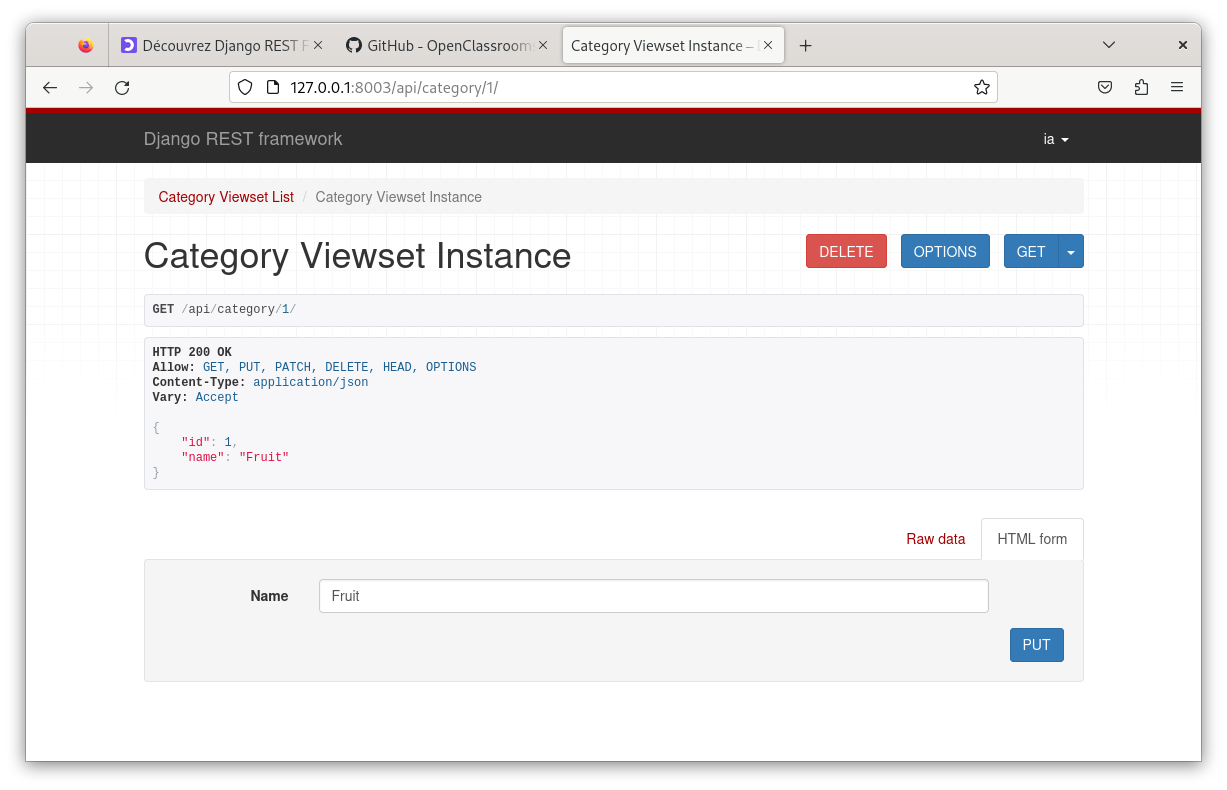
\includegraphics[width=10cm]{images/image10.png}
\end{center}

Dans le {\color{monOrange}template} du parent nous déclarons le fragment HTML à passer : en l'occurrence simplement le texte {\color{monOrange}Click Me}. Nous déclarons le contenu entre les balises du composant enfant {\color{monOrange}FancyButton}.

Dans le composant enfant, nous utilisons les balises {\tt <slot>} pour indiquer où insérer le contenu passé, dans l'occurrence le texte {\color{monOrange}Click Me}. Le rendu final sur le DOM sera donc :
\begin{minted}[
mathescape,
framesep=2mm,
baselinestretch=1.2,
fontsize=\footnotesize,
bgcolor=LightGray,
%linenos
]{html}
<button>
  Click Me
</button>
\end{minted}
Il est possible de passer n'importe quel contenu HTML comme par exemple une {\color{monOrange}div} :
\begin{minted}[
mathescape,
framesep=2mm,
baselinestretch=1.2,
fontsize=\footnotesize,
bgcolor=LightGray,
%linenos
]{html}
<template>
  <Enfant>
    <div>
      J’insère du contenu ici pour le passer au composant enfant.
    </div>
  </Enfant>
</template>
\end{minted}
Il est même possible de passer un autre composant :
\begin{minted}[
mathescape,
framesep=2mm,
baselinestretch=1.2,
fontsize=\footnotesize,
bgcolor=LightGray,
%linenos
]{html}
<template>
  <Enfant>
    <AutreComposant></AutreComposant>
  </Enfant>
</template>
\end{minted}
Le composant sera également remplacé à l'endroit de {\color{monOrange}slot}.

\subsection{Portée des variables}
Le contenu déclaré dans le composant parent a accès aux propriétés du composant parent :
\begin{minted}[
mathescape,
framesep=2mm,
baselinestretch=1.2,
fontsize=\footnotesize,
bgcolor=LightGray,
%linenos
]{html}
<template>
  <span>{{ message }}</span>
  <Enfant>{{ message }}</Enfant>
</template>
\end{minted}
Ici si le composant parent a une propriété {\color{monOrange}message} côté {\color{monOrange}script}, aucun problème pour l'utiliser dans le contenu à passer en {\color{monOrange}slot} au composant enfant.

En revanche, le contenu n'a pas accès par défaut aux propriétés du composant enfant. Donc dans notre exemple, si la propriété {\color{monOrange}message} était déclarée dans le composant enfant, nous aurions une erreur.

\subsection{Les {\color{monOrange}slots} nommés}
Il est parfois nécessaire de projeter plusieurs contenus à des endroits précis. Dans ce cas, il faut utiliser plusieurs éléments {\color{monOrange}slot} et les identifiants de manière unique. Pour nommer un {\color{monOrange}slot} côté composant parent, il suffit d'utiliser la directive {\color{monOrange}v-slot} sur l'élément projeté et de lui passer l'identifiant :
\begin{minted}[
mathescape,
framesep=2mm,
baselinestretch=1.2,
fontsize=\footnotesize,
bgcolor=LightGray,
%linenos
]{html}
<template>
  <Enfant>
    <h1 v-slot:header>Titre de mon site</h1>
    <p v-slot:footer>Qui sommes-nous ?</p>
  </Enfant>
</template>
\end{minted}
La notation raccourcie de la directive {\color{monOrange}v-slot} est {\color{monOrange}\#}, nous pouvons donc faire :
\begin{minted}[
mathescape,
framesep=2mm,
baselinestretch=1.2,
fontsize=\footnotesize,
bgcolor=LightGray,
%linenos
]{html}
<template>
  <Enfant>
    <h1 #header>Titre de mon site</h1>
    <p v-#footer>Qui sommes-nous ?</p>
  </Enfant>
</template>
\end{minted}
Dans notre exemple nous avons défini deux {\color{monOrange}slot header} et {\color{monOrange}footer} qui nous permettent de référencer les contenus à projeter. Dans le composant enfant, il suffit d'utiliser l'attribut {\color{monOrange}name} sur un {\color{monOrange}slot} pour indiquer que le contenu référencé doit être projeté à cet endroit :
\begin{minted}[
mathescape,
framesep=2mm,
baselinestretch=1.2,
fontsize=\footnotesize,
bgcolor=LightGray,
%linenos
]{html}
<template>
  <header>
    <slot name="header"></slot>
  </header>
  <footer>
    <slot name="footer"></slot>
  </footer>
<template>
\end{minted}
Il est également possible de créer des identifiants dynamiques pour les {\color{monOrange}slots} dans les composants parents :
\begin{minted}[
mathescape,
framesep=2mm,
baselinestretch=1.2,
fontsize=\footnotesize,
bgcolor=LightGray,
%linenos
]{html}
<template v-slot:[nomDynamique]>
    Du contenu HTML
</template>
\end{minted}
Vous pouvez également utiliser la notation raccourcie :
\begin{minted}[
mathescape,
framesep=2mm,
baselinestretch=1.2,
fontsize=\footnotesize,
bgcolor=LightGray,
%linenos
]{html}
<template #[nomDynamique]>
  Du contenu HTML
</template>
\end{minted}
\subsection{Contenu par défaut}
Il est également possible de définir un contenu par défaut si aucun contenu n'est passé.

Il suffit de mettre du contenu par défaut entre les balises {\tt <slot>} dans le composant enfant pour que celui-ci soit considéré comme contenu par défaut :
\begin{minted}[
mathescape,
framesep=2mm,
baselinestretch=1.2,
fontsize=\footnotesize,
bgcolor=LightGray,
%linenos
]{html}
<template>
  <slot name="header">Mon titre par défaut si aucun contenu n’est passé</slot>
<template>
\end{minted}
\subsection{Code de la vidéo}
Voici le code de la vidéo :

%%%%%%%%%%%%%%%%%%%%%%%%%%%%%%%%%%%%%%%%%%%%%%%%%%%%%%%%%%%%%%

\section{Portes des machines à sous}
\subsection{Passer des données aux slots}
Nous avons vu que par défaut, le contenu des {\color{monOrange}slots} ne peut accéder aux propriétés déclarées dans le composant enfant.

Il est cependant possible de passer des valeurs aux contenus des {\color{monOrange}slots} depuis le composant enfant. Pour ce faire, il faut passer des attributs aux {\color{monOrange}slots}, exactement de la même manière que pour les {\color{monOrange}props} aux composants. Bien sûr, cette fois-ci nous sommes dans le composant enfant :
\begin{minted}[
mathescape,
framesep=2mm,
baselinestretch=1.2,
fontsize=\footnotesize,
bgcolor=LightGray,
%linenos
]{html}
<div>
  <slot :prop="uneValeur" :autreProp="42"></slot>
</div>
\end{minted}
Dans le composant parent, nous pouvons utiliser ces propriétés passées depuis le composant enfant dans les contenus :
\begin{minted}[
mathescape,
framesep=2mm,
baselinestretch=1.2,
fontsize=\footnotesize,
bgcolor=LightGray,
%linenos
]{html}
<Enfant v-slot="slotProps">
  {{ slotProps.prop }} {{ slotProps.autreProp }}
</Enfant>
\end{minted}
Cela fonctionne également avec les {\color{monOrange}slots} nommés :
\begin{minted}[
mathescape,
framesep=2mm,
baselinestretch=1.2,
fontsize=\footnotesize,
bgcolor=LightGray,
%linenos
]{html}
<Enfant>
  <template #header="headerProps">
    {{ headerProps }}
  </template>

  <template #default="defaultProps">
    {{ defaultProps }}
  </template>

  <template #footer="footerProps">
    {{ footerProps }}
  </template>
</Enfant>
\end{minted}
Dans le composant enfant :
\begin{minted}[
mathescape,
framesep=2mm,
baselinestretch=1.2,
fontsize=\footnotesize,
bgcolor=LightGray,
%linenos
]{html}
<slot name="header" :uneProp="uneValeur"></slot>

<slot name="footer" :uneProp2="autreVal"></slot>
\end{minted}
\subsection{Code de la vidéo}
Voici le code de la vidéo :

%%%%%%%%%%%%%%%%%%%%%%%%%%%%%%%%%%%%%%%%%%%%%%%%%%%%%%%%%%%%%%

\section{Provide et Inject}
\subsection{Passer des données à travers plusieurs composants}
Supposons que vous vouliez passer des données à des composants enfants éloignés dans l'arbre. Vous pouvez utiliser des {\color{monOrange}props} sur plusieurs niveaux :
\begin{center}
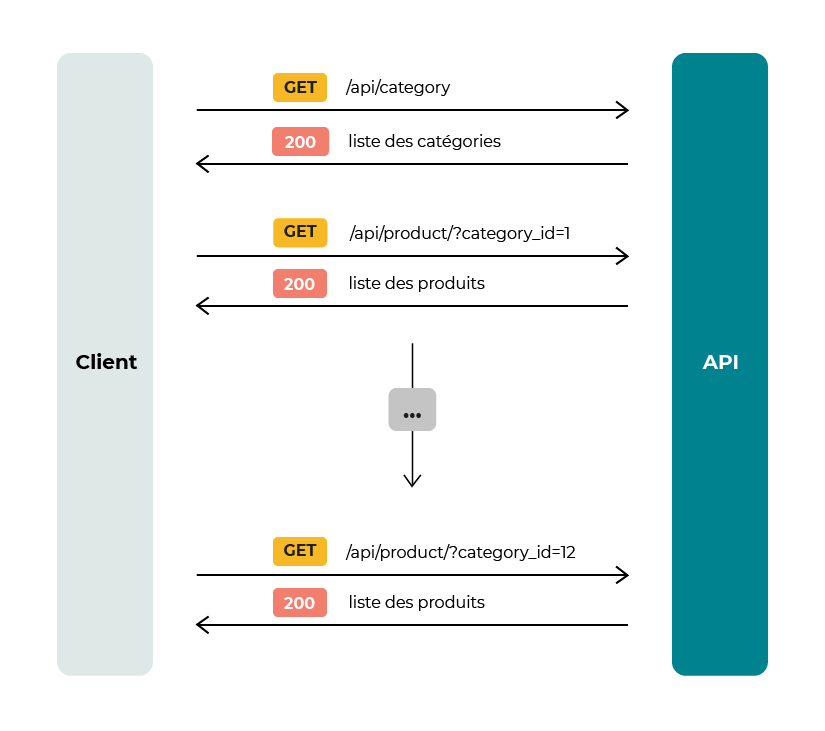
\includegraphics[width=10cm]{images/image11.png}
\end{center}

C'est d'ailleurs ce que nous avons fait dans le projet. Mais supposons que les composants ciblés soient à 3 ou 4 voir plus niveaux du composant contenant les données et que les composants intermédiaires n'étaient pas besoin de ces données. Comment faire pour passer des données sans devoir déclarer les mêmes {\color{monOrange}props} dans tous les composants ancêtres des composants cibles ? C'est là qu'interviennent {\color{monOrange}provide} et {\color{monOrange}inject} :
\begin{center}
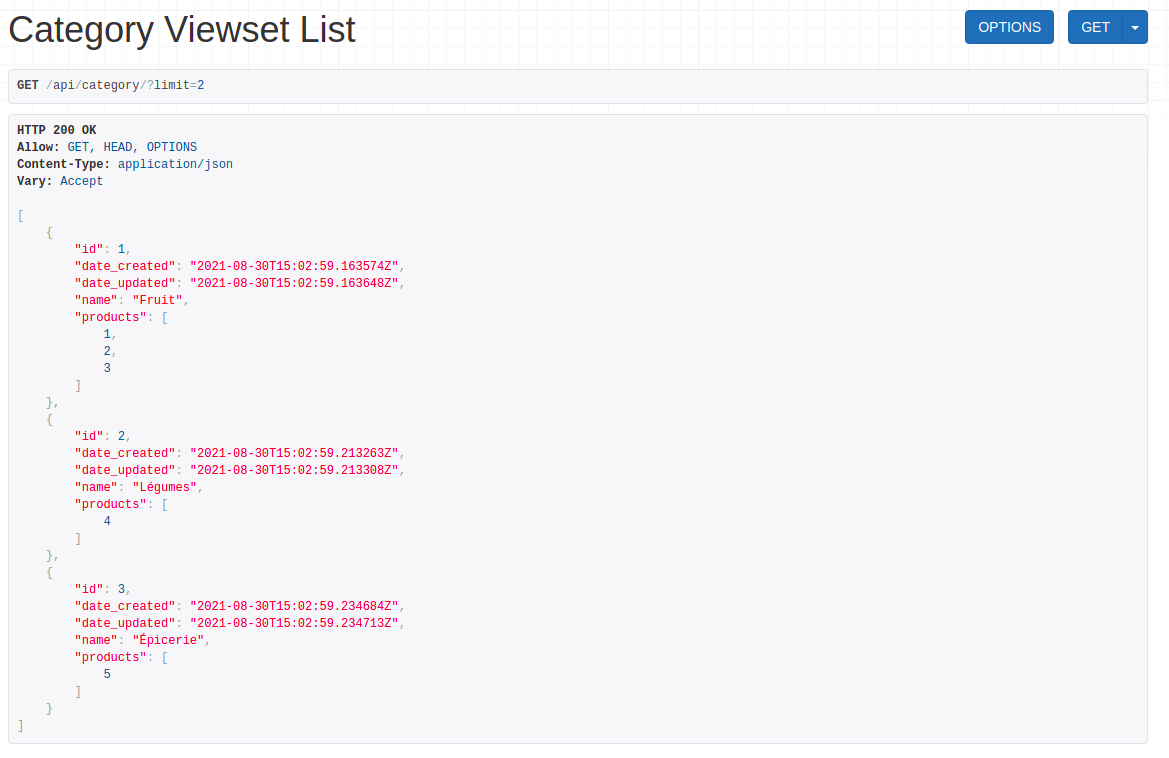
\includegraphics[width=10cm]{images/image12.png}
\end{center}

\subsection{La fonction {\color{monOrange}provide()}}
La fonction {\color{monOrange}provide()} permet de mettre à disposition des données réactives ou non à tous les composants descendants du composant l'utilisant. La syntaxe est :
\begin{minted}[
mathescape,
framesep=2mm,
baselinestretch=1.2,
fontsize=\footnotesize,
bgcolor=LightGray,
%linenos
]{html}
<script setup>
import { provide } from 'vue';

provide('clé', valeur);
</script>
\end{minted}
La clé d'injection doit être une chaîne de caractères mais la valeur peut être une valeur en dur ou une propriété réactive :
\begin{minted}[
mathescape,
framesep=2mm,
baselinestretch=1.2,
fontsize=\footnotesize,
bgcolor=LightGray,
%linenos
]{javascript}
import { ref, provide } from 'vue';

const compteur = ref(0);
provide('compteur', compteur);
\end{minted}
\subsection{Fournir des valeurs globalement}
Pour fournir des données à toute l'application et non seulement aux composants descendants d'un composant, vous pouvez utiliser la méthode provide() sur app dans main.ts :
\begin{minted}[
mathescape,
framesep=2mm,
baselinestretch=1.2,
fontsize=\footnotesize,
bgcolor=LightGray,
%linenos
]{html}
import { createApp } from 'vue';
import App from './App.vue';

const app = createApp(App);

app.provide('API_URL', 'https://restapi.fr/api');

app.mount('#app');
\end{minted}
\subsection{Injecter les données avec la fonction {\color{monOrange}inject()}}
La fonction {\color{monOrange}inject()} permet de récupérer les données fournies par {\color{monOrange}provide} dans un composant descendant :
\begin{minted}[
mathescape,
framesep=2mm,
baselinestretch=1.2,
fontsize=\footnotesize,
bgcolor=LightGray,
%linenos
]{html}
<script setup>
import { inject } from 'vue';

const compteur = inject('compteur');
</script>
\end{minted}
Comme nous utilisons {\color{monOrange}TypeScript}, il faut taper la valeur reçue en utilisant un type générique :
\begin{minted}[
mathescape,
framesep=2mm,
baselinestretch=1.2,
fontsize=\footnotesize,
bgcolor=LightGray,
%linenos
]{html}
const compteur = inject<number>('compteur');
\end{minted}
En effet, sans ça {\color{monOrange}TypeScript} n'a aucun moyen de savoir le type de la valeur retournée par la fonction {\color{monOrange}inject()}.

Lorsque vous êtes certain que la valeur fournie par {\color{monOrange}provide()} sera présente, et qu'elle ne peut donc pas être undefined, vous pouvez l'indiquer à {\color{monOrange}TypeScript} en utilisant ! :
\begin{minted}[
mathescape,
framesep=2mm,
baselinestretch=1.2,
fontsize=\footnotesize,
bgcolor=LightGray,
%linenos
]{html}
const compteur = inject<number>('compteur')!;
\end{minted}
\subsection{Modification des propriétés réactives}
Lorsque vous utilisez {\color{monOrange}provide/inject}, il est recommandé de laisser toutes les modifications des propriétés réactives dans le composant qui utilise {\color{monOrange}provide()}. Autrement dit, retenez la règle qu'il est interdit de modifier une propriété réactive fournie par {\color{monOrange}provide()} dans un composant descendant et qu'il faut le faire dans le composant parent.

{\color{monOrange}Vue.js} met à disposition la fonction {\color{monOrange}readonly()} pour ne pas oublier de respecter cette règle. Si vous voulez modifier des propriétés réactives depuis un composant enfant il faut passer une fonction avec {\color{monOrange}provide} qui sera appelée par le composant enfant :
\begin{minted}[
mathescape,
framesep=2mm,
baselinestretch=1.2,
fontsize=\footnotesize,
bgcolor=LightGray,
%linenos
]{html}
<script setup>
import { provide, ref, readonly } from 'vue';

const ville = ref('Paris');

function majVille() {
  ville.value = 'Nice';
}

provide('ville', readonly({
  ville,
  majVille
}));
</script>
\end{minted}
Et dans le composant descendant :
\begin{minted}[
mathescape,
framesep=2mm,
baselinestretch=1.2,
fontsize=\footnotesize,
bgcolor=LightGray,
%linenos
]{html}
<script setup>
import { inject } from 'vue';

const { ville, majVille } = inject<{ ville: string; majVille: () => void }>('ville');
</script>

<template>
  <button @click="majVille">{{ ville }}</button>
</template>
\end{minted}
\subsection{Code de la vidéo}
Voici le code de la vidéo :

	\chapter{HTTP}
	\section{Introduction et requête AJAX}
\subsection{Rappels sur {\color{monOrange}AJAX}}
L'{\color{monOrange}AJAX} est une pratique de permettant de mettre à jour simplement des parties du DOM d'une page HTML au lieu de devoir recharger la page entière.

AJAX permet également d'exécuter du code de manière asynchrone, c'est-à-dire que votre code continue à s'exécuter pendant qu'une ou plusieurs requêtes sont en cours.

{\em N'hésitez pas à revoir le chapitre réseau de la formation JavaScript si tout cela n'est pas parfaitement clair pour vous.}

\subsection{Rappels sur fetch}
{\color{monOrange}fetch} est une {\color{monOrange}Web API} disponible dans tous les navigateurs qui permet d'envoyer des requêtes {\color{monOrange}HTTP}. La syntaxe de l'{\color{monOrange}API} est très simple :
\begin{minted}[
mathescape,
framesep=2mm,
baselinestretch=1.2,
%fontsize=\footnotesize,
bgcolor=LightGray,
%linenos
]{javascript}
const promesse = fetch(url, [options]);
\end{minted}
\begin{enumerate}
\item Le premier paramètre est l'URL cible de la requête.
\item Le second paramètre est un objet d'options que nous étudierons en détails.
\item La Web API retourne une promesse qui sera tenue si le serveur répond.
\item La promesse est résolue avec un objet Response.
\end{enumerate}
A ce stade, vous pouvez accéder aux propriétés suivantes :
\begin{itemize}
\item {\color{monOrange}url :} url de la requête.
\item {\color{monOrange}redirected :} booléen indiquant si la requête a été redirigée par le serveur.
\item {\color{monOrange}status :} code du statut de la requête.
\item {\color{monOrange}ok :} booléen pour savoir si la requête s'est bien déroulée (true si le code du statut est compris entre 200 et 299).
\item {\color{monOrange}type :} type de la requête cors ou basic (nous y reviendrons).
\item {\color{monOrange}statusText :} message du statut de la requête.
\item {\color{monOrange}headers :} headers de la réponse. Il faut utiliser la méthode get() et passer le nom du header à récupérer.
\end{itemize}
\subsection{Le service Dyma restapi.fr}
Nous allons utiliser un service de Dyma pour le backend qui permet notamment de sauvegarder des données facilement en utilisant un véritable service REST.

Ce service est {\color{monOrange}www.restapi.fr} et il permet de sauvegarder et de manipuler des données facilement. Il permet également de générer des données suivant un modèle que vous définissez.

%%%%%%%%%%%%%%%%%%%%%%%%%%%%%%%%%%%%%%%%%%%%%%%%%%%%%%%%%%%%%%%%%%
\section{Requêtes POST}
\subsection{Effectuer une requête POST avec fetch}
Pour effectuer une requête de type POST il faut utiliser deux arguments. Voici un exemple de requête :
\begin{minted}[
mathescape,
framesep=2mm,
baselinestretch=1.2,
fontsize=\footnotesize,
bgcolor=LightGray,
%linenos
]{javascript}
const utilisateur = {
  name: "Paul Dupont"
};
const reponse = await fetch("https:/restapi.fr/users", {
  method: "POST",
  headers: {
    "Content-Type": "application/json"
  },
  body: JSON.stringify(utilisateur)
});
\end{minted}
Nous devons préciser dans l'objet options les propriétés suivantes :
\begin{itemize}
\item {\color{monOrange}method } : La méthode de la requête, par exemple {\tt  DELETE} ou {\tt  POST}.
\item {\color{monOrange}headers} : Les entêtes à ajouter à la requête. Il faut préciser nécessairement le type des données envoyées. Ici nous envoyons des données au format JSON nous spécifions donc {\tt  "Content-Type": "application/json"}.
\item {\color{monOrange}body }: Le contenu de la requête {\tt  POST}. Il doit être au format que nous précisons dans l'entête {\tt  Content-Type}, donc en JSON. Nous devons donc utiliser la méthode {\tt  JSON.stringify()} pour transformer notre objet JavaScript en {\tt  JSON}.

\end{itemize}
\subsection{Code de la vidéo}
Voici le code de la vidéo :
\begin{minted}[
mathescape,
framesep=2mm,
baselinestretch=1.2,
fontsize=\footnotesize,
bgcolor=LightGray,
%linenos
]{html}
<template>
  <div class="container">
    <div class="p-20">
      <h3 class="mb-10">Formulaire</h3>
      <form @submit="mySubmit">
        <input
          v-model="nameValue"
          class="mr-10"
          type="text"
          placeholder="Prénom"
        />
        <input
          v-model="emailValue"
          class="mr-10"
          type="text"
          placeholder="Email"
        />
        <button class="btn btn-primary">Sauvegarder</button>
      </form>
    </div>
    <div class="p-20">
      <h3>Liste des utilisateurs</h3>
      <ul>
        <li v-for="user in state.users">
          <p>{{ user.name }} - {{ user.email }}</p>
        </li>
      </ul>
    </div>
  </div>
</template>

<script setup lang="ts">
import { useForm, useField } from 'vee-validate';
import { reactive } from 'vue';

interface User {
  name: string;
  email: string;
  createdAt?: string;
  _id?: string;
}

const state = reactive<{ users: User[] }>({
  users: [],
});

const { handleSubmit, resetForm } = useForm();

const mySubmit = handleSubmit(async (value) => {
  try {
    const response = await fetch('https://restapi.fr/api/vueuser', {
      method: 'POST',
      body: JSON.stringify(value),
      headers: {
        'Content-Type': 'application/json',
      },
    });
    const user: User = await response.json();
    state.users.push(user);
    resetForm();
  } catch (err) {
    console.error(err);
  }
});

const { value: emailValue } = useField('email');
const { value: nameValue } = useField('name');
</script>

<style lang="scss">
@import './assets/scss/base.scss';
</style>
\end{minted}

%%%%%%%%%%%%%%%%%%%%%%%%%%%%%%%%%%%%%%%%%%%%%%%%%%%%%%%%%%%%%%%%%%%%%%%

\section{Requêtes GET et DELETE}
\subsection{Envoyer une requête {\color{monOrange}GET}}
Sans passer d'option, {\color{monOrange}fetch} va effectuer une requête HTTP avec la méthode {\tt GET} :
\begin{minted}[
mathescape,
framesep=2mm,
baselinestretch=1.2,
fontsize=\footnotesize,
bgcolor=LightGray,
%linenos
]{javascript}
const reponse = await fetch("https://restapi.fr/users");
\end{minted}
Pour lire le contenu de la réponse, il faut la parser, c'est-à-dire attendre que tout le body soit reçu et le lire dans un format particulier. Dans une application, le plus courant sera de parser la réponse au format {\tt JSON} avec la méthode {\tt json()} :
\begin{minted}[
mathescape,
framesep=2mm,
baselinestretch=1.2,
fontsize=\footnotesize,
bgcolor=LightGray,
%linenos
]{javascript}
const reponse = await fetch("https://jsonplaceholder.typicode.com/users");
const donnees = await reponse.json();
\end{minted}
\subsection{Envoyer une requête DELETE}
Pour envoyer une requête HTTP de type {\tt DELETE}, il suffit de préciser cette méthode dans l'objet d'options passé à {\tt fetch()} :
\begin{minted}[
mathescape,
framesep=2mm,
baselinestretch=1.2,
fontsize=\footnotesize,
bgcolor=LightGray,
%linenos
]{javascript}
await fetch(`https://restapi.fr/api/users?id=${userId}`, {
  method: 'DELETE',
});
\end{minted} 

%$
\subsection{Code de la vidéo}
Voici le code de la vidéo :
\begin{minted}[
mathescape,
framesep=2mm,
baselinestretch=1.2,
fontsize=\footnotesize,
bgcolor=LightGray,
%linenos
]{html}
<template>
  <div class="container">
    <div class="p-20">
      <h3 class="mb-10">Formulaire</h3>
      <form @submit="mySubmit">
        <input
          v-model="nameValue"
          class="mr-10"
          type="text"
          placeholder="Prénom"
        />
        <input
          v-model="emailValue"
          class="mr-10"
          type="text"
          placeholder="Email"
        />
        <button class="btn btn-primary">Sauvegarder</button>
      </form>
    </div>
    <div class="p-20">
      <h3>Liste des utilisateurs</h3>
      <ul>
        <li v-for="user in state.users">
          <p class="mr-10">{{ user.name }} - {{ user.email }}</p>
          <button
            @click="deleteUser(user._id)"
            type="button"
            class="btn btn-danger"
          >
            Supprimer
          </button>
        </li>
      </ul>
    </div>
  </div>
</template>

<script setup lang="ts">
import { useForm, useField } from 'vee-validate';
import { reactive } from 'vue';

interface User {
  name: string;
  email: string;
  createdAt?: string;
  _id?: string;
}

const state = reactive<{ users: User[] }>({
  users: [],
});

const { handleSubmit, resetForm } = useForm();

const mySubmit = handleSubmit(async (value) => {
  try {
    const response = await fetch('https://restapi.fr/api/vueusers', {
      method: 'POST',
      body: JSON.stringify(value),
      headers: {
        'Content-Type': 'application/json',
      },
    });
    const user: User = await response.json();
    state.users.push(user);
    resetForm();
  } catch (err) {
    console.error(err);
  }
});

const { value: emailValue } = useField('email');
const { value: nameValue } = useField('name');

async function fetchUsers() {
  try {
    const response = await fetch('https://restapi.fr/api/vueusers');
    const users: User | User[] = await response.json();
    if (users) {
      state.users = Array.isArray(users) ? users : [users];
    }
  } catch (err) {
    console.error(err);
  }
}

async function deleteUser(userId?: string) {
  try {
    if (userId) {
      await fetch(`https://restapi.fr/api/vueusers?id=${userId}`, {
        method: 'DELETE',
      });
      state.users = state.users.filter((user) => user._id !== userId);
    }
  } catch (err) {
    console.error(err);
  }
}

fetchUsers();
</script>

<style lang="scss">
@import './assets/scss/base.scss';
</style>
\end{minted} 

%$

%%%%%%%%%%%%%%%%%%%%%%%%%%%%%%%%%%%%%%%%%%%%%%%%%%%%%%%%%%%%%%%%%%
\section{Requêtes  PATCH}
\subsection{Requête {\color{monOrange}PATCH}}
La requête {\color{monOrange}PATCH} est très similaire à une requête {\color{monOrange}POST}. Il faut bien sûr passer au serveur l'{\color{monOrange}\_id} de la ressource à modifier et utiliser la méthode {\color{monOrange}PATCH}.
\begin{minted}[
mathescape,
framesep=2mm,
baselinestretch=1.2,
fontsize=\footnotesize,
bgcolor=LightGray,
%linenos
]{javascript}
const response = await fetch(
  `https://restapi.fr/api/vueusers?id=${state.selectedUser._id}`,
  {
    method: 'PATCH',
    body: JSON.stringify(value),
    headers: {
      'Content-Type': 'application/json',
    },
  }
);
const user: User = await response.json();
\end{minted} 

%$
\subsection{Code de la vidéo}
Voici le code de la vidéo :

\begin{minted}[
mathescape,
framesep=2mm,
baselinestretch=1.2,
fontsize=\footnotesize,
bgcolor=LightGray,
%linenos
]{html}
<template>
  <div class="container">
    <div class="p-20">
      <h3 class="mb-10">Formulaire</h3>
      <form @submit="mySubmit">
        <input
          ref="name"
          v-model="nameValue"
          class="mr-10"
          type="text"
          placeholder="Prénom"
        />
        <input
          v-model="emailValue"
          class="mr-10"
          type="text"
          placeholder="Email"
        />
        <button class="btn btn-primary">Sauvegarder</button>
      </form>
    </div>
    <div class="p-20">
      <h3>Liste des utilisateurs</h3>
      <ul>
        <li
          @click="state.selectedUser = user"
          class="mb-10 d-flex"
          v-for="user in state.users"
        >
          <span class="mr-10 flex-fill"
            >{{ user.name }} - {{ user.email }}</span
          >
          <button
            @click.stop="deleteUser(user._id)"
            type="button"
            class="btn btn-danger"
          >
            Supprimer
          </button>
        </li>
      </ul>
    </div>
  </div>
</template>

<script setup lang="ts">
import { useForm, useField } from 'vee-validate';
import { reactive, ref, watch, onMounted } from 'vue';

interface User {
  name: string;
  email: string;
  createdAt?: string;
  _id?: string;
}

const state = reactive<{
  users: User[];
  selectedUser: User | null;
}>({
  users: [],
  selectedUser: null,
});
const name = ref<HTMLInputElement | null>(null);

onMounted(() => name.value?.focus());

const { handleSubmit, resetForm } = useForm();

const mySubmit = handleSubmit(async (value) => {
  try {
    if (state.selectedUser) {
      const response = await fetch(
        `https://restapi.fr/api/vueusers?id=${state.selectedUser._id}`,
        {
          method: 'PATCH',
          body: JSON.stringify(value),
          headers: {
            'Content-Type': 'application/json',
          },
        }
      );
      const user: User = await response.json();
      state.users = state.users.map((u) => (u._id === user._id ? user : u));
      state.selectedUser = null;
    } else {
      const response = await fetch('https://restapi.fr/api/vueusers', {
        method: 'POST',
        body: JSON.stringify(value),
        headers: {
          'Content-Type': 'application/json',
        },
      });
      const user: User = await response.json();
      state.users.push(user);
    }
    resetForm();
    name.value?.focus();
  } catch (err) {
    console.error(err);
  }
});

const { value: emailValue } = useField('email');
const { value: nameValue } = useField('name');

async function fetchUsers() {
  try {
    const response = await fetch('https://restapi.fr/api/vueusers');
    const users: User | User[] = await response.json();
    if (users) {
      state.users = Array.isArray(users) ? users : [users];
    }
  } catch (err) {
    console.error(err);
  }
}

fetchUsers();

async function deleteUser(userId?: string) {
  try {
    if (userId) {
      await fetch(`https://restapi.fr/api/vueusers?id=${userId}`, {
        method: 'DELETE',
      });
      state.users = state.users.filter((user) => user._id !== userId);
    }
  } catch (err) {
    console.error(err);
  }
}

watch(
  () => state.selectedUser,
  (user: User | null) => {
    if (user) {
      nameValue.value = user.name;
      emailValue.value = user.email;
    } else {
      nameValue.value = '';
      emailValue.value = '';
    }
  }
);
</script>

<style lang="scss">
@import './assets/scss/base.scss';
</style>
\end{minted} 







	\chapter{Composants Natifs}
	\section{Introduction aux composants natifs}
\subsection{Les composants natifs}
Les composants natifs sont des composants mis à disposition par {\color{monOrange}Vue} pour certains effets avancés comme par exemple la mise en cache, les transitions etc. Dans ce chapitre nous allons voir les composants natifs suivants :
\begin{itemize}
\item {\tt <Component>:} qui permet de créer des composants dynamiques.
\item {\tt <KeepAlive>:} qui permet une mise en cache des composants.
\item {\tt <Teleport>:} qui permet de "téléporter" une partie d'un {\color{monOrange}template} d'un composant à l'extérieur de l'application {\color{monOrange}Vue}.
\item {\tt <Suspense>:} qui permet de gérer les dépendances asynchrones d'un arbre de composant.
\end{itemize}
\subsection{Les composants dynamiques}
Il est parfois utile de pouvoir changer dynamiquement de composant. Par exemple pour une interface avec des onglets. Avec le composant natif {\color{monOrange}Component}, et l'attribut {\color{monOrange}is} à lié une variable contenant le nom d'un composant, il est facile de mettre en place une telle interface :
\begin{minted}[
mathescape,
framesep=2mm,
baselinestretch=1.2,
fontsize=\footnotesize,
bgcolor=LightGray,
%linenos
]{html}
<Component :is="onglet" />
\end{minted}
Cette fonctionnalité est assez rarement utilisée avec le {\color{monOrange}Router} que nous verrons plus tard, nous ne détaillerons donc pas plus.
\subsection{Exemple}
\begin{minted}[
mathescape,
framesep=2mm,
baselinestretch=1.2,
fontsize=\footnotesize,
bgcolor=LightGray,
%linenos
]{html}
<template>
  <div class="p-20">
    <button @click="selectedComponant = 'PageA'" class="btn btn-danger mr-10">
      Page A
    </button>
    <button @click="selectedComponant = 'PageB'" class="btn btn-primary mr-10">
      Page B
    </button>
    <Component :is="composants[selectedComponant]" />
  </div>
</template>

<script setup lang="ts">
import PageA from './PageA.vue';
import PageB from './PageB.vue';
import { ref, type Component as C } from 'vue';

const composants: { [s:string]: C } = {
  PageA,
  PageB,
};

const selectedComponant = ref('PageA');
</script>

<style lang="scss">
@import './assets/scss/base.scss';
</style>
\end{minted}
\begin{center}
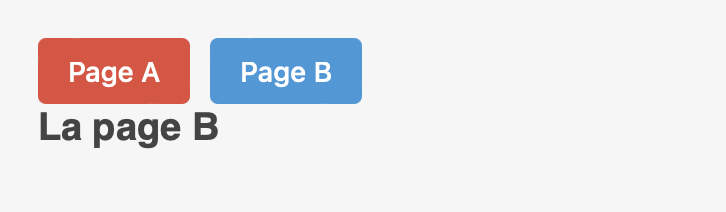
\includegraphics[width=7cm]{images/image29.png}
\end{center}
%%%%%%%%%%%%%%%%%%%%%%%%%%%%%%%%%%%%%%%%%%%%%%%%%%%

\section{Le composant KeepAlive}
\subsection{Le composant {\color{monOrange}KeepAlive}}
Le composant natif {\tt <KeepAlive>} permet de mettre en cache conditionnellement des composants lorsque l'on change dynamiquement de composant . En effet, par défaut une instance d'un composant {\color{monOrange}Vue} est démontée ( {\color{monOrange}unmounted}) lorsqu'il n'est plus affiché. Cela entraîne la perte de tout état du composant. Autrement dit, lorsqu'un composant n'est plus affiché, toutes les variables, notamment réactives, perdent leurs valeurs.

Lorsqu'un composant mis en cache avec {\tt <KeepAlive>} est retiré du {\color{monOrange}DOM}, il est mis dans l'état désactivé ({\tt deactivated}) au lieu d'être démonté ( {\tt unmounted}).

Lorsque le composant est remis sur le {\color{monOrange}DOM} aura alors l'état est activé ( {\tt activated}). Il suffit d'imbriquer, le ou les composants à l'intérieur du composant {\tt <KeepAlive>}, par exemple :
\begin{minted}[
mathescape,
framesep=2mm,
baselinestretch=1.2,
%fontsize=\footnotesize,
bgcolor=LightGray,
%linenos
]{html}
<KeepAlive>
  <Component :is="onglet" />
</KeepAlive>
\end{minted}

\subsection{Définir les composants à maintenir en vie avec {\color{monOrange}includes} et {\color{monOrange}exclude}}
Par défaut, {\tt <KeepAlive>} mis en cache tous les composants imbriqués. Il est possible de modifier ce comportement avec les {\color{monOrange}props include} et {\color{monOrange}exclude}. Pour utiliser cette fonctionnalité, il faut préalablement que les composants soient nommés en utilisant une deuxième balise {\color{monOrange}script} et en utilisant la propriété {\tt name}, comme ici :
\begin{minted}[
mathescape,
framesep=2mm,
baselinestretch=1.2,
%fontsize=\footnotesize,
bgcolor=LightGray,
%linenos
]{html}
<script lang="ts">
export default {
  name: 'PageB',
};
</script>
\end{minted}
Il suffit ensuite de préciser les composants à mettre en cache en utilisant {\color{monOrange}include} ou {\color{monOrange}exclude}:
\begin{minted}[
mathescape,
framesep=2mm,
baselinestretch=1.2,
%fontsize=\footnotesize,
bgcolor=LightGray,
%linenos
]{html}
<KeepAlive include="PageB">
  <Component :is="composants[selectedComponant]" />
</KeepAlive>
\end{minted}
Vous pouvez utiliser des {\color{monOrange}Regex}:
\begin{minted}[
mathescape,
framesep=2mm,
baselinestretch=1.2,
%fontsize=\footnotesize,
bgcolor=LightGray,
%linenos
]{html}
<KeepAlive include="/Page*/">
  <Component :is="composants[selectedComponant]" />
</KeepAlive>
\end{minted}
Passer plusieurs noms en utilisant des virgules :
\begin{minted}[
mathescape,
framesep=2mm,
baselinestretch=1.2,
%fontsize=\footnotesize,
bgcolor=LightGray,
%linenos
]{html}
<KeepAlive exclude="PageA, PageC">
  <Component :is="composants[selectedComponant]" />
</KeepAlive>
\end{minted}
Ou un tableau :
\begin{minted}[
mathescape,
framesep=2mm,
baselinestretch=1.2,
%fontsize=\footnotesize,
bgcolor=LightGray,
%linenos
]{html}
<KeepAlive exclude="['PageA', 'PageC']">
  <Component :is="composants[selectedComponant]" />
</KeepAlive>
\end{minted}
\subsection{Définir le maximum de composants mis en cache}
Si vous avez un très grand nombre de composants susceptibles d'être mis en cache, vous pouvez limiter le nombre maximal de composants à mettre en cache avec la {\color{monOrange}props max}. Il faut utiliser {\color{monOrange}v-bind} car nous passons un nombre (comme nous l'avions vu, sans {\color{monOrange}v-bind} les nombres sont passés comme des chaînes de caractères) :
\begin{minted}[
mathescape,
framesep=2mm,
baselinestretch=1.2,
%fontsize=\footnotesize,
bgcolor=LightGray,
%linenos
]{html}
<KeepAlive :max="10">
  <Component :is="activeComponent" />
</KeepAlive>
\end{minted}
\subsection{Les {\color{monOrange}hooks} utilisables}
Il est possible d'utiliser les {\tt hooks:} {\color{monOrange}activated()} et {\color{monOrange}deactivated()}.
\begin{minted}[
mathescape,
framesep=2mm,
baselinestretch=1.2,
%fontsize=\footnotesize,
bgcolor=LightGray,
%linenos
]{html}
<script setup lang="ts">
import { onActivated, onDeactivated } from 'vue'

onActivated(() => {
  // appelé à chaque activation du composant
})

onDeactivated(() => {
  // appelé à chaque désactivation du composant
})
</script>
\end{minted}

\subsection{Exemple}
On reprend l'exemple précédant et on modifie {\tt App.vue} de la façon suivante:
\begin{minted}[
mathescape,
framesep=2mm,
baselinestretch=1.2,
fontsize=\footnotesize,
bgcolor=LightGray,
%linenos
]{html}
<KeepAlive :max="5">
      <Component :is="composants[selectedComponant]" />
</KeepAlive>
\end{minted}
On modéfie {\tt PageA.vue} et {\tt PageB.vue}:
\begin{minted}[
mathescape,
framesep=2mm,
baselinestretch=1.2,
%fontsize=\footnotesize,
bgcolor=LightGray,
%linenos
]{html}
<template>
  <h3>La page A</h3>
  <br />
  <button class="btn mb-20" @click="count++">{{ count }}</button>
</template>

<script setup lang="ts">
import { ref, onDeactivated } from 'vue';

const count = ref(0);

onDeactivated(() => {
  count.value--;
});
</script>

<style scoped lang="scss"></style>
\end{minted}
puis on fait
\begin{minted}[
mathescape,
framesep=2mm,
baselinestretch=1.2,
fontsize=\footnotesize,
bgcolor=LightGray,
%linenos
]{html}
<template>
  <h3>La page B</h3>
  <br />
  <span>Utilisateur : {{ username }}</span>
  <input v-model="username" />
</template>

<script lang="ts">
export default {
  name: 'PageB',
};
</script>

<script setup lang="ts">
import { ref, onActivated } from 'vue';
const username = ref('');

onActivated(() => {
  username.value += '!';
});
</script>

<style scoped lang="scss"></style>
\end{minted}
On teste le resultat:
\begin{center}
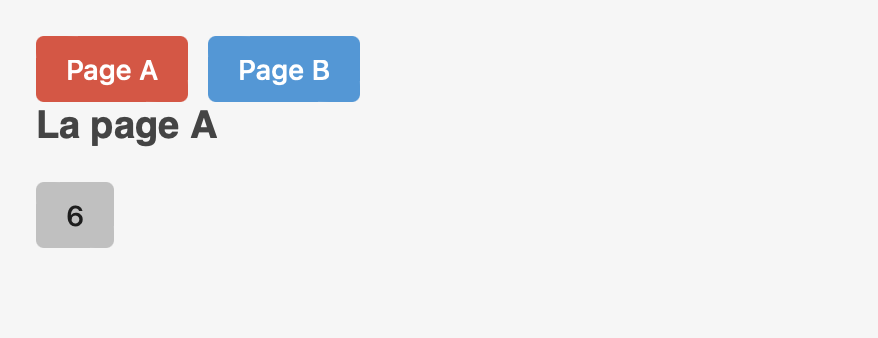
\includegraphics[width=7cm]{images/image30.png}
\end{center}


%%%%%%%%%%%%%%%%%%%%%%%%%%%%%%%%%%%%%%%%%%%%%%%%%%%%%%%%%%%%%

\section{Le composant Téléport}
\subsection{Le composant natif {\color{monOrange}Teleport}}
{\tt <Teleport>} est un composant natif permettant de {\em téléporter} une partie du {\color{monOrange}template} un composant sur un noeud du {\color{monOrange}DOM} qui existe en dehors de la branche du composant, ou même en dehors de l'application {\color{monOrange}Vue}.

Le scénario le plus commun est la modale : une partie d'un composant doit être affichée ailleurs sur le {\color{monOrange}DOM}, à l'extérieur de l'application. Nous voulons en effet que le bouton de la modale et la modale soient dans le même composant, car ils sont tous deux liés à l'état ouvert/fermé de la modale. Mais cela signifie que le modal sera rendu à côté du bouton, profondément imbriquée dans l'arbre des composants de l'application {\color{monOrange}Vue}. Cela peut créer des problèmes lors du positionnement de la modale avec du {\color{monOrange}CSS}. L'utilisation est très simple, il suffit d'imbriquer la partie du {\color{monOrange}template} "téléporter" dans des balises {\tt <Teleport>} et d'indiquer avec le {\color{monOrange}props to} sélecteur {\color{monOrange}CSS} ciblé :
\begin{minted}[
mathescape,
framesep=2mm,
baselinestretch=1.2,
%fontsize=\footnotesize,
bgcolor=LightGray,
%linenos
]{html}
<button @click="open = true">Ouvrir</button>

<Teleport to="body">
  <div v-if="open" class="modal">
    <p>Contenu de la modale</p>
    <button @click="open = false">Fermer</button>
  </div>
</Teleport>
\end{minted}
Il est possible de désactiver la téléportation du {\color{monOrange}template} en fonction de la valeur d'une variable en utilisant {\color{monOrange}disabled}:
\begin{minted}[
mathescape,
framesep=2mm,
baselinestretch=1.2,
fontsize=\footnotesize,
bgcolor=LightGray,
%linenos
]{html}
<Teleport :disabled="isMobile">
  ...
</Teleport>
\end{minted}
\subsection{Exemple}
\subsubsection*{App.vue}
\begin{minted}[
mathescape,
framesep=2mm,
baselinestretch=1.2,
%fontsize=\footnotesize,
bgcolor=LightGray,
%linenos
]{html}
<template>
  <Page />
</template>

<script setup lang="ts">
import Page from './Page.vue';
</script>

<style lang="scss">
@import './assets/scss/base.scss';
</style>
\end{minted}
\subsubsection*{Page.vue}
\begin{minted}[
mathescape,
framesep=2mm,
baselinestretch=1.2,
fontsize=\footnotesize,
bgcolor=LightGray,
%linenos
]{html}
<template>
  <div class="p-20 container">
    <h3>PAGE</h3>
    <Modal />
  </div>
</template>

<script setup lang="ts">
import Modal from './Modal.vue';
</script>

<style lang="scss">
.container {
  position: relative;
}
</style>
\end{minted}
\subsubsection*{Modal.vue}
\begin{minted}[
mathescape,
framesep=2mm,
baselinestretch=1.2,
fontsize=\footnotesize,
bgcolor=LightGray,
%linenos
]{html}
<template>
  <button @click="open = true" class="btn btn-primary">
    Confirmer l'achat
  </button>
  <Teleport to="body">
    <div
      v-if="open"
      @click="open = false"
      class="calc d-flex flex-row justify-content-center align-items-center"
    >
      <div @click.stop class="modal-container">
        <h3>Confirmation de votre commande</h3>
        <ul>
          <li>Du contenu</li>
          <li>Du contenu</li>
          <li>Du contenu</li>
        </ul>
        <button @click.stop="open = false" class="btn btn-danger">
          Confirmer la commande
        </button>
      </div>
    </div>
  </Teleport>
</template>

<script setup lang="ts">
import { ref } from 'vue';

const open = ref(false);
</script>

<style lang="scss">
.calc {
  position: absolute;
  top: 0;
  width: 100%;
  height: 100vh;
  background-color: rgba(0, 0, 0, 0.5);
  backdrop-filter: blur(2px);
}

.modal-container {
  background-color: white;
  border-radius: var(--border-radius);
  border: var(--border);
  padding: 30px;
}
</style>
\end{minted}
\begin{center}
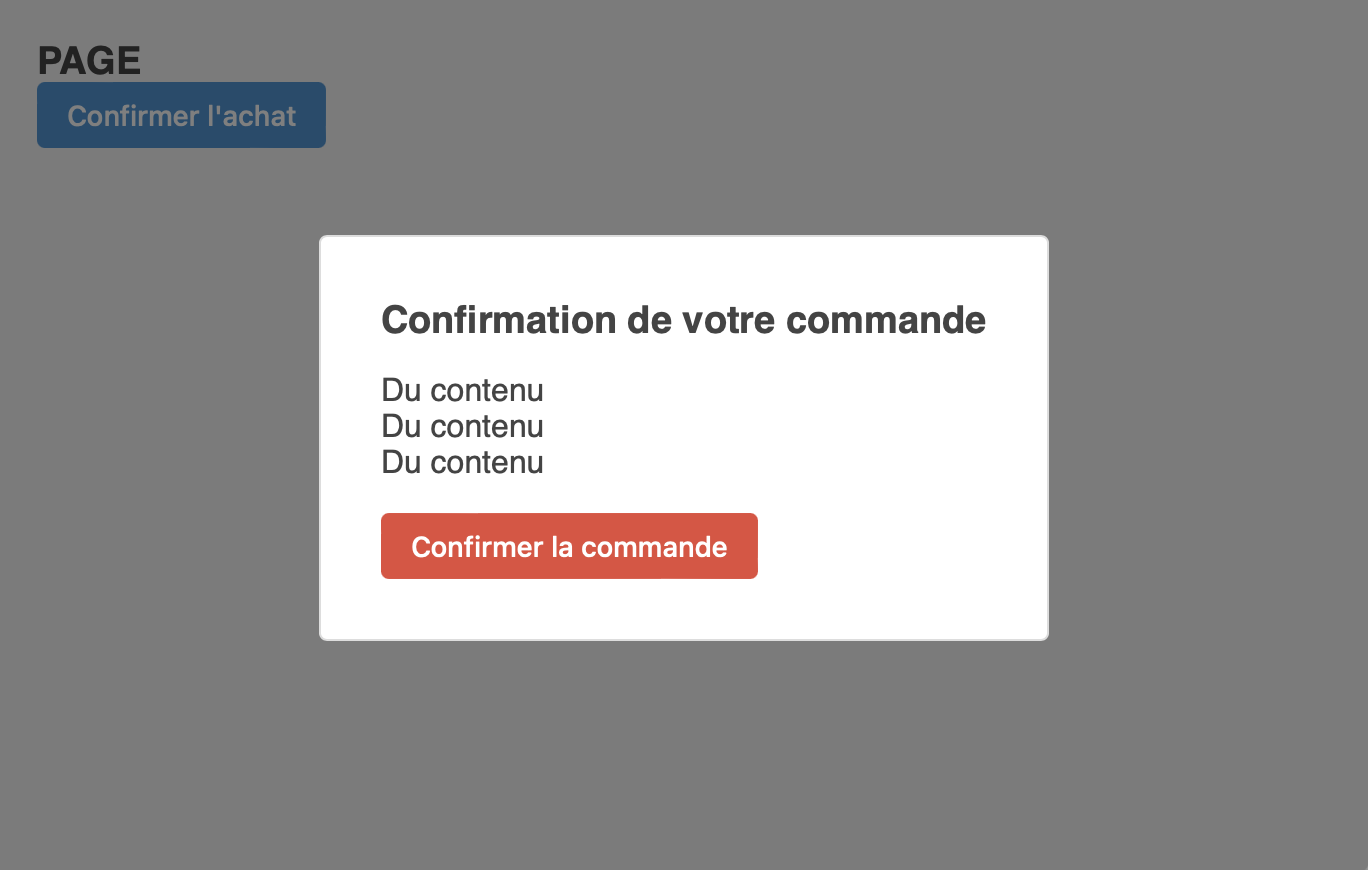
\includegraphics[width=10cm]{images/image31.png}
\end{center}
%%%%%%%%%%%%%%%%%%%%%%%%%%%%%%%%%%%%%%%%%%%%%%%%%%%%%%%%%%%%%%

\section{Le composant Suspense}
\subsection{Le composant {\tt <Suspense>}}
{\tt <Suspense>} est un composant natif permettant de gérer les dépendances asynchrones d'une branche de composants . Il permet d'afficher un {\color{monOrange}template} spécifique pendant le chargement des différentes ressources asynchrones. Les ressources asynchrones sont la plupart du temps des requêtes {\color{monOrange}HTTP} pour récupérer des données depuis une {\color{monOrange}API}. Il peut y avoir un composant qui a besoin d'une liste d'utilisateurs, un autre qui a besoin de favoris, un troisième de préférences utilisateur avec des requêtes différentes.

Sans {\color{monOrange}Suspense} il faut que chaque composant gère l'affichage d'un composant de chargement, des éventuelles erreurs etc. Cela permet de simplifier grandement la gestion des ressources asynchrones.

Le composant {\color{monOrange}Suspense} peut gérer deux types de dépendances asynchrones : les composants qui utilisent des {\color{monOrange}await} au premier niveau (c'est-à-dire pas imbriqué dans une fonction, directement dans les balises {\color{monOrange}script}) et les composants asynchrones .

Pour les composants avec {\color{monOrange}await} au premier niveau, le cas le plus courant est une requête {\color{monOrange}HTTP}:
\begin{minted}[
mathescape,
framesep=2mm,
baselinestretch=1.2,
%fontsize=\footnotesize,
bgcolor=LightGray,
%linenos
]{html}
<script setup>
const res = await fetch(...)
const posts = await res.json()
</script>
\end{minted}
\subsection{État de chargement}
Le composant {\color{monOrange}Suspense} à deux {\color{monOrange}slots} nommés : {\color{monOrange}\#default} et {\color{monOrange}\#fallback} . Chaque {\color{monOrange}slot} permet l'utilisation d'un unique enfant : que ce soit un composant ou un élément {\color{monOrange}HTML}:
\begin{minted}[
mathescape,
framesep=2mm,
baselinestretch=1.2,
%fontsize=\footnotesize,
bgcolor=LightGray,
%linenos
]{html}
<Suspense>
  <Dashboard />
  <template #fallback>
    Chargement...
  </template>
</Suspense>
\end{minted}
Lors du rendu initial, {\color{monOrange}Suspense} va afficher le {\color{monOrange}slot} par défaut (ici le composant {\color{monOrange}Dashbord}, car le {\color{monOrange}slot default} est l'élément qui n'a pas de nom). S'il rencontre une dépendance asynchrone, {\color{monOrange}Suspense} va entrer dans l'état en attente ( {\color{monOrange}pending state}). Pendant toute la durée de cet état, il affichera le {\color{monOrange}slot fallback}, ici {\tt <template \#fallback>}.

Lorsque tous les contenus asynchrones sont chargés ou qu'il n'y a aucune dépendance asynchrone, alors {\color{monOrange} Suspense} à l'état résolu ( {\color{monOrange}resolved state}) et le {\color{monOrange}slot} par défaut est affiché.

\subsection{Les événements émis}
Le composant {\color{monOrange}Suspense} émet trois événements :
\begin{itemize}
\item {\color{monOrange}pending:} émis lorsqu'il entre dans l'état pendinget donc qu'au moins une dépendance asynchrone a été détectée.
\item {\color{monOrange}resolve:} émis lorsqu'aucune dépendance asynchrone ne reste à charger.
\item {\color{monOrange}fallback:} émis lorsque le composant Suspense affiche le {\color{monOrange}slot fallbacklors} du chargement des dépendances asynchrones.

\end{itemize}
\subsection{Option {\color{monOrange}timeout}}
Lorsque le composant {\color{monOrange}Suspense} est dans l'état résolu, il ne retournera dans l'état en attente que si un composant dynamique est modifié et que la propriété {\color{monOrange}timeout} est définie. En effet, par défaut, {\color{monOrange}Suspense} affichera le composant par défaut et non le {\color{monOrange}fallback} pendant le chargement des dépendances asynchrones dans ce cas.

Il est possible de passer un nombre de millisecondes à {\color{monOrange}timeout} pour que {\color{monOrange}Suspense} affiche le {\color{monOrange}fallback} pendant le chargement, si les dépendances ne sont pas résolues pendant ce laps de temps.
\subsection{Exemple}
\subsubsection*{App.vue}
\begin{minted}[
mathescape,
framesep=2mm,
baselinestretch=1.2,
fontsize=\footnotesize,
bgcolor=LightGray,
%linenos
]{html}
<template>
  <h2>{{ evenement }}</h2>
  <Suspense
    @pending="myEvent('PENDING')"
    @fallback="myEvent('FALLBACK')"
    @resolve="myEvent('RESOLVE')"
  >
    <LazyList />
    <template #fallback>
      <h1>Chargement...</h1>
    </template>
  </Suspense>
</template>

<script setup lang="ts">
import { defineAsyncComponent, ref } from 'vue';

const evenement = ref('');
const LazyList = defineAsyncComponent(() => import('./Liste.vue'));

function myEvent(eventName: string) {
  console.log(eventName);
  evenement.value = eventName;
}
</script>

<style lang="scss"></style>
\end{minted}
\subsubsection*{Liste.vue}
\begin{minted}[
mathescape,
framesep=2mm,
baselinestretch=1.2,
fontsize=\footnotesize,
bgcolor=LightGray,
%linenos
]{html}
<template>
  <div class="p-20">
    <ul>
      <li v-for="user of state.users">{{ user.name }}</li>
    </ul>
  </div>
</template>

<script setup lang="ts">
import { reactive } from 'vue';

const state = reactive<{ users: any[] }>({ users: [] });

// Délai de 3secondes grâce à l'option delay de restapi
state.users = await (
  await fetch('https://restapi.fr/api/vueusers?delay=3')
).json();
</script>

<style lang="scss"></style>
\end{minted}
\begin{center}
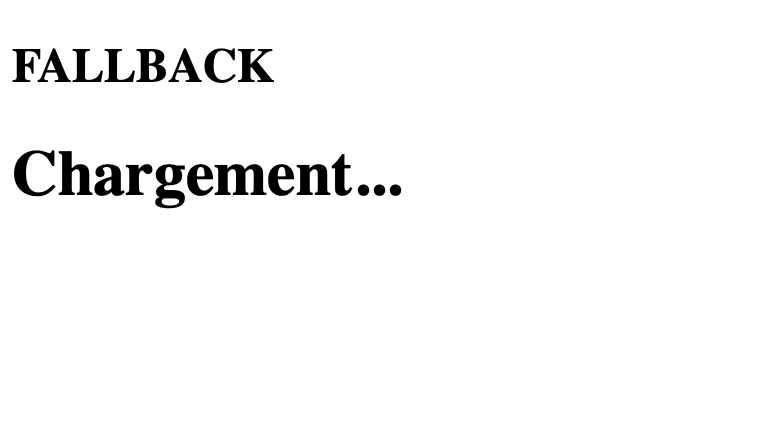
\includegraphics[width=7cm]{images/image32.png}
\end{center}

	\chapter{Projet Boutique - partie 3}
	\section{Introduction des fonctionnalités}
\subsection{Architecture des composants}
Voici l'arbre des composants que nous aurons à la fin du chapitre :
\begin{center}
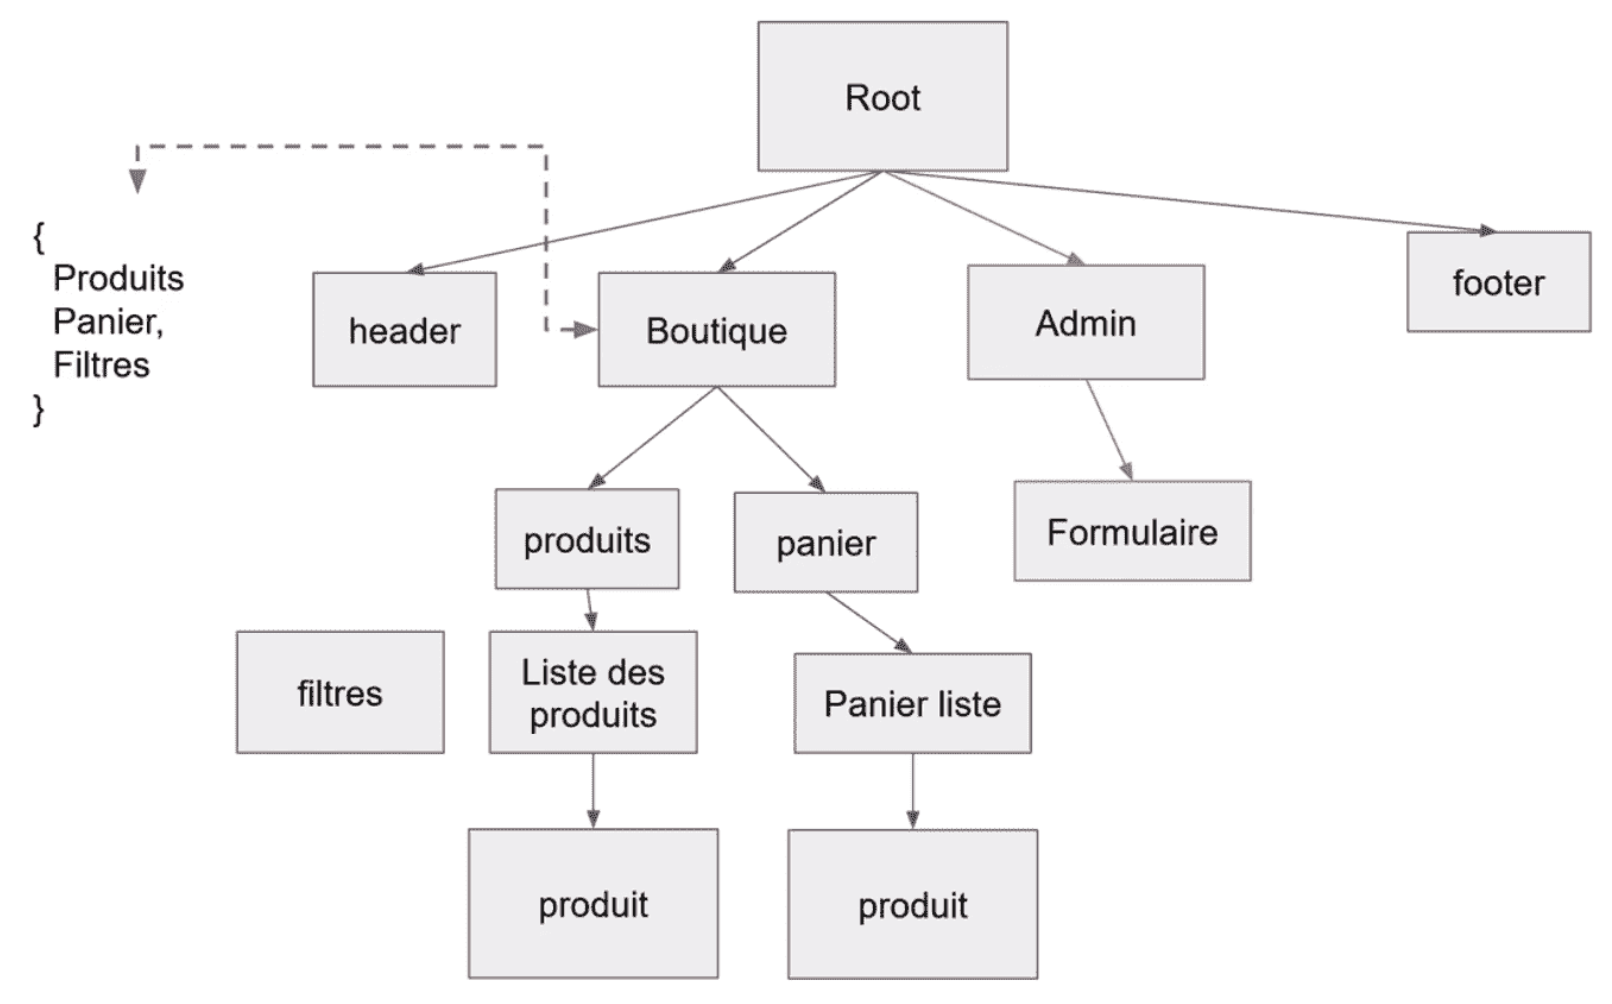
\includegraphics[width=10cm]{images/image33.png}
\end{center}

Notez que l'état des produits, du panier et des filtres sera contenu dans le composant Boutique.

\subsection{Création de nouveaux dossiers}
Dans le dossier srccréez un dossier features.

Dans ce dossier, créez les dossiers boutiqueet admin.

Dans le dossier boutiquecréez un dossier components. Déplacez-y les dossiers Cartet Shop.

Créez également dans boutiqueun dossier dataet un fichier Boutique.vue.

\subsection{Modification de App.vue}
La plupart de la logique dans le composant racine est déplacée dans le composant Boutique, nous n'avons donc plus que :
\begin{minted}[
mathescape,
framesep=2mm,
baselinestretch=1.2,
fontsize=\footnotesize,
bgcolor=LightGray,
%linenos
]{html}
<script setup lang="ts">
import TheHeader from './components/Header.vue';
import TheFooter from './components/Footer.vue';
import Boutique from './features/boutique/Boutique.vue';
</script>

<template>
  <div class="app-container">
    <TheHeader class="header" />
    <div class="app-content"><Component :is="Boutique" /></div>
    <TheFooter class="footer" />
  </div>
</template>

<style lang="scss">
@import './assets/scss/base.scss';
@import './assets/scss/debug.scss';

.app-container {
  min-height: 100vh;
  display: grid;
  grid-template-areas: 'header' 'app-content' 'footer';
  grid-template-rows: 48px auto 48px;
}

.header {  grid-area: header;}
.app-content {  grid-area: app-content;}
.footer {  grid-area: footer;}
</style>
\end{minted}

Notez bien l'utilisation du composant dynamique qui nous permettra de changer le composant affiché.

\subsection{Modification de Boutique.vue}
Voici le composant Boutiqueaprès y avoir déplacé toute la logique relative à la boutique :
\begin{minted}[
mathescape,
framesep=2mm,
baselinestretch=1.2,
fontsize=\footnotesize,
bgcolor=LightGray,
%linenos
]{html}
<script setup lang="ts">
import Shop from './components/Shop/Shop.vue';
import Cart from './components/Cart/Cart.vue';
import data from '../../data/product';
import { computed, reactive } from 'vue';
import type {
  FiltersInterface,
  ProductCartInterface,
  ProductInterface,
  FilterUpdate,
} from '../../interfaces';
import { DEFAULT_FILTERS } from '../../data/filters';

const state = reactive<{
  products: ProductInterface[];
  cart: ProductCartInterface[];
  filters: FiltersInterface;
}>({
  products: data,
  cart: [],
  filters: { ...DEFAULT_FILTERS },
});

function addProductToCart(productId: number): void {
  const product = state.products.find((product) => product.id === productId);
  if (product) {
    const productInCart = state.cart.find(
      (product) => product.id === productId
    );
    if (productInCart) {
      productInCart.quantity++;
    } else {
      state.cart.push({ ...product, quantity: 1 });
    }
  }
}

function removeProductFromCart(productId: number): void {
  const productFromCart = state.cart.find(
    (product) => product.id === productId
  );
  if (productFromCart?.quantity === 1) {
    state.cart = state.cart.filter((product) => product.id !== productId);
  } else {
    productFromCart.quantity--;
  }
}

function updateFilter(filterUpdate: FilterUpdate) {
  if (filterUpdate.search !== undefined) {
    state.filters.search = filterUpdate.search;
  } else if (filterUpdate.priceRange) {
    state.filters.priceRange = filterUpdate.priceRange;
  } else if (filterUpdate.category) {
    state.filters.category = filterUpdate.category;
  } else {
    state.filters = { ...DEFAULT_FILTERS };
  }
}

const cartEmpty = computed(() => state.cart.length === 0);

const filteredProducts = computed(() => {
  return state.products.filter((product) => {
    if (
      product.title
        .toLocaleLowerCase()
        .startsWith(state.filters.search.toLocaleLowerCase()) &&
      product.price >= state.filters.priceRange[0] &&
      product.price <= state.filters.priceRange[1] &&
      (product.category === state.filters.category ||
        state.filters.category === 'all')
    ) {
      return true;
    } else {
      return false;
    }
  });
});
</script>

<template>
  <div class="boutique-container" :class="{ 'grid-empty': cartEmpty }">
    <Shop
      @update-filter="updateFilter"
      :products="filteredProducts"
      :filters="state.filters"
      @add-product-to-cart="addProductToCart"
      class="shop"
    />
    <Cart
      v-if="!cartEmpty"
      :cart="state.cart"
      class="cart"
      @remove-product-from-cart="removeProductFromCart"
    />
  </div>
</template>

<style lang="scss">
.boutique-container {
  display: grid;
  grid-template-columns: 75% 25%;
}
.grid-empty {
  grid-template-columns: 100%;
}
.cart {
  background-color: white;
  border-left: var(--border);
}
</style>
\end{minted}

Code de la vidéo
Voici le code de la vidéo :
%%%%%%%%%%%%%%%%%%%%%%%%%%%%%%%%%%%%%%%%%%%%%%%%%%%%%%%%%%%%%%%%%%

\section{Navigation à l'aide d'un composant dynamique}
\subsection{Création du composant {\tt Admin}}
Dans le dossier {\tt src/features/admin} créer le composant {\color{monOrange}Admin.vue}:
\begin{minted}[
mathescape,
framesep=2mm,
baselinestretch=1.2,
fontsize=\footnotesize,
bgcolor=LightGray,
%linenos
]{html}
<script setup lang="ts"></script>

<template></template>

<style scoped lang="scss"></style>
\end{minted}
\subsection{Création du fichier {\tt type.ts}}
Dans le dossier {\color{monOrange}interfaces} créé le fichier {\tt type.ts} qui va contenir nos types littéraires :
\begin{minted}[
mathescape,
framesep=2mm,
baselinestretch=1.2,
fontsize=\footnotesize,
bgcolor=LightGray,
%linenos
]{html}
export type Page = 'Boutique' | 'Admin';
export type Category = 'gamer' | 'desktop' | 'streaming' | 'all';
\end{minted}
N'oubliez pas de modifier le fichier {\tt index.ts} dans le même dossier :
\begin{minted}[
mathescape,
framesep=2mm,
baselinestretch=1.2,
fontsize=\footnotesize,
bgcolor=LightGray,
%linenos
]{html}
export * from './Product.interface';
export * from './ProductCart.interface';
export * from './Filters.interface';
export * from './type';
\end{minted}
Ainsi que l'import dans {\tt Filters.interface.ts} et {\tt Product.interface.ts}:
\begin{minted}[
mathescape,
framesep=2mm,
baselinestretch=1.2,
fontsize=\footnotesize,
bgcolor=LightGray,
%linenos
]{html}
import type { Category } from './type';
\end{minted}
\subsection{Modification de {\tt App.vue}}
Dans le composant {\color{monOrange}App.vue} nous allons mettre en place les deux composants possibles dans le composant dynamique et la navigation entre les deux :
\begin{minted}[
mathescape,
framesep=2mm,
baselinestretch=1.2,
fontsize=\footnotesize,
bgcolor=LightGray,
%linenos
]{html}
<script setup lang="ts">
import TheHeader from './components/Header.vue';
import TheFooter from './components/Footer.vue';
import Boutique from './features/boutique/Boutique.vue';
import Admin from './features/admin/Admin.vue';
import { reactive, type Component as C } from 'vue';
import type { Page } from './interfaces';

const state = reactive<{
    page: Page
}>({
    page: 'Boutique'
})

const pages: { [s: string]: C } = {
    Boutique,
    Admin
}

function navigate(page: Page): void {
    state.page = page;
}
</script>

<template>
  <div class="app-container">
    <TheHeader @navigate="navigate" :page="state.page" class="header" />
    <div class="app-content">
      <Component :is="pages[state.page]" />
    </div>
    <TheFooter class="footer" />
  </div>
</template>

<style lang="scss">
@use './assets/scss/base.scss' as *;
@use './assets/scss/debug.scss' as *;

.app-container {
  min-height: 100vh;
  display: grid;
  grid-template-areas: 'header' 'app-content' 'footer';
  grid-template-rows: 48px auto 48px;
}

.header {
  grid-area: header;
}

.app-content {
  grid-area: app-content;
}

.footer {
  grid-area: footer;
}
</style>
\end{minted}
\subsection{Modification de {\tt Header.vue}}
Nous utilisons l'événement et la {\color{monOrange}props} définition dans le composant racine afin de pouvoir naviguer entre les composants {\color{monOrange}Admin} et {\color{monOrange}Boutique}:
\begin{minted}[
mathescape,
framesep=2mm,
baselinestretch=1.2,
fontsize=\footnotesize,
bgcolor=LightGray,
%linenos
]{html}
<script setup lang="ts">
import type { Page } from '@/interfaces';
defineProps<{
  page: Page;
}>();
const emit = defineEmits<{
  (e: 'navigate', page: Page): void;
}>();
</script>

<template>
  <header class="px-20 d-flex flex-row align-items-center">
    <a href="#" class="d-flex flex-row align-items-center mr-20">
      <img
        src="https://upload.wikimedia.org/wikipedia/commons/9/95/Vue.js_Logo_2.svg"
      />
      <span class="logo">Dyma</span>
    </a>
    <ul class="d-flex flex-row flex-fill">
      <li class="mr-10">
        <a
          :class="{ active: page === 'Boutique' }"
          @click="emit('navigate', 'Boutique')"
          >Boutique</a
        >
      </li>
      <li>
        <a
          :class="{ active: page === 'Admin' }"
          @click="emit('navigate', 'Admin')"
          >Admin</a
        >
      </li>
    </ul>
    <ul class="d-flex flex-row">
      <li class="mr-10">
        <a href="#">Inscription</a>
      </li>
      <li>
        <a href="#">Connexion</a>
      </li>
    </ul>
  </header>
</template>

<style lang="scss" scoped>
header {
  background-color: var(--primary-1);
  a {
    color: var(--text-primary-color);
    img {
      width: 20px;
      margin-right: 5px;
    }
    .logo {
      font-weight: 700;
      font-size: 20px;
    }
  }
  a.active {
    text-decoration: underline;
  }
}
</style>
\end{minted}
\subsection{Modification de {\tt src/assets/scss/base.scss}}
Ajoutez une classe pour nos cartes :
\begin{minted}[
mathescape,
framesep=2mm,
baselinestretch=1.2,
fontsize=\footnotesize,
bgcolor=LightGray,
%linenos
]{html}
.card {
    border: var(--border);
    border-radius: var(--border-radius);
    background-color:white;
    padding: 30px;
}
\end{minted}
\subsection{Création du composant {\tt ProductForm}}
Dans le dossier {\tt features/admin} créez un dossier {\color{monOrange}components} dans lequel vous mettez le fichier {\tt ProductForm.vue}:
\begin{minted}[
mathescape,
framesep=2mm,
baselinestretch=1.2,
fontsize=\footnotesize,
bgcolor=LightGray,
%linenos
]{html}
<script setup lang="ts"></script>

<template>
  <div class="card">
    <h1>Formulaire</h1>
  </div>
</template>

<style scoped lang="scss">
.card {
  width: 100%;
  max-width: 500px;
}
</style>
\end{minted}
\subsection{Modification du composant {\tt Admin}}
Nous utilisons ce composant dans le composant {\color{monOrange}Admin.vue}:
\begin{minted}[
mathescape,
framesep=2mm,
baselinestretch=1.2,
fontsize=\footnotesize,
bgcolor=LightGray,
%linenos
]{html}
<script setup lang="ts">
import ProductForm from './components/ProductForm.vue';
</script>

<template>
  <div
    class="
      admin-container
      d-flex
      flex-row
      justify-content-center
      align-items-center
    "
  >
    <ProductForm />
  </div>
</template>

<style scoped lang="scss">
.admin-container {
  height: 100%;
}
</style>
\end{minted}
%Code de la vidéo
%Voici le code de la vidéo :

\begin{center}
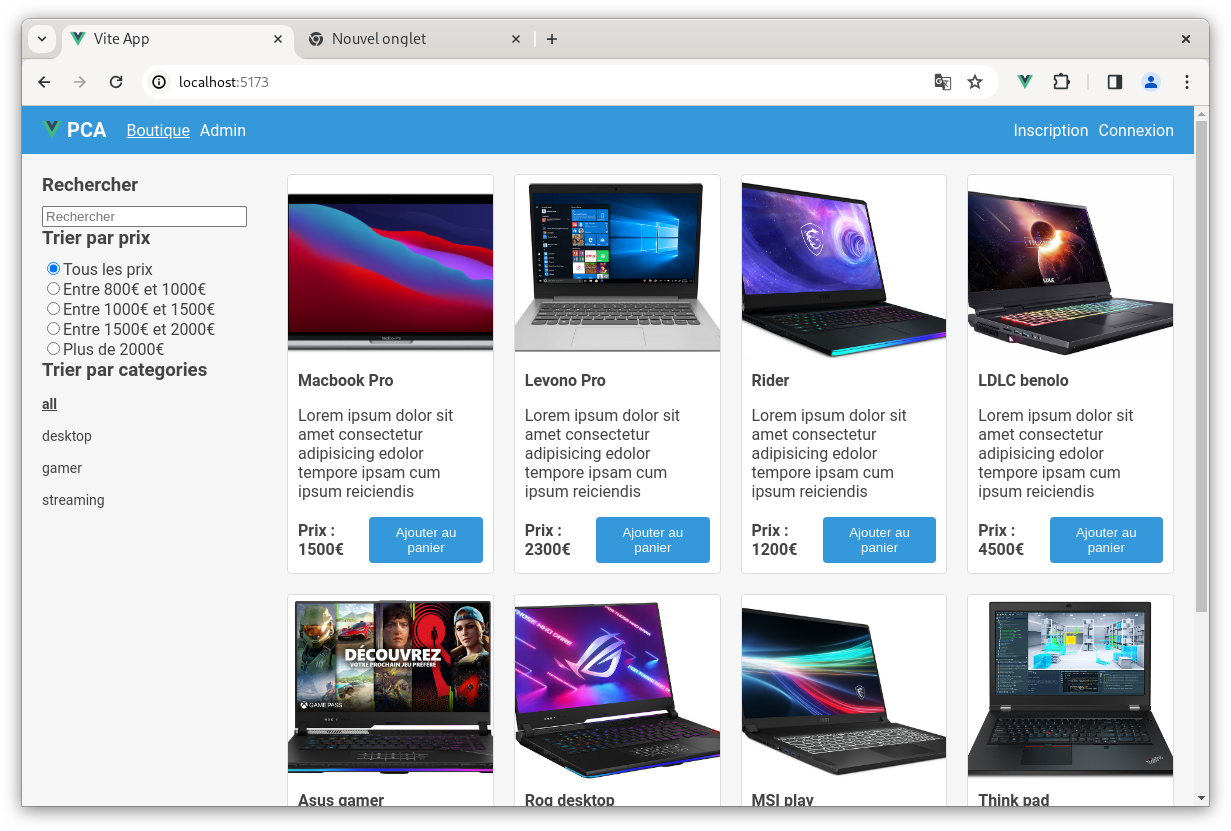
\includegraphics[width=12cm]{images/image34.png}
\end{center}

%%%%%%%%%%%%%%%%%%%%%%%%%%%%%%%%%%%%%%%%%%%%%%%%%%%%

\section{Mise en place du formulaire}
\subsection{Modification {\color{monOrange}debase.scss}}
Ajoutez les classes suivantes pour le formulaire :
\begin{minted}[
mathescape,
framesep=2mm,
baselinestretch=1.2,
fontsize=\footnotesize,
bgcolor=LightGray,
%linenos
]{html}
input, textarea, select {
    border: var(--border);
    border-radius: var(--border-radius);
    padding: 8px 15px;
}

label {
    font-size: 14px;
    font-weight: 500;
    color: var(--gray-3);
}

.form-error {
    color: var(--danger-1);
    font-size: 14px;
    font-weight: 500;
}
\end{minted}
\subsection{Modification de {\color{monOrange}ProductForm.vue}}
Nous mettons en place le formulaire et la validation :
\begin{minted}[
mathescape,
framesep=2mm,
baselinestretch=1.2,
fontsize=\footnotesize,
bgcolor=LightGray,
%linenos
]{html}
<script setup lang="ts">
import { useForm, useField } from 'vee-validate';
import { z } from 'zod';
import { toTypedSchema } from '@vee-validate/zod';

const required = { required_error: 'Veuillez renseigner ce champ' };
const validationSchema = toTypedSchema(
  z.object({
    title: z
      .string(required)
      .min(1, { message: 'Le titre doit faire au moins 1 caractère' })
      .max(20, { message: 'Le titre doit faire moins de 20 caractères' }),
    image: z.string(required),
    price: z
      .number(required)
      .min(0, { message: 'Le prix doit être supérieur à 0€' })
      .max(15000, { message: 'Le prix doit être inférieur à 150 00€' }),
    description: z
      .string(required)
      .min(10, { message: 'La description doit faire au moins 10 caractères' }),
    category: z.string(required),
  })
);

const { handleSubmit, isSubmitting } = useForm({
  validationSchema,
});

const title = useField('title');
const image = useField('image');
const price = useField('price');
const description = useField('description');
const category = useField('category');

const trySubmit = handleSubmit((formValues) => {
  console.log(formValues);
});
</script>

<template>
  <div class="card">
    <h3 class="mb-10">Ajouter un article</h3>
    <form @submit="trySubmit">
      <div class="d-flex flex-column mb-20">
        <label class="mb-5">*Titre</label>
        <input v-model="title.value.value" type="text" />
        <small class="form-error" v-if="title.errorMessage.value">{{
          title.errorMessage.value
        }}</small>
      </div>
      <div class="d-flex flex-column mb-20">
        <label class="mb-5">*Image</label>
        <input v-model="image.value.value" type="text" />
        <small class="form-error" v-if="image.errorMessage.value">{{
          image.errorMessage.value
        }}</small>
      </div>
      <div class="d-flex flex-column mb-20">
        <label class="mb-5">*Prix</label>
        <input v-model="price.value.value" type="number" />
        <small class="form-error" v-if="price.errorMessage.value">{{
          price.errorMessage.value
        }}</small>
      </div>
      <div class="d-flex flex-column mb-20">
        <label class="mb-5">*Description</label>
        <textarea v-model="(description.value.value as string)"></textarea>
        <small class="form-error" v-if="description.errorMessage.value">{{
          description.errorMessage.value
        }}</small>
      </div>
      <div class="d-flex flex-column mb-20">
        <label class="mb-5">*Catégorie</label>
        <select v-model="category.value.value">
          <option value disabled>Choisissez une catégorie</option>
          <option value="gamer">Jeu</option>
          <option value="desktop">Bureautique</option>
          <option value="streaming">Stream</option>
        </select>
        <small class="form-error" v-if="category.errorMessage.value">{{
          category.errorMessage.value
        }}</small>
      </div>
      <button class="btn btn-primary" :disabled="isSubmitting">
        Sauvegarder
      </button>
    </form>
  </div>
</template>

<style scoped lang="scss">
.card {
  width: 100%;
  max-width: 500px;
}
</style>
\end{minted}
{\tt image.value.value:} permet d'accéder à la propriété {\color{monOrange}value} retournée par {\color{monOrange}useField}, comme elle contient une {\color{monOrange}ref} qui est imbriquée dans l'objet, il n'y a pas d'accès automatique par {\color{monOrange}Vue} à la propriété {\color{monOrange}value} de la {\color{monOrange}ref} côté {\color{monOrange}template}( {\color{monOrange}unpacking}). Il faut donc y nous-mêmes.


%Code de la vidéo
%Voici le code de la vidéo :

\begin{center}
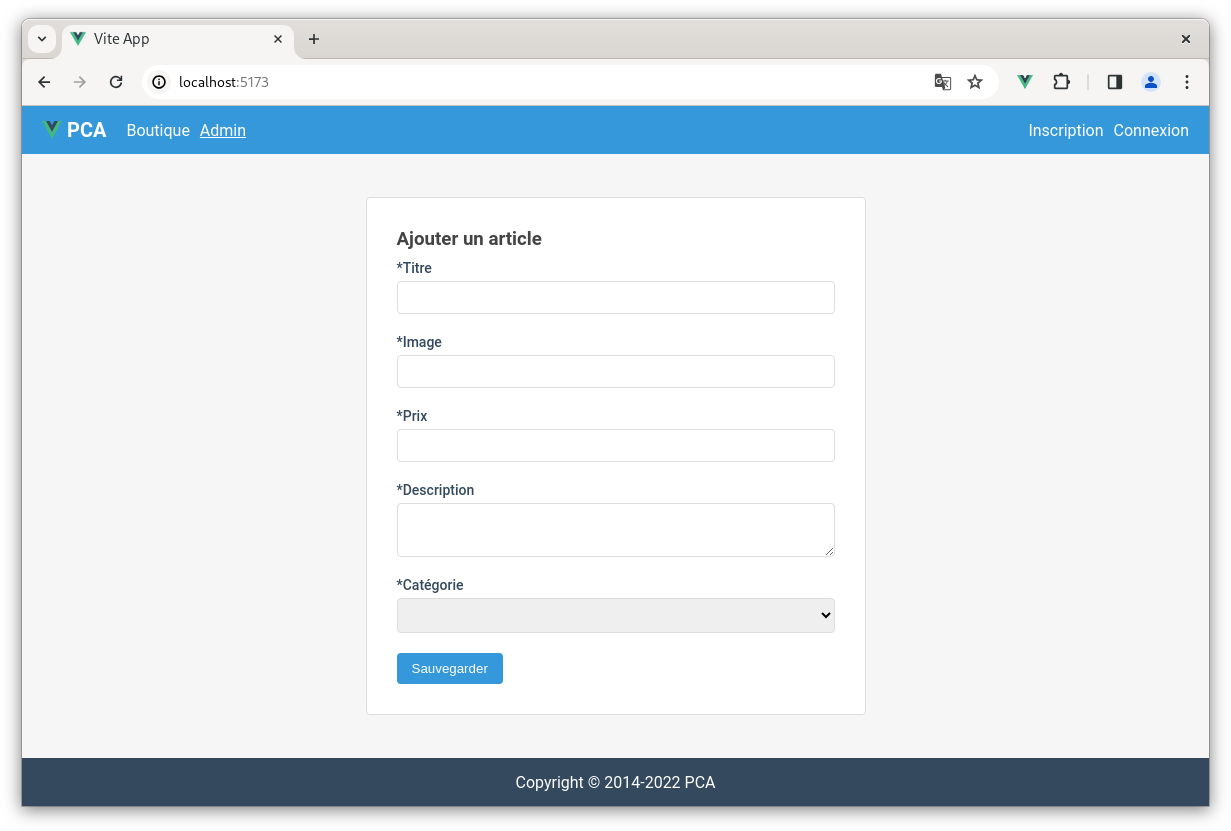
\includegraphics[width=12cm]{images/image35.png}
\end{center}

%%%%%%%%%%%%%%%%%%%%%%%%%%%%%%%%%%%%%%%%%%%%%%%%%%%%%%%

\section{Envoi du formulaire}
\subsection{Modification de {\color{monOrange}ProductForm.vue}}
Nous mettons en place l'envoi du formulaire au serveur {\color{monOrange}REST API}:
\begin{minted}[
mathescape,
framesep=2mm,
baselinestretch=1.2,
fontsize=\footnotesize,
bgcolor=LightGray,
%linenos
]{html}
<script setup lang="ts">
import { useForm, useField } from 'vee-validate';
import { z } from 'zod';
import { toTypedSchema } from '@vee-validate/zod';
import { onMounted, ref } from 'vue';

const firstInput = ref<HTMLInputElement | null>(null);
onMounted(() => {
  firstInput.value?.focus();
});

const required = { required_error: 'Veuillez renseigner ce champ' };
const validationSchema = toTypedSchema(
  z.object({
    title: z
      .string(required)
      .min(1, { message: 'Le titre doit faire au moins 1 caractère' })
      .max(20, { message: 'Le titre doit faire moins de 20 caractères' }),
    image: z.string(required),
    price: z
      .number(required)
      .min(0, { message: 'Le prix doit être supérieur à 0€' })
      .max(15000, { message: 'Le prix doit être inférieur à 150 00€' }),
    description: z
      .string(required)
      .min(10, { message: 'La description doit faire au moins 10 caractères' }),
    category: z.string(required),
  })
);

const { handleSubmit, isSubmitting } = useForm({
  validationSchema,
});

const title = useField('title');
const image = useField('image');
const price = useField('price');
const description = useField('description');
const category = useField('category');

const trySubmit = handleSubmit(async (formValues, { resetForm }) => {
  try {
    await fetch('https://restapi.fr/api/projetproducts', {
      method: 'POST',
      body: JSON.stringify(formValues),
      headers: {
        'Content-Type': 'application/json',
      },
    });
    resetForm();
    firstInput.value?.focus();
  } catch (e) {
    console.log(e);
  }
});
</script>

<template>
  <div class="card">
    <h3 class="mb-10">Ajouter un article</h3>
    <form @submit="trySubmit">
      <div class="d-flex flex-column mb-20">
        <label class="mb-5">*Titre</label>
        <input ref="firstInput" v-model="title.value.value" type="text" />
        <small class="form-error" v-if="title.errorMessage.value">{{
          title.errorMessage.value
        }}</small>
      </div>
      <div class="d-flex flex-column mb-20">
        <label class="mb-5">*Image</label>
        <input v-model="image.value.value" type="text" />
        <small class="form-error" v-if="image.errorMessage.value">{{
          image.errorMessage.value
        }}</small>
      </div>
      <div class="d-flex flex-column mb-20">
        <label class="mb-5">*Prix</label>
        <input v-model="price.value.value" type="number" />
        <small class="form-error" v-if="price.errorMessage.value">{{
          price.errorMessage.value
        }}</small>
      </div>
      <div class="d-flex flex-column mb-20">
        <label class="mb-5">*Description</label>
        <textarea v-model="(description.value.value as string)"></textarea>
        <small class="form-error" v-if="description.errorMessage.value">{{
          description.errorMessage.value
        }}</small>
      </div>
      <div class="d-flex flex-column mb-20">
        <label class="mb-5">*Catégorie</label>
        <select v-model="category.value.value">
          <option value disabled>Choisissez une catégorie</option>
          <option value="gamer">Jeu</option>
          <option value="desktop">Bureautique</option>
          <option value="streaming">Stream</option>
        </select>
        <small class="form-error" v-if="category.errorMessage.value">{{
          category.errorMessage.value
        }}</small>
      </div>
      <button class="btn btn-primary" :disabled="isSubmitting">
        Sauvegarder
      </button>
    </form>
  </div>
</template>

<style scoped lang="scss">
.card {
  width: 100%;
  max-width: 500px;
}
</style>
\end{minted}
\subsection{Modification de {\color{monOrange}Product.interface.ts}}
Nous modifions la propriété {\color{monOrange}id} car {\color{monOrange}MongoDB} (base de données utilisées pour la sauvegarde) utilisons la propriété {\color{monOrange}\_id} et nous ajoutons la propriété {\color{monOrange}createdAt} qui contient la date de création au format {\color{monOrange}ISO 8601}:
\begin{minted}[
mathescape,
framesep=2mm,
baselinestretch=1.2,
fontsize=\footnotesize,
bgcolor=LightGray,
%linenos
]{javascript}
import type { Category } from './type';

export interface ProductInterface {
  _id: string;
  createdAt: string;
  title: string;
  image: string;
  price: number;
  description: string;
  category: Category;
}
\end{minted}
\subsection{Création de {\tt src/data/seed.ts}}
Nous créons une fonction pour ajouter des données dans le service {\color{monOrange}restapi.fr} s'il n'y en a pas :
\begin{minted}[
mathescape,
framesep=2mm,
baselinestretch=1.2,
fontsize=\footnotesize,
bgcolor=LightGray,
%linenos
]{javascript}
import data from './product';

export async function seed(collectionName: string) {
  await fetch(`https://restapi.fr/api/${collectionName}`, {
    method: 'POST',
    body: JSON.stringify(data),
    headers: {
      'Content-Type': 'application/json',
    },
  });
}
\end{minted}
%$
\subsection{Modification de {\color{monOrange}App.vue}}
Nous appelons notre fonction permettant d'enregistrer nos données initiales, n'oubliez pas de la commenter après l'avoir exécuté une fois :
\begin{minted}[
mathescape,
framesep=2mm,
baselinestretch=1.2,
fontsize=\footnotesize,
bgcolor=LightGray,
%linenos
]{html}
<script setup lang="ts">
import TheHeader from './components/Header.vue';
import TheFooter from './components/Footer.vue';
import Boutique from './features/boutique/Boutique.vue';
import Admin from './features/admin/Admin.vue';
import { reactive, type Component as C } from 'vue';
import type { Page } from './interfaces';
import { seed } from './data/seed';

const state = reactive<{
    page: Page
}>({
    page: 'Boutique'
})

const pages: { [s: string]: C } = {
    Boutique,
    Admin
}

function navigate(page: Page): void {
    state.page = page;
}

// seed('projetproducts'); N’oubliez pas de commenter !
</script>

<template>
  <div class="app-container">
    <TheHeader @navigate="navigate" :page="state.page" class="header" />
    <div class="app-content">
      <Component :is="pages[state.page]" />
    </div>
    <TheFooter class="footer" />
  </div>
</template>

<style lang="scss">
@use './assets/scss/base.scss' as *;
@use './assets/scss/debug.scss' as *;

.app-container {
  min-height: 100vh;
  display: grid;
  grid-template-areas: 'header' 'app-content' 'footer';
  grid-template-rows: 48px auto 48px;
}

.header {
  grid-area: header;
}

.app-content {
  grid-area: app-content;
}

.footer {
  grid-area: footer;
}
</style>
\end{minted}

\begin{center}
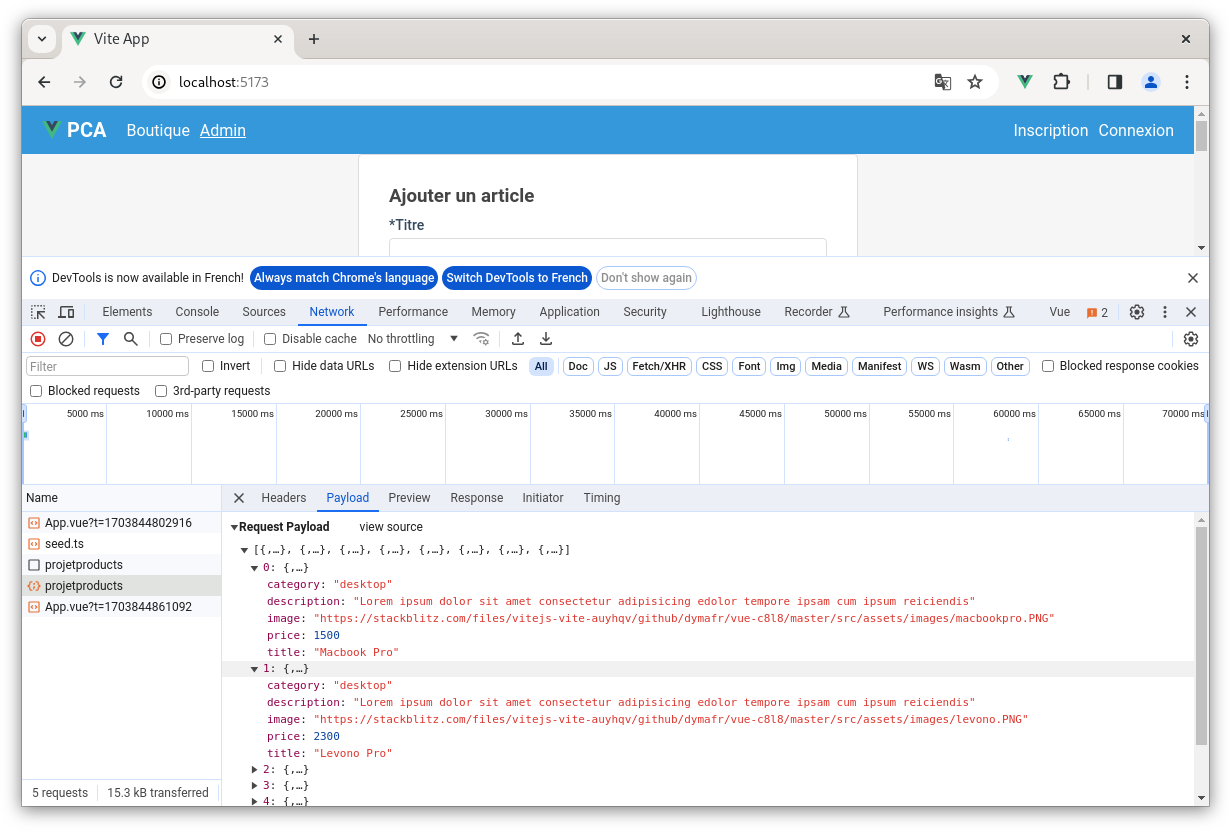
\includegraphics[width=12cm]{images/image36.png}
\end{center}

%%%%%%%%%%%%%%%%%%%%%%%%%%%%%%%%%%%%%%%%%%%%%%%%%%

\section{Récupération des produits}
\subsection{Modification de {\color{monOrange}Boutique.vue}}
Nous modifions le composant {\color{monOrange}Boutique} pour récupérer les produits :
\begin{minted}[
mathescape,
framesep=2mm,
baselinestretch=1.2,
fontsize=\footnotesize,
bgcolor=LightGray,
%linenos
]{html}
<script setup lang="ts">
import Shop from './components/Shop/Shop.vue';
import Cart from './components/Cart/Cart.vue';
import { computed, reactive } from 'vue';
import type {
  FiltersInterface,
  ProductCartInterface,
  ProductInterface,
  FilterUpdate,
} from '../../interfaces';
import { DEFAULT_FILTERS } from './data/filters';

const state = reactive<{
  products: ProductInterface[];
  cart: ProductCartInterface[];
  filters: FiltersInterface;
}>({
  products: [],
  cart: [],
  filters: { ...DEFAULT_FILTERS },
});

const products = await (
  await fetch('https://restapi.fr/api/projetproducts')
).json();
if (Array.isArray(products)) {
  state.products = products;
} else {
  state.products = [products];
}

function addProductToCart(productId: string): void {
  const product = state.products.find((product) => product._id === productId);
  if (product) {
    const productInCart = state.cart.find(
      (product) => product._id === productId
    );
    if (productInCart) {
      productInCart.quantity++;
    } else {
      state.cart.push({ ...product, quantity: 1 });
    }
  }
}

function removeProductFromCart(productId: string): void {
  const productFromCart = state.cart.find(
    (product) => product._id === productId
  );
  if (productFromCart?.quantity === 1) {
    state.cart = state.cart.filter((product) => product._id !== productId);
  } else {
    productFromCart.quantity--;
  }
}

function updateFilter(filterUpdate: FilterUpdate) {
  if (filterUpdate.search !== undefined) {
    state.filters.search = filterUpdate.search;
  } else if (filterUpdate.priceRange) {
    state.filters.priceRange = filterUpdate.priceRange;
  } else if (filterUpdate.category) {
    state.filters.category = filterUpdate.category;
  } else {
    state.filters = { ...DEFAULT_FILTERS };
  }
}

const cartEmpty = computed(() => state.cart.length === 0);

const filteredProducts = computed(() => {
  return state.products.filter((product) => {
    if (
      product.title
        .toLocaleLowerCase()
        .startsWith(state.filters.search.toLocaleLowerCase()) &&
      product.price >= state.filters.priceRange[0] &&
      product.price <= state.filters.priceRange[1] &&
      (product.category === state.filters.category ||
        state.filters.category === 'all')
    ) {
      return true;
    } else {
      return false;
    }
  });
});
</script>

<template>
  <div class="boutique-container" :class="{ 'grid-empty': cartEmpty }">
    <Shop
      @update-filter="updateFilter"
      :products="filteredProducts"
      :filters="state.filters"
      @add-product-to-cart="addProductToCart"
      class="shop"
    />
    <Cart
      v-if="!cartEmpty"
      :cart="state.cart"
      class="cart"
      @remove-product-from-cart="removeProductFromCart"
    />
  </div>
</template>

<style scoped lang="scss">
.boutique-container {
  display: grid;
  grid-template-columns: 75% 25%;
}
.grid-empty {
  grid-template-columns: 100%;
}
.cart {
  background-color: white;
  border-left: var(--border);
}
</style>
\end{minted}
Nous avons un {\color{monOrange}await} au premier niveau dans les balises {\color{monOrange}script} ce qui permet d'enregistrer ce composant comme ayant une dépendance asynchrone avec {\color{monOrange}Suspense}. N'oubliez pas de modifier l'utilisation des propriétés {\color{monOrange}id} par la propriété {\color{monOrange}\_id}.

\subsection{Modification de {\color{monOrange}App.vue}}
Nous utilisons Suspensepour attendre le chargement des produits :
\begin{minted}[
mathescape,
framesep=2mm,
baselinestretch=1.2,
fontsize=\footnotesize,
bgcolor=LightGray,
%linenos
]{html}
<template>
  <div class="app-container">
    <TheHeader @navigate="navigate" :page="state.page" class="header" />
    <div class="app-content">
      <Suspense>
        <Component :is="pages[state.page]" />
      </Suspense>
    </div>
    <TheFooter class="footer" />
  </div>
</template>
\end{minted}
\subsection{Modification du type de {\tt productId} et de la propriété {\tt id}}
Il faut modifier le type de {\color{monOrange}productId} en {\color{monOrange}string} et la propriété {\color{monOrange}id} des {\color{monOrange}products} par {\color{monOrange}\_id} dans les composants : {\color{monOrange}Shop.vue, ShopProductList.vue, ShopProduct.vue, Cart.vue, CartProductList.vue} et {\color{monOrange}CartProduct.vue}.

\begin{center}
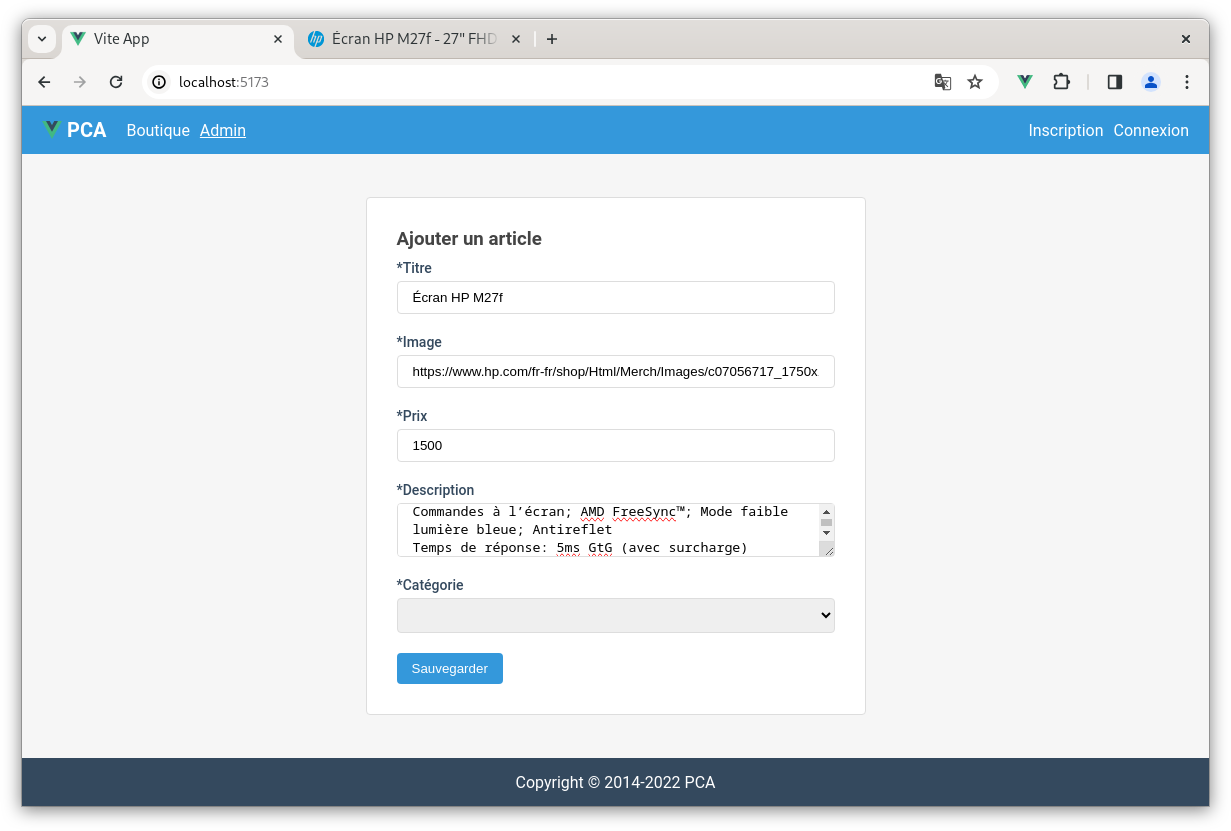
\includegraphics[width=10cm]{images/image37.png}
\end{center}

%%%%%%%%%%%%%%%%%%%%%%%%%%%%%%%%%%%%%%%%%%%%%%%%%%%%%%%%%%%%

\section{Amélioration du CSS}
\subsection{Modification de {\color{monOrange}App.vue}}
Modifiez le style du composant {\color{monOrange}App}:
\begin{minted}[
mathescape,
framesep=2mm,
baselinestretch=1.2,
fontsize=\footnotesize,
bgcolor=LightGray,
%linenos
]{html}
<style lang="scss">
@use './assets/scss/base.scss' as *;
@use './assets/scss/debug.scss' as *;

.app-container {
  height: 100vh;
  display: grid;
  grid-template-areas: 'header' 'app-content' 'footer';
  grid-template-rows: 48px auto 48px;
}

.header {
  grid-area: header;
}

.app-content {
  grid-area: app-content;
}

.footer {
  grid-area: footer;
}
</style>
\end{minted}
\subsection{Modification de {\color{monOrange}Shop.vue}}
Nous modifions le composant {\color{monOrange}Shop.vue} pour rendre {\color{monOrange}scrollable} la liste des produits :
\begin{minted}[
mathescape,
framesep=2mm,
baselinestretch=1.2,
fontsize=\footnotesize,
bgcolor=LightGray,
%linenos
]{html}
<script setup lang="ts">
import type {
  FiltersInterface,
  ProductInterface,
  FilterUpdate,
} from '../../interfaces';
import ShopProductList from './ShopProductList.vue';
import ShopFilters from './ShopFilters.vue';

defineProps<{
  products: ProductInterface[];
  filters: FiltersInterface;
}>();

const emit = defineEmits<{
  (e: 'addProductToCart', productId: string): void;
  (e: 'updateFilter', updateFilter: FilterUpdate): void;
}>();
</script>

<template>
  <div class="d-flex flex-row">
    <ShopFilters
      :filters="filters"
      :nbr-of-products="products.length"
      @update-filter="emit('updateFilter', $event)"
      class="shop-filter"
    />
    <ShopProductList
      class="flex-fill scrollable"
      @add-product-to-cart="emit('addProductToCart', $event)"
      :products="products"
    />
  </div>
</template>

<style lang="scss" scoped>
.scrollable {
  overflow-y: auto;
  height: calc(100vh - 96px);
}

.shop-filter {
  flex: 0 0 200px;
}
</style>
\end{minted}
\subsection{Création du fichier {\tt \_mixins.scss}}
Dans le dossier {\tt src/assets/scss} créez le fichier {\color{monOrange}\_mixins.scss}:
\begin{minted}[
mathescape,
framesep=2mm,
baselinestretch=1.2,
fontsize=\footnotesize,
bgcolor=LightGray,
%linenos
]{html}
@mixin sm {
  @media (min-width: 576px) {
    @content;
  }
}

@mixin md {
  @media (min-width: 768px) {
    @content;
  }
}

@mixin lg {
  @media (min-width: 992px) {
    @content;
  }
}

@mixin xl {
  @media (min-width: 1200px) {
    @content;
  }
}
\end{minted}
\subsection{Modification de {\color{monOrange}ShopProductList.vue}}
Nous utilisons nos {\color{monOrange}mixins} pour rendre la liste des produits {\color{monOrange}responsive} (c'est-à-dire qui s'adapte à la taille de l'écran) :
\begin{minted}[
mathescape,
framesep=2mm,
baselinestretch=1.2,
fontsize=\footnotesize,
bgcolor=LightGray,
%linenos
]{html}
<script setup lang="ts">
import type { ProductInterface } from '@/interfaces';
import ShopProduct from './ShopProduct.vue';

defineProps<{
  products: ProductInterface[];
}>();

const emit = defineEmits<{
  (e: 'addProductToCart', productId: string): void;
}>();
</script>

<template>
  <div class="grid p-20">
    <ShopProduct
      @add-product-to-cart="emit('addProductToCart', $event)"
      v-for="product of products"
      :product="product"
      :key="product._id"
    />
  </div>
</template>

<style lang="scss" scoped>
@use '../../../../assets/scss/mixins' as m;
.grid {
  display: grid;
  grid-template-columns: 1fr;
  @include m.md {
    grid-template-columns: 1fr 1fr;
  }
  @include m.lg {
    grid-template-columns: 1fr 1fr 1fr;
  }
  @include m.xl {
    grid-template-columns: 1fr 1fr 1fr 1fr;
  }
  grid-auto-rows: 400px;
  gap: 20px;
}
</style>
\end{minted}

%$
{\em Si vous ne comprenez pas le code revoyez les chapitres sur {\color{monOrange}Sass} et les {\color{monOrange}mixins} dans le cours {\color{monOrange}HTML \& CSS} .

\begin{center}
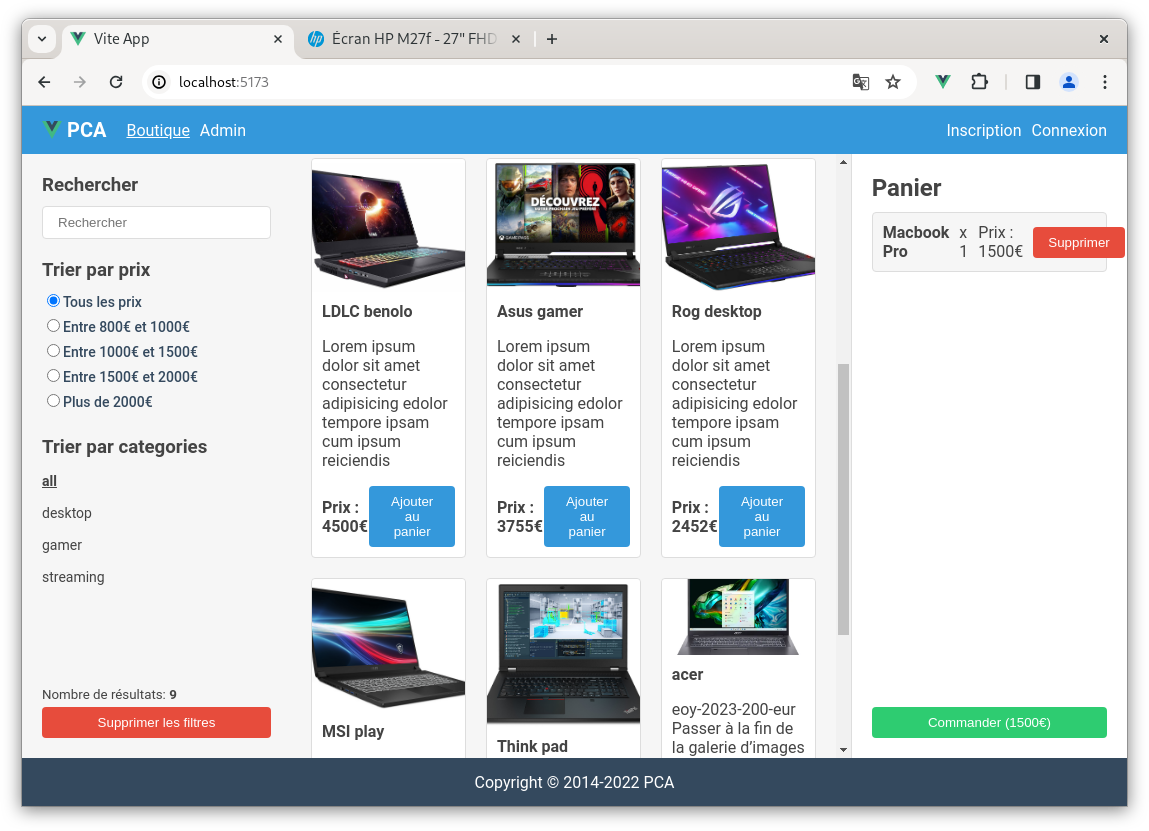
\includegraphics[width=10cm]{images/image38.png}
\end{center}

    \tableofcontents    

% Fin du document
\end{document}
